\documentclass[a4paper]{book}
\usepackage[
	%urlbordercolor = {1 1 1},
	%linkbordercolor = {1 1 1},
	%citebordercolor = {1 1 1},
	urlcolor = blue,
	colorlinks = true,
	citecolor = black,
	linkcolor = black]{hyperref}
\usepackage{graphicx}
\usepackage{xltxtra}
\usepackage{fancyhdr}
\usepackage{booktabs}
\usepackage{indentfirst}
\usepackage{framed,color}
\usepackage{caption}
\usepackage{longtable}
\captionsetup{font=bf,position=below}

\usepackage{ctable}

\definecolor{shadecolor}{gray}{0.90}

\setromanfont[Mapping=tex-text,BoldFont={* Bold}]{Helvetica}
\setmonofont[Scale=.85]{Andale Mono}

\XeTeXlinebreaklocale{en}


\settowidth{\parindent}{\qquad}

\title{Ruby on Rails 4.1}
\author{Stefan Wintermeyer}

\makeatletter
\let\savedauthor=\@author
\let\savedtitle=\@title
\def\imgwidth{.6\linewidth}
\def\maxwidth{\ifdim\Gin@nat@width>\imgwidth\imgwidth
\else\Gin@nat@width\fi}
\makeatother

\title{\textbf{\savedtitle}}
\author{\textbf{\savedauthor}\thanks{}}
\def\w3cdtfymd{\the\year-\ifnum\month<10 0\fi\the\month-\ifnum\day<10 0\fi\the\day}
\date{\w3cdtfymd}
\renewcommand{\thefootnote}{\fnsymbol{footnote}}

\makeatletter
  \setlength\headheight{12\p@}
  \setlength\headsep   {.25in}
  \setlength\topskip   {10\p@}
  \setlength\footskip{.35in}
  \setlength\textwidth{400\p@}
  
  \setlength\@tempdima{\paperheight}
  \addtolength\@tempdima{-2in}
  \divide\@tempdima\baselineskip
  \@tempcnta=\@tempdima
  \setlength\textheight{\@tempcnta\baselineskip}
  \addtolength\textheight{\topskip}
  
  \setlength\@tempdima        {\paperwidth}
  \addtolength\@tempdima      {-\textwidth}
  \setlength\oddsidemargin    {\paperwidth}
  \addtolength\oddsidemargin  {-2.35in}
  \addtolength\oddsidemargin  {-\textwidth}
  \setlength\marginparwidth   {0pt}
  \@settopoint\oddsidemargin
  \@settopoint\marginparwidth
  \setlength\evensidemargin  {\paperwidth}
  \addtolength\evensidemargin{-2.35in}
  \addtolength\evensidemargin{-\textwidth}
  \@settopoint\evensidemargin
  
  \setlength\topmargin{\paperheight}
  \addtolength\topmargin{-2in}
  \addtolength\topmargin{-\headheight}
  \addtolength\topmargin{-\headsep}
  \addtolength\topmargin{-\textheight}
  \addtolength\topmargin{-\footskip}     % this might be wrong!
  \addtolength\topmargin{-.5\topmargin}
  \@settopoint\topmargin
\makeatother

\fancypagestyle{plain}{\fancyhf{}\fancyfoot[LE,RO]{\footnotesize\textbf\thepage}}
\pagestyle{plain}

\renewcommand{\headrulewidth}{0pt}
\renewcommand{\footrulewidth}{0pt}

\newcounter{img}[chapter]
\renewcommand{\theimg}{\thechapter.\arabic{img}}
\newcommand{\img}[1]{\begin{figure}[ht!]
	\refstepcounter{img}
	\label{img:\theimg}
	\centering\IfFileExists{figures/\theimg.pdf}{\includegraphics[width=\maxwidth]{figures/\theimg.pdf}}{\includegraphics[width=\maxwidth]{figures/\theimg.png}}

	\caption{#1}
\end{figure}}

\newcounter{tab}[chapter]
\renewcommand{\thetab}{\thechapter.\arabic{tab}}

\newcommand{\prechap}{Chapter }
\newcommand{\postchap}{}
\newcommand{\presect}{Section }
\newcommand{\postsect}{}
\renewcommand{\chaptermark}[1]{\markboth{\textbf{\prechap \thechapter \postchap}\hspace*{1ex}#1}{}}
\renewcommand{\sectionmark}[1]{\markright{\textbf{\presect \thesection \postsect}\hspace*{1ex}#1}}
\newcommand{\chap}[1]{\newpage\thispagestyle{empty}\chapter{#1}\label{chap:\thechapter}}
\newcommand{\chapref}[1]{\hyperref[chap:#1]{\prechap #1\postchap}}
\newcommand{\imgref}[1]{\hyperref[img:#1]{Figure #1}}
\newcommand{\tabref}[1]{\hyperref[tab:#1]{Table #1}}
\newcommand{\e}[1]{$ \times 10^{#1}$}
\renewcommand{\contentsname}{Contents}
\renewcommand{\figurename}{Figure }
\renewcommand{\tablename}{Table }

\makeatletter
\def\@makechapterhead#1{%
  \vspace*{50\p@}%
  {\parindent \z@ \raggedright \normalfont
    \ifnum \c@secnumdepth >\m@ne
      \if@mainmatter
        \huge\bfseries \prechap \thechapter \postchap
        \par\nobreak
        \vskip 20\p@
      \fi
    \fi
    \interlinepenalty\@M
    \Huge \bfseries #1\par\nobreak
    \vskip 40\p@
  }}
\makeatother

\linespread{1.3}

\begin{document}
\frontmatter
\maketitle
\thispagestyle{empty}
\setcounter{tocdepth}{4}
\tableofcontents\newpage\thispagestyle{empty}

\mainmatter
\fancyhf{}
\fancyhead[LE]{{\small\leftmark}}
\fancyhead[RO]{{\small\rightmark}}
\fancyhead[RE,LO]{{\small\savedauthor\hspace*{1ex}\textbf{\savedtitle}}}
\fancyfoot[LE,RO]{\small\textbf\thepage}
\pagestyle{fancy}

\chap{Preface}\label{preface}

Do not let people fool you into believing that Ruby on Rails is easly to learn. It is not! It is probably the best and most effective Framework to develop webapplications but it is hard to understand in the beginning. The worst mistake of all is to not learn Ruby before diving into Ruby on Rails. I made this one myself. This book starts with the basics of Ruby. You will not become a Ruby guru after reading it but you'll understand the basic ideas and that is important.

The book is written in a way that you can and actually should read it from the first to the last page. But is is also written like a cookbook with a lot of photos of the process. The photos are of course not photos but code examples. Anyhow each recipe works for it self. Once you understand the concept of cooking you don't have to start with the first recipe. You can dive into baking a cheesecake right away.

If you like this book: Please do me a favour and rate it on Amazon.com. Thank you!

If you have feedback: Please write me an e-mail to \href{mailto:stefan.wintermeyer@amooma.de}{stefan.wintermeyer@amooma.de}

Stefan Wintermeyer

\chap{Ruby on Rails Install How-to}\label{ruby-on-rails-install-how-to}

\section{Development System}\label{development-system}

This chapter's installation methods described are intended for development systems. If you are looking for instructions on installing a web server in the production system, please have a look at \hyperref[railsux5fproductionux5fwebserver]{Chapter~16, \emph{Web Server in Production Mode}}.

Both types of installation are very different.

\section{After the Installation?}\label{after-the-installation}

If you have never worked with Ruby before, you should first read \hyperref[ruby-grundlagen]{Chapter~2, \emph{Ruby Basics}}. If you are already a Ruby master and want to move on to Rails now, then I recommend reading \hyperref[ersteux5fschritteux5fmitux5frails]{Chapter~3, \emph{First Steps with Rails}}.

\section{Ruby on Rails 4.0 on Debian 7.1 (Wheeze)}\label{ruby-on-rails-4.0-on-debian-7.1-wheeze}

There are two main reasons for installing a Ruby on Rails system with RVM (Ruby Version Manager):

\begin{itemize}
\itemsep1pt\parskip0pt\parsep0pt
\item
  You simply do not have any root rights on the system. In that case, you have no other option.
\item
  You want to run several Rails systems that are separated cleanly, and perhaps also separate Ruby versions. This can be easily done with RVM on the Linux system. Then you can run Ruby 1.9.3 with Rails 3.2 and in parallel Ruby 2.0.0 with Rails 4.0 on the same computer.
\end{itemize}

\subsection{Note}\label{note}

Detailled information on RVM can be found on the RVM homepage at \texttt{https://rvm.io/}.

This description assumes that you have a freshly installed Debian GNU/Linux 7.1 (“Wheeze”). You will find an ISO image for the installation at \url{http://www.debian.org}\{.uri\}. I recommend the approximately 250 MB net installation CD image. For instructions on how to install Debian-GNU/Linux, please go to \url{http://www.debian.org/distrib/netinst}\{.uri\}.

\subsection{Preparations}\label{preparations}

If you have root rights on the target system, you can use the following commands to ensure that all required programs for a successful installation of RVM are available. If you do not have root rights, you have to either hope that your admin has already installed everything you need, or send them a quick e-mail with the corresponding lines.

First, an update of the package lists:

\begin{shaded}\begin{verbatim}
root@debian:~# aptitude update
[...]
root@debian:~#
\end{verbatim}\end{shaded}

\subsection{Note}\label{note-1}

Of course, you can optionally install a SSH server on the system, so you can work on the system via SSH instead of on the console:

\begin{shaded}\begin{verbatim}
root@debian:~# aptitude -y install openssh-server
\end{verbatim}\end{shaded}

And now the installation of the packages required for the RVM installation:

\begin{shaded}\begin{verbatim}
root@debian:~# apt-get -y install gawk libgdbm-dev pkg-config libffi-dev build-essential openssl libreadline6 libreadline6-dev curl git-core zlib1g zlib1g-dev libssl-dev libyaml-dev libsqlite3-dev sqlite3 libxml2-dev libxslt-dev autoconf libc6-dev ncurses-dev automake libtool bison subversion python
[...]
root@debian:~#
\end{verbatim}\end{shaded}

Now is a good time to log out as root:

\begin{shaded}\begin{verbatim}
root@debian:~# exit
Abgemeldet
\end{verbatim}\end{shaded}

\subsection{Installing Ruby 2.0.0 and Ruby on Rails 4.0 with RVM}\label{installing-ruby-2.0.0-and-ruby-on-rails-4.0-with-rvm}

Log in with your normal user account (in our case, it's the user \texttt{xyz}).

RVM, Ruby, and Ruby on Rails can be installed in various ways. I recommend using the following commands and get at least one cup of tea/coffee/favorite drink:

\begin{shaded}\begin{verbatim}
deployer@debian:~$ curl -L https://get.rvm.io | bash -s stable --rails
[...]
deployer@debian:~$ source /home/deployer/.rvm/scripts/rvm
[...]
deployer@debian:~$
\end{verbatim}\end{shaded}

RVM, Ruby 2.0.0 and Rails 4.0 are now fully installed.

\section{Ruby on Rails 4 on Windows}\label{ruby-on-rails-4-on-windows}

At \url{http://railsinstaller.org/}\{.uri\} there is a simple, all-inclusive Ruby on Rails installer for Windows for Ruby 2.0.0 and Rails 4.0. Optionally, you can also install SSH and Git.

\section{Ruby on Rails 4 on Mac OS X 10.7}\label{ruby-on-rails-4-on-mac-os-x-10.7}

Mac OS 10.7 includes Ruby version 1.8.7 as standard. Not interesting for our purposes. We want Ruby 2.0.0 and Rails 4.0. To avoid interfering with the existing Ruby and Rails installation and therefore the packet management of Mac OS X, we install Ruby 2.0.0 and Rails 4.0 with RVM (Ruby Version Manager).

With RVM, you can install and run any number of Ruby and Rails versions as normal user (without root rights and in your home directory). So you can work in parallel on old projects that may still use Ruby 1.9.3 and new projects that use Ruby 2.0.0.

\subsection{Note}\label{note-2}

Detailled information on RVM can be found at the RVM homepage at \texttt{https://rvm.io/}.

\subsection{Xcode Installation or Upgrade}\label{xcode-installation-or-upgrade}

Before you start installing Ruby on Rails, you must install the \emph{latest} Apple Xcode tools on your system. The easiest way is via the Mac App Store (search for “xcode”) or via the website \texttt{https://developer.apple.com/xcode/}. Please take care to install all the command line tools.

\subsection{Installing Ruby 2.0.0 and Ruby on Rails 4.0 with RVM}\label{installing-ruby-2.0.0-and-ruby-on-rails-4.0-with-rvm-1}

RVM can be installed in various ways. I recommend using the following monster command (please copy it exactly) that installs the latest RVM, Ruby and Ruby on Rails in your home directory:

\begin{shaded}\begin{verbatim}
$ curl -L https://get.rvm.io | bash -s stable --rails
[...]
$ source ~/.rvm/scripts/rvm
[...]
$
\end{verbatim}\end{shaded}

\chap{Ruby Introduction}\label{ruby-introduction}

This book requires basic knowledge of HTML, plus the reader - you, in other words - should also have a basic understanding of programming.

A couple of years ago I made the mistake of trying to understand Ruby on Rails without knowing anything about Ruby. Ruby just looked so simple, so I didn't give it another thought. But because I did not have a basic understanding of Ruby, I was not able to understand Rails properly. So I kept shunting it into a virtual corner and carried on working with PHP instead. One can only feel the magic of Rails after understanding the basics of Ruby.

The inventor of Ruby, Yukihiro Matsumoto, states in his book “\emph{The Ruby Programming Language}”\textsuperscript{{[}\hyperref[ftn.idp1281296]{1}{]}} that:

“It is easy to program in Ruby, but Ruby is not a simple language.”

This chapter is a tightrope walk between oversimplification and a degree of detail that is unnecessary for a Rails newbie. After all, the objective is not becoming a Ruby guru, but understanding Ruby on Rails. I am going to elaborate on the most important points. The rest is then up to you. If you would like to know more about Ruby, then I recommend the book “The Ruby Programming Language” by David Flanagan and Yukihiro Matsumoto.

Because Ruby version 2.0 is the way to go we use it. Please take care to update your current Ruby if you are running older versions. The command \textbf{ruby -v} will print the current running Ruby version:

\begin{shaded}\begin{verbatim}
$ ruby -v
ruby 2.0.0p247 (2013-06-27 revision 41674) [x86_64-darwin12.4.0]
$
\end{verbatim}\end{shaded}

\subsection{Warning}\label{warning}

The beginning of this chaper is going to be a bit boring. Bear with me. It is worth it.

\section{Hello World}\label{hello-world}

Ruby is a scripting language. So it is not compiled and then executed, but read by an interpreter and then processed line by line.

A simple Ruby program \texttt{hello-world.rb} consist of the following line:

\begin{shaded}\begin{verbatim}
puts 'Hello World!'
\end{verbatim}\end{shaded}

Use your favorite editor to open a new file with the filename \texttt{hello-world.rb} and insert the above line into it. You can then execute this Ruby program in the command line as follows:

\begin{shaded}\begin{verbatim}
$ ruby hello-world.rb
Hello World!
$
\end{verbatim}\end{shaded}

A program line in a Ruby program does not have to end with a semicolon. The Ruby interpreter is even so intelligent that is recognizes if a program line was split over two or more lines for the sake of readability. I will spare you the corresponding examples and am only mentioning this so you don't say or think later, “is it okay like this?”

Indenting code is also not necessary. But it does make it much easier to read for human beings!

\section{puts and print}\label{puts-and-print}

If you go looking for examples on Ruby on the Internet, you will find two typical ways of printing text on the screen:

\begin{itemize}
\itemsep1pt\parskip0pt\parsep0pt
\item
  \texttt{puts} Prints a string, followed by a newline.
\item
  \texttt{print} Prints a string (without newline). If the string itself contains a newline, this will be printed as normal.
\end{itemize}

Example program (an extension of the program \texttt{hello-world.rb}):

\begin{shaded}\begin{verbatim}
puts 'Hello World!'
puts
puts '------------'
print 'Hello World!'
print
puts '------------'
\end{verbatim}\end{shaded}

On the screen, you will see this:

\begin{shaded}\begin{verbatim}
$ ruby hello-world.rb
Hello World!

------------
Hello World!------------
$
\end{verbatim}\end{shaded}

\section{Comments}\label{comments}

A comment in a Ruby program starts with a \texttt{\#}-sign and ends with a newline. As an example, I can add a comment to the \texttt{hello-world.rb} above:

\begin{shaded}\begin{verbatim}
## Program for displaying "Hello World!"
## by Stefan Wintermeyer

puts 'Hello World!'
\end{verbatim}\end{shaded}

A comment can also follow a program line:

\begin{shaded}\begin{verbatim}
## Program for displaying "Hello World!"
## by Stefan Wintermeyer

puts 'Hello World!'  # output
\end{verbatim}\end{shaded}

A \texttt{\#}-sign within strings in inverted commas is not treated as the start of a comment. Example program:

\begin{shaded}\begin{verbatim}
## Example program
## by Stefan Wintermeyer

puts 'Hello World!'
puts '############'
puts
puts '1#2#3#4#5#6#'  # Comment on this
\end{verbatim}\end{shaded}

On the screen, you will see this:

\begin{shaded}\begin{verbatim}
$ ruby hello-world.rb
Hello World!
############

1#2#3#4#5#6#
$
\end{verbatim}\end{shaded}

\chap{Help via ri}\label{help-via-ri}

When programming, you do not always have a Ruby handbook available. Fortunately, the Ruby developers thought of this and provided a built-in help feature in form of the program \texttt{ri} (of course only if you have installed the documentation). ri is the abbreviation for “\textbf{R}uby \textbf{I}ndex”. The output gets opend in a so called pager (z.B. \textbf{less}). The parameter \emph{\texttt{-T}} sets the output directly to stdout.

This is a typical chicken and egg situation. How can I explain the Ruby help feature, if we are only just getting started with Ruby? So I am going to jump ahead a little and show you how you can search for information on the class \texttt{String}:

\begin{shaded}\begin{verbatim}
$ ri String
String < Object

------------------------------------------------------------------------------
Includes:
Comparable (from ruby site)

(from ruby site)
------------------------------------------------------------------------------


Rake extension methods for String.

A String object holds and manipulates an arbitrary sequence of bytes,
typically representing characters. String objects may be created using
String::new or as literals.

Because of aliasing issues, users of strings should be aware of the methods
that modify the contents of a String object.  Typically, methods with
names ending in “!” modify their receiver, while those without a “!”
return a new String.  However, there are exceptions, such as
String#[]=.
------------------------------------------------------------------------------
[...]
$
\end{verbatim}\end{shaded}

If we are looking for information on a specific method (chicken-egg!), then we can also use \texttt{ri}. Let's take \texttt{gsub} as an example. This is a method for replacing parts of a \texttt{String} (that is useful now and again).

\begin{shaded}\begin{verbatim}
$ ri String.size
= String.size

(from ruby site)
------------------------------------------------------------------------------
  str.size     -> integer

------------------------------------------------------------------------------

Returns the character length of str.

$
\end{verbatim}\end{shaded}

The program \textbf{ri} always prints the output in the pager program defined by the shell (for example \textbf{less}). You can also use the command option \textbf{-T} to output everything directly to STDOUT. In the book I am going to be using both variations.

\hyperdef{}{irb}{\section{irb}\label{irb}}

irb stands for “\textbf{I}nteractive \textbf{R}u\textbf{b}y” and is a kind of sandbox where you can play around with Ruby at your leisure. irb is launched by entering \textbf{irb} on the shell and ends if you enter \textbf{exit}.

An example is worth a thousand words:

\begin{shaded}\begin{verbatim}
$ irb --simple-prompt
>> puts 'Hello World!'
Hello World!
=> nil
>> exit
$
\end{verbatim}\end{shaded}

\subsection{Note}\label{note-3}

I use \textbf{irb --simple-prompt} to generate shorter lines which make it easier to read this book on mobile devises.

In this chapter, we develop many examples within irb. It is so wonderfully quick and easy.

\section{Comments in irb}\label{comments-in-irb}

Having comments within \texttt{irb} would obviously rarely make sense because code developed in \texttt{irb} is more or less code for the bin. But within this book, we occasionally use comments even in \texttt{irb} to make things clearer. You can copy these comments along with everything else and insert them into the \texttt{irb} without any problems, or you can simply omit them.

\section{Ruby is Object-Oriented}\label{ruby-is-object-oriented}

Ruby only knows objects. Everything is an object (sounds almost like Zen). Every object is an instance of a class. You can find out the class of an object via the method \texttt{.class}.

An object in Ruby is encapsulated and can only be reached from the outside via the methods of the corresponding object. What does this mean? I cannot change any property of an object directly from the outside. The corresponding object has to offer a method with which I can do so.

\subsection{Note}\label{note-4}

Please do not panic if you have no idea what a class and an object is. I won't tell anyone and you can still work with it just fine without worrying too much. This topic alone could fill whole volumes. Roughly speaking, an object is a container for something and a method changes something in that container.

Please go on reading and have a look at the examples. The puzzle will gradually get clearer.

\section{Methods}\label{methods}

In other programming languages, the terms you would use for Ruby methods would be: functions, procedures, subroutines and of course methods.

\subsection{Note}\label{note-5}

Here we go with the oversimplification. We can not compare non-Object oriented programming languages with OO onces. Plus there are two kinds of methods (class methods and instance methods). At this point, I do not want to make it too complicated and am simply ignoring this “fine” distinctions for now.

At this point you start looking for a good example, but all you can think of are silly ones. The problem is the premisse that we are only allowed to use knowledge that has already been described previously in this book.

So let's assume that we use the following code sequence repeatedly - for whatever reason:

\begin{shaded}\begin{verbatim}
$ irb --simple-prompt
>> puts 'Hello World!'
Hello World!
=> nil
>> puts 'Hello World!'
Hello World!
=> nil
>> puts 'Hello World!'
Hello World!
=> nil
>> exit
$
\end{verbatim}\end{shaded}

So we want to output the string “Hello World!” three times in a row. As this makes our daily work routine much longer, we are now going to define a method (with the meaningless name \texttt{three\_times}), with which this can all be done in one go.

\subsection{Important}\label{important}

Names of methods are always written in lower case.

\begin{shaded}\begin{verbatim}
$ irb --simple-prompt
>> def three_times
>>   puts 'Hello World!'
>>   puts 'Hello World!'
>>   puts 'Hello World!'
>> end
=> nil
>> three_times
Hello World!
Hello World!
Hello World!
=> nil
>> exit
$
\end{verbatim}\end{shaded}

When defining a method, you can define required parameters and use them within the method. This enables us to create a method to which we pass a string as parameter and we can then output it three times.

\begin{shaded}\begin{verbatim}
$ irb --simple-prompt
>> def three_times(value)
>>   puts value
>>   puts value
>>   puts value
>> end
=> nil
>> three_times('Hello World!')
Hello World!
Hello World!
Hello World!
=> nil
>>
\end{verbatim}\end{shaded}

Incidentally, you can omit the brackets when calling the method.

\begin{shaded}\begin{verbatim}
>> three_times 'Hello World!'
Hello World!
Hello World!
Hello World!
=> nil
>>
\end{verbatim}\end{shaded}

\subsection{Tip}\label{tip}

Ruby gurus and would-be gurus are going to turn up their noses on the subject of “unnecessary” brackets in your programs and will probably pepper you with more or less stupid comments with comparisons to Java and other programming languages.

There is one simple rule in the Ruby community: the fewer brackets, the cooler you are! \texttt{;-)}

But you won't get a medal for using fewer brackets. Decide for yourself what makes you happy.

If you do not specify a parameter with the above method, you will get the error message: “\texttt{wrong number of arguments (0 for       1)}”:

\begin{shaded}\begin{verbatim}
>> three_times
ArgumentError: wrong number of arguments (0 for 1)
 from (irb):1:in `three_times'
 from (irb):7
 from /Users/xyz/.rvm/rubies/ruby-2.0.0-p247/bin/irb:16:in `<main>'
>> exit
$
\end{verbatim}\end{shaded}

You can give the variable \texttt{value} a default value and then you can also call the method without parameter:

\begin{shaded}\begin{verbatim}
$ irb --simple-prompt
>> def three_times(value = 'blue')
>>   puts value
>>   puts value
>>   puts value
>> end
=> nil
>> three_times('Hello World!')
Hello World!
Hello World!
Hello World!
=> nil
>> three_times
blue
blue
blue
=> nil
>> exit
$
\end{verbatim}\end{shaded}

\section{Classes}\label{classes}

A class is a collection of methods. The name of a class always starts with an upper case letter. Let's assume that the method belongs to the new class \texttt{This\_and\_that}. It would then be defined as follows in a Ruby program:

\begin{shaded}\begin{verbatim}
class This_and_that
  def three_times
    puts 'Hello World!'
    puts 'Hello World!'
    puts 'Hello World!'
  end
end
\end{verbatim}\end{shaded}

Let's play it through in \texttt{irb}:

\begin{shaded}\begin{verbatim}
$ irb --simple-prompt
>> class This_and_that
>>   def three_times
>>     puts 'Hello World!'
>>     puts 'Hello World!'
>>     puts 'Hello World!'
>>   end
>> end
=> nil
>>
\end{verbatim}\end{shaded}

Now we try to call the method \texttt{three\_times}:

\begin{shaded}\begin{verbatim}
>> This_and_that.three_times
NoMethodError: undefined method `three_times' for This_and_that:Class
 from (irb):8
 from /Users/xyz/.rvm/rubies/ruby-2.0.0-p247/bin/irb:16:in `<main>'
>>
\end{verbatim}\end{shaded}

This results in an error message, because \texttt{This\_and\_that} is a class and not an instance. As we are working with instance methods, it only works if we have first created a new object (a new instance) of the class \texttt{This\_and\_that} with the class method \texttt{new}:

\begin{shaded}\begin{verbatim}
>> abc = This_and_that.new
=> #<This_and_that:0x007f819412c768>
>> abc.three_times
Hello World!
Hello World!
Hello World!
=> nil
>> exit
$
\end{verbatim}\end{shaded}

I will explain the difference between instance and class methods in more detail in \hyperref[classux5fmethodsux5fvsux5finstanceux5fmethods]{the section called “Class Methods and Instance Methods”}. Another chicken and egg problem.

\chap{Private Methods}\label{private-methods}

Quite often it makes sense to only call a method within its own class or own instance. Such methods are referred to as private methods (as opposed to public methods), and they are listed below the keyword \texttt{private} within a class.

irb example:

\begin{shaded}\begin{verbatim}
$ irb --simple-prompt
>> class Example
>>   def a
>>     puts 'a'
>>   end
>>   private
>>   def b
>>     puts 'b'
>>   end
>> end
=> nil
>> test = Example.new
=> #<Example:0x007ff1e10756b8>
>> test.a
a
=> nil
>> test.b
NoMethodError: private method `b' called for #<Example:0x007ff1e10756b8>
 from (irb):12
 from /Users/xyz/.rvm/rubies/ruby-2.0.0-p247/bin/irb:16:in `<main>'
>> exit
$
\end{verbatim}\end{shaded}

\chap{Method initialize()}\label{method-initialize}

If a new instance is created (by calling the method \texttt{new}), the method that is processed first and automatically is the method \texttt{initialize}. The method is automatically a private method, even if it not listed explicitly under \texttt{private}.

irb example:

\begin{shaded}\begin{verbatim}
$ irb --simple-prompt
>> class Room
>>   def initialize
>>     puts 'abc'
>>   end
>> end
=> nil
>> kitchen = Room.new
abc
=> #<Room:0x007faec50402d8>
>> exit
$
\end{verbatim}\end{shaded}

The instance \texttt{kitchen} is created with \texttt{Room.new} and the method \texttt{initialize} is processed automatically.

The method \texttt{new} accepts the parameters specified for the method \texttt{initialize}:

\begin{shaded}\begin{verbatim}
$ irb --simple-prompt
>> class Example
>>   def initialize(value)
>>     puts value
>>   end
>> end
=> nil
>> test = Example.new('Hello World!')
Hello World!
=> #<Example:0x007fa9f98ba240>
>> exit
$
\end{verbatim}\end{shaded}

\section{return}\label{return}

puts is nice to demonstrate an example in this book but normally you need a way to return the result of something. The \texttt{return} statement can be used for that:

\begin{shaded}\begin{verbatim}
$ irb --simple-prompt
>> def area_of_a_cirle(radius)
>>   pi = 3.14
>>   area = pi * radius * radius
>>   return area
>> end
=> nil
>> area_of_a_cirle(10)
=> 314.0
>> exit
$
\end{verbatim}\end{shaded}

But it wouldn't be Ruby if you couldn't do it shorter. You can simply skip return:

\begin{shaded}\begin{verbatim}
$ irb --simple-prompt
>> def area_of_a_cirle(radius)
>>   pi = 3.14
>>   area = pi * radius * radius
>>   area
>> end
=> nil
>> area_of_a_cirle(10)
=> 314.0
>> exit
$
\end{verbatim}\end{shaded}

You can actually even skip the last line because Ruby returns the value of the last expression as a default:

\begin{shaded}\begin{verbatim}
$ irb --simple-prompt
>> def area_of_a_cirle(radius)
>>   pi = 3.14
>>   area = pi * radius * radius
>> end
=> nil
>> area_of_a_cirle(10)
=> 314.0
>> exit
$
\end{verbatim}\end{shaded}

\texttt{return} is sometimes useful to make a method easier to read. But you don't have to use it in case you feel more comfortable with out.

\section{Inheritance}\label{inheritance}

A class can inherit from another class. When defining the class, the parent class must be added with a \texttt{\textless{}} (smaller than) sign:

\begin{shaded}\begin{verbatim}
class Example < ParentClass
\end{verbatim}\end{shaded}

Rails makes use of this approach very frequently (otherwise I would not be bothering you with it).

In the following example, we define the class \texttt{Abc} and which contains the methods \texttt{a}, \texttt{b} and \texttt{c}. Then we define a class \texttt{Abcd} and let it inherit the class \texttt{Abc} and add a new method \texttt{d}. The new instances \texttt{example1} and \texttt{example2} are created with the Class-Methods new and show that \texttt{example2} has access to the methods \texttt{a}, \texttt{b}, \texttt{c} and \texttt{d} but \texttt{example1} only to \texttt{a}, \texttt{b} and \texttt{c}.

\begin{shaded}\begin{verbatim}
$ irb --simple-prompt
>> class Abc
>>   def a
>>     'a'
>>   end
>>   def b
>>     'b'
>>   end
>>   def c
>>     'c'
>>   end
>> end
=> nil
>> class Abcd < Abc
>>   def d
>>     'd'
>>   end
>> end
=> nil
>> example1 = Abc.new
=> #<Abc:0x007fb463023928>
>> example2 = Abcd.new
=> #<Abcd:0x007fb46302f020>
>> example2.d
=> "d"
>> example2.a
=> "a"
>> example1.d
NoMethodError: undefined method `d' for #<Abc:0x007fb463023928>
 from (irb):21
 from /Users/xyz/.rvm/rubies/ruby-2.0.0-p247/bin/irb:16:in `<main>'
>> example1.a
=> "a"
>> exit
$
\end{verbatim}\end{shaded}

\section{Tip}\label{tip-1}

It is important to read the Error-Messages. They tell you what happend and where to search for the problem. In this example Ruby said that there is an \texttt{undefined method `d' for             \#\textless{}Abc:0x007fb463023928\textgreater{}}. With that information you know that the Class Abc is missing the method d which you were trying to use.

\chap{Class Methods and Instance Methods}\label{class-methods-and-instance-methods}

There are two important kinds of methods: class methods and instance methods.

You now already know what a class it. And an instance of such a class is created via the class method \texttt{new}. A class method can only be called in connection with the class (for example, the method \texttt{new} is a class method). An instance method is a method that only works with an instance. So you cannot apply the method \texttt{new} to an instance.

Let's first try to call an instance method as class method:

\begin{shaded}\begin{verbatim}
$ irb --simple-prompt
>> class Knowledge
>>   def pi
>>     3.14
>>   end
>> end
=> nil
>> Knowledge.pi
NoMethodError: undefined method `pi' for Knowledge:Class
 from (irb):6
 from /Users/xyz/.rvm/rubies/ruby-2.0.0-p247/bin/irb:16:in `<main>'
>>
\end{verbatim}\end{shaded}

So that does not work. Well, then let's create a new instance of the class and try again:

\begin{shaded}\begin{verbatim}
>> example = Knowledge.new
=> #<Knowledge:0x007fd81b0866f0>
>> example.pi
=> 3.14
>> exit
$
\end{verbatim}\end{shaded}

Now we just need to find out how to define a class method. Hardcore Rails gurus would now whisk you away into the depths of the source code and pick out examples from the ActiveRecord. I will spare you this and show an abstract example:

\begin{shaded}\begin{verbatim}
$ irb --simple-prompt
>> class Knowledge
>>   def self.pi
>>     3.14
>>   end
>> end
=> nil
>> Knowledge.pi
=> 3.14
>>
\end{verbatim}\end{shaded}

And the proof to the contrary:

\begin{shaded}\begin{verbatim}
>> example = Knowledge.new
=> #<Knowledge:0x007fb339078d90>
>> example.pi
NoMethodError: undefined method `pi' for #<Knowledge:0x007fb339078d90>
 from (irb):8
 from /Users/xyz/.rvm/rubies/ruby-2.0.0-p247/bin/irb:16:in `<main>'
>> exit
$
\end{verbatim}\end{shaded}

There are different notations for defining class methods. The two most common ones are:

\begin{itemize}
\item
  \texttt{self.xyz}

\begin{shaded}\begin{verbatim}
# Variant 1
# with self.xyz
#
class Knowledge
  def self.pi
    3.14
  end
end
\end{verbatim}\end{shaded}
\item
  \texttt{class \textless{}\textless{} self}

\begin{shaded}\begin{verbatim}
# Variant 2
# with class << self
#
class Knowledge
  class << self
    def pi
      3.14
    end
  end
end
\end{verbatim}\end{shaded}
\end{itemize}

The result is always the same.

Of course you can use the same methodname for a class and an instance method. Obviously that doesn't make any code easier to understand. Here is an example with \texttt{pi} as a class and an instance method:

\begin{shaded}\begin{verbatim}
$ irb --simple-prompt
>> class Knowledge
>>   def pi
>>     3.14
>>   end
>>   def self.pi
>>     3.14159265359
>>   end
>> end
=> nil
>> Knowledge.pi
=> 3.14159265359
>> example = Knowledge.new
=> #<Knowledge:0x007f8ccc8786a0>
>> example.pi
=> 3.14
>> exit
$
\end{verbatim}\end{shaded}

\section{List of All Instance Methods}\label{list-of-all-instance-methods}

You can read out all defined methods for a class with the method \texttt{instance\_methods}. We try it out with the class \texttt{This\_and\_that} (first we create it once again in the irb):

\begin{shaded}\begin{verbatim}
$ irb --simple-prompt
>> class Knowledge
>>   def pi
>>     3.14
>>   end
>> end
=> nil
>> Knowledge.instance_methods
=> [:pi, :nil?, :===, :=~, :!~, :eql?, :hash, :<=>, :class, :singleton_class, :clone, :dup, :initialize_dup, :initialize_clone, :taint, :tainted?, :untaint, :untrust, :untrusted?, :trust, :freeze, :frozen?, :to_s, :inspect, :methods, :singleton_methods, :protected_methods, :private_methods, :public_methods, :instance_variables, :instance_variable_get, :instance_variable_set, :instance_variable_defined?, :instance_of?, :kind_of?, :is_a?, :tap, :send, :public_send, :respond_to?, :respond_to_missing?, :extend, :display, :method, :public_method, :define_singleton_method, :object_id, :to_enum, :enum_for, :==, :equal?, :!, :!=, :instance_eval, :instance_exec, :__send__, :__id__]
>>
\end{verbatim}\end{shaded}

But that is much more than we have defined! Why? It's because Ruby gives every new class a basic set of methods by default. If we only want to list the methods that we have defined, then we can do it like this:

\begin{shaded}\begin{verbatim}
>> Knowledge.instance_methods(false)
=> [:pi]
>> exit
$
\end{verbatim}\end{shaded}

\section{Variables}\label{variables}

You already know that everything in Ruby is an object. So a variable must also be an object.

\section{Naming Conventions}\label{naming-conventions}

Normal variables are written in lower case. Constants start with an upper case letter.

\subsection{Important}\label{important-1}

A constant can also be overwritten with a new value in Ruby (but you will get a warning message). So please do not rely on the constancy of a constant.

You are on the safe side if you are using only ASCII symbols. But with Ruby 1.9 and the right encoding, you could also use special characters (for example German umlauts) more or less without any problems in a variable name. But if you want to be polite towards other programmers who probably do not have those characters directly available on their keyboards, it is better to use only pure ASCII.

\section{Strings}\label{strings}

Let's experiment a little bit in the \texttt{irb}. The method \texttt{.class} tells us which class we are dealing with.

\begin{shaded}\begin{verbatim}
$ irb --simple-prompt
>> a = 'First test'
=> "First test"
>> a.class
=> String
\end{verbatim}\end{shaded}

That was easy. As you can see, Ruby “automagically” creates an object of the class \texttt{String}. We could also do this by explicitly calling the method \texttt{new}:

\begin{shaded}\begin{verbatim}
>> b = String.new('Second test')
=> "Second test"
>> b.class
=> String
\end{verbatim}\end{shaded}

If we call \texttt{String.new} without a parameter, this also creates an object of the class \texttt{String}. But it is an empty String:

\begin{shaded}\begin{verbatim}
>> c = String.new
=> ""
>> c.class
=> String
>> exit
$
\end{verbatim}\end{shaded}

\section{Single and Double Quotations Marks}\label{single-and-double-quotations-marks}

\section{Note}\label{note-6}

Please note: if we mention single or double quotation marks in the context of strings, we do not mean typographically correct curly quotation marks (see \url{http://en.wikipedia.org/wiki/Quotation_mark}\{.uri\}), but the ASCII symbols referred to as \emph{apostrophe} (\texttt{'}) or \emph{quotation mark} (\texttt{"}).

Strings can be defined either in single quotes or double quotes. There is a special feature for the double quotes: you can integrate expressions with the construct \texttt{\#\{\}}. The result is then automatically inserted in the corresponding place in the string.

Example:

\begin{shaded}\begin{verbatim}
$ irb --simple-prompt
>> a = 'blue'
=> "blue"
>> b = "Color: #{a}"
=> "Color: blue"
>> b.class
=> String
>> exit
$
\end{verbatim}\end{shaded}

If the result of the expression is not a string, Ruby tries to apply the method \texttt{to\_s} in order to convert the value of the object into a string.

\section{Integers}\label{integers}

\section{Fixnum and Bignum}\label{fixnum-and-bignum}

\texttt{Fixnum} and \texttt{Bignum} are \texttt{Integer} classes. A \texttt{Fixnum} is an \texttt{Integer} that can be saved in a “Word”.\textsuperscript{{[}\hyperref[ftn.idp2247056]{2}{]}}If a \texttt{Fixnum} gets bigger, it automatically becomes a \texttt{Bignum}. Here is an example where a becomes larger and by that becomes a \texttt{Bignum}.

\begin{shaded}\begin{verbatim}
$ irb --simple-prompt
>> 20.class
=> Fixnum
>> a = 20
=> 20
>> a.class
=> Fixnum
>> a = a * 5555555555
=> 111111111100
>> a.class
=> Fixnum
>> a = a * 5555555555
=> 617283950493827160500
>> a.class
=> Bignum
>> exit
$
\end{verbatim}\end{shaded}

\section{Floats}\label{floats}

\texttt{Float} is a class for real numbers (“floating point numbers”). The decimal separator is a point (not a comma, as in some European countries).

\begin{shaded}\begin{verbatim}
$ irb --simple-prompt
>> a = 20.424
=> 20.424
>> a.class
=> Float
>> 42.2.class
=> Float
>> exit
$
\end{verbatim}\end{shaded}

\section{Simple Calculations}\label{simple-calculations}

Calculating with integers and floats is so easy that you can describe everything with just a few lines of code in the \texttt{irb}:

\begin{shaded}\begin{verbatim}
$ irb --simple-prompt
>> a = 10
=> 10
>> b = 23
=> 23
>> a + b
=> 33
>> (a + b).class
=> Fixnum
>> c = a + b
=> 33
>> c.class
=> Fixnum
>> d = 3.14
=> 3.14
>> e = a + d
=> 13.14
>> e.class
=> Float
>> a * b
=> 230
>> (a * b).class
=> Fixnum
>> (a * b * d).class
=> Float
>> exit
$
\end{verbatim}\end{shaded}

\chap{Boolean Values and nil}\label{boolean-values-and-nil}

For boolean values (\texttt{true} and \texttt{false}) and for \texttt{nil} (no value) there are separate classes:

\begin{shaded}\begin{verbatim}
$ irb --simple-prompt
>> true.class
=> TrueClass
>> false.class
=> FalseClass
>> nil.class
=> NilClass
>> exit
$
\end{verbatim}\end{shaded}

\texttt{nil} (no value \textsuperscript{{[}\hyperref[ftn.idp2283568]{3}{]}}) is, by the way, the contraction of the Latin word \emph{nihil} (nothing \textsuperscript{{[}\hyperref[ftn.idp2285664]{4}{]}}) or, if you look at it in terms of programming history, the term derives from “\emph{not in list}” from the legacy of the programming language Lisp (the name is an acronym of \emph{List Processing}).

\section{Scope of Variables}\label{scope-of-variables}

Variables have a different scope (or “reach”) within the Ruby application and therefore also within a Ruby on Rails application.

\subsection{Important}\label{important-2}

You need to keep this scope in mind while programming. Otherwise you can end up with odd effects.

\section{Local Variables (aaa or \_aaa)}\label{local-variables-aaa-or-ux5faaa}

Local variables either start with a lower case letter or an underscore (\texttt{\_}). Their scope is limited to the current environment (for example the current method). The follwing example defines two methods which use the same local variable radius. Because they are local they don't interact with each other:

\begin{shaded}\begin{verbatim}
$ irb --simple-prompt
>> def area(radius)
>>   3.14 * radius * radius
>> end
=> nil
>> def circumference(radius)
>>   2 * 3.14 * radius
>> end
=> nil
>> area(10)
=> 314.0
>> circumference(1)
=> 6.28
>> exit
$
\end{verbatim}\end{shaded}

\section{Global Variables (\$aaa)}\label{global-variables-aaa}

A global variable starts with a \texttt{\$}-sign and is accessible in the entire programm. Example:

\begin{shaded}\begin{verbatim}
$ irb --simple-prompt
>> $value = 10
=> 10
>> puts $value
10
=> nil
>> def example
>>   $value = 20
>> end
=> nil
>> puts $value
10
=> nil
>> example
=> 20
>> puts $value
20
=> nil
>> exit
$
\end{verbatim}\end{shaded}

Global variables are used very rarely.

\section{Instance Variables (@aaa)}\label{instance-variables-aaa}

Instance variables (“\textbf{A}ttributes”, hence the \texttt{@}) only apply within a class, but everywhere in it -- a mini version of global variables, so to speak. Unlike global variables, you will find instance variables all over the place in a Rails application. Let's tackle them in form of an example program with the name \texttt{color.rb}:

\begin{shaded}\begin{verbatim}
class Wall
  def initialize
    @color = 'white'
  end

  def color
    @color
  end

  def paint_it(value)
    @color = value
  end
end

my_wall = Wall.new
puts my_wall.color

my_wall.paint_it('red')
puts my_wall.color
\end{verbatim}\end{shaded}

If you start this program, the following output will appear:

\begin{shaded}\begin{verbatim}
$ ruby color.rb
white
red
$
\end{verbatim}\end{shaded}

In the method \texttt{initialize} we set the instance variable \texttt{@color} to the value “white”. The method \texttt{paint\_it(value)} changes this instance variable.

With the method \texttt{color} we can access the value of \texttt{@color} outside of the instance. This kind of method is called a setter method.

\section{Methods Once Again}\label{methods-once-again}

In order to keep the amount of chicken and egg problems in this chapter at a manageable level, we need to go back to the topic Methods and combine what we have learned so far.

\chap{Getters and Setters}\label{getters-and-setters}

As instance variables (“attributes”) only exist within the relevant instance, you always need to write a “getter” method for exporting such a variable. If we define a class \texttt{Room} that has the instance variables \texttt{@doors} and \texttt{@windows} (for the number of doors and windows in the room), then we can create the getter methods \texttt{doors} und \texttt{windows} (example program \texttt{room.rb}):

\begin{shaded}\begin{verbatim}
class Room
  def initialize
    @doors  = 1
    @windows = 1
  end

  def doors
    @doors
  end

  def windows
    @windows
  end
end

kitchen = Room.new

puts "D: #{kitchen.doors}"
puts "W: #{kitchen.windows}"
\end{verbatim}\end{shaded}

The execution of the program:

\begin{shaded}\begin{verbatim}
$ ruby room.rb
D: 1
W: 1
$
\end{verbatim}\end{shaded}

As this scenario -- wanting to simply return a value in identical form -- is so common, there is already a ready-made getter method for it with the name \texttt{attr\_reader}, which you would apply as follows in the program \texttt{room.rb}:

\begin{shaded}\begin{verbatim}
class Room
  def initialize
    @doors  = 1
    @windows = 1
  end

  attr_reader :doors, :windows
end

kitchen = Room.new

puts "D: #{kitchen.doors}"
puts "W: #{kitchen.windows}"
\end{verbatim}\end{shaded}

\texttt{attr\_reader} is a method which is called on the \texttt{Room} class. That is the reason why we use Symbols (e.g. :doors and :windows) instead of variables (e.g. @doors and @windows) as parameter.

\section{Note}\label{note-7}

\texttt{attr\_reader} is a good example for meta programming in Ruby. When working with Rails, you will frequently come across meta programming and be grateful for how it works automagically.

If you want to change the number of doors or windows from the outside, you need a “setter” method. It can be implemented as follows:

\begin{shaded}\begin{verbatim}
class Room
  def initialize
    @doors  = 1
    @windows = 1
  end

  attr_reader :doors, :windows

  def doors=(value)
    @doors = value
  end

  def windows=(value)
    @windows = value
  end
end

kitchen = Room.new

kitchen.windows = 2

puts "D: #{kitchen.doors}"
puts "W: #{kitchen.windows}"
\end{verbatim}\end{shaded}

The corresponding output is this:

\begin{shaded}\begin{verbatim}
$ ruby room.rb
D: 1
W: 2
$
\end{verbatim}\end{shaded}

As you can probably imagine, there is of course also a ready-made and easier way of doing this. Via the setter method \texttt{attr\_writer} you can simplify the code of \texttt{room.rb} further:

\begin{shaded}\begin{verbatim}
class Room
  def initialize
    @doors  = 1
    @windows = 1
  end

  attr_reader :doors, :windows
  attr_writer :doors, :windows
end

kitchen = Room.new

kitchen.windows = 2

puts "D: #{kitchen.doors}"
puts "W: #{kitchen.windows}"
\end{verbatim}\end{shaded}

And (who would have thought!) there is even a method \texttt{attr\_accessor} that combines getters and setters. The code for \texttt{room.rb} would then look like this:

\begin{shaded}\begin{verbatim}
class Room
  def initialize
    @doors  = 1
    @windows = 1
  end

  attr_accessor :doors, :windows
end


kitchen = Room.new

kitchen.windows = 2

puts "D: #{kitchen.doors}"
puts "W: #{kitchen.windows}"
\end{verbatim}\end{shaded}

\section{Built-In Methods for String}\label{built-in-methods-for-string}

Most classes already come with a bundle of very useful methods. These methods are always written after the relevant object, separated by a point.

Here are a few examples for methods of the class \texttt{String}.

\begin{shaded}\begin{verbatim}
$ irb --simple-prompt
>> a = 'A dog'
=> "A dog"
>> a.class
=> String
>> a.size
=> 5
>> a.downcase
=> "a dog"
>> a.upcase
=> "A DOG"
>> a.reverse
=> "god A"
>> exit
$
\end{verbatim}\end{shaded}

With \texttt{instance\_methods(false)} you can get a list of the build in methods:

\begin{shaded}\begin{verbatim}
$ irb --simple-prompt
>> String.instance_methods(false)
=> [:<=>, :==, :===, :eql?, :hash, :casecmp, :+, :*, :%, :[], :[]=, :insert, :length, :size, :bytesize, :empty?, :=~, :match, :succ, :succ!, :next, :next!, :upto, :index, :rindex, :replace, :clear, :chr, :getbyte, :setbyte, :byteslice, :to_i, :to_f, :to_s, :to_str, :inspect, :dump, :upcase, :downcase, :capitalize, :swapcase, :upcase!, :downcase!, :capitalize!, :swapcase!, :hex, :oct, :split, :lines, :bytes, :chars, :codepoints, :reverse, :reverse!, :concat, :<<, :prepend, :crypt, :intern, :to_sym, :ord, :include?, :start_with?, :end_with?, :scan, :ljust, :rjust, :center, :sub, :gsub, :chop, :chomp, :strip, :lstrip, :rstrip, :sub!, :gsub!, :chop!, :chomp!, :strip!, :lstrip!, :rstrip!, :tr, :tr_s, :delete, :squeeze, :count, :tr!, :tr_s!, :delete!, :squeeze!, :each_line, :each_byte, :each_char, :each_codepoint, :sum, :slice, :slice!, :partition, :rpartition, :encoding, :force_encoding, :valid_encoding?, :ascii_only?, :unpack, :encode, :encode!, :to_r, :to_c]
>> exit
$
\end{verbatim}\end{shaded}

If you are not sure what one of these methods does you can use \textbf{ri} to look it up:

\begin{shaded}\begin{verbatim}
$ ri -T String.size
String.size

(from ruby site)
------------------------------------------------------------------------------
  str.length   -> integer
  str.size     -> integer


------------------------------------------------------------------------------

Returns the character length of str.


$
\end{verbatim}\end{shaded}

\section{Method Chaining}\label{method-chaining}

You may not think of it straight away, but once you have got used to working with Ruby, then it makes perfect sense (and is perfectly logical) to chain different methods.

\begin{shaded}\begin{verbatim}
$ irb --simple-prompt
>> a = 'A dog'
=> "A dog"
>> a.upcase.reverse
=> "GOD A"
>> exit
$
\end{verbatim}\end{shaded}

\section{Converting from One to the Other: Casting}\label{converting-from-one-to-the-other-casting}

There is a whole range of useful instance methods for converting (“casting”) objects from one class to another. First, let's use the method \texttt{.to\_s} to convert a \texttt{Fixnum} to a \texttt{String}.

\begin{shaded}\begin{verbatim}
$ irb --simple-prompt
>> a = 10
=> 10
>> a.class
=> Fixnum
>> b = a.to_s
=> "10"
>> b.class
=> String
>> exit
$
\end{verbatim}\end{shaded}

\subsection{Note}\label{note-8}

Incidentally, that is exactly what \texttt{puts} does if you use \texttt{puts} to output a \texttt{Fixnum} or a \texttt{Float} (for non-strings, it simply implicitly adds the method \texttt{.to\_s} and outputs the result).

Now we use the method \texttt{.to\_i} to change a \texttt{Float} to a \texttt{Fixnum}.

\begin{shaded}\begin{verbatim}
$ irb --simple-prompt
>> c = 10.0
=> 10.0
>> c.class
=> Float
>> d = c.to_i
=> 10
>> d.class
=> Fixnum
>> exit
$
\end{verbatim}\end{shaded}

\chap{Method to\_s for Your Own Classes}\label{method-toux5fs-for-your-own-classes}

You should always integrate a method \texttt{to\_s}for your own custom classes, even if it is just for the sake of easier debugging. Then you can simply output a corresponding object via \texttt{puts} (\texttt{puts} automatically outputs an object via the method \texttt{to\_s}).

Here is an example:

\begin{shaded}\begin{verbatim}
$ irb --simple-prompt
>> class Person
>>   def initialize(first_name, last_name)
>>     @first_name = first_name
>>     @last_name = last_name
>>   end
>>   def to_s
>>     "#{@first_name} #{@last_name}"
>>   end
>> end
=> nil
>> sw = Person.new('Stefan', 'Wintermeyer')
=> Stefan Wintermeyer
>> puts sw
Stefan Wintermeyer
=> nil
>> exit
$
\end{verbatim}\end{shaded}

\chap{Is “+” a Method?}\label{is-a-method}

Why is there also a plus symbol in the list of methods for \texttt{String}? Let's find out by looking it up in \texttt{ri}:

\begin{shaded}\begin{verbatim}
$ ri -T String.+
String.+

(from ruby site)
------------------------------------------------------------------------------
  str + other_str   -> new_str


------------------------------------------------------------------------------

Concatenation---Returns a new String containing other_str
concatenated to str.

  "Hello from " + self.to_s   #=> "Hello from main"


$
\end{verbatim}\end{shaded}

hmmm \ldots{} Let's see what it says for \texttt{Fixnum}:

\begin{shaded}\begin{verbatim}
$ ri -T Fixnum.+
Fixnum.+

(from ruby site)
------------------------------------------------------------------------------
  fix + numeric  ->  numeric_result


------------------------------------------------------------------------------

Performs addition: the class of the resulting object depends on the class of
numeric and on the magnitude of the result.


$
\end{verbatim}\end{shaded}

Let's have a go and play around with this in \texttt{irb}. So we should be able to add the \texttt{+} to an object, just as any other method, separated by a dot and add the second number in brackets as parameter:

\begin{shaded}\begin{verbatim}
$ irb --simple-prompt
>> 10 + 10
=> 20
>> 10+10
=> 20
>> 10.+10
=> 20
>> 10.+(10)
=> 20
>> exit
$
\end{verbatim}\end{shaded}

Aha! The plus symbol is indeed a method, and this method takes the next value as parameter. Really we should put this value in brackets, but thanks to Ruby's well thought-out syntax this is not necessary.

\section{Can I Overwrite the Method +?}\label{can-i-overwrite-the-method}

Yes, you can overwrite any method. Logically, this does not make much sense for methods such as \texttt{+}, unless you want to drive your fellow programmers mad. I am going to show you a little demo in \texttt{irb} so you will believe me.

The aim is overwriting the method \texttt{+} for \texttt{Fixnum}. We want the result of every addition to be the number 42.

\begin{shaded}\begin{verbatim}
$ irb --simple-prompt
>> 10 + 10
=> 20
>> class Fixnum
>>   def +(name, *args, &blk)
>>     42
>>   end
>> end
=> nil
>> 10 + 10
=> 42
>> exit
$
\end{verbatim}\end{shaded}

First we perform a normal addition. Than we redefine the method \texttt{+} for the class \texttt{Fixnum}, and after that we do the calculation again. But this time, with different results.

\section{if-Condition}\label{if-condition}

An abstract \texttt{if}-condition looks like this:

\begin{shaded}\begin{verbatim}
if expression
  program
end
\end{verbatim}\end{shaded}

The program between the expression and \texttt{end} is executed if the result of the expression is not \texttt{false} and not \texttt{nil}.

\subsection{Note}\label{note-9}

You can also use a \texttt{then} after the expression:

\begin{shaded}\begin{verbatim}
if expression then
  program
end
\end{verbatim}\end{shaded}

The construct for a simple \texttt{if}-branch in a Ruby program looks like the following example program:

\begin{shaded}\begin{verbatim}
a = 10

if a == 10
  puts 'a is 10'
end
\end{verbatim}\end{shaded}

\subsection{Note}\label{note-10}

The `==' is used to compare two values. Please don't mix it up with the single `='.

You can try an \emph{expression} really well in \texttt{irb}:

\begin{shaded}\begin{verbatim}
$ irb --simple-prompt
>> a = 10
=> 10
>> a == 10
=> true
>> exit
$
\end{verbatim}\end{shaded}

\section{Shorthand}\label{shorthand}

A frequently used shorthand notation of an \texttt{if}-condition can be found in the following code:

\begin{shaded}\begin{verbatim}
a = 10

## long version
##
if a == 10 then
  puts 'a is 10'
end

## short version
##
puts 'a is 10' if a == 10
\end{verbatim}\end{shaded}

\section{else}\label{else}

You can probably imagine how this works, but for the sake of completeness, here is a little example:

\begin{shaded}\begin{verbatim}
a = 10

if a == 10 then
  puts 'a is 10'
else
  puts 'a is not 10'
end
\end{verbatim}\end{shaded}

\section{elsif}\label{elsif}

Again, most programmers will know what this is all about. Example:

\begin{shaded}\begin{verbatim}
a = 10

if a == 10 then
  puts 'a is 10'
elsif a == 20 then
  puts 'a is 20'
end
\end{verbatim}\end{shaded}

\section{Loops}\label{loops}

There are different ways of implementing loops in Ruby. The iterator variation is used particularly often in the Rails environment.

\section{while and until}\label{while-and-until}

An abstract while loop looks like this:

\begin{shaded}\begin{verbatim}
while expression do
  program
end
\end{verbatim}\end{shaded}

\subsection{Note}\label{note-11}

The \texttt{do} that follows the \texttt{expression} is optional. Often you will also see this:

\begin{shaded}\begin{verbatim}
while expression
  program
end
\end{verbatim}\end{shaded}

Here is a practical \texttt{irb} example:

\begin{shaded}\begin{verbatim}
$ irb --simple-prompt
>> i = 0
=> 0
>> while i < 3 do
?>   puts i
>>   i = i + 1
>> end
0
1
2
=> nil
>> exit
$
\end{verbatim}\end{shaded}

Until loops are built similarly:

\begin{shaded}\begin{verbatim}
until expression
  program
end
\end{verbatim}\end{shaded}

Again, here is the corresponding \texttt{irb} example:

\begin{shaded}\begin{verbatim}
$ irb --simple-prompt
>> i = 5
=> 5
>> until i == 0
>>   i = i - 1
>>   puts i
>> end
4
3
2
1
0
=> nil
>> exit
$
\end{verbatim}\end{shaded}

\section{Blocks and Iterators}\label{blocks-and-iterators}

“Block” and “iterator” are some of the favorite words of many Ruby programmers. Now I am going to show you why.

In the loop

\begin{shaded}\begin{verbatim}
5.times { |i| puts i }
\end{verbatim}\end{shaded}

\texttt{i} is the iterator and \texttt{puts i} is the block.

You can also express the whole thing in the following syntax:

\begin{shaded}\begin{verbatim}
5.times do |i|
  puts i
end
\end{verbatim}\end{shaded}

\section{Iterators}\label{iterators}

Iterators are just a specific type of method. As you probably know, the word “\emph{iterate}” means to repeat something. For example, the class \texttt{Fixnum} has the iterator \texttt{times}. Let's see what help \texttt{ri} offers us:

\begin{shaded}\begin{verbatim}
$ ri -T Fixnum.times
Fixnum.times

(from ruby site)
Implementation from Integer
------------------------------------------------------------------------------
  int.times {|i| block }  ->  self
  int.times               ->  an_enumerator


------------------------------------------------------------------------------

Iterates block int times, passing in values from zero to int -
1.

If no block is given, an enumerator is returned instead.

  5.times do |i|
    print i, " "
  end

produces:

  0 1 2 3 4


$
\end{verbatim}\end{shaded}

And it also gives a nice example that we are going to try out in irb:

\begin{shaded}\begin{verbatim}
$ irb --simple-prompt
>> 5.times do |i|
?>   puts i
>> end
0
1
2
3
4
=> 5
>> exit
$
\end{verbatim}\end{shaded}

There is also a single-line notation for small blocks:

\begin{shaded}\begin{verbatim}
$ irb --simple-prompt
>> 5.times { |i| puts i }
0
1
2
3
4
=> 5
>> exit
$
\end{verbatim}\end{shaded}

By the way, an iterator does not necessarily have to pass a variable to the block:

\begin{shaded}\begin{verbatim}
$ irb --simple-prompt
>> 5.times { puts 'example' }
example
example
example
example
example
=> 5
>> exit
$
\end{verbatim}\end{shaded}

\section{Blocks}\label{blocks}

A block is the code that is triggered by an iterator. In the block, you have access to the local variable(s) passed by the iterator.

\section{Method upto}\label{method-upto}

Apart from \texttt{times} there is also the method \texttt{upto}, for easily implementing a loop. \texttt{ri} offers a nice example for this, too:

\begin{shaded}\begin{verbatim}
$ ri -T Fixnum.upto
Fixnum.upto

(from ruby site)
Implementation from Integer
------------------------------------------------------------------------------
  int.upto(limit) {|i| block }  ->  self
  int.upto(limit)               ->  an_enumerator


------------------------------------------------------------------------------

Iterates block, passing in integer values from int up to and
including limit.

If no block is given, an enumerator is returned instead.

  5.upto(10) { |i| print i, " " }

produces:

  5 6 7 8 9 10


$
\end{verbatim}\end{shaded}

\section{Arrays and Hashes}\label{arrays-and-hashes}

As in many programming languages, \emph{arrays} and \emph{hashes} are popular structures in Ruby for storing data.

\section{Arrays}\label{arrays}

An array is a list of objects. Let's play around in \texttt{irb:}

\begin{shaded}\begin{verbatim}
$ irb --simple-prompt
>> a = [1,2,3,4,5]
=> [1, 2, 3, 4, 5]
>> a.class
=> Array
>> exit
$
\end{verbatim}\end{shaded}

That is simple and easy to understand.

Let's see if it also works with strings in the array:

\begin{shaded}\begin{verbatim}
$ irb --simple-prompt
>> a = ['Test', 'Banana', 'blue']
=> ["Test", "Banana", "blue"]
>> a.class
=> Array
>> a[1]
=> "Banana"
>> a[1].class
=> String
>> exit
$
\end{verbatim}\end{shaded}

That also works.

So all that's missing now is an array with a mixture of both. Obviously that will work, too, because the array stores objects and it does not matter which kind of objects they are (i.e. \texttt{String}, \texttt{Fixnum}, \texttt{Float}, \ldots{}). But a little test can't hurt:

\begin{shaded}\begin{verbatim}
$ irb --simple-prompt
>> a = [1, 2.2, 'House', nil]
=> [1, 2.2, "House", nil]
>> a.class
=> Array
>> a[0]
=> 1
>> a[0].class
=> Fixnum
>> a[2]
=> "House"
>> a[2].class
=> String
>> exit
$
\end{verbatim}\end{shaded}

Next, let's have a look at what the \texttt{ri} help page says for \texttt{Array}:

\begin{shaded}\begin{verbatim}
$ ri -T Array
Array < Object

------------------------------------------------------------------------------
Includes:
Enumerable (from ruby site)

(from ruby site)
------------------------------------------------------------------------------
Arrays are ordered, integer-indexed collections of any object. Array indexing
starts at 0, as in C or Java.  A negative index is assumed to be relative to
the end of the array---that is, an index of -1 indicates the last element of
the array, -2 is the next to last element in the array, and so on.
------------------------------------------------------------------------------
Class methods:

  []
  new
  try_convert

Instance methods:

  &
  *
  +
  -
  <<

[...]

$
\end{verbatim}\end{shaded}

As you can see, arrays can also be created via the method \texttt{new} (like any class). Individual new elements can then be added at the end of an array via the method \texttt{\textless{}\textless{}}. Here is the corresponding example:

\begin{shaded}\begin{verbatim}
$ irb --simple-prompt
>> a = Array.new
=> []
>> a << 'first item'
=> ["first item"]
>> a << 'second item'
=> ["first item", "second item"]
>> exit
$
\end{verbatim}\end{shaded}

\section{Iterator each}\label{iterator-each}

You can work your way through an array piece by piece via the method \texttt{each}. Example:

\begin{shaded}\begin{verbatim}
$ irb --simple-prompt
>> cart = ['eggs', 'butter']
=> ["eggs", "butter"]
>> cart.each do |item|
?>   puts item
>> end
eggs
butter
=> ["eggs", "butter"]
>> exit
$
\end{verbatim}\end{shaded}

Once more, \texttt{ri} provides help and an example in case you forget how to use \texttt{each}:

\begin{shaded}\begin{verbatim}
$ ri -T Array.each
Array.each

(from ruby site)
------------------------------------------------------------------------------
  ary.each {|item| block }   -> ary
  ary.each                   -> an_enumerator


------------------------------------------------------------------------------

Calls block once for each element in self, passing that element
as a parameter.

If no block is given, an enumerator is returned instead.

  a = [ "a", "b", "c" ]
  a.each {|x| print x, " -- " }

produces:

  a -- b -- c --


$
\end{verbatim}\end{shaded}

\section{Hashes}\label{hashes}

A “\emph{Hash}” is a list of \emph{key/value pairs}. Here is an example with strings as keys:

\begin{shaded}\begin{verbatim}
$ irb --simple-prompt
>> prices = { 'egg' => 0.1, 'butter' => 0.99 }
=> {"egg"=>0.1, "butter"=>0.99}
>> prices['egg']
=> 0.1
>> prices.count
=> 2
>> exit
$
\end{verbatim}\end{shaded}

Of course, hashes can store not just strings as objects in the values, but - as with arrays - also classes that you define yourself (see \hyperref[rubyux5farray]{the section called “Arrays”}).

\chap{Symbols}\label{symbols}

\emph{Symbols} are a strange concept and difficult to explain. But they are very useful and used frequently, amongst others with hashes. Normally, variables always create new objects:

\begin{shaded}\begin{verbatim}
$ irb --simple-prompt
>> a = 'Example 1'
=> "Example 1"
>> a.object_id
=> 70260036330560
>> a = 'Example 2'
=> "Example 2"
>> a.object_id
=> 70260036391520
>> exit
$
\end{verbatim}\end{shaded}

In both cases, we have the variable \texttt{a}, but object ID is different. We could carry on in this way indefinitely. Each time, it would generate a different object ID and therefore a new object. In principle, this is no big deal and entirely logical in terms of object orientation. But it is also rather a waste of memory space.

A symbol is defined by a colon before the name and cannot store any values itself, but it always has the same object ID, so it is very well suited to be a \emph{key}:

\begin{shaded}\begin{verbatim}
$ irb --simple-prompt
>> :a.class
=> Symbol
>> :a.object_id
=> 413928
>> exit
$
\end{verbatim}\end{shaded}

Let's do another little experiment to make the difference clearer. We use a string object with the content “\texttt{white}” three times in a row and then the symbol \texttt{:white} three times in a row. For \texttt{"white"}, a new object is created each time. For the symbol \texttt{:white}, only the first time:

\begin{shaded}\begin{verbatim}
$ irb --simple-prompt
>> 'white'.object_id
=> 70209583052020
>> 'white'.object_id
=> 70209583082240
>> 'white'.object_id
=> 70209583088920
>> :white.object_id
=> 413928
>> :white.object_id
=> 413928
>> :white.object_id
=> 413928
>> exit
$
\end{verbatim}\end{shaded}

Using symbols as key for hashes is much more memory efficient:

\begin{shaded}\begin{verbatim}
$ irb --simple-prompt
>> colors = { black: '#000000', white: '#FFFFFFFF' }
=> {:black=>"#000000", :white=>"#FFFFFFFF"}
>> puts colors[:white]
##FFFFFFFF
=> nil
>> exit
$
\end{verbatim}\end{shaded}

You will frequently see symbols in Rails. If you want to find out more about symbols, go to the help page about the class \texttt{Symbol} via \textbf{ri Symbol}.

\section{Iterator each}\label{iterator-each-1}

With the method \texttt{each} you can work your way through a \texttt{Hash} step by step. Example:

\begin{shaded}\begin{verbatim}
$ irb --simple-prompt
>> colors = { black: '#000000', white: '#FFFFFFFF' }
=> {:black=>"#000000", :white=>"#FFFFFFFF"}
>> colors.each do |key,value|
?>   puts "#{key} #{value}"
>> end
black #000000
white #FFFFFFFF
=> {:black=>"#000000", :white=>"#FFFFFFFF"}
>> exit
$
\end{verbatim}\end{shaded}

Again, \textbf{ri} offers help and an example, in case you cannot remember one day how to use \texttt{each}:

\begin{shaded}\begin{verbatim}
$ ri -T Hash.each
Hash.each

(from ruby site)
------------------------------------------------------------------------------
  hsh.each      {| key, value | block } -> hsh
  hsh.each_pair {| key, value | block } -> hsh
  hsh.each                              -> an_enumerator
  hsh.each_pair                         -> an_enumerator


------------------------------------------------------------------------------

Calls block once for each key in hsh, passing the key-value pair
as parameters.

If no block is given, an enumerator is returned instead.

  h = { "a" => 100, "b" => 200 }
  h.each {|key, value| puts "#{key} is #{value}" }

produces:

  a is 100
  b is 200


$
\end{verbatim}\end{shaded}

\section{Miscellaneous}\label{miscellaneous}

\section{Range}\label{range}

The class \texttt{Range} represents an interval. The start and end points of the interval are defined enclosed in normal brackets and separated by two dots in between them. Here is an example in which we use a range like an iterator with \texttt{each}:

\begin{shaded}\begin{verbatim}
$ irb --simple-prompt
>> (0..3)
=> 0..3
>> (0..3).class
=> Range
>> (0..3).each do |i|
?>   puts i
>> end
0
1
2
3
=> 0..3
>>
\end{verbatim}\end{shaded}

Via the method \texttt{to\_a} you can generate an array from a \texttt{Range}:

\begin{shaded}\begin{verbatim}
>> (0..3).to_a
=> [0, 1, 2, 3]
>>
\end{verbatim}\end{shaded}

A range can be generated from objects of any type. Important is only that the objects can be compared via \texttt{\textless{}=\textgreater{}} and use the method \texttt{succ} for counting on to the next value. So you can also use Range to represent letters:

\begin{shaded}\begin{verbatim}
>> ('a'..'h').to_a
=> ["a", "b", "c", "d", "e", "f", "g", "h"]
>>
\end{verbatim}\end{shaded}

As alternative notation, you may sometimes come across \texttt{Range.new()}. In this case, the start and end points are not separated by two dots, but by a comma. This is what it looks like:

\begin{shaded}\begin{verbatim}
>> (0..3) == Range.new(0,3)
=> true
>> exit
$
\end{verbatim}\end{shaded}

* * * * *

\textsuperscript{{[}\hyperref[idp1281296]{1}{]}}The book is highly recommended for anyone who wants to understand Ruby. David Flanagan did great work together with Yukihiro Matsumoto (a.k.a. Matz).

\textsuperscript{{[}\hyperref[idp2247056]{2}{]}}If you do not know what a “Word” is: never mind.

\textsuperscript{{[}\hyperref[idp2283568]{3}{]}}\url{http://en.wikipedia.org/wiki/Nil}\{.uri\}

\textsuperscript{{[}\hyperref[idp2285664]{4}{]}}\url{http://www.thefreedictionary.com/nil}\{.uri\}

\chap{First Steps with Rails}\label{first-steps-with-rails}

\section{Introduction}\label{introduction}

Now that you have painstakingly read your way through \hyperref[ruby-grundlagen]{Chapter~2, \emph{Ruby Basics}} we can move on to a more exciting bit. In this chapter, we will start our first Ruby on Rails project and find our way into the topic step by step.

We will use Ruby on Rails version 4.0. Please update to this version in case have installed an older one.

\subsection{Note}\label{note-12}

In this chapter, we will also move on the double in some cases. Once more, there will be some typical chicken and egg problems.

\section{Environment (Development)}\label{environment-development}

By default a Rails project offers three different environments**:

\begin{itemize}
\itemsep1pt\parskip0pt\parsep0pt
\item
  \emph{Development}
\item
  \emph{Test}
\item
  \emph{Production}
\end{itemize}

In this chapter, we are only working with the Development environment. Once you have gained a better feeling for Rails, we will start using tests and then we will need the corresponding environment (where, for example, the Test database is populated when you start a test and then cleared). Later, I will exlain the various scenarios to show how you can roll out your Rails application from the Development environment to the Production environment.

The Development environment has everything you need for developing, apart from an editor and a web browser. So you do not need to install a special web server, but can use the integrated Rails web server. It does not exactly have extremely high performance, but you do not need that for developing. Later, you can switch to big web servers like Apache or Nginx. The same applies to the database.

In order to work in the Development environment, you do not need to make any changes to start with - all commands work by default.

\section{SQLite-3 Database}\label{sqlite-3-database}

In terms of the database, the main focus in this chapter is once more not on optimum performance, but on showing you a simple way of getting started. That's why we are using the SQLite-3 database. You already have everything you need fully installed and you don't need to worry about anything. Later I will explain how you can use other databases (for example MySQL).

\section{Why Is It All in English?}\label{why-is-it-all-in-english}

If you are a native English speaker, you may not find it surprising that Rails apparently loves the English language. Even if you are not a native English speaker, you should try to accept and even adopt Rails' love for the English language. Much of it will then be much easier and more logical. Most of the code then reads just like a normal English sentence. For example, many mechanisms automagically use plural or singular forms of normal English words. If you get used to naming database fields and tables with English terms (even if you are programming in a different language), then you can make use of the whole power of this magic. This mechanism is referred to as \texttt{Inflector} \textsuperscript{{[}\hyperref[ftn.idp1626704]{5}{]}} or \emph{Inflections} (inflexions \textsuperscript{{[}\hyperref[ftn.idp1628816]{6}{]}}).

If you are programming in a language other than English, it still makes sense to use English names for variables, classes and methods. You can write the comments in your own language, but if you take part in international projects, you should obviously write the comments in English as well. Yeah, sure \ldots{} well written code does not need any comments. ;-)

\section{Static Content (HTML and Graphics Files)}\label{static-content-html-and-graphics-files}

If you are reading this text, you will already know that you can use Rails to somehow output web pages. The question is just how it's done. Let's first create a new Rails project.

\section{Create Rails Project}\label{create-rails-project}

Before we even get going, please check that you are using Ruby version 2.0:

\begin{shaded}\begin{verbatim}
$ ruby -v
ruby 2.0.0p247 (2013-06-27 revision 41674) [x86_64-darwin12.4.0]
$
\end{verbatim}\end{shaded}

Next, check if Rails 4.0 is also installed:

\begin{shaded}\begin{verbatim}
$ rails -v
Rails 4.0.0
$
\end{verbatim}\end{shaded}

That's looking good. If you have an older version of Ruby or Rails installed, please install the 4.0 version before you read any further.

Now we start by creating a new Rails project with the name \texttt{testproject}. Ruby on Rails is a framework, so we first need to set up the corresponding directory structure and basic configuration, including several scripts. Easy as pie, just use the command \textbf{rails new testproject}:

\begin{shaded}\begin{verbatim}
$ rails new testproject
      create  
      create  README.rdoc
      create  Rakefile
      create  config.ru
      [...]
$
\end{verbatim}\end{shaded}

\subsection{Note}\label{note-13}

In previous versions of Rails, you had to do a \textbf{bundle install} first. With Rails 3.2 onwards, this is done automatically when you create a new Rails project. The Rails project then has all required \emph{gems} available. A \emph{gem} is a kind of software library. You can integrate certain ready-made functionalities with it, without having to reinvent the wheel.

Next, we check if the new Rails application is working by launching the integrated web server.

\subsection{Tip}\label{tip-2}

Depending on the operating system (for example, Mac OS X) and on your firewall settings, you may see a popup window when first starting a Rails application, asking you if the firewall should permit the corresponding connection. As we are only working locally, you can safely confirm.

\begin{shaded}\begin{verbatim}
$ cd testproject
$ rails server
=> Booting WEBrick
=> Rails 4.0.0 application starting in development on http://0.0.0.0:3000
=> Run `rails server -h` for more startup options
=> Ctrl-C to shutdown server
[2013-07-15 13:58:48] INFO  WEBrick 1.3.1
[2013-07-15 13:58:48] INFO  ruby 2.0.0 (2013-06-27) [x86_64-darwin12.4.0]
[2013-07-15 13:58:48] INFO  WEBrick::HTTPServer#start: pid=98552 port=3000
\end{verbatim}\end{shaded}

The start of the Rails application is looking good. It tells us:

\begin{shaded}\begin{verbatim}
Rails 4.0.0 application starting in development on http://0.0.0.0:3000
\end{verbatim}\end{shaded}

So let's go to the URL \texttt{http://0.0.0.0:3000} or \texttt{http://localhost:3000} in the web browser.

\begin{figure}[htbp]
\centering
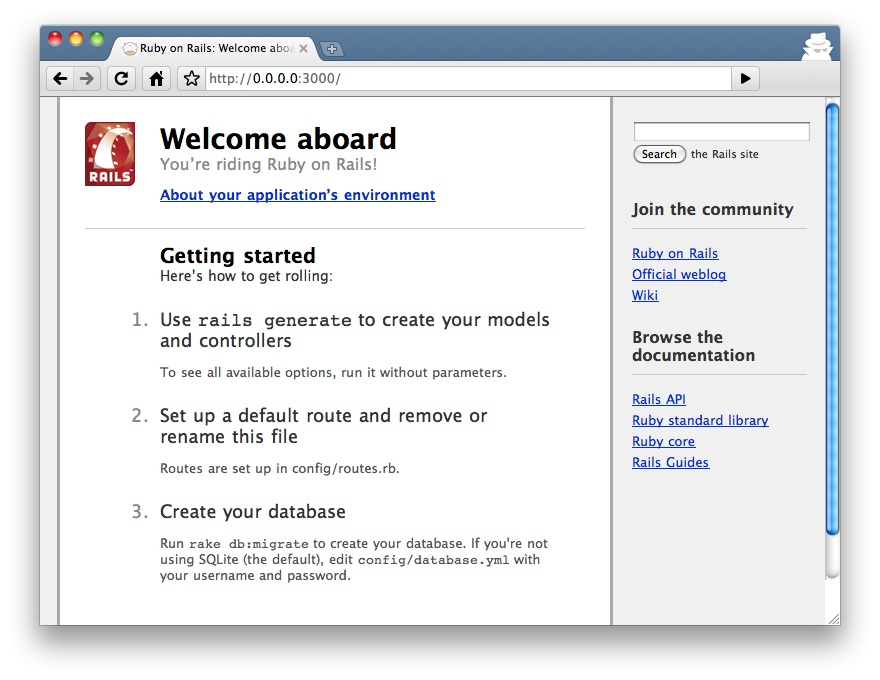
\includegraphics{screenshots/virgin_rails_app.jpg}
\end{figure}

Looks good. Rails seems to be working fine. The log of it tells what just happend:

\begin{shaded}\begin{verbatim}
Started GET "/" for 127.0.0.1 at 2013-07-15 13:59:35 +0200
Processing by Rails::WelcomeController#index as HTML
  Rendered /Users/xyz/.rvm/gems/ruby-2.0.0-p247/gems/railties-4.0.0/lib/rails/templates/rails/welcome/index.html.erb (1.1ms)
Completed 200 OK in 21ms (Views: 5.3ms | ActiveRecord: 0.0ms)
\end{verbatim}\end{shaded}

If we now click the link “\emph{About your application's environment}”, we can more information on the current environment.

\subsection{Important}\label{important-3}

With \textbf{Ctrl}+\textbf{C} you can stop the web server.

\section{Static Pages}\label{static-pages}

There are certain static pages, images and JavaScript files that are automatically output by Rails. Remember part of the output of the command \textbf{rails new testproject}:

\begin{shaded}\begin{verbatim}
$ rails new testproject
      [...]
      create  public/404.html
      create  public/422.html
      create  public/500.html
      create  public/favicon.ico
      create  public/robots.txt
      [...]
\end{verbatim}\end{shaded}

The directory name \texttt{public} and the files it contains already look very much like static pages. Let's have a go and create the file \texttt{public/hello-world.html} with the following content:

\begin{shaded}\begin{verbatim}
<html>
<head>
  <title>Hello World!</title>
</head>
<body>
  <h1>Hello World!</h1>
  <p>An example page.</p>
</body>
</html>
\end{verbatim}\end{shaded}

Now start the Rails web server with \textbf{rails server}

\begin{shaded}\begin{verbatim}
$ rails server
=> Booting WEBrick
=> Rails 4.0.0 application starting in development on http://0.0.0.0:3000
=> Run `rails server -h` for more startup options
=> Ctrl-C to shutdown server
[2013-07-15 14:05:57] INFO  WEBrick 1.3.1
[2013-07-15 14:05:57] INFO  ruby 2.0.0 (2013-06-27) [x86_64-darwin12.4.0]
[2013-07-15 14:05:57] INFO  WEBrick::HTTPServer#start: pid=98564 port=3000
\end{verbatim}\end{shaded}

We can have a look at this web page at the URL \texttt{http://0.0.0.0:3000/hello-world}:

\begin{figure}[htbp]
\centering
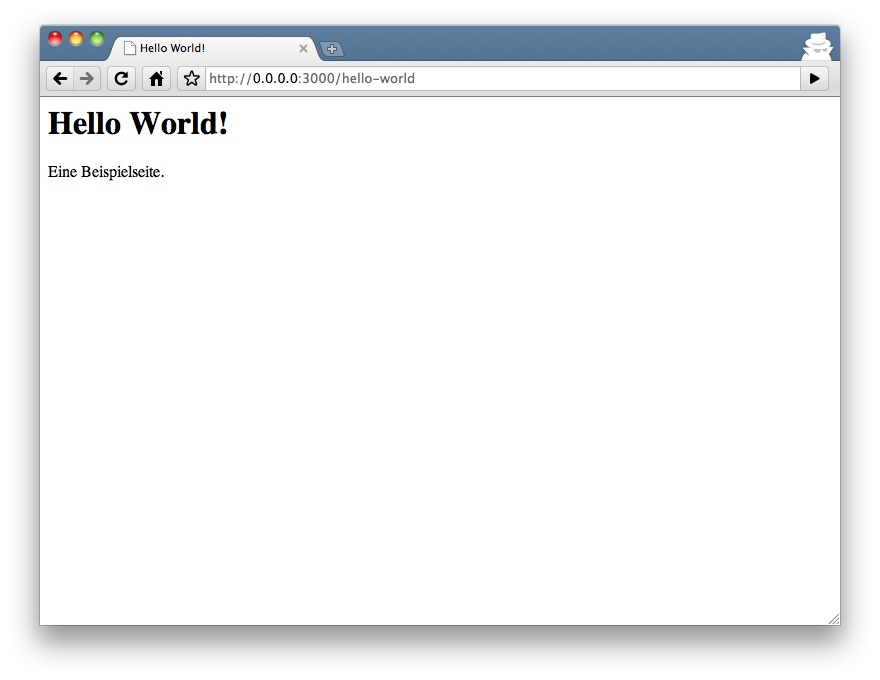
\includegraphics{screenshots/hello-world-html.jpg}
\end{figure}

No output in the log means: This page was not handled by the Rails framework. It was delivered directly from the webserver.

\section{Note}\label{note-14}

We can of course also use the URL \texttt{http://0.0.0.0:3000/hello-world.html}. But Rails regards HTML and therefore the file ending \texttt{.html} as standard output format, so you can omit the “\texttt{.html}” here.

Now you know how you can integrate fully static pages in Rails. This is useful for pages that never change and that you want to work even if Rails is not currently working, for example because of an update. In a production environment, you would usually put a classic web server such as Apache or Nginx infront of the Rails server. Which is capable of autonomously delivering static files from the \texttt{public} directory. You'll learn how to set up a production webserver in \hyperref[railsux5fproductionux5fwebserver]{Chapter~16, \emph{Web Server in Production Mode}}.

With \textbf{Ctrl}+\textbf{C} you can stop the Rails server.

\chap{Creating HTML Dynamically with erb}\label{creating-html-dynamically-with-erb}

The the content of an \texttt{erb} file will propably seem familiar to you. It is a mixture of HTML and Ruby code (\texttt{erb} stands for \emph{\textbf{e}mbedded \textbf{R}u\textbf{b}y}). erb pages are rendered as Views. This is the first time for us to get in touch with the MVC model.\textsuperscript{{[}\hyperref[ftn.idp1456352]{7}{]}} We need a controller to use a view. That can be created it via the generator \textbf{rails generate controller}. Let's have a look at the onboard help of this generator:

\begin{shaded}\begin{verbatim}
$ rails generate controller
Usage:
  rails generate controller NAME [action action] [options]

Options:
      [--skip-namespace]        # Skip namespace (affects only isolated applications)
  -e, [--template-engine=NAME]  # Template engine to be invoked
                                # Default: erb
  -t, [--test-framework=NAME]   # Test framework to be invoked
                                # Default: test_unit
      [--helper]                # Indicates when to generate helper
                                # Default: true
      [--assets]                # Indicates when to generate assets
                                # Default: true

Runtime options:
  -f, [--force]    # Overwrite files that already exist
  -p, [--pretend]  # Run but do not make any changes
  -q, [--quiet]    # Suppress status output
  -s, [--skip]     # Skip files that already exist

Description:
    Stubs out a new controller and its views. Pass the controller name, either
    CamelCased or under_scored, and a list of views as arguments.

    To create a controller within a module, specify the controller name as a
    path like 'parent_module/controller_name'.

    This generates a controller class in app/controllers and invokes helper,
    template engine, assets, and test framework generators.

Example:
    `rails generate controller CreditCards open debit credit close`

    CreditCards controller with URLs like /credit_cards/debit.
        Controller: app/controllers/credit_cards_controller.rb
        Test:       test/controllers/credit_cards_controller_test.rb
        Views:      app/views/credit_cards/debit.html.erb [...]
        Helper:     app/helpers/credit_cards_helper.rb
$
\end{verbatim}\end{shaded}

Nice! We are kindly provided with an example further down:

\begin{shaded}\begin{verbatim}
rails generate controller CreditCard open debit credit close
\end{verbatim}\end{shaded}

Doesn't really fit the bill for our case but I am feeling brave and suggest that we simply try \textbf{rails generate controller Example test}

\begin{shaded}\begin{verbatim}
$ rails generate controller Example test
      create  app/controllers/example_controller.rb
       route  get "example/test"
      invoke  erb
      create    app/views/example
      create    app/views/example/test.html.erb
      invoke  test_unit
      create    test/controllers/example_controller_test.rb
      invoke  helper
      create    app/helpers/example_helper.rb
      invoke    test_unit
      create      test/helpers/example_helper_test.rb
      invoke  assets
      invoke    coffee
      create      app/assets/javascripts/example.js.coffee
      invoke    scss
      create      app/assets/stylesheets/example.css.scss
$
\end{verbatim}\end{shaded}

Phew\ldots{} that's a lot of stuff being created. Amongst others, the file \texttt{app/views/example/test.html.erb}. Let's have a closer look at it:

\begin{shaded}\begin{verbatim}
$ cat app/views/example/test.html.erb
<h1>Example#test</h1>
<p>Find me in app/views/example/test.html.erb</p>
$
\end{verbatim}\end{shaded}

It's HTML, but for it to be a valid HTML page, something is “missing” at the top and bottom (the missing HTML “rest” will be explained in \hyperref[erbux5flayouts]{the section called “Layouts”}). We launch the web server to test it

\begin{shaded}\begin{verbatim}
$ rails server
\end{verbatim}\end{shaded}

and have a look at the web page in the browser at the URL \texttt{http://0.0.0.0:3000/example/test}:

\begin{figure}[htbp]
\centering
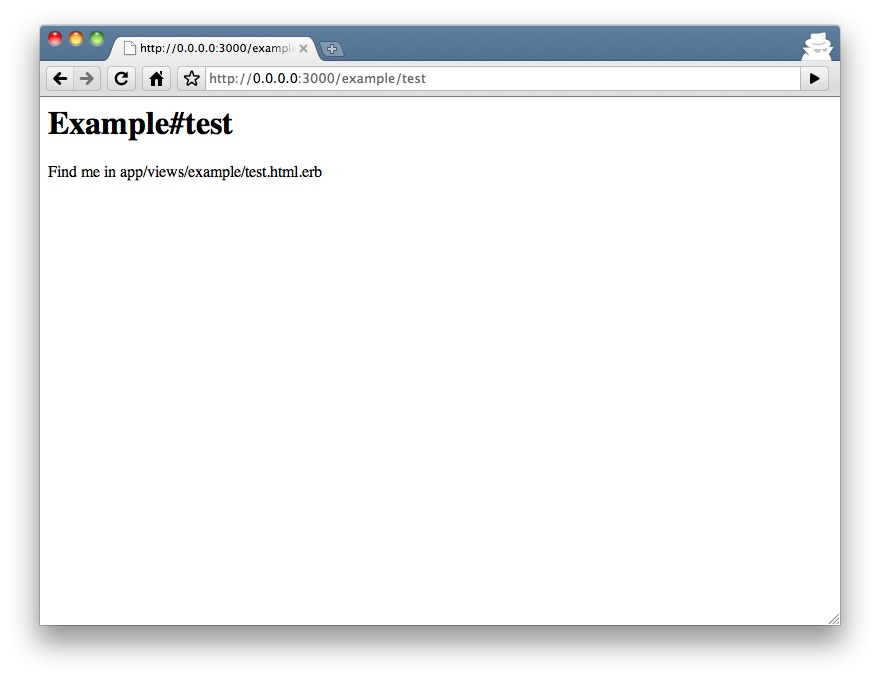
\includegraphics{screenshots/example-test-erb.jpg}
\end{figure}

In the log \texttt{log/development.log} we find the following lines:

\begin{shaded}\begin{verbatim}
Started GET "/example/test" for 127.0.0.1 at 2013-07-15 14:32:07 +0200
Processing by ExampleController#test as HTML
  Rendered example/test.html.erb within layouts/application (0.8ms)
Completed 200 OK in 768ms (Views: 751.0ms | ActiveRecord: 0.0ms)

Started GET "/assets/example.css?body=1" for 127.0.0.1 at 2013-07-15 14:32:08 +0200
Started GET "/assets/example.js?body=1" for 127.0.0.1 at 2013-07-15 14:32:08 +0200
Started GET "/assets/application.css?body=1" for 127.0.0.1 at 2013-07-15 14:32:08 +0200
Started GET "/assets/jquery_ujs.js?body=1" for 127.0.0.1 at 2013-07-15 14:32:08 +0200
Started GET "/assets/jquery.js?body=1" for 127.0.0.1 at 2013-07-15 14:32:08 +0200
Started GET "/assets/application.js?body=1" for 127.0.0.1 at 2013-07-15 14:32:08 +0200
Started GET "/assets/turbolinks.js?body=1" for 127.0.0.1 at 2013-07-15 14:32:08 +0200
\end{verbatim}\end{shaded}

That almost reads like normal English. Let us analyse the first part:

\begin{shaded}\begin{verbatim}
Started GET "/example/test" for 127.0.0.1 at 2013-07-15 14:32:07 +0200
Processing by ExampleController#test as HTML
  Rendered example/test.html.erb within layouts/application (0.8ms)
\end{verbatim}\end{shaded}

\texttt{localhost} (127.0.0.1) sent in an HTTP GET request for the URI “\texttt{/example/test}”. That was then apparently rendered as HTML by the controller \texttt{ExampleController} using the method \texttt{test}.

\section{Note}\label{note-15}

The other lines tell us that a bunch of CSS and JavaScript files are compiled and than delivered. In production mode these would be precompiled and delivered as one CSS and one J

Now we just need to find the controller. Good thing you bough this book. ;-) All controllers are in the directory \texttt{app/controllers}, and there you go, we indeed find the corresponding file \texttt{app/controllers/example\_controller.rb.}

\begin{shaded}\begin{verbatim}
$ ls -l app/controllers/
total 16
-rw-r-r--  1 xyz  staff  204 15 Jul 13:56 application_controller.rb
drwxr-xr-x  3 xyz  staff  102 15 Jul 13:56 concerns
-rw-r-r--  1 xyz  staff   69 15 Jul 14:31 example_controller.rb
$
\end{verbatim}\end{shaded}

Please open the file \texttt{app/controllers/example\_controller.rb} with your favorite editor:

\begin{shaded}\begin{verbatim}
class ExampleController < ApplicationController
  def test
  end
end
\end{verbatim}\end{shaded}

That is very clear. The controller \texttt{ExampleController} is a descendant of the \texttt{ApplicationController} and contains currently just one method with the name \texttt{test}. This method contains currently no program logic.

You will probably ask yourself how Rails knows that for the URL path \texttt{/example/test} it should process the controller \texttt{ExampleController} and the method \texttt{test}. This is not determined by some magical logic, but by a \emph{routing} configuration. The current routings can be listed with the command \textbf{rake routes}

\begin{shaded}\begin{verbatim}
$ rake routes
      Prefix Verb URI Pattern             Controller#Action
example_test GET /example/test(.:format) example#test
$
\end{verbatim}\end{shaded}

These routes are configured in the file \texttt{config/routes.rb} which has been auto-filled by the controller generator with a route to \texttt{example/test}. The one line which is important for us right now is the second one:

\begin{shaded}\begin{verbatim}
$ head -n 2 config/routes.rb
Testproject::Application.routes.draw do
  get "example/test"
$
\end{verbatim}\end{shaded}

The \texttt{config/routes.rb} file includes a lot of examples. Give it a read when you have time. We'll dive into that later (\hyperref[routes]{Chapter~6, \emph{Routes}}).

\subsection{Important}\label{important-4}

A static file in the directory \texttt{public} always has higher priority than a route in the \texttt{config/routes.rb}! So if we were to save a static file \texttt{public/example/test} that file will be delivered.

\section{Programming in an erb File}\label{programming-in-an-erb-file}

\texttt{Erb} pages can contain Ruby code. You can use it to program and give these page dynamic content.

Let's start with something very simple: adding 1 and 1. First we try out the code in \texttt{irb}:

\begin{shaded}\begin{verbatim}
$ irb --simple-prompt
>> 1 + 1
=> 2
>> exit
$
\end{verbatim}\end{shaded}

That was easy. We fill the \texttt{erb} file \texttt{app/views/example/test.html.erb} as follows:

\begin{shaded}\begin{verbatim}
<h1>First experiment with erb</h1>
<p>Addition:
<%= 1 + 1 %>
</p>
\end{verbatim}\end{shaded}

Then use \textbf{rails server} to launch the web server.

\begin{shaded}\begin{verbatim}
$ rails server
\end{verbatim}\end{shaded}

Visit that page with the URL \texttt{http://0.0.0.0:3000/example/test}

\begin{figure}[htbp]
\centering
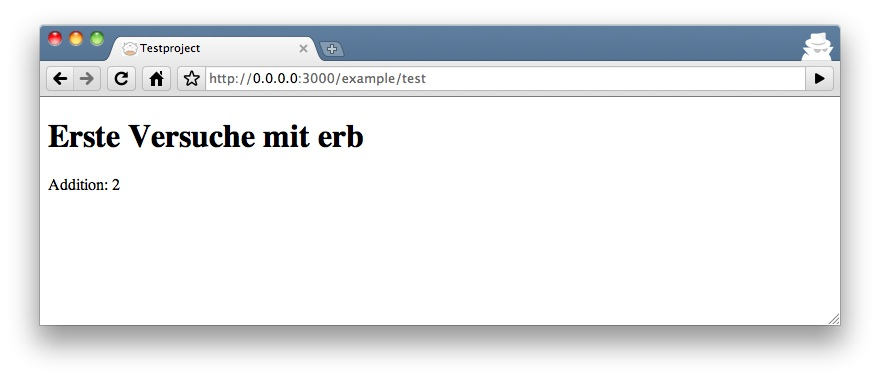
\includegraphics{screenshots/erb_einfache_addition.jpg}
\end{figure}

\section{Important}\label{important-5}

If you want to output the result of Ruby code, enclose the code within a \texttt{\textless{}\%=} \ldots{} \texttt{\%\textgreater{}}.

You may ask yourself: how can the result of adding two \texttt{Fixnums} be displayed as a String? Let's first look up in \texttt{irb} if it really is a \texttt{Fixnum}:

\begin{shaded}\begin{verbatim}
$ irb --simple-prompt
>> 1.class
=> Fixnum
>> (1 + 1).class
=> Fixnum
\end{verbatim}\end{shaded}

Yes, both the number 1 and the result of 1 + 1 is a \texttt{Fixnum}. What happened? Rails is so intelligent that it automatically calls all objects in a view (that is the file \texttt{test.html.erb}) that are not already a string via the method \texttt{.to\_s}, which always converts the content of the object to a string (\hyperref[ruby-toux5fs]{the section called “Method to\_s for Your Own Classes”}). Once more, a brief trip to \texttt{irb}:

\begin{shaded}\begin{verbatim}
>> (1 + 1).to_s
=> "2"
>> (1 + 1).to_s.class
=> String
>> exit
$
\end{verbatim}\end{shaded}

You are now going to learn the finer points of \texttt{erb} step by step. Don't worry, it's neither magic nor rocket science.

\section{\textless{}\% \ldots{} \%\textgreater{} vs. \textless{}\%= \ldots{} \%\textgreater{}}\label{vs.}

In a \texttt{.html.erb}file, there are two kinds of Ruby code instructions in addition to the HTML elements:

\begin{itemize}
\itemsep1pt\parskip0pt\parsep0pt
\item
  \textless{}\% \ldots{} \%\textgreater{} Executes the Ruby code it contains, but does not output anything (unless you explicitly use something like \texttt{print} or \texttt{puts}).
\item
  \textless{}\%= \ldots{} \%\textgreater{} Executes the Ruby code it contains and outputs the result as a String. If is is not a String the methode \texttt{to\_s} will be called.
\end{itemize}

\subsection{Important}\label{important-6}

The output of \textless{}\%= \ldots{} \%\textgreater{} is automatically escaped. So you don't need to worry about “dangerous” HTML.

Let's use an example, to make sure it all makes sense. We use \texttt{each} to iterate through the \texttt{Range} \texttt{(0..5)}. Edit the \texttt{app/views/example/test.html.erb} as follows:

\begin{shaded}\begin{verbatim}
<p>Loop from 0 to 5:
<% (0..5).each do |i| %>
<%= "#{i}, " %>
<% end %>
</p>
\end{verbatim}\end{shaded}

Open this view In the browser:

\begin{figure}[htbp]
\centering
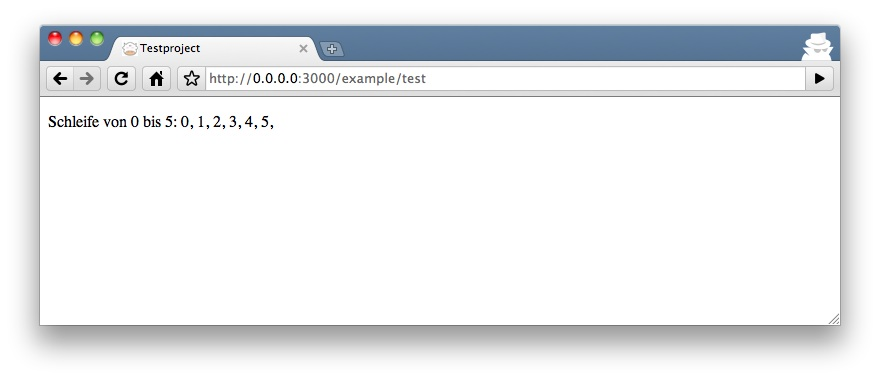
\includegraphics{screenshots/erb_einfache_schleife.jpg}
\end{figure}

Let's now have a look at the HTML source code in the browser:

\begin{shaded}\begin{verbatim}
<!DOCTYPE html>
<html>
<head>
  <title>Testproject</title>
  <link data-turbolinks-track="true" href="/assets/application.css?body=1" media="all" rel="stylesheet" />
<link data-turbolinks-track="true" href="/assets/example.css?body=1" media="all" rel="stylesheet" />
  <script data-turbolinks-track="true" src="/assets/jquery.js?body=1"></script>
<script data-turbolinks-track="true" src="/assets/jquery_ujs.js?body=1"></script>
<script data-turbolinks-track="true" src="/assets/turbolinks.js?body=1"></script>
<script data-turbolinks-track="true" src="/assets/example.js?body=1"></script>
<script data-turbolinks-track="true" src="/assets/application.js?body=1"></script>
  <meta content="authenticity_token" name="csrf-param" />
<meta content="FjIAd8nQGbKSAdbXdY47d3dhW1ZNLhe4eWJYYOgVdes=" name="csrf-token" />
</head>
<body>

<p>Loop from 0 to 5:
  0,
  1,
  2,
  3,
  4,
  5,
</p>


</body>
</html>
\end{verbatim}\end{shaded}

Now you have the important tools to use Ruby code in a view.

\chap{Q \& A}\label{q-a}

Potentially, there are two open questions:

\textbf{Q:}

I don't understand anything. I can't cope with the Ruby code. Could you please explain that again?

\textbf{A:}

Is it possible that you have not completely worked your way through \hyperref[ruby-grundlagen]{Chapter~2, \emph{Ruby Basics}}? Please do take your time with it and have another thorough look. Otherwise, the rest won't make any sense here.

\textbf{Q:}

I can understand the Ruby code and the HTML output. But I don't get why some HTML code was rendered around it if I didn't even write that HTML code. Where does it come from, and can I influence it?

\textbf{A:}

Excellent question! We will get to that next (see \hyperref[erbux5flayouts]{the section called “Layouts”}).

\chap{Layouts}\label{layouts}

The \texttt{erb} file in the directory \texttt{app/views/example/} only forms the core of the later HTML page. By default, an automatically generated \texttt{app/views/layouts/application.html.erb} is always rendered around it. Let's have a closer look at it:

\begin{shaded}\begin{verbatim}
<!DOCTYPE html>
<html>
<head>
  <title>Testproject</title>
  <%= stylesheet_link_tag    "application", media: "all", "data-turbolinks-track" => true %>
  <%= javascript_include_tag "application", "data-turbolinks-track" => true %>
  <%= csrf_meta_tags %>
</head>
<body>

<%= yield %>

</body>
</html>
\end{verbatim}\end{shaded}

The interesting bit is the line

\begin{shaded}\begin{verbatim}
<%= yield %>
\end{verbatim}\end{shaded}

With \texttt{\textless{}\%= yield \%\textgreater{}} the View file is included here. The lines with the stylesheets, the JavaScript and the csrf\_meta\_tags can stay as they are for now. They integrate default CSS and JavaScript files. We'll have a look into that in \hyperref[assetux5fpipeline]{Chapter~12, \emph{Asset Pipeline}}. No need to bother with that right now.

The file \texttt{app/views/layouts/application.html.erb} enables you to determine the basic layout for the entire Rails application. If you want to enter a \texttt{\textless{}hr\textgreater{}} for each page and above it a text, then you can do this between the \texttt{\textless{}\%= yield \%\textgreater{}} and the \texttt{\textless{}body\textgreater{}} tag:

\begin{shaded}\begin{verbatim}
<!DOCTYPE html>
<html>
<head>
  <title>Testproject</title>
  <%= stylesheet_link_tag    "application", :media => "all" %>
  <%= javascript_include_tag "application" %>
  <%= csrf_meta_tags %>
</head>
<body>

<h1>My Header</h1>
<hr>

<%= yield %>

</body>
</html>
\end{verbatim}\end{shaded}

You can also create other layouts in the directory \texttt{app/views/layouts/} and apply these layouts depending on the relevant situation. But let's leave it for now. The important thing is that you understand the basic concept.

\chap{Passing Instance Variables from a Controller to a View}\label{passing-instance-variables-from-a-controller-to-a-view}

One of the cardinal sins in the MVC model\textsuperscript{{[}\hyperref[ftn.idp2617376]{8}{]}}is to put too much program logic into the view. That's more or less what used to be done frequently in PHP programming in the past. I'm guilty of having done it myself. But one of the aims of MVC is that any HTML designer can create a view without having to worry about the programming. Yeah, yeah, \ldots{} if only it was always that easy. But let's just play it through in our minds: if I have a value in the controller that I want to display in the view, then I need a mechanism for this. This is referred to as \emph{instance variable} and always starts with a \texttt{@}. If you are not 100 \% sure any more which variable has which \emph{scope}, then please have another quick look at \hyperref[scopeux5fvonux5fvariablen]{the section called “Scope of Variables”}.

In the following example, we insert an instance variable for the current time in the controller and then insert it in the view. So we are taking programming intelligence from the view to the controller.

The controller file \texttt{app/controllers/example\_controller.rb} looks like this:

\begin{shaded}\begin{verbatim}
class ExampleController < ApplicationController
  def test
    @current_time = Time.now
  end
end
\end{verbatim}\end{shaded}

In the view file \texttt{app/views/example/test.html.erb} we can then access this instance variable:

\begin{shaded}\begin{verbatim}
<p>
The current time is
<%= @current_time %>
</p>
\end{verbatim}\end{shaded}

With the controller and the view, we now have a clear separation of programming logic and presentation logic. So now we can automatically adjust the time in the controller in accordance with the user's time zone, without the designer of the page having to worry about it. As always, the method \texttt{to\_s} is automatically applied in the view.

I am well aware that no-one will now jump up from their chair and shout: “Thank you for enlightening me! From now on, I will only program neatly in accordance with MVC.” The above example is just the first small step in the right direction and shows how we can easily get values from the controller to the view with instance variables.

\hyperdef{}{partials}{\section{Partials}\label{partials}}

Even with small web projects, there are often elements that appear repeatedly, for example a \emph{footer} on the page with contact info or a menu. Rails gives us the option of encapsulate this HTML code in form of \emph{partials} and then integrating it within a view. A partial is also stored in the directory \texttt{app/views/example/}. But the file name must start with an underscore (\texttt{\_}).

As an example, we now add a mini footer to our page in a separate partial. Copy the following content into the new file \texttt{app/views/example/\_footer.html.erb}:

\begin{shaded}\begin{verbatim}
<hr>
<p>
Copyright 2009 - <%= Date.today.year %> the Easter Bunny.
</p>
\end{verbatim}\end{shaded}

\subsection{Note}\label{note-16}

Yes, this is not the MVC way of doing it. Date.today.year should be defined in the Controller. I'm glad that you caught this mistake. I made it to show the use of a partial.

We edit the file \texttt{app/views/example/test.html.erb} as follows and insert the partial via the command\texttt{render}:

\begin{shaded}\begin{verbatim}
<p>Loop from 0 to 5:
<% (0..5).each do |i| %>
<%= "#{i}, " %>
<% end %>
</p>

<%= render "footer" %>
\end{verbatim}\end{shaded}

So now we have the following files in the directory \texttt{app/views/example}:

\begin{shaded}\begin{verbatim}
$ ls app/views/example
_footer.html.erb
test.html.erb
$
\end{verbatim}\end{shaded}

The new web page now looks like this:

\begin{figure}[htbp]
\centering
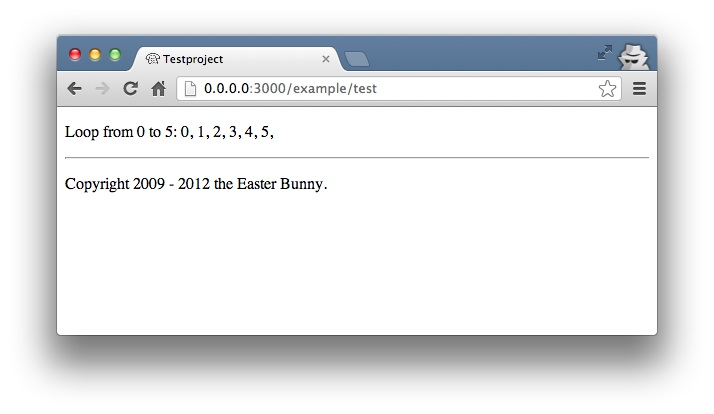
\includegraphics{screenshots/partials_footer.jpg}
\end{figure}

\subsection{Important}\label{important-7}

The name of a partial in the code is always specified \emph{without} the preceding underscore (\texttt{\_}) and \emph{without} the file extension \texttt{.erb} and \texttt{.html}. But the actual file must have the underscore at the beginning of the file name and end with the file extension \texttt{.erb} and \texttt{.html}.

Partials can also be integrated from other areas of the subdirectory \texttt{app/views}. For example, you can create a directory \texttt{app/views/shared} for recurring and shared content and create a file \texttt{\_footer.html.erb} in this directory. You would then integrate this file into the \texttt{erb} code via the line:

\begin{shaded}\begin{verbatim}
<%= render "shared/footer" %>
\end{verbatim}\end{shaded}

\section{Passing Variables to a Partial}\label{passing-variables-to-a-partial}

Partials are great in the sense of the DRY (\emph{\textbf{D}on't \textbf{R}epeat \textbf{Y}ourself}) concept. But what makes them really useful is the option of passing variables. Let's stick with the copyright example. If we want to pass the start year as value, we can integrate this by adding the following in the file \texttt{app/views/example/\_footer.html.erb}:

\begin{shaded}\begin{verbatim}
<hr>
<p>
Copyright <%= start_year %> - <%= Date.today.year %> the Easter Bunny.
</p>
\end{verbatim}\end{shaded}

So let's change the file \texttt{app/views/example/test.html.erb} as follows:

\begin{shaded}\begin{verbatim}
<p>Loop from 0 to 5:
<% (0..5).each do |i| %>
<%= "#{i}, " %>
<% end %>
</p>

<%= render "footer", :start_year => '2000' %>
\end{verbatim}\end{shaded}

If we now go to the URL \texttt{http://0.0.0.0:3000/example/test}, we see the 2000:

\begin{figure}[htbp]
\centering
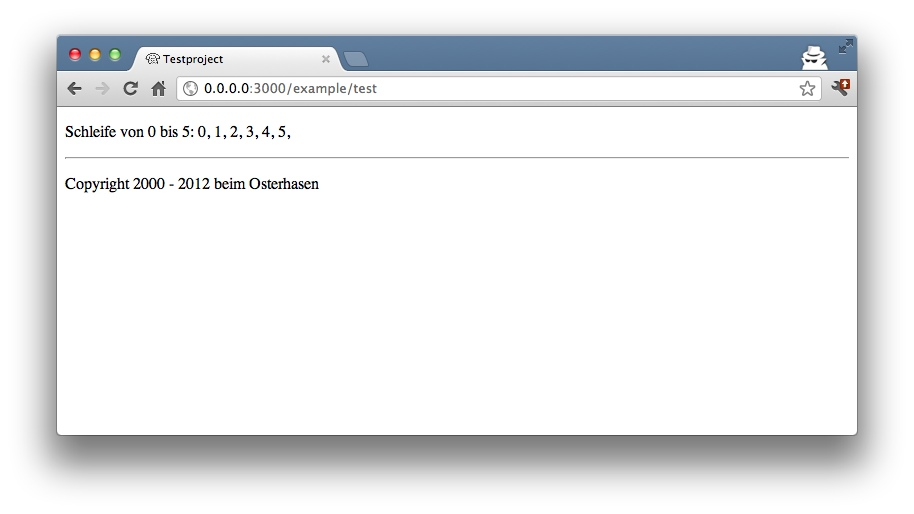
\includegraphics{screenshots/partial_start_year_2000.jpg}
\end{figure}

Sometimes you need a partial that partially uses a local variable and somewhere else you may need the same partial, but without the local variable. We can take care of this in the partial itself with an if statement:

\begin{shaded}\begin{verbatim}
<hr>
<p>
Copyright
<%= "#{start_year} - " if defined? start_year %>
<%= Date.today.year %>
the Easter Bunny.
</p>
\end{verbatim}\end{shaded}

\subsection{Note}\label{note-17}

\texttt{defined?} can be used to check if an expression has been defined.

You can call this partial with \texttt{\textless{}\%= render 'footer',         :start\_year =\textgreater{} '2000' \%\textgreater{}} and with \texttt{\textless{}\%= render         'footer' \%\textgreater{}}.

\section{Alternative Notation}\label{alternative-notation}

In \hyperref[partialsux5flocaleux5fvariables]{the section called “Passing Variables to a Partial”} we only use the short form for rendering partials. Often, you will also see this long version:

\begin{shaded}\begin{verbatim}
<%= render :partial => "footer", :locals => { :start_year => '2000' } %>
\end{verbatim}\end{shaded}

\chap{Further Documentation on Partials}\label{further-documentation-on-partials}

We have really only barely scratched the surface here. Partials are very powerful tools. You can find the official Ruby on Rails documentation on partials at \url{http://guides.rubyonrails.org/layouts_and_rendering.html\#using-partials}\{.uri\}.

\hyperdef{}{redirects}{\section{Redirects}\label{redirects}}

The name says it all, really: \emph{redirects} are commands that you can use within the controller to “skip”, i.e.~redirect, to other to other web pages.

\subsection{Note}\label{note-18}

A redirect returns to the browser the response “302 Moved” with the new target. So each redirect does a roundtrip to the browser and back.

Let's create a new Rails project for a suitable example:

\begin{shaded}\begin{verbatim}
$ rails new redirect_example
[...]
$ cd redirect_example
$
\end{verbatim}\end{shaded}

Before we can redirect, we need a controller with at least two different methods. Off we go then:

\begin{shaded}\begin{verbatim}
$ rails generate controller Game ping pong
      create  app/controllers/game_controller.rb
       route  get "game/pong"
       route  get "game/ping"
      invoke  erb
      create    app/views/game
      create    app/views/game/ping.html.erb
      create    app/views/game/pong.html.erb
      invoke  test_unit
      create    test/controllers/game_controller_test.rb
      invoke  helper
      create    app/helpers/game_helper.rb
      invoke    test_unit
      create      test/helpers/game_helper_test.rb
      invoke  assets
      invoke    coffee
      create      app/assets/javascripts/game.js.coffee
      invoke    scss
      create      app/assets/stylesheets/game.css.scss
$
\end{verbatim}\end{shaded}

The controller \texttt{app/controllers/game\_controller.rb} has the following content:

\begin{shaded}\begin{verbatim}
class GameController < ApplicationController
  def ping
  end

  def pong
  end
end
\end{verbatim}\end{shaded}

Now for the redirect: how can we achieve that we get immediately redirected to the method \texttt{pong} when we go to \texttt{http://0.0.0.0:3000/game/ping}? Easy, you will say, we just change the route in \texttt{config/routes.rb}. And you are right. So we don't necessarily need a redirect. But if we want to process something else in the method \texttt{ping} before redirecting, then this is only possible by using a \texttt{redirect\_to} in the controller \texttt{app/controllers/game\_controller.rb}:

\begin{shaded}\begin{verbatim}
class GameController < ApplicationController
  def ping
   logger.info '+++  Example  +++'
   redirect_to game_pong_path
  end

  def pong
  end
end
\end{verbatim}\end{shaded}

But what is \texttt{game\_pong\_path}? Let's have a look a the routes generated for this Rails application:

\begin{shaded}\begin{verbatim}
$ rake routes
   Prefix Verb URI Pattern          Controller#Action
game_ping GET /game/ping(.:format) game#ping
game_pong GET /game/pong(.:format) game#pong
$
\end{verbatim}\end{shaded}

\section{Note}\label{note-19}

As you can see, the route to the \emph{action}\texttt{ping} of the controller \texttt{GameController} now gets the name \texttt{game\_ping} (see beginning of the line). We could also write the redirect like this:

\begin{shaded}\begin{verbatim}
redirect_to :action => 'pong'
\end{verbatim}\end{shaded}

I will explain the details and the individual options of the redirect later in the context of each specific case. For now, you just need to know that you can redirect not just to another method, but also to another controller or an entirely different web page.

When we try to go to \texttt{http://0.0.0.0:3000/game/ping} we are automatically redirected to \texttt{http://0.0.0.0:3000/game/pong} and in the log output we see this:

\begin{shaded}\begin{verbatim}
Started GET "/game/ping" for 127.0.0.1 at 2013-07-15 18:49:01 +0200
Processing by GameController#ping as HTML
+++  Example  +++
Redirected to http://0.0.0.0:3000/game/pong
Completed 302 Found in 19ms (ActiveRecord: 0.0ms)


Started GET "/game/pong" for 127.0.0.1 at 2013-07-15 18:49:01 +0200
Processing by GameController#pong as HTML
  Rendered game/pong.html.erb within layouts/application (1.3ms)
Completed 200 OK in 743ms (Views: 741.9ms | ActiveRecord: 0.0ms)
\end{verbatim}\end{shaded}

\section{redirect\_to :back}\label{redirectux5fto-back}

If you want to redirect the user of your webapplication to the page he has just been you can use \texttt{redirect\_to :back}. This is very useful in a scenario where your user first has to login to get access to a specific page.

\section{Flash Messages}\label{flash-messages}

In my eyes, the term “\emph{flash messages}” is somewhat misleading. Almost anyone would associate the term “\emph{Flash}” with more or less colorful web pages that were implemented with the Adobe Shockwave Flash Plug-in. But in Ruby on Rails, flash messages are something completely different. They are messages that are displayed, for example on the new page after a redirect (see \hyperref[redirects]{the section called “Redirects”}).

Flash messages are good friends with redirects. The two often work together in a team to give the user feedback on an action he just carried out. A typical example of a flash message is the system feedback when a user has logged in. Often the user is redirected back to the original page and gets the message “You are now logged in.”

As an example, we are once more constructing the ping pong scenario from \hyperref[redirects]{the section called “Redirects”}:

\begin{shaded}\begin{verbatim}
$ rails new pingpong
      [...]
$ cd pingpong
$ rails generate controller Game ping pong
      [...]
$
\end{verbatim}\end{shaded}

We fill the \texttt{app/controllers/game\_controller.rb} with the following content:

\begin{shaded}\begin{verbatim}
class GameController < ApplicationController
  def ping
   redirect_to game_pong_path, notice: 'Ping-Pong!'
  end

  def pong
  end
end
\end{verbatim}\end{shaded}

Now we start the Rails web server with \textbf{rails server} and use the browser to go to \texttt{http://0.0.0.0:3000/game/ping}. We are redirected from \texttt{ping} to \texttt{pong}. But the flash message “Ping-Pong!” is nowhere to be seen. We first need to expand \texttt{app/views/layouts/application.html.erb}:

\begin{shaded}\begin{verbatim}
<html>
<head>
  <title>Pingpong</title>
  <%= stylesheet_link_tag    "application", media: "all", "data-turbolinks-track" => true %>
  <%= javascript_include_tag "application", "data-turbolinks-track" => true %>
  <%= csrf_meta_tags %>
</head>
<body>

<%- flash.each do |name, message| %>
<p><i><%= "#{name}: #{message}" %></i></p>
<% end %>

<%= yield %>

</body>
</html>
\end{verbatim}\end{shaded}

Now we see the flash message at the top of the page when we go to \texttt{http://0.0.0.0:3000/game/ping} in the browser:

\begin{figure}[htbp]
\centering
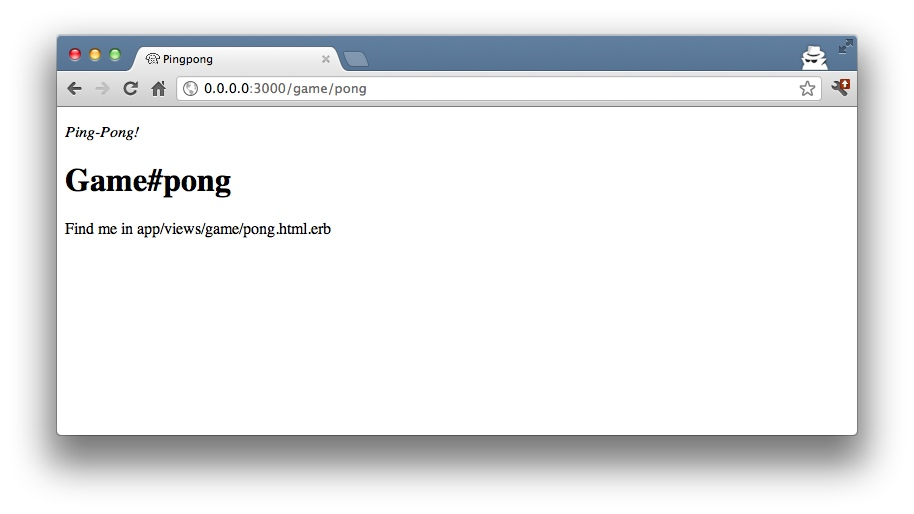
\includegraphics{screenshots/flash_pong_notice.jpg}
\end{figure}

If we go to \texttt{http://0.0.0.0:3000/game/pong} we still see the normal Pong page. But if we go to \texttt{http://0.0.0.0:3000/game/ping} we are redirected to the Pong page and then the flash message is displayed at the top.

\subsection{Tip}\label{tip-3}

If you do not see a flash message that you were expecting, first check in the view to see if the flash message is output there.

\section{Different Types of Flash Message}\label{different-types-of-flash-message}

Flash messages are automagically passed to the view in a hash. By default, there are three different types: \texttt{error}, \texttt{warning} and \texttt{notice}. You can also invent your own category and then get it in the view later.

\chap{Different Syntaxes}\label{different-syntaxes}

Depending on the programmer's preferences, you will find different syntaxes of flash messages in practice. I am not going to take part in the discussion about which is the best syntax, but just show you briefly the two most common variations:

\begin{itemize}
\item
  \texttt{\{.programlisting\}     redirect\_to game\_pong\_path, notice: 'Ping-Pong!'}
\item
  \texttt{\{.programlisting\}     flash{[}:notice{]} = 'Ping-Pong!'     redirect\_to action: pong}
\end{itemize}

Please have a look at the official documentation at \url{http://guides.rubyonrails.org/action_controller_overview.html\#the-flash}\{.uri\} for more information.

\section{Why Are There Flash Messages At All?}\label{why-are-there-flash-messages-at-all}

You may wonder why there are flash messages in the first place. Couldn't you just build them yourself if you need them? Yes, indeed. But flash messages have the advantage that they offer a defined approach that is the same for any programmer. So you don't need to start from scratch every single time you need one.

\section{The Rails Console}\label{the-rails-console}

The \emph{console} in Rails is nothing more than an \texttt{irb} (see \hyperref[irb]{the section called “irb”}) built around the Rails environment. The console is very useful both for developing and for administration purposes, because the whole Rails environment is represented and available.

For our working environment, we again use a variation of the ping pong scenario from \hyperref[redirects]{the section called “Redirects”}:

\begin{shaded}\begin{verbatim}
$ rails new pingpong
      [...]
$ cd pingpong
$ rails generate controller Game ping pong
      [...]
$
\end{verbatim}\end{shaded}

Start the Rails console with the command \textbf{rails console}:

\begin{shaded}\begin{verbatim}
$ rails console
Loading development environment (Rails 4.0.0)
2.0.0-p247 :001 >
\end{verbatim}\end{shaded}

And you can use \textbf{exit} to get back out:

\begin{shaded}\begin{verbatim}
2.0.0-p247 :001 > exit
$
\end{verbatim}\end{shaded}

Many readers use this document on mobile devises. For them I try to keep any code or terminal output width to a minimum. To save the real estate which is by default occupied by \texttt{2.0.0-p247 :001 \textgreater{}} we can start \textbf{rails console} with the parameter \emph{\texttt{-{}- -{}-simple-prompt}}.

\begin{shaded}\begin{verbatim}
$ rails console -- --simple-prompt
Loading development environment (Rails 4.0.0)
>> exit
$
\end{verbatim}\end{shaded}

Alternativly you can change the IRB configuration in the file \texttt{.irbrc} which is located in your home directory. If you want to have the simple prompt you have to add the following line in that file.

\begin{shaded}\begin{verbatim}
IRB.conf[:PROMPT_MODE] = :SIMPLE
\end{verbatim}\end{shaded}

In the console, you have access to all variables that are also available later in the proper application:

\begin{shaded}\begin{verbatim}
$ rails console
Loading development environment (Rails 4.0.0)
>> Rails.env
=> "development"
>> Rails.root
=> #<Pathname:/Users/xyz/pingpong>
>> exit
$
\end{verbatim}\end{shaded}

Already in \hyperref[activerecordux5fchapter]{Chapter~4, \emph{ActiveRecord}} we are going to be working lots with the console and will soon begin to appreciate the possibilities it offers.

\subsection{Tip}\label{tip-4}

One of my best buddies when developing Rails applications is the Tab key. Whenever you are looking for a method for a particular problem, recreate it in the Rails console and then press the Tab key twice to list all available methods. The names of the methods are usually self-exlanatory.

\section{app}\label{app}

\textbf{app} is useful if you want to analyze things to do with routing:

\begin{shaded}\begin{verbatim}
$ rails console
Loading development environment (Rails 4.0.0)
>> app.url_for(:controller => 'game', :action => 'ping')
=> "http://www.example.com/game/ping"
>> app.get 'game/ping'


Started GET "/game/ping" for 127.0.0.1 at 2013-07-15 19:19:36 +0200
Processing by GameController#ping as HTML
Redirected to http://www.example.com/game/pong
Completed 302 Found in 16ms (ActiveRecord: 0.0ms)
=> 302
>> app.get 'game/pong'


Started GET "/game/pong" for 127.0.0.1 at 2013-07-15 19:19:39 +0200
Processing by GameController#pong as HTML
  Rendered game/pong.html.erb within layouts/application (0.9ms)
Completed 200 OK in 50ms (Views: 49.2ms | ActiveRecord: 0.0ms)
=> 200
>> exit
$
\end{verbatim}\end{shaded}

\section{Misc}\label{misc}

You have now already created a simple Rails application and in the next chapter you will dive deeply into the topic ActiveRecord. So now is a good time to very briefly introduce a few terms that often surface in the world of Rails.

\section{“Model View Controller” Architecture (MVC)}\label{model-view-controller-architecture-mvc}

According to Wikipedia (\texttt{http://en.wikipedia.org/wiki/Model–view–controller}), MVC is a design pattern that separates the representation of information from the user's interaction with it.

MVC is a structure for software development. It was agreed that it makes sense to have one part of the software in one place and another part of the software in another place. Nothing more, nothing less. This agreement has the enormous advantage that once you are used to this concept, you know exactly where you can find or need to integrate a certain functionaity in a Rails project.

\chap{Model}\label{model}

“Model” in this case means data model. By default, Rails applications are an ActiveRecord data model (see \hyperref[activerecordux5fchapter]{Chapter~4, \emph{ActiveRecord}}).

All models can be found in the directory \texttt{app/models/.}

\section{View}\label{view}

The “view” is responsible for the presentation of the application. It takes care of rendering the web page, an XML or JSON file. A view could also render a PDF or an ASCII text. It depends entirely on your application.

You will find all the views in the directory \texttt{app/views/.}

\section{Controller}\label{controller}

Once a web page call has ended up in a route (see \hyperref[routes]{Chapter~6, \emph{Routes}}), it goes from there to the controller. The route specifies a certain method (action) as target. This method can then fulfil the desired tasks (such as finding a specific set of data and saving it in an instance variable) and then renders the desired view.

All controllers can be found in the directory \texttt{app/controllers/.}

\section{What is a Generator?}\label{what-is-a-generator}

We have already used the command \textbf{rails generate controller}. It starts the generator with the name \texttt{controller}. There are other generators as well. You can use the command \textbf{rails generate} to display a list of available generators:

\begin{shaded}\begin{verbatim}
$ rails generate
Usage: rails generate GENERATOR [args] [options]

General options:
  -h, [--help]     ## Print generator's options and usage
  -p, [--pretend]  # Run but do not make any changes
  -f, [--force]    # Overwrite files that already exist
  -s, [--skip]     # Skip files that already exist
  -q, [--quiet]    # Suppress status output

Please choose a generator below.

Rails:
  assets
  controller
  generator
  helper
  integration_test
  jbuilder
  mailer
  migration
  model
  resource
  scaffold
  scaffold_controller
  task

Coffee:
  coffee:assets

Jquery:
  jquery:install

Js:
  js:assets

TestUnit:
  test_unit:plugin

$
\end{verbatim}\end{shaded}

What does a generator do? A generator makes a programmer's job easier by doing some of the mindless tasks for you. It creates files and fills them with content, depending on the parameters passed. You could do the same manually, without the generator. So you do not have to use a generator. It is primarily intended to save you work and avoid potential errors that can easily arise from mindless repetitive tasks.

\subsection{Tip}\label{tip-5}

Someday you might want to create your own generator. Have a look at \url{http://guides.rubyonrails.org/generators.html}\{.uri\} to find a description of how to do that.

\section{Helper}\label{helper}

A helper method takes care of recurring tasks in a view. For example, if you want to display stars (*) for rating a restaurant and not a number from 1 to 5, you can define the following helper in the file \texttt{app/helpers/application\_helper.rb} :

\begin{shaded}\begin{verbatim}
module ApplicationHelper

  def render_stars(value)
    output = ''
    if (1..5).include?(value)
      value.times { output += '*'}
    end
    output
  end

end
\end{verbatim}\end{shaded}

With this helper, we can then apply the following code in a view:

\begin{shaded}\begin{verbatim}
<p>
<b>Rating:</b> <%= render_stars(5) %>
</p>
\end{verbatim}\end{shaded}

You can also try out the helper in the console:

\begin{shaded}\begin{verbatim}
$ rails console
Loading development environment (Rails 4.0.0)
>> helper.render_stars(5)
=> "*****"
>> helper.render_stars(3)
=> "***"
>> exit
$
\end{verbatim}\end{shaded}

There are lots of predefined helpers in Rails and we will use some of them in the next chapters. But you can also define your own custom helpers. Any of the helpers from the file \texttt{app/helpers/application\_helper.rb} can be used in any view. Helpers that you want to be only available in certain views must be defined for each controller. When creating a controller, a file for helpers of that controller is automatically created in \texttt{app/helpers}. This gives you the option of defining helpers only for this controller or for the views of this controller.

All helpers are in the directory \texttt{app/helpers/.}

\section{Rails Lingo}\label{rails-lingo}

Here you find a couple of words which you'll often find in the Ruby on Rails universe.

\section{DRY - Don't repeat yourself}\label{dry---dont-repeat-yourself}

Many Rails programmers are big fans of DRY. DRY means purely and simply that you should try to place repeated programming logic into separate methods.

\section{Refactoring}\label{refactoring}

You often hear the word refactoring in the context of DRY. This involves functioning applications that are further improved. The application in itself remains unchanged in its interface. But its core is optimized, amongst others through DRY.

\section{Convention Over Configuration}\label{convention-over-configuration}

Convention over configuration (also known as coding by convention, see \url{http://en.wikipedia.org/wiki/Convention_over_configuration}\{.uri\}) is an important pillar of a Rails application. It states that the programmer does not need to decide in favour of certain features when starting a project and set these via configuration parameters. It specifies an underlying basic consensus and this is set by default. But if you want to work outside of this conventional basic consensus, then you will need to change the corresponding parameters.

* * * * *

\textsuperscript{{[}\hyperref[idp1626704]{5}{]}}see \url{http://api.rubyonrails.org/classes/ActiveSupport/Inflector.html}\{.uri\}

\textsuperscript{{[}\hyperref[idp1628816]{6}{]}}see \url{http://en.wikipedia.org/wiki/Inflection}\{.uri\}

\textsuperscript{{[}\hyperref[idp1456352]{7}{]}}\url{http://en.wikipedia.org/wiki/Model-view-controller}\{.uri\}

\textsuperscript{{[}\hyperref[idp2617376]{8}{]}}\texttt{http://en.wikipedia.org/wiki/Model–view–controller}

\chap{ActiveRecord}\label{activerecord}

\texttt{ActiveRecord} is a level of abstraction that offers access to a SQL database. \texttt{ActiveRecord} implements the architectural pattern \emph{Active Record} \textsuperscript{{[}\hyperref[ftn.idp2940224]{9}{]}}.

\subsection{Note}\label{note-20}

This is referred to as \emph{object-relational mapping}, \emph{ORM}. I find it rather dry and boring, but in case you have trouble going to sleep tonight, have a look at \url{http://en.wikipedia.org/wiki/Object_relational_mapping}\{.uri\}.

One of the recipes for the success of Rails is surely the fact that is uses \texttt{ActiveRecord}. The programming and use “feels Ruby like” and it is much less susceptible to errors than pure SQL. When working with this chapter, it helps if you have some knowledge of SQL, but this is not required and also not essential for working with \texttt{ActiveRecord}.

Just as an aside, let me mention that you are not obliged to work with ActiveRecord when working with Rails. You can also use other ORMs. ActiveRecord is the default and is used by the majority of all Rails developers.

\section{Howto for this Chapter}\label{howto-for-this-chapter}

This chapter is a self-contained unit. But the knowledge provided in \hyperref[ruby-grundlagen]{Chapter~2, \emph{Ruby Basics}} and \hyperref[ersteux5fschritteux5fmitux5frails]{Chapter~3, \emph{First Steps with Rails}} is required. Without these basics, you will not have any fun with this chapter!

Rails newbies should read this chapter once from beginning to end. Please take your time. This chapter is important!

\section{Note}\label{note-21}

This chapter is only about ActiveRecord. So I am not going to integrate any tests (see \hyperref[testing]{Chapter~7, \emph{Tests}}), to keep the examples as simple as possible.

\section{Not in the Mood for SQL?}\label{not-in-the-mood-for-sql}

Occasionally, I will discuss SQL code created by ActiveRecord methods. If you are not interested in SQL: just read over it and don't worry. The beauty of ActiveRecord is that you do not need to think about it. For everyone else, my comments provide better understanding of the optimization processes going on in the background.

\section{Creating Database/“Model”}\label{creating-databasemodel}

\subsection{Note}\label{note-22}

\emph{Model} in this context refers to the data model of \emph{Model-View-Controller} (MVC).

As a first example, let's take a list of countries in Europe. First, we create a new Rails project:

\begin{shaded}\begin{verbatim}
$ rails new europe
  [...]
$ cd europe
$
\end{verbatim}\end{shaded}

Next, let's have a look at the help page for \textbf{rails generate model}:

\begin{shaded}\begin{verbatim}
$ rails generate model
Usage:
  rails generate model NAME [field[:type][:index] field[:type][:index]] [options]

Options:
      [--skip-namespace]  ## Skip namespace (affects only isolated applications)
  -o, --orm=NAME          # Orm to be invoked
                          # Default: active_record

ActiveRecord options:
      [--migration]            # Indicates when to generate migration
                               # Default: true
      [--timestamps]           # Indicates when to generate timestamps
                               # Default: true
      [--parent=PARENT]        # The parent class for the generated model
      [--indexes]              # Add indexes for references and belongs_to columns
                               # Default: true
  -t, [--test-framework=NAME]  # Test framework to be invoked
                               # Default: test_unit

TestUnit options:
      [--fixture]                   # Indicates when to generate fixture
                                    # Default: true
  -r, [--fixture-replacement=NAME]  # Fixture replacement to be invoked

Runtime options:
  -f, [--force]    # Overwrite files that already exist
  -p, [--pretend]  # Run but do not make any changes
  -q, [--quiet]    # Suppress status output
  -s, [--skip]     # Skip files that already exist

Description:
    Stubs out a new model. Pass the model name, either CamelCased or
    under_scored, and an optional list of attribute pairs as arguments.

    Attribute pairs are field:type arguments specifying the
    model's attributes. Timestamps are added by default, so you don't have to
    specify them by hand as 'created_at:datetime updated_at:datetime'.

    You don't have to think up every attribute up front, but it helps to
    sketch out a few so you can start working with the model immediately.

    This generator invokes your configured ORM and test framework, which
    defaults to ActiveRecord and TestUnit.

    Finally, if --parent option is given, it's used as superclass of the
    created model. This allows you create Single Table Inheritance models.

    If you pass a namespaced model name (e.g. admin/account or Admin::Account)
    then the generator will create a module with a table_name_prefix method
    to prefix the model's table name with the module name (e.g. admin_account)

Available field types:

    Just after the field name you can specify a type like text or boolean.
    It will generate the column with the associated SQL type. For instance:

        `rails generate model post title:string body:text`

    will generate a title column with a varchar type and a body column with a text
    type. You can use the following types:

        integer
        primary_key
        decimal
        float
        boolean
        binary
        string
        text
        date
        time
        datetime
        timestamp

    You can also consider `references` as a kind of type. For instance, if you run:

        `rails generate model photo title:string album:references`

    It will generate an album_id column. You should generate this kind of fields when
    you will use a `belongs_to` association for instance. `references` also support
    the polymorphism, you could enable the polymorphism like this:

        `rails generate model product supplier:references{polymorphic}`

    For integer, string, text and binary fields an integer in curly braces will
    be set as the limit:

        `rails generate model user pseudo:string{30}`

    For decimal two integers separated by a comma in curly braces will be used
    for precision and scale:

        `rails generate model product price:decimal{10,2}`

    You can add a `:uniq` or `:index` suffix for unique or standard indexes
    respectively:

        `rails generate model user pseudo:string:uniq`
        `rails generate model user pseudo:string:index`

    You can combine any single curly brace option with the index options:

        `rails generate model user username:string{30}:uniq`
        `rails generate model product supplier:references{polymorphic}:index`


Examples:
    `rails generate model account`

        For ActiveRecord and TestUnit it creates:

            Model:      app/models/account.rb
            Test:       test/models/account_test.rb
            Fixtures:   test/fixtures/accounts.yml
            Migration:  db/migrate/XXX_create_accounts.rb

    `rails generate model post title:string body:text published:boolean`

        Creates a Post model with a string title, text body, and published flag.

    `rails generate model admin/account`

        For ActiveRecord and TestUnit it creates:

            Module:     app/models/admin.rb
            Model:      app/models/admin/account.rb
            Test:       test/models/admin/account_test.rb
            Fixtures:   test/fixtures/admin/accounts.yml
            Migration:  db/migrate/XXX_create_admin_accounts.rb

$
\end{verbatim}\end{shaded}

The usage description \texttt{rails generate model NAME   {[}field{[}:type{]}{[}:index{]} field{[}:type{]}{[}:index{]}{]} {[}options{]}} tells us that after \texttt{rails generate model} comes the name of the model and then the table fields. If you do not put \texttt{:type} after a table field name, it is assumed to be a string by default. Let's create the \emph{model} \texttt{country}:

\begin{shaded}\begin{verbatim}
$ rails generate model Country name population:integer
      invoke  active_record
      create    db/migrate/20130715174248_create_countries.rb
      create    app/models/country.rb
      invoke    test_unit
      create      test/models/country_test.rb
      create      test/fixtures/countries.yml
$
\end{verbatim}\end{shaded}

The generator has created a database migration file with the name \texttt{db/migrate/20130715174248\_create\_countries.rb}. It provides the following code:

\begin{shaded}\begin{verbatim}
class CreateCountries < ActiveRecord::Migration
  def change
    create_table :countries do |t|
      t.string :name
      t.integer :population

      t.timestamps
    end
  end
end
\end{verbatim}\end{shaded}

A migration contains database changes. In this migration, a class \texttt{CreateCountries} is defined as a child of \texttt{ActiveRecord::Migration}. The class method \texttt{change} is used to define a migration and the associated roll-back.

With \textbf{rake db:migrate} we can apply the migrations, in other words, create the corresponding database table:

\begin{shaded}\begin{verbatim}
$ rake db:migrate
==  CreateCountries: migrating ================================================
-- create_table(:countries)
   -> 0.0010s
==  CreateCountries: migrated (0.0011s) =======================================

$
\end{verbatim}\end{shaded}

\section{Note}\label{note-23}

You will find more details on migrations in \hyperref[activerecordux5fmigration]{the section called “Migrations”}.

Let's have a look at the file \texttt{app/models/country.rb}:

\begin{shaded}\begin{verbatim}
class Country < ActiveRecord::Base
end
\end{verbatim}\end{shaded}

Hmmm \ldots{} the class \texttt{Country} is a child of \texttt{ActiveRecord::Base}. Makes sense, as we are discussing ActiveRecord in this chapter. ;-)

\section{The Attributes id, created\_at and updated\_at}\label{the-attributes-id-createdux5fat-and-updatedux5fat}

Even if you cannot see it in the migration, we also get the attributes \texttt{id}, \texttt{created\_at} und \texttt{updated\_at} by default for each ActiveRecord model. In the Rails console, we can output the attributes of the class \texttt{Country} by entering the class name:

\begin{shaded}\begin{verbatim}
$ rails console
Loading development environment (Rails 4.0.0)
>> Country
=> Country(id: integer, name: string, population: integer, created_at: datetime, updated_at: datetime)
>> exit
$
\end{verbatim}\end{shaded}

The attribute \texttt{created\_at} stores the time when the record was initially created. \texttt{updated\_at} shows the time of the last update for this record.

\texttt{id} is used a central identification of the record (primary key). The \texttt{id} is automatically incremented by 1 for each record.

\section{Getters and Setters}\label{getters-and-setters-1}

To read and write values of a SQL table row you can use by ActiveRecord provided getters and setters (\hyperref[rubyux5fgetterux5fandux5fsetter]{the section called “Getters and Setters”}). These attr\_accessors are automatically created. The getter of the field \texttt{updated\_at} for a given \texttt{Country} with the name \texttt{germany} would be \texttt{germany.updated\_at}.

\section{Possible Data Types in ActiveRecord}\label{possible-data-types-in-activerecord}

ActiveRecord is a \emph{layer} between Ruby and various relational databases. Unfortunately, many SQL databases have different perspectives regarding the definition of columns and their content. But you do not need to worry about this, because ActiveRecord solves this problem transparently for you.

\begin{itemize}
\itemsep1pt\parskip0pt\parsep0pt
\item
  Advantage: We can replace the database behind a Rails application without having to touch the program code.
\item
  Disadvantage: We cannot use all the features of the database concerned. We have to use the least common denominator, so to speak.
\end{itemize}

To generate a \emph{model}, you can use the following field types:

\begin{itemize}
\item
  \texttt{binary} This is a BLOB (\emph{Binary Large Object}) in the classical sense. Never heard of it? Then you probably won't need it. See also \url{http://en.wikipedia.org/wiki/Binary_large_object}\{.uri\}
\item
  \texttt{boolean} A Boolean value. Can be either \texttt{true} or \texttt{false}. See also \url{http://en.wikipedia.org/wiki/Boolean_data_type}\{.uri\}
\item
  \texttt{date} You can store a date here.
\item
  \texttt{datetime} Here you can store a date including a time.
\item
  \texttt{float} For storing a floating point number. See also \url{http://en.wikipedia.org/wiki/Floating_point}\{.uri\}
\item
  \texttt{integer} For storing an integer. See also \url{http://en.wikipedia.org/wiki/Integer_(computer_science)}\{.uri\}
\item
  \texttt{decimal}

  For storing a decimal number.

  \subsection{Tip}\label{tip-6}

  You can also enter a decimal directly with the model generator. But you need to observe the special syntax. Example for creating a price with a decimal:

\begin{shaded}\begin{verbatim}
$ rails generate model product name 'price:decimal{7,2}'
      invoke  active_record
      create    db/migrate/20121114110808_create_products.rb
      create    app/models/product.rb
      invoke    test_unit
      create      test/unit/product_test.rb
      create      test/fixtures/products.yml
$
\end{verbatim}\end{shaded}

  That would generate the following migration (\texttt{db/migrate/20121114110808\_create\_products.rb}):

\begin{shaded}\begin{verbatim}
class CreateProducts < ActiveRecord::Migration
  def change
    create_table :products do |t|
      t.string :name
      t.decimal :price, :precision => 7, :scale => 2

      t.timestamps
    end
  end
end
\end{verbatim}\end{shaded}
\item
  \texttt{primary\_key} This is an integer that is automatically incremented by 1 by the database for each new entry. This field type is often used as key for linking different database tables or \emph{models}. See also \url{http://en.wikipedia.org/wiki/Unique_key}\{.uri\}
\item
  \texttt{string} A string, in other words a sequence of any characters, up to a maximum of 2\textsuperscript{8}-1 (= 255) characters. See also \url{http://en.wikipedia.org/wiki/String_(computer_science)}\{.uri\}
\item
  \texttt{text} Also a string - but considerably bigger. By default, up to 2\textsuperscript{16} (=

  \begin{enumerate}
  \def\labelenumi{\arabic{enumi})}
  \setcounter{enumi}{65535}
  \itemsep1pt\parskip0pt\parsep0pt
  \item
    characters can be saved here.
  \end{enumerate}
\item
  \texttt{time} A time.
\item
  \texttt{timestamp} A time with date, filled in automatically by the database.
\end{itemize}

In \hyperref[activerecordux5fmigration]{the section called “Migrations”} we will provide more information on the individual data types and discuss available options. Don't forget, this is a book for beginners, so this section just gives a brief overview. If you want to find out more about the various datatypes, please refer to the documentation listed in \hyperref[weiterfuehrendeux5fdoku]{Appendix~A, \emph{Further Rails Documentation}}.

\chap{Naming Conventions (Country vs.~country vs.~countries)}\label{naming-conventions-country-vs.country-vs.countries}

Rails newbies often find it hard to figure out when to use upper and lower case, for example, \texttt{Country} or \texttt{country} (one is a class, the other one a model). The problem is usually not the class itself, but purely the spelling or wording. For now, let's just say: it's all very logical and you will quickly get the hang of it. The important thing is that you keep using English words, even if you would normally be programming in another language (see \hyperref[warumux5fenglish]{the section called “Why Is It All in English?”}).

Originally, my plan was to now start philosophizing at great length on naming conventions. But then I thought: “Jeez, the readers want to get going and not sit here for ages reading about theory.” So I am now going to introduce the methods with which you can find out the naming conventions yourself in the Rails \emph{console}:

\begin{shaded}\begin{verbatim}
$ rails console
Loading development environment (Rails 4.0.0)
>> 'country'.classify
=> "Country"
>> 'country'.tableize
=> "countries"
>> 'country'.foreign_key
=> "country_id"
>>
\end{verbatim}\end{shaded}

ActiveRecord automatically uses the English plural forms. So for the class \texttt{Country}, it's \texttt{countries}. If you are not sure about a term, you can also work with the class and method \texttt{name}.

\begin{shaded}\begin{verbatim}
>> Country.name.tableize
=> "countries"
>> Country.name.foreign_key
=> "country_id"
>> exit
$
\end{verbatim}\end{shaded}

You will find a complete list of the corresponding methods at \url{http://rails.rubyonrails.org/classes/ActiveSupport/CoreExtensions/String/Inflections.html}\{.uri xml:lang=“en” lang=“en”\}. But I would recommend that, for now, you just go with the flow. If you are not sure, you can find out the correct notation with the methods shown above.

\section{Database Configuration}\label{database-configuration}

Which database is used by default? Let's have a quick look at the configuration file for the database (\texttt{config/database.yml}):

\begin{shaded}\begin{verbatim}
## SQLite version 3.x
#   gem install sqlite3
##
##   Ensure the SQLite 3 gem is defined in your Gemfile
##   gem 'sqlite3'
development:
  adapter: sqlite3
  database: db/development.sqlite3
  pool: 5
  timeout: 5000

## Warning: The database defined as "test" will be erased and
## re-generated from your development database when you run "rake".
## Do not set this db to the same as development or production.
test:
  adapter: sqlite3
  database: db/test.sqlite3
  pool: 5
  timeout: 5000

production:
  adapter: sqlite3
  database: db/production.sqlite3
  pool: 5
  timeout: 5000
\end{verbatim}\end{shaded}

As we are working in \texttt{development} mode, Rails has created a new SQLite3 database \texttt{db/development.sqlite3} as a result of \textbf{rake db:migrate} and saved all data there.

Fans of command line clients can use \texttt{sqlite3} for viewing this database:

\begin{shaded}\begin{verbatim}
$ sqlite3 db/development.sqlite3
SQLite version 3.7.12 2012-04-03 19:43:07
Enter ".help" for instructions
Enter SQL statements terminated with a ";"
sqlite> .tables
countries          schema_migrations
sqlite> .schema countries
CREATE TABLE "countries" ("id" INTEGER PRIMARY KEY AUTOINCREMENT NOT NULL, "name" varchar(255), "population" integer, "created_at" datetime, "updated_at" datetime);
sqlite> .exit
$
\end{verbatim}\end{shaded}

\section{Adding Records}\label{adding-records}

Actually, I would like to show you first how to view records, but there we have another chicken and egg problem. So first, here is how you can create a new record with \texttt{ActiveRecord}.

\section{create}\label{create}

The most frequently used method for creating a new record is \texttt{create}. Let's try creating a country in the console with the command \textbf{Country.create(name: `Germany', population: 81831000)}

\begin{shaded}\begin{verbatim}
$ rails console
Loading development environment (Rails 4.0.0)
>> Country.create(name: 'Germany', population: 81831000)
   (0.1ms)  begin transaction
  SQL (5.8ms)  INSERT INTO "countries" ("created_at", "name", "population", "updated_at") VALUES (?, ?, ?, ?)  [["created_at", Mon, 15 Jul 2013 17:58:19 UTC +00:00], ["name", "Germany"], ["population", 81831000], ["updated_at", Mon, 15 Jul 2013 17:58:19 UTC +00:00]]
   (1.0ms)  commit transaction
=> #<Country id: 1, name: "Germany", population: 81831000, created_at: "2013-07-15 17:58:19", updated_at: "2013-07-15 17:58:19">
>> exit
$
\end{verbatim}\end{shaded}

ActiveRecord saves the new record and outputs the executed SQL command in the development environment. But to make absolutely sure it works, let's have a quick look with the command line client \texttt{sqlite3}:

\begin{shaded}\begin{verbatim}
$ sqlite3 db/development.sqlite3
SQLite version 3.7.12 2012-04-03 19:43:07
Enter ".help" for instructions
Enter SQL statements terminated with a ";"
sqlite> SELECT * FROM countries;
1|Germany|81831000|2013-07-15 17:58:19.600948|2013-07-15 17:58:19.600948
sqlite> .exit
$
\end{verbatim}\end{shaded}

\section{Syntax}\label{syntax}

The method \texttt{create} can handle a number of different syntax constructs. If you want to create a single record, you can do this with or without \{\}-brackets within the the ()-brackets:

\begin{itemize}
\itemsep1pt\parskip0pt\parsep0pt
\item
  \texttt{Country.create(name: 'Germany', population:             81831000)}
\item
  \texttt{Country.create(\{name: 'Germany', population:             81831000\})}
\end{itemize}

Similarly, you can describe the attributes differently:

\begin{itemize}
\itemsep1pt\parskip0pt\parsep0pt
\item
  \texttt{Country.create(:name =\textgreater{} 'Germany', :population             =\textgreater{} 81831000)}
\item
  \texttt{Country.create('name' =\textgreater{} 'Germany', 'population'             =\textgreater{} 81831000)}
\item
  \texttt{Country.create( name: 'Germany', population: 81831000             )}
\end{itemize}

You can also pass an array of hashes to \texttt{create} and use this approach to create several records at once:

\begin{shaded}\begin{verbatim}
Country.create([{name: 'Germany'}, {name: 'France'}])
\end{verbatim}\end{shaded}

\section{new}\label{new}

In addition to \texttt{create} there is also \texttt{new}. But you have to use \texttt{save} to save an object created with \texttt{new} (which has both advantages and disadvantages):

\begin{shaded}\begin{verbatim}
$ rails console
Loading development environment (Rails 4.0.0)
>> france = Country.new
=> #<Country id: nil, name: nil, population: nil, created_at: nil, updated_at: nil>
>> france.name = 'France'
=> "France"
>> france.population = 65447374
=> 65447374
>> france.save
   (0.2ms)  begin transaction
  SQL (2.3ms)  INSERT INTO "countries" ("created_at", "name", "population", "updated_at") VALUES (?, ?, ?, ?)  [["created_at", Mon, 15 Jul 2013 18:07:03 UTC +00:00], ["name", "France"], ["population", 65447374], ["updated_at", Mon, 15 Jul 2013 18:07:03 UTC +00:00]]
   (3.0ms)  commit transaction
=> true
>> france
=> #<Country id: 2, name: "France", population: 65447374, created_at: "2013-07-15 18:07:03", updated_at: "2013-07-15 18:07:03">
>>
\end{verbatim}\end{shaded}

You can also pass parameters for the new record directly to the method \texttt{new}, just as with \texttt{create}:

\begin{shaded}\begin{verbatim}
>> belgium = Country.new(name: 'Belgium', population: 10839905)
=> #<Country id: nil, name: "Belgium", population: 10839905, created_at: nil, updated_at: nil>
>> belgium.save
   (0.2ms)  begin transaction
  SQL (1.3ms)  INSERT INTO "countries" ("created_at", "name", "population", "updated_at") VALUES (?, ?, ?, ?)  [["created_at", Mon, 15 Jul 2013 18:08:07 UTC +00:00], ["name", "Belgium"], ["population", 10839905], ["updated_at", Mon, 15 Jul 2013 18:08:07 UTC +00:00]]
   (2.1ms)  commit transaction
=> true
>> exit
$
\end{verbatim}\end{shaded}

\chap{new\_record?}\label{newux5frecord}

With the method \texttt{new\_record?} you can find out if a record has already been saved or not. If a new object has been created with \texttt{new} and not yet been saved, then the result of \texttt{new\_record?} is \texttt{true}. After a \texttt{save} it is \texttt{false}.

Example:

\begin{shaded}\begin{verbatim}
$ rails console
Loading development environment (Rails 4.0.0)
>> netherlands = Country.new(name: 'Netherlands')
=> #<Country id: nil, name: "Netherlands", population: nil, created_at: nil, updated_at: nil>
>> netherlands.new_record?
=> true
>> netherlands.save
   (0.2ms)  begin transaction
  SQL (2.3ms)  INSERT INTO "countries" ("created_at", "name", "updated_at") VALUES (?, ?, ?)  [["created_at", Mon, 15 Jul 2013 18:08:52 UTC +00:00], ["name", "Netherlands"], ["updated_at", Mon, 15 Jul 2013 18:08:52 UTC +00:00]]
   (3.1ms)  commit transaction
=> true
>> netherlands.new_record?
=> false
>> exit
$
\end{verbatim}\end{shaded}

\section{Tip}\label{tip-7}

For already existing records, you can also check for changes with the method \texttt{changed?} (see \hyperref[activerecordux5fchanged]{the section called “changed?”}).

\chap{first, last and all}\label{first-last-and-all}

In certain cases, you may need the first record, or the last one, or perhaps even all records. Conveniently, there is a ready-made method for each case. Let's start with the easiest ones: \texttt{first} and \texttt{last}.

\begin{shaded}\begin{verbatim}
$ rails console
Loading development environment (Rails 4.0.0)
>> Country.first
  Country Load (0.1ms)  SELECT "countries".* FROM "countries" ORDER BY "countries"."id" ASC LIMIT 1
=> #<Country id: 1, name: "Germany", population: 81831000, created_at: "2013-07-15 18:03:20", updated_at: "2013-07-15 18:03:20">
>> Country.last
  Country Load (0.3ms)  SELECT "countries".* FROM "countries" ORDER BY "countries"."id" DESC LIMIT 1
=> #<Country id: 4, name: "Netherlands", population: nil, created_at: "2013-07-15 18:08:52", updated_at: "2013-07-15 18:08:52">
>>
\end{verbatim}\end{shaded}

And now all at once with \texttt{all}:

\begin{shaded}\begin{verbatim}
>> Country.all
  Country Load (0.2ms)  SELECT "countries".* FROM "countries"
=> #<ActiveRecord::Relation [#<Country id: 1, name: "Germany", population: 81831000, created_at: "2013-07-15 18:03:20", updated_at: "2013-07-15 18:03:20">, #<Country id: 2, name: "France", population: 65447374, created_at: "2013-07-15 18:07:03", updated_at: "2013-07-15 18:07:03">, #<Country id: 3, name: "Belgium", population: 10839905, created_at: "2013-07-15 18:08:07", updated_at: "2013-07-15 18:08:07">, #<Country id: 4, name: "Netherlands", population: nil, created_at: "2013-07-15 18:08:52", updated_at: "2013-07-15 18:08:52">]>
>>
\end{verbatim}\end{shaded}

But the objects created by \texttt{first}, \texttt{last} and \texttt{all} are different. \texttt{first} and \texttt{last} return an object of the class \texttt{Country} and \texttt{all} of course returns an array of such objects:

\begin{shaded}\begin{verbatim}
>> Country.first.class
  Country Load (0.3ms)  SELECT "countries".* FROM "countries" ORDER BY "countries"."id" ASC LIMIT 1
=> Country(id: integer, name: string, population: integer, created_at: datetime, updated_at: datetime)
>> Country.all.class
=> ActiveRecord::Relation::ActiveRecord_Relation_Country
>>
\end{verbatim}\end{shaded}

So \texttt{Country.first} is a \texttt{Country} which makes sense. But \texttt{Country.all} is something we haven't had yet. Let's use the console to get a better idea of it:

\begin{shaded}\begin{verbatim}
>> puts Country.all.to_yaml
  Country Load (0.4ms)  SELECT "countries".* FROM "countries"
---
- !ruby/object:Country
  attributes:
    id: 1
    name: Germany
    population: 81831000
    created_at: 2013-07-15 18:03:20.814776000 Z
    updated_at: 2013-07-15 18:03:20.814776000 Z
- !ruby/object:Country
  attributes:
    id: 2
    name: France
    population: 65447374
    created_at: 2013-07-15 18:07:03.227571000 Z
    updated_at: 2013-07-15 18:07:03.227571000 Z
- !ruby/object:Country
  attributes:
    id: 3
    name: Belgium
    population: 10839905
    created_at: 2013-07-15 18:08:07.125974000 Z
    updated_at: 2013-07-15 18:08:07.125974000 Z
- !ruby/object:Country
  attributes:
    id: 4
    name: Netherlands
    population:
    created_at: 2013-07-15 18:08:52.736007000 Z
    updated_at: 2013-07-15 18:08:52.736007000 Z
=> nil
>>
\end{verbatim}\end{shaded}

hmmm\ldots{} by using the \texttt{to\_yaml} method suddenly the database has work to do. The reason for this behavior is optimization. Let's assume that you want to chain a couple of methods. Than it might be better for ActiveRecord to wait till the very last second which it does. It only requests the data from the SQL database when it has to do it. Until than it stores the request in a \texttt{ActiveRecord::Relation}.

The result of \texttt{Country.all} is actually an \texttt{Array} of \texttt{Country}.

If \texttt{Country.all} returns an array, then we should also be able to use iterators (see \hyperref[iterator]{the section called “Iterators”} and \hyperref[arrayux5fiterator]{the section called “Iterator each”}), right? Yes, of course! That is the beauty of it. Here is a little experiment with \texttt{each}:

\begin{shaded}\begin{verbatim}
>> Country.all.each do |country|
?> puts country.name
>> end
  Country Load (0.3ms)  SELECT "countries".* FROM "countries"
Germany
France
Belgium
Netherlands
=> [#<Country id: 1, name: "Germany", population: 81831000, created_at: "2013-07-15 18:03:20", updated_at: "2013-07-15 18:03:20">, #<Country id: 2, name: "France", population: 65447374, created_at: "2013-07-15 18:07:03", updated_at: "2013-07-15 18:07:03">, #<Country id: 3, name: "Belgium", population: 10839905, created_at: "2013-07-15 18:08:07", updated_at: "2013-07-15 18:08:07">, #<Country id: 4, name: "Netherlands", population: nil, created_at: "2013-07-15 18:08:52", updated_at: "2013-07-15 18:08:52">]
>>
\end{verbatim}\end{shaded}

So can we also use \texttt{.all.first} as an alternative for \texttt{.first}? Yes, but it does not make much sense. Have a look for yourself:

\begin{shaded}\begin{verbatim}
>> Country.first
  Country Load (0.3ms)  SELECT "countries".* FROM "countries" ORDER BY "countries"."id" ASC LIMIT 1
=> #<Country id: 1, name: "Germany", population: 81831000, created_at: "2013-07-15 18:03:20", updated_at: "2013-07-15 18:03:20">
>> Country.all.first
  Country Load (0.4ms)  SELECT "countries".* FROM "countries" ORDER BY "countries"."id" ASC LIMIT 1
=> #<Country id: 1, name: "Germany", population: 81831000, created_at: "2013-07-15 18:03:20", updated_at: "2013-07-15 18:03:20">
>>
\end{verbatim}\end{shaded}

\texttt{Country.first} and \texttt{Country.all.first} result in exact the same SQL query.

\chap{Populating the Database with seeds.rb}\label{populating-the-database-with-seeds.rb}

With the file \texttt{db/seeds.rb}, the Rails gods have given us a way of feeding default values easily and quickly to a fresh installation. This is a normal Ruby program within the Rails environment. You have full access to all classes and methods of your application.

So you do not need to enter everything manually with \textbf{rails console} in order to make the records created in \hyperref[activerecordux5fcreate]{the section called “create”} available in a new Rails application, but you can simply use the following file \texttt{db/seeds.rb}:

\begin{shaded}\begin{verbatim}
Country.create(name: 'Germany', population: 81831000)
Country.create(name: 'France', population: 65447374)
Country.create(name: 'Belgium', population: 10839905)
Country.create(name: 'Netherlands', population: 16680000)
\end{verbatim}\end{shaded}

You then populate it with data via \textbf{rake db:seed}. To be on the safe side, you should always set up the database from scratch with \textbf{rake db:setup} in the context of this book and then automatically populate it with the file \texttt{db/seeds.rb}. Here is what is looks like:

\begin{shaded}\begin{verbatim}
$ rake db:setup
db/development.sqlite3 already exists
-- create_table("countries", {:force=>true})
   -> 0.0101s
-- create_table("products", {:force=>true})
   -> 0.0030s
-- initialize_schema_migrations_table()
   -> 0.0010s
$
\end{verbatim}\end{shaded}

I use the file \texttt{db/seeds.rb} at this point because it offers a simple mechanism for filling an empty database with default values. In the course of this book, this will make it easier for us to set up quick example scenarios.

\section{It's all just Ruby code}\label{its-all-just-ruby-code}

The \texttt{db/seeds.rb} is a Ruby program. Correspondingly, we can also use the following approach as an alternative:

\begin{shaded}\begin{verbatim}
country_list = [
  [ "Germany", 81831000 ],
  [ "France", 65447374 ],
  [ "Belgium", 10839905 ],
  [ "Netherlands", 16680000 ]
]

country_list.each do |name, population|
  Country.create( name: name, population: population )
end
\end{verbatim}\end{shaded}

The result is the same. I am showing you this example to make it clear that you can program completely normally within the file \texttt{db/seeds.rb}.

\section{Generating seeds.rb From Existing Data}\label{generating-seeds.rb-from-existing-data}

Sometimes it can be useful to export the current data pool of a Rails application into a \texttt{db/seeds.rb}. While writing this book, I encountered this problem in almost every chapter. Unfortunately, there is no standard approach for this. I am showing you what you can do in this case. There are other, more complex scenarios that can be derived from my approach.

We create our own little rake task for that. That can be done by creating the file \texttt{lib/tasks/export.rake} with the following content:

\begin{shaded}\begin{verbatim}
namespace :export do
  desc "Prints Country.all in a seeds.rb way."
  task :seeds_format => :environment do
    Country.order(:id).all.each do |country|
      puts "Country.create(#{country.serializable_hash.delete_if {|key, value| ['created_at','updated_at','id'].include?(key)}.to_s.gsub(/[{}]/,'')})"
    end
  end
end
\end{verbatim}\end{shaded}

Then you can call the corresponding rake task with the command \textbf{rake export:seeds\_format}:

\begin{shaded}\begin{verbatim}
$ rake export:seeds_format
Country.create("name"=>"Germany", "population"=>81831000)
Country.create("name"=>"France", "population"=>65447374)
Country.create("name"=>"Belgium", "population"=>10839905)
Country.create("name"=>"Netherlands", "population"=>16680000)
$
\end{verbatim}\end{shaded}

You can either expand this program so that the output is written directly into the \texttt{db/seeds.rb} or you can simply use the shell:

\begin{shaded}\begin{verbatim}
$ rake export:seeds_format > db/seeds.rb
$
\end{verbatim}\end{shaded}

\section{Searching and Finding with Queries}\label{searching-and-finding-with-queries}

The methods \texttt{first} and \texttt{all} are already quite nice, but usually you want to search for something specific with a query.

For describing queries, we create a new Rails project:

\begin{shaded}\begin{verbatim}
$ rails new jukebox
  [...]
$ cd jukebox
$ rails generate model Album name release_year:integer
  [...]
$ rake db:migrate
  [...]
$
\end{verbatim}\end{shaded}

For the examples uses here, use a \texttt{db/seeds.rb} with the following content:

\begin{shaded}\begin{verbatim}
Album.create(name: "Sgt. Pepper's Lonely Hearts Club Band", release_year: 1967)
Album.create(name: "Pet Sounds", release_year: 1966)
Album.create(name: "Revolver", release_year: 1966)
Album.create(name: "Highway 61 Revisited", release_year: 1965)
Album.create(name: "Rubber Soul", release_year: 1965)
Album.create(name: "What's Going On", release_year: 1971)
Album.create(name: "Exile on Main St.", release_year: 1972)
Album.create(name: "London Calling", release_year: 1979)
Album.create(name: "Blonde on Blonde", release_year: 1966)
Album.create(name: "The Beatles", release_year: 1968)
\end{verbatim}\end{shaded}

Then, set up the new database with \textbf{rake db:setup}:

\begin{shaded}\begin{verbatim}
$ rake db:setup
db/development.sqlite3 already exists
-- create_table("albums", {:force=>true})
   -> 0.0085s
-- initialize_schema_migrations_table()
   -> 0.0010s
$
\end{verbatim}\end{shaded}

\section{find}\label{find}

The simplest case is searching for a record via a primary key (by default, the \texttt{id} field in the database table). If I know the ID of an object (here: a record line), then I can search for the individual object or several objects at once via the ID:

\begin{shaded}\begin{verbatim}
$ rails console
Loading development environment (Rails 4.0.0)
>> Album.find(2)
  Album Load (1.7ms)  SELECT "albums".* FROM "albums" WHERE "albums"."id" = ? LIMIT 1  [["id", 2]]
=> #<Album id: 2, name: "Pet Sounds", release_year: 1966, created_at: "2013-07-15 18:59:50", updated_at: "2013-07-15 18:59:50">
>> Album.find([1,3,7])
  Album Load (0.4ms)  SELECT "albums".* FROM "albums" WHERE "albums"."id" IN (1, 3, 7)
=> [#<Album id: 1, name: "Sgt. Pepper's Lonely Hearts Club Band", release_year: 1967, created_at: "2013-07-15 18:59:50", updated_at: "2013-07-15 18:59:50">, #<Album id: 3, name: "Revolver", release_year: 1966, created_at: "2013-07-15 18:59:50", updated_at: "2013-07-15 18:59:50">, #<Album id: 7, name: "Exile on Main St.", release_year: 1972, created_at: "2013-07-15 18:59:50", updated_at: "2013-07-15 18:59:50">]
>>  
\end{verbatim}\end{shaded}

If you always want to have an array as result, you also always have to pass an array as parameter:

\begin{shaded}\begin{verbatim}
>> Album.find(5).class
  Album Load (0.4ms)  SELECT "albums".* FROM "albums" WHERE "albums"."id" = ? LIMIT 1  [["id", 5]]
=> Album(id: integer, name: string, release_year: integer, created_at: datetime, updated_at: datetime)
>> Album.find([5]).class
  Album Load (0.3ms)  SELECT "albums".* FROM "albums" WHERE "albums"."id" = ? LIMIT 1  [["id", 5]]
=> Array
>> exit
$
\end{verbatim}\end{shaded}

\section{Warning}\label{warning-1}

The method\texttt{find} generates an exception if the ID you are searching for does not have a record in the database. If in doubt, you should use \texttt{where} (see \hyperref[activerecordux5fwhere]{the section called “where”}).

\chap{where}\label{where}

With the method \texttt{where}, you can search for specific values in the database. Let's search for all albums from the year 1966:

\begin{shaded}\begin{verbatim}
$ rails console
Loading development environment (Rails 4.0.0)
>> Album.where(release_year: 1966)
  Album Load (0.1ms)  SELECT "albums".* FROM "albums" WHERE "albums"."release_year" = 1966
=> #<ActiveRecord::Relation [#<Album id: 2, name: "Pet Sounds", release_year: 1966, created_at: "2013-07-15 18:59:50", updated_at: "2013-07-15 18:59:50">, #<Album id: 3, name: "Revolver", release_year: 1966, created_at: "2013-07-15 18:59:50", updated_at: "2013-07-15 18:59:50">, #<Album id: 9, name: "Blonde on Blonde", release_year: 1966, created_at: "2013-07-15 18:59:50", updated_at: "2013-07-15 18:59:50">]>
>> Album.where(release_year: 1966).count
   (0.3ms)  SELECT COUNT(*) FROM "albums" WHERE "albums"."release_year" = 1966
=> 3
>>
\end{verbatim}\end{shaded}

You can also use \texttt{where} to search for \emph{ranges} (see \hyperref[rangeux5fclass]{the section called “Range”}):

\begin{shaded}\begin{verbatim}
>> Album.where(release_year: 1960..1966)
  Album Load (0.3ms)  SELECT "albums".* FROM "albums" WHERE ("albums"."release_year" BETWEEN 1960 AND 1966)
=> #<ActiveRecord::Relation [#<Album id: 2, name: "Pet Sounds", release_year: 1966, created_at: "2013-07-15 18:59:50", updated_at: "2013-07-15 18:59:50">, #<Album id: 3, name: "Revolver", release_year: 1966, created_at: "2013-07-15 18:59:50", updated_at: "2013-07-15 18:59:50">, #<Album id: 4, name: "Highway 61 Revisited", release_year: 1965, created_at: "2013-07-15 18:59:50", updated_at: "2013-07-15 18:59:50">, #<Album id: 5, name: "Rubber Soul", release_year: 1965, created_at: "2013-07-15 18:59:50", updated_at: "2013-07-15 18:59:50">, #<Album id: 9, name: "Blonde on Blonde", release_year: 1966, created_at: "2013-07-15 18:59:50", updated_at: "2013-07-15 18:59:50">]>
>> Album.where(release_year: 1960..1966).count
   (0.3ms)  SELECT COUNT(*) FROM "albums" WHERE ("albums"."release_year" BETWEEN 1960 AND 1966)
=> 5
>>
\end{verbatim}\end{shaded}

And you can also specify several search factors simultaneously, separated by commas:

\begin{shaded}\begin{verbatim}
>> Album.where(release_year: 1960..1966, id: 1..5)
  Album Load (0.3ms)  SELECT "albums".* FROM "albums" WHERE ("albums"."release_year" BETWEEN 1960 AND 1966) AND ("albums"."id" BETWEEN 1 AND 5)
=> #<ActiveRecord::Relation [#<Album id: 2, name: "Pet Sounds", release_year: 1966, created_at: "2013-07-15 18:59:50", updated_at: "2013-07-15 18:59:50">, #<Album id: 3, name: "Revolver", release_year: 1966, created_at: "2013-07-15 18:59:50", updated_at: "2013-07-15 18:59:50">, #<Album id: 4, name: "Highway 61 Revisited", release_year: 1965, created_at: "2013-07-15 18:59:50", updated_at: "2013-07-15 18:59:50">, #<Album id: 5, name: "Rubber Soul", release_year: 1965, created_at: "2013-07-15 18:59:50", updated_at: "2013-07-15 18:59:50">]>
>>
\end{verbatim}\end{shaded}

Or an array of parameters:

\begin{shaded}\begin{verbatim}
>> Album.where(release_year: [1966, 1968])
  Album Load (0.5ms)  SELECT "albums".* FROM "albums" WHERE "albums"."release_year" IN (1966, 1968)
=> #<ActiveRecord::Relation [#<Album id: 2, name: "Pet Sounds", release_year: 1966, created_at: "2013-07-15 18:59:50", updated_at: "2013-07-15 18:59:50">, #<Album id: 3, name: "Revolver", release_year: 1966, created_at: "2013-07-15 18:59:50", updated_at: "2013-07-15 18:59:50">, #<Album id: 9, name: "Blonde on Blonde", release_year: 1966, created_at: "2013-07-15 18:59:50", updated_at: "2013-07-15 18:59:50">, #<Album id: 10, name: "The Beatles", release_year: 1968, created_at: "2013-07-15 18:59:50", updated_at: "2013-07-15 18:59:50">]>
>>
\end{verbatim}\end{shaded}

The result of \texttt{where} is always an array. Even if it only contains one hit or if no hits are returned. If you are looking for the first hit, you need to combine the method \texttt{where} with the method \texttt{first}:

\begin{shaded}\begin{verbatim}
>> Album.where(release_year: [1966, 1968]).first
  Album Load (0.4ms)  SELECT "albums".* FROM "albums" WHERE "albums"."release_year" IN (1966, 1968) ORDER BY "albums"."id" ASC LIMIT 1
=> #<Album id: 2, name: "Pet Sounds", release_year: 1966, created_at: "2013-07-15 18:59:50", updated_at: "2013-07-15 18:59:50">
>> Album.where(release_year: [1966, 1968]).first.class
  Album Load (0.4ms)  SELECT "albums".* FROM "albums" WHERE "albums"."release_year" IN (1966, 1968) ORDER BY "albums"."id" ASC LIMIT 1
=> Album(id: integer, name: string, release_year: integer, created_at: datetime, updated_at: datetime)
>> exit
$
\end{verbatim}\end{shaded}

\section{SQL Queries with where}\label{sql-queries-with-where}

Sometimes there is no other way and you just have to define and execute your own SQL query. In ActiveRecord, there are two different ways of doing this. One \emph{sanitizes} each query before executing it and the other passes the query on to the SQL database 1 to 1 as it is. Normally, you should always use the sanitized version because otherwise you can easily fall victim to an \emph{SQL injection} attack (see \url{http://en.wikipedia.org/wiki/Sql_injection}\{.uri\}).

If you do not know much about SQL, you can safely skip this section. The SQL commands used here are not explained further.

\section{Sanitized Queries}\label{sanitized-queries}

In this variant, all dynamic search parts are replaced by a question mark as placeholder and only listed as parameters after the SQL string.

In this example, we are searching for all albums whose name contains the string “on”:

\begin{shaded}\begin{verbatim}
$ rails console
Loading development environment (Rails 4.0.0)
>> Album.where( 'name like ?', '%on%' )
  Album Load (0.1ms)  SELECT "albums".* FROM "albums" WHERE (name like '%on%')
=> #<ActiveRecord::Relation [#<Album id: 1, name: "Sgt. Pepper's Lonely Hearts Club Band", release_year: 1967, created_at: "2013-07-15 18:59:50", updated_at: "2013-07-15 18:59:50">, #<Album id: 6, name: "What's Going On", release_year: 1971, created_at: "2013-07-15 18:59:50", updated_at: "2013-07-15 18:59:50">, #<Album id: 7, name: "Exile on Main St.", release_year: 1972, created_at: "2013-07-15 18:59:50", updated_at: "2013-07-15 18:59:50">, #<Album id: 8, name: "London Calling", release_year: 1979, created_at: "2013-07-15 18:59:50", updated_at: "2013-07-15 18:59:50">, #<Album id: 9, name: "Blonde on Blonde", release_year: 1966, created_at: "2013-07-15 18:59:50", updated_at: "2013-07-15 18:59:50">]>
>>
\end{verbatim}\end{shaded}

Now the number of albums that were published from 1965 onwards:

\begin{shaded}\begin{verbatim}
>> Album.where( 'release_year > ?', 1964 ).count
   (0.2ms)  SELECT COUNT(*) FROM "albums" WHERE (release_year > 1964)
=> 10
>>
\end{verbatim}\end{shaded}

The number of albums that are more recent than 1970 and whose name contains the string “on”:

\begin{shaded}\begin{verbatim}
>> Album.where( 'name like ? AND release_year > ?', '%on%', 1970 ).count
   (0.3ms)  SELECT COUNT(*) FROM "albums" WHERE (name like '%on%' AND release_year > 1970)
=> 3
>>
\end{verbatim}\end{shaded}

If the variable \texttt{search\_string} contains the desired string, you can search for it as follows:

\begin{shaded}\begin{verbatim}
>> search_string = 'ing'
=> "ing"
>> Album.where( 'name like ?', "%#{search_string}%").count
   (0.3ms)  SELECT COUNT(*) FROM "albums" WHERE (name like '%ing%')
=> 2
>> exit
$
\end{verbatim}\end{shaded}

\section{“Dangerous” SQL Queries}\label{dangerous-sql-queries}

If you really know what you are doing, you can of course also define the SQL query completely and forego the \emph{sanitizing} of the query.

Let's count all albums whose name contain the string “on”:

\begin{shaded}\begin{verbatim}
$ rails console
Loading development environment (Rails 4.0.0)
>> Album.where( "name like '%on%'" ).count
   (0.1ms)  SELECT COUNT(*) FROM "albums" WHERE (name like '%on%')
=> 5
>> exit
$
\end{verbatim}\end{shaded}

Please only use this variation if you know exactly what you are doing and once you have familiarized yourself with the topic SQL injections (see \url{http://en.wikipedia.org/wiki/Sql_injection}\{.uri\}).

\section{Lazy Loading}\label{lazy-loading}

Lazy Loading is a mechanism that only carries out a database query if the program flow cannot be realised without the result of this query. Until then, the query is saved as \texttt{ActiveRecord::Relation}. (Incidentally, the opposite of \emph{lazy loading} is referred to as \emph{eager loading}.)

Does it make sense in principle, but you are not sure what the point of it all is? Then let's cobble together a query where we nest several methods. In the following example, \texttt{a} is defined more and more closely and only at the end (when calling the method \texttt{all}) the database query would really be executed in a production system. With the method \texttt{to\_sql} you can display the current SQL query.

\begin{shaded}\begin{verbatim}
$ rails console
Loading development environment (Rails 4.0.0)
>> a = Album.where(release_year: 1965..1968)
  Album Load (0.2ms)  SELECT "albums".* FROM "albums" WHERE ("albums"."release_year" BETWEEN 1965 AND 1968)
=> #<ActiveRecord::Relation [#<Album id: 1, name: "Sgt. Pepper's Lonely Hearts Club Band", release_year: 1967, created_at: "2013-07-15 18:59:50", updated_at: "2013-07-15 18:59:50">, #<Album id: 2, name: "Pet Sounds", release_year: 1966, created_at: "2013-07-15 18:59:50", updated_at: "2013-07-15 18:59:50">, #<Album id: 3, name: "Revolver", release_year: 1966, created_at: "2013-07-15 18:59:50", updated_at: "2013-07-15 18:59:50">, #<Album id: 4, name: "Highway 61 Revisited", release_year: 1965, created_at: "2013-07-15 18:59:50", updated_at: "2013-07-15 18:59:50">, #<Album id: 5, name: "Rubber Soul", release_year: 1965, created_at: "2013-07-15 18:59:50", updated_at: "2013-07-15 18:59:50">, #<Album id: 9, name: "Blonde on Blonde", release_year: 1966, created_at: "2013-07-15 18:59:50", updated_at: "2013-07-15 18:59:50">, #<Album id: 10, name: "The Beatles", release_year: 1968, created_at: "2013-07-15 18:59:50", updated_at: "2013-07-15 18:59:50">]>
>> a.class
=> ActiveRecord::Relation::ActiveRecord_Relation_Album
>> a = a.order(:release_year)
  Album Load (0.4ms)  SELECT "albums".* FROM "albums" WHERE ("albums"."release_year" BETWEEN 1965 AND 1968) ORDER BY "albums".release_year ASC
=> #<ActiveRecord::Relation [#<Album id: 4, name: "Highway 61 Revisited", release_year: 1965, created_at: "2013-07-15 18:59:50", updated_at: "2013-07-15 18:59:50">, #<Album id: 5, name: "Rubber Soul", release_year: 1965, created_at: "2013-07-15 18:59:50", updated_at: "2013-07-15 18:59:50">, #<Album id: 2, name: "Pet Sounds", release_year: 1966, created_at: "2013-07-15 18:59:50", updated_at: "2013-07-15 18:59:50">, #<Album id: 3, name: "Revolver", release_year: 1966, created_at: "2013-07-15 18:59:50", updated_at: "2013-07-15 18:59:50">, #<Album id: 9, name: "Blonde on Blonde", release_year: 1966, created_at: "2013-07-15 18:59:50", updated_at: "2013-07-15 18:59:50">, #<Album id: 1, name: "Sgt. Pepper's Lonely Hearts Club Band", release_year: 1967, created_at: "2013-07-15 18:59:50", updated_at: "2013-07-15 18:59:50">, #<Album id: 10, name: "The Beatles", release_year: 1968, created_at: "2013-07-15 18:59:50", updated_at: "2013-07-15 18:59:50">]>
>> a = a.limit(3)
  Album Load (0.4ms)  SELECT "albums".* FROM "albums" WHERE ("albums"."release_year" BETWEEN 1965 AND 1968) ORDER BY "albums".release_year ASC LIMIT 3
=> #<ActiveRecord::Relation [#<Album id: 4, name: "Highway 61 Revisited", release_year: 1965, created_at: "2013-07-15 18:59:50", updated_at: "2013-07-15 18:59:50">, #<Album id: 5, name: "Rubber Soul", release_year: 1965, created_at: "2013-07-15 18:59:50", updated_at: "2013-07-15 18:59:50">, #<Album id: 2, name: "Pet Sounds", release_year: 1966, created_at: "2013-07-15 18:59:50", updated_at: "2013-07-15 18:59:50">]>
>> exit
$
\end{verbatim}\end{shaded}

The console can be a bit tricky about this. It tries to help the developer by actually showing the result but in a non-console environment this would would only happen at the very last time.

\section{Automatic Optimization}\label{automatic-optimization}

One of the great advantages of \emph{lazy loading} is the automatic optimization of the SQL query through ActiveRecord.

Let's take the sum of all release years of the albums that came out in the 70s. Then we sort the albums alphabetically and then calculate the sum.

\begin{shaded}\begin{verbatim}
$ rails console
Loading development environment (Rails 4.0.0)
>> Album.where(release_year: 1970..1979).sum(:release_year)
   (2.7ms)  SELECT SUM("albums"."release_year") AS sum_id FROM "albums" WHERE ("albums"."release_year" BETWEEN 1970 AND 1979)
=> 5922
>> Album.where(release_year: 1970..1979).order(:name).sum(:release_year)
   (0.2ms)  SELECT SUM("albums"."release_year") AS sum_id FROM "albums" WHERE ("albums"."release_year" BETWEEN 1970 AND 1979)
=> 5922
>> exit
$
\end{verbatim}\end{shaded}

Logically, the result is the same for both queries. But the interesting thing is that ActiveRecord uses the same SQL code for both queries. It has detected that \texttt{order} is completely irrelevant for \texttt{sum} and therefore taken it out altogether.

\subsection{Note}\label{note-24}

In case you are asking yourself why the first query took 2.7ms and the second 0.2ms: ActiveRecord cached the results of the first SQL request.

\chap{order and reverse\_order}\label{order-and-reverseux5forder}

To sort a database query, you can use the method \texttt{order}. Example: all albums from the 60s, sorted by name:

\begin{shaded}\begin{verbatim}
$ rails console
Loading development environment (Rails 4.0.0)
>> Album.where(release_year: 1960..1969).order(:name)
  Album Load (0.2ms)  SELECT "albums".* FROM "albums" WHERE ("albums"."release_year" BETWEEN 1960 AND 1969) ORDER BY "albums".name ASC
=> #<ActiveRecord::Relation [#<Album id: 9, name: "Blonde on Blonde", release_year: 1966, created_at: "2013-07-15 18:59:50", updated_at: "2013-07-15 18:59:50">, #<Album id: 4, name: "Highway 61 Revisited", release_year: 1965, created_at: "2013-07-15 18:59:50", updated_at: "2013-07-15 18:59:50">, #<Album id: 2, name: "Pet Sounds", release_year: 1966, created_at: "2013-07-15 18:59:50", updated_at: "2013-07-15 18:59:50">, #<Album id: 3, name: "Revolver", release_year: 1966, created_at: "2013-07-15 18:59:50", updated_at: "2013-07-15 18:59:50">, #<Album id: 5, name: "Rubber Soul", release_year: 1965, created_at: "2013-07-15 18:59:50", updated_at: "2013-07-15 18:59:50">, #<Album id: 1, name: "Sgt. Pepper's Lonely Hearts Club Band", release_year: 1967, created_at: "2013-07-15 18:59:50", updated_at: "2013-07-15 18:59:50">, #<Album id: 10, name: "The Beatles", release_year: 1968, created_at: "2013-07-15 18:59:50", updated_at: "2013-07-15 18:59:50">]>
>>
\end{verbatim}\end{shaded}

With the method reverse\_order you can reverse an order previously defined via \texttt{order}:

\begin{shaded}\begin{verbatim}
>> Album.where(release_year: 1960..1969).order(:name).reverse_order
  Album Load (0.2ms)  SELECT "albums".* FROM "albums" WHERE ("albums"."release_year" BETWEEN 1960 AND 1969) ORDER BY "albums".name DESC
=> #<ActiveRecord::Relation [#<Album id: 10, name: "The Beatles", release_year: 1968, created_at: "2013-07-15 18:59:50", updated_at: "2013-07-15 18:59:50">, #<Album id: 1, name: "Sgt. Pepper's Lonely Hearts Club Band", release_year: 1967, created_at: "2013-07-15 18:59:50", updated_at: "2013-07-15 18:59:50">, #<Album id: 5, name: "Rubber Soul", release_year: 1965, created_at: "2013-07-15 18:59:50", updated_at: "2013-07-15 18:59:50">, #<Album id: 3, name: "Revolver", release_year: 1966, created_at: "2013-07-15 18:59:50", updated_at: "2013-07-15 18:59:50">, #<Album id: 2, name: "Pet Sounds", release_year: 1966, created_at: "2013-07-15 18:59:50", updated_at: "2013-07-15 18:59:50">, #<Album id: 4, name: "Highway 61 Revisited", release_year: 1965, created_at: "2013-07-15 18:59:50", updated_at: "2013-07-15 18:59:50">, #<Album id: 9, name: "Blonde on Blonde", release_year: 1966, created_at: "2013-07-15 18:59:50", updated_at: "2013-07-15 18:59:50">]>
>> exit
$
\end{verbatim}\end{shaded}

\chap{limit}\label{limit}

The result of any search can be limited to a certain range via the method \texttt{limit}.

The first 5 albums from the 60s:

\begin{shaded}\begin{verbatim}
$ rails console
Loading development environment (Rails 4.0.0)
>> Album.where(release_year: 1960..1969).limit(5)
  Album Load (0.1ms)  SELECT "albums".* FROM "albums" WHERE ("albums"."release_year" BETWEEN 1960 AND 1969) LIMIT 5
=> #<ActiveRecord::Relation [#<Album id: 1, name: "Sgt. Pepper's Lonely Hearts Club Band", release_year: 1967, created_at: "2013-07-15 18:59:50", updated_at: "2013-07-15 18:59:50">, #<Album id: 2, name: "Pet Sounds", release_year: 1966, created_at: "2013-07-15 18:59:50", updated_at: "2013-07-15 18:59:50">, #<Album id: 3, name: "Revolver", release_year: 1966, created_at: "2013-07-15 18:59:50", updated_at: "2013-07-15 18:59:50">, #<Album id: 4, name: "Highway 61 Revisited", release_year: 1965, created_at: "2013-07-15 18:59:50", updated_at: "2013-07-15 18:59:50">, #<Album id: 5, name: "Rubber Soul", release_year: 1965, created_at: "2013-07-15 18:59:50", updated_at: "2013-07-15 18:59:50">]>
>>
\end{verbatim}\end{shaded}

All albums sorted by name, then the first 5 of those:

\begin{shaded}\begin{verbatim}
>> Album.order(:name).limit(5)
  Album Load (0.4ms)  SELECT "albums".* FROM "albums" ORDER BY "albums".name ASC LIMIT 5
=> #<ActiveRecord::Relation [#<Album id: 9, name: "Blonde on Blonde", release_year: 1966, created_at: "2013-07-15 18:59:50", updated_at: "2013-07-15 18:59:50">, #<Album id: 7, name: "Exile on Main St.", release_year: 1972, created_at: "2013-07-15 18:59:50", updated_at: "2013-07-15 18:59:50">, #<Album id: 4, name: "Highway 61 Revisited", release_year: 1965, created_at: "2013-07-15 18:59:50", updated_at: "2013-07-15 18:59:50">, #<Album id: 8, name: "London Calling", release_year: 1979, created_at: "2013-07-15 18:59:50", updated_at: "2013-07-15 18:59:50">, #<Album id: 2, name: "Pet Sounds", release_year: 1966, created_at: "2013-07-15 18:59:50", updated_at: "2013-07-15 18:59:50">]>
>> exit
$
\end{verbatim}\end{shaded}

\chap{offset}\label{offset}

With the method \texttt{offset}, you can define the starting position of the method \texttt{limit}.

First, we return the first two records and then the first two records with an offset of 5:

\begin{shaded}\begin{verbatim}
$ rails console
Loading development environment (Rails 4.0.0)
>> Album.limit(2)
  Album Load (0.1ms)  SELECT "albums".* FROM "albums" LIMIT 2
=> #<ActiveRecord::Relation [#<Album id: 1, name: "Sgt. Pepper's Lonely Hearts Club Band", release_year: 1967, created_at: "2013-07-15 18:59:50", updated_at: "2013-07-15 18:59:50">, #<Album id: 2, name: "Pet Sounds", release_year: 1966, created_at: "2013-07-15 18:59:50", updated_at: "2013-07-15 18:59:50">]>
>> Album.limit(2).offset(5)
  Album Load (0.3ms)  SELECT "albums".* FROM "albums" LIMIT 2 OFFSET 5
=> #<ActiveRecord::Relation [#<Album id: 6, name: "What's Going On", release_year: 1971, created_at: "2013-07-15 18:59:50", updated_at: "2013-07-15 18:59:50">, #<Album id: 7, name: "Exile on Main St.", release_year: 1972, created_at: "2013-07-15 18:59:50", updated_at: "2013-07-15 18:59:50">]>
>> exit
$
\end{verbatim}\end{shaded}

\chap{group}\label{group}

With the method \texttt{group}, you can return the result of a query in grouped form.

Let's return all albums, grouped by their release year:

\begin{shaded}\begin{verbatim}
$ rails console
Loading development environment (Rails 4.0.0)
>> Album.group(:release_year)
  Album Load (0.1ms)  SELECT "albums".* FROM "albums" GROUP BY release_year
=> #<ActiveRecord::Relation [#<Album id: 5, name: "Rubber Soul", release_year: 1965, created_at: "2013-07-15 18:59:50", updated_at: "2013-07-15 18:59:50">, #<Album id: 9, name: "Blonde on Blonde", release_year: 1966, created_at: "2013-07-15 18:59:50", updated_at: "2013-07-15 18:59:50">, #<Album id: 1, name: "Sgt. Pepper's Lonely Hearts Club Band", release_year: 1967, created_at: "2013-07-15 18:59:50", updated_at: "2013-07-15 18:59:50">, #<Album id: 10, name: "The Beatles", release_year: 1968, created_at: "2013-07-15 18:59:50", updated_at: "2013-07-15 18:59:50">, #<Album id: 6, name: "What's Going On", release_year: 1971, created_at: "2013-07-15 18:59:50", updated_at: "2013-07-15 18:59:50">, #<Album id: 7, name: "Exile on Main St.", release_year: 1972, created_at: "2013-07-15 18:59:50", updated_at: "2013-07-15 18:59:50">, #<Album id: 8, name: "London Calling", release_year: 1979, created_at: "2013-07-15 18:59:50", updated_at: "2013-07-15 18:59:50">]>
>> exit
$
\end{verbatim}\end{shaded}

\section{pluck}\label{pluck}

Normally, ActiveRecord pulls all table columns from the database and leaves it up to the programmer to later pick out the components he is interested in. But in case of large amounts of data, it can be useful and above all much quicker to define a specific database field directly for the query. You can do this via the method \texttt{pluck}.

\begin{shaded}\begin{verbatim}
$ rails console
Loading development environment (Rails 4.0.0)
>> Album.where(release_year: 1960..1969).pluck(:name)
   (0.1ms)  SELECT "albums"."name" FROM "albums" WHERE ("albums"."release_year" BETWEEN 1960 AND 1969)
=> ["Sgt. Pepper's Lonely Hearts Club Band", "Pet Sounds", "Revolver", "Highway 61 Revisited", "Rubber Soul", "Blonde on Blonde", "The Beatles"]
>> Album.where(release_year: 1960..1969).pluck(:name, :release_year)
   (0.1ms)  SELECT "albums"."name", "albums"."release_year" FROM "albums" WHERE ("albums"."release_year" BETWEEN 1960 AND 1969)
=> [["Sgt. Pepper's Lonely Hearts Club Band", 1967], ["Pet Sounds", 1966], ["Revolver", 1966], ["Highway 61 Revisited", 1965], ["Rubber Soul", 1965], ["Blonde on Blonde", 1966], ["The Beatles", 1968]]
>> exit
$
\end{verbatim}\end{shaded}

As a result, \texttt{pluck} returns an array.

\section{first\_or\_create and first\_or\_initialize}\label{firstux5forux5fcreate-and-firstux5forux5finitialize}

The methods \texttt{first\_or\_create} and \texttt{first\_or\_initialize} are create ways to search for a specific entry in your database or create one if the entry doesn't exist already. Both can be chained to a where search.

\begin{shaded}\begin{verbatim}
$ rails console
Loading development environment (Rails 4.0.0)
>> Album.where(name: 'Test')
  Album Load (0.5ms)  SELECT "albums".* FROM "albums" WHERE "albums"."name" = 'Test'
=> #<ActiveRecord::Relation []>
>> test = Album.where(name: 'Test').first_or_create
  Album Load (0.2ms)  SELECT "albums".* FROM "albums" WHERE "albums"."name" = 'Test' ORDER BY "albums"."id" ASC LIMIT 1
   (0.1ms)  begin transaction
  SQL (5.0ms)  INSERT INTO "albums" ("created_at", "name", "updated_at") VALUES (?, ?, ?)  [["created_at", Tue, 16 Jul 2013 08:00:59 UTC +00:00], ["name", "Test"], ["updated_at", Tue, 16 Jul 2013 08:00:59 UTC +00:00]]
   (3.7ms)  commit transaction
=> #<Album id: 11, name: "Test", release_year: nil, created_at: "2013-07-16 08:00:59", updated_at: "2013-07-16 08:00:59">
>> exit
$
\end{verbatim}\end{shaded}

\section{Calculations}\label{calculations}

\section{average}\label{average}

With the method \texttt{average}, you can calculate the average of the values in a particular column of the table. Our data material is of course not really suited to this. But as an example, let's calculate the average release year of all albums and then the same for albums from the 60s:

\begin{shaded}\begin{verbatim}
$ rails console
Loading development environment (Rails 4.0.0)
>> Album.average(:release_year)
   (0.1ms)  SELECT AVG("albums"."release_year") AS avg_id FROM "albums"
=> #<BigDecimal:7fbf9bbe1fb0,'0.19685E4',18(45)>
>> Album.average(:release_year).to_s
   (0.4ms)  SELECT AVG("albums"."release_year") AS avg_id FROM "albums"
=> "1968.5"
>> Album.where( :release_year => 1960..1969 ).average(:release_year)
   (0.2ms)  SELECT AVG("albums"."release_year") AS avg_id FROM "albums" WHERE ("albums"."release_year" BETWEEN 1960 AND 1969)
=> #<BigDecimal:7fbf9f002510,'0.1966142857 142857E4',27(45)>
>> Album.where( :release_year => 1960..1969 ).average(:release_year).to_s
   (0.3ms)  SELECT AVG("albums"."release_year") AS avg_id FROM "albums" WHERE ("albums"."release_year" BETWEEN 1960 AND 1969)
=> "1966.142857142857"
>> exit
$
\end{verbatim}\end{shaded}

\section{count}\label{count}

The name says it all: the method \texttt{count} counts the number of records.

First, we return the number of all albums in the database and then the number of albums from the 60s:

\begin{shaded}\begin{verbatim}
$ rails console
Loading development environment (Rails 4.0.0)
>> Album.count
   (0.1ms)  SELECT COUNT(*) FROM "albums"
=> 10
>> Album.where(release_year: 1960..1969).count
   (0.2ms)  SELECT COUNT(*) FROM "albums" WHERE ("albums"."release_year" BETWEEN 1960 AND 1969)
=> 7
>> exit
$
\end{verbatim}\end{shaded}

\section{maximum}\label{maximum}

With the method \texttt{maximum}, you can output the item with the highest value within a query.

Let's look for the highest release year:

\begin{shaded}\begin{verbatim}
$ rails console
Loading development environment (Rails 4.0.0)
>> Album.maximum(:release_year)
   (0.1ms)  SELECT MAX("albums"."release_year") AS max_id FROM "albums"
=> 1979
>> exit
$
\end{verbatim}\end{shaded}

\section{minimum}\label{minimum}

With the method \texttt{minimum}, you can output the item with the lowest value within a query.

Let's find the lowest release year:

\begin{shaded}\begin{verbatim}
$ rails console
Loading development environment (Rails 4.0.0)
>> Album.minimum(:release_year)
   (0.1ms)  SELECT MIN("albums"."release_year") AS min_id FROM "albums"
=> 1965
>> exit
$
\end{verbatim}\end{shaded}

\section{sum}\label{sum}

With the method sum, you can calculate the sum of all items in a specific column of the database query.

Let's find the sum of all release years:

\begin{shaded}\begin{verbatim}
$ rails console
Loading development environment (Rails 4.0.0)
>> Album.sum(:release_year)
   (0.1ms)  SELECT SUM("albums"."release_year") AS sum_id FROM "albums"
=> 19685
>> exit
$
\end{verbatim}\end{shaded}

\chap{SQL EXPLAIN}\label{sql-explain}

Most SQL databases can provide detailled information on a SQL query with the command EXPLAIN. This does not make much sense for our mini application, but if you are working with a large database one day, then EXPLAIN is a good debugging method, for example to find out where to place an index. SQL EXPLAIN can be called with the method \texttt{explain} (it will be displayed in prettier form if you add a \texttt{puts}):

\begin{shaded}\begin{verbatim}
$ rails console
Loading development environment (Rails 4.0.0)
>> Album.where(release_year: 1960..1969)
  Album Load (0.1ms)  SELECT "albums".* FROM "albums" WHERE ("albums"."release_year" BETWEEN 1960 AND 1969)
=> #<ActiveRecord::Relation [#<Album id: 1, name: "Sgt. Pepper's Lonely Hearts Club Band", release_year: 1967, created_at: "2013-07-15 18:59:50", updated_at: "2013-07-15 18:59:50">, #<Album id: 2, name: "Pet Sounds", release_year: 1966, created_at: "2013-07-15 18:59:50", updated_at: "2013-07-15 18:59:50">, #<Album id: 3, name: "Revolver", release_year: 1966, created_at: "2013-07-15 18:59:50", updated_at: "2013-07-15 18:59:50">, #<Album id: 4, name: "Highway 61 Revisited", release_year: 1965, created_at: "2013-07-15 18:59:50", updated_at: "2013-07-15 18:59:50">, #<Album id: 5, name: "Rubber Soul", release_year: 1965, created_at: "2013-07-15 18:59:50", updated_at: "2013-07-15 18:59:50">, #<Album id: 9, name: "Blonde on Blonde", release_year: 1966, created_at: "2013-07-15 18:59:50", updated_at: "2013-07-15 18:59:50">, #<Album id: 10, name: "The Beatles", release_year: 1968, created_at: "2013-07-15 18:59:50", updated_at: "2013-07-15 18:59:50">]>
>> Album.where(release_year: 1960..1969).explain
  Album Load (0.3ms)  SELECT "albums".* FROM "albums" WHERE ("albums"."release_year" BETWEEN 1960 AND 1969)
=> EXPLAIN for: SELECT "albums".* FROM "albums"  WHERE ("albums"."release_year" BETWEEN 1960 AND 1969)
0|0|0|SCAN TABLE albums (~500000 rows)

>> exit
$
\end{verbatim}\end{shaded}

\section{Batches}\label{batches}

ActiveRecord stores the results of a query in Memory. With very large tables and results that can become a performance issue. To address this you can use the find\_each method which splits up the query into batches with the size of 1,000 (can be configured with the \texttt{:batch\_size} option). Our example Album table is too small to show the effect but the method would be used like this:

\begin{shaded}\begin{verbatim}
$ rails console
Loading development environment (Rails 4.0.0)
>> Album.where(release_year: 1960..1969).find_each do |album|
?> puts album.name.upcase
>> end
  Album Load (0.1ms)  SELECT "albums".* FROM "albums" WHERE ("albums"."release_year" BETWEEN 1960 AND 1969) ORDER BY "albums"."id" ASC LIMIT 1000
SGT. PEPPER'S LONELY HEARTS CLUB BAND
PET SOUNDS
REVOLVER
HIGHWAY 61 REVISITED
RUBBER SOUL
BLONDE ON BLONDE
THE BEATLES
=> nil
>> exit
$
\end{verbatim}\end{shaded}

\section{Editing a Record}\label{editing-a-record}

Adding data is quite nice, but often you want to edit a record. To show how that's done I use the album database from \hyperref[queries]{the section called “Searching and Finding with Queries”}.

\chap{Simple Editing}\label{simple-editing}

Simple editing of a record takes place in the following steps:

\begin{enumerate}
\def\labelenumi{\arabic{enumi}.}
\itemsep1pt\parskip0pt\parsep0pt
\item
  Finding the record and creating a corresponding instance
\item
  Changing the attribute
\item
  Saving the record via the method \texttt{save}
\end{enumerate}

We are now searching for the album “The Beatles” and changing its name to “A Test”:

\begin{shaded}\begin{verbatim}
$ rails console
Loading development environment (Rails 4.0.0)
>> beatles_album = Album.where(name: 'The Beatles').first
  Album Load (0.3ms)  SELECT "albums".* FROM "albums" WHERE "albums"."name" = 'The Beatles' ORDER BY "albums"."id" ASC LIMIT 1
=> #<Album id: 10, name: "The Beatles", release_year: 1968, created_at: "2013-07-15 18:59:50", updated_at: "2013-07-15 18:59:50">
>> beatles_album.name
=> "The Beatles"
>> beatles_album.name = 'A Test'
=> "A Test"
>> beatles_album.save
   (0.2ms)  begin transaction
  SQL (2.1ms)  UPDATE "albums" SET "name" = ?, "updated_at" = ? WHERE "albums"."id" = 10  [["name", "A Test"], ["updated_at", Tue, 16 Jul 2013 08:08:00 UTC +00:00]]
   (2.6ms)  commit transaction
=> true
>> exit
$
\end{verbatim}\end{shaded}

\chap{changed?}\label{changed}

If you are not sure if a record has been changed and not yet saved, you can check via the method \texttt{changed?}:

\begin{shaded}\begin{verbatim}
$ rails console
Loading development environment (Rails 4.0.0)
>> beatles_album = Album.where(id: 10).first
  Album Load (0.1ms)  SELECT "albums".* FROM "albums" WHERE "albums"."id" = 10 ORDER BY "albums"."id" ASC LIMIT 1
=> #<Album id: 10, name: "A Test", release_year: 1968, created_at: "2013-07-15 18:59:50", updated_at: "2013-07-16 08:08:00">
>> beatles_album.changed?
=> false
>> beatles_album.name = 'The Beatles'
=> "The Beatles"
>> beatles_album.changed?
=> true
>> beatles_album.save
   (0.2ms)  begin transaction
  SQL (2.3ms)  UPDATE "albums" SET "name" = ?, "updated_at" = ? WHERE "albums"."id" = 10  [["name", "The Beatles"], ["updated_at", Tue, 16 Jul 2013 08:23:52 UTC +00:00]]
   (2.9ms)  commit transaction
=> true
>> beatles_album.changed?
=> false
>> exit
$
\end{verbatim}\end{shaded}

\chap{update\_attributes}\label{updateux5fattributes}

With the method \texttt{update\_attributes} you can change several attributes of an object in one go and then immediately save them automatically.

Let's use this method within the example used in \hyperref[activerecordux5feinfachesux5feditieren]{the section called “Simple Editing”}:

\begin{shaded}\begin{verbatim}
$ rails console
Loading development environment (Rails 4.0.0)
>> first_album = Album.first
  Album Load (0.1ms)  SELECT "albums".* FROM "albums" ORDER BY "albums"."id" ASC LIMIT 1
=> #<Album id: 1, name: "Sgt. Pepper's Lonely Hearts Club Band", release_year: 1967, created_at: "2013-07-15 18:59:50", updated_at: "2013-07-15 18:59:50">
>> first_album.changed?
=> false
>> first_album.update_attributes(name: 'Another Test')
   (0.2ms)  begin transaction
  SQL (2.2ms)  UPDATE "albums" SET "name" = ?, "updated_at" = ? WHERE "albums"."id" = 1  [["name", "Another Test"], ["updated_at", Tue, 16 Jul 2013 08:25:24 UTC +00:00]]
   (3.0ms)  commit transaction
=> true
>> first_album.changed?
=> false
>> Album.first
  Album Load (0.5ms)  SELECT "albums".* FROM "albums" ORDER BY "albums"."id" ASC LIMIT 1
=> #<Album id: 1, name: "Another Test", release_year: 1967, created_at: "2013-07-15 18:59:50", updated_at: "2013-07-16 08:25:24">
>>
\end{verbatim}\end{shaded}

This kind of update can also be chained with a \texttt{where} method:

\begin{shaded}\begin{verbatim}
>> Album.where(name: 'Another Test').first.update_attributes(name: "Sgt. Pepper's Lonely Hearts Club Band")
  Album Load (0.2ms)  SELECT "albums".* FROM "albums" WHERE "albums"."name" = 'Another Test' ORDER BY "albums"."id" ASC LIMIT 1
   (0.1ms)  begin transaction
  SQL (0.9ms)  UPDATE "albums" SET "name" = ?, "updated_at" = ? WHERE "albums"."id" = 1  [["name", "Sgt. Pepper's Lonely Hearts Club Band"], ["updated_at", Tue, 16 Jul 2013 08:27:25 UTC +00:00]]
   (3.0ms)  commit transaction
=> true
>> exit
$
\end{verbatim}\end{shaded}

\chap{Locking}\label{locking}

There are many ways of locking a database. By default, Rails uses “optimistic locking” of records. To activate locking you need to have an attribute with the name \texttt{lock\_version} which has to be an integer. To show how it works I'll create a new Rails project with a \texttt{Product} model. Than I'll try to change the price of the first \texttt{Product} on two different instances. The second change will raise an ActiveRecord::StaleObjectError.

Example setup:

\begin{shaded}\begin{verbatim}
$ rails new shop
  [...]
$ cd shop
$ rails generate model Product name 'price:decimal{8,2}' lock_version:integer
  [...]
$ rake db:migrate
  [...]
$
\end{verbatim}\end{shaded}

Raising an ActiveRecord::StaleObjectError:

\begin{shaded}\begin{verbatim}
$ rails console
Loading development environment (Rails 4.0.0)
>> Product.create(name: 'Orange', price: 0.5)
   (0.1ms)  begin transaction
  SQL (4.7ms)  INSERT INTO "products" ("created_at", "lock_version", "name", "price", "updated_at") VALUES (?, ?, ?, ?, ?)  [["created_at", Tue, 16 Jul 2013 11:24:56 UTC +00:00], ["lock_version", 0], ["name", "Orange"], ["price", #<BigDecimal:7f958e0f5de0,'0.5E0',9(45)>], ["updated_at", Tue, 16 Jul 2013 11:24:56 UTC +00:00]]
   (3.2ms)  commit transaction
=> #<Product id: 1, name: "Orange", price: #<BigDecimal:7f958e0f5de0,'0.5E0',9(45)>, lock_version: 0, created_at: "2013-07-16 11:24:56", updated_at: "2013-07-16 11:24:56">
>> a = Product.first
  Product Load (0.3ms)  SELECT "products".* FROM "products" ORDER BY "products"."id" ASC LIMIT 1
=> #<Product id: 1, name: "Orange", price: #<BigDecimal:7f958d098768,'0.5E0',9(45)>, lock_version: 0, created_at: "2013-07-16 11:24:56", updated_at: "2013-07-16 11:24:56">
>> b = Product.first
  Product Load (0.4ms)  SELECT "products".* FROM "products" ORDER BY "products"."id" ASC LIMIT 1
=> #<Product id: 1, name: "Orange", price: #<BigDecimal:7f958e1268a0,'0.5E0',9(45)>, lock_version: 0, created_at: "2013-07-16 11:24:56", updated_at: "2013-07-16 11:24:56">
>> a.price = 0.6
=> 0.6
>> a.save
   (0.2ms)  begin transaction
   (0.5ms)  UPDATE "products" SET "price" = 0.6, "updated_at" = '2013-07-16 11:25:41.931401', "lock_version" = 1 WHERE ("products"."id" = 1 AND "products"."lock_version" = 0)
   (2.0ms)  commit transaction
=> true
>> b.price = 0.7
=> 0.7
>> b.save
   (0.1ms)  begin transaction
   (0.2ms)  UPDATE "products" SET "price" = 0.7, "updated_at" = '2013-07-16 11:25:49.170722', "lock_version" = 1 WHERE ("products"."id" = 1 AND "products"."lock_version" = 0)
   (0.1ms)  rollback transaction
ActiveRecord::StaleObjectError: Attempted to update a stale object: Product
[...]
>> exit
$
\end{verbatim}\end{shaded}

You have to deal with the conflict by rescuing the exception and fix the conflict depending on your business logic. Please make sure to add a \texttt{lock\_version} hidden field in your forms while using this mechanism with a WebGUI.

\section{has\_many -- 1:n Association}\label{hasux5fmany-1n-association}

In order to explain \texttt{has\_many}, let's create a bookshelf application. In this database, there is a model with books and a model with authors. As a book can have multiple authors, we need a 1:n association (\emph{one-to-many association}) to represent it.

\subsection{Note}\label{note-25}

Associations are also sometimes referred to as \emph{relations} or \emph{relationships}.

First, we create a Rails application:

\begin{shaded}\begin{verbatim}
$ rails new bookshelf
  [...]
$ cd bookshelf
$
\end{verbatim}\end{shaded}

Now we create the model for the books:

\begin{shaded}\begin{verbatim}
$ rails generate model book title
  [...]
$
\end{verbatim}\end{shaded}

And finally, we create the database table for the authors. In this, we need an assignment field to the books table. This \emph{foreign key} is always set by default as name of the referenced object (here: \texttt{book}) with an attached \texttt{\_id}:

\begin{shaded}\begin{verbatim}
$ rails generate model author book_id:integer first_name last_name
  [...]
$
\end{verbatim}\end{shaded}

Then execute a \textbf{rake db:migrate} so that the database tables are actually created:

\begin{shaded}\begin{verbatim}
$ rake db:migrate
  [...]
$
\end{verbatim}\end{shaded}

Let's have a look at this on the \emph{console}:

\begin{shaded}\begin{verbatim}
$ rails console
Loading development environment (Rails 4.0.0)
>> Book
=> Book(id: integer, title: string, created_at: datetime, updated_at: datetime)
>> Author
=> Author(id: integer, book_id: integer, first_name: string, last_name: string, created_at: datetime, updated_at: datetime)
>> exit
$
\end{verbatim}\end{shaded}

The two database tables are set up and can be used with ActiveRecord. But ActiveRecord does not yet know anything of the 1:n relation between them. But this can be done in two small steps.

First we add the line \texttt{has\_many :authors} in the \texttt{app/models/book.rb} file to set the 1:n relationship:

\begin{shaded}\begin{verbatim}
class Book < ActiveRecord::Base
  has_many :authors
end
\end{verbatim}\end{shaded}

Than we add \texttt{belongs\_to :book} in the \texttt{app/models/author.rb} file to get the other way around configured (this is not always needed but often comes in handy):

\begin{shaded}\begin{verbatim}
class Author < ActiveRecord::Base
  belongs_to :book
end
\end{verbatim}\end{shaded}

These two simple definitions form the basis for a good deal of ActiveRecord magic. It will generate a bunch of cool new methods for us to link both models.

\section{Creating Records}\label{creating-records}

In this example, we want to save a record for the book “Homo faber” by Max Frisch.

\section{Manually}\label{manually}

We drop the database with \textbf{rake db:reset}

\begin{shaded}\begin{verbatim}
$ rake db:reset
  [...]
$  
\end{verbatim}\end{shaded}

Befor using the magic we'll insert a book with an author manually. For that we have to use the book's id in the \texttt{book\_id} attribute to create the author.

\begin{shaded}\begin{verbatim}
$ rails console
Loading development environment (Rails 4.0.0)
>> book = Book.create(title: 'Homo faber')
   (0.1ms)  begin transaction
  SQL (2.3ms)  INSERT INTO "books" ("created_at", "title", "updated_at") VALUES (?, ?, ?)  [["created_at", Tue, 16 Jul 2013 11:58:17 UTC +00:00], ["title", "Homo faber"], ["updated_at", Tue, 16 Jul 2013 11:58:17 UTC +00:00]]
   (3.0ms)  commit transaction
=> #<Book id: 1, title: "Homo faber", created_at: "2013-07-16 11:58:17", updated_at: "2013-07-16 11:58:17">
>> author = Author.create(book_id: book.id, first_name: 'Max', last_name: 'Frisch')
   (0.1ms)  begin transaction
  SQL (0.5ms)  INSERT INTO "authors" ("book_id", "created_at", "first_name", "last_name", "updated_at") VALUES (?, ?, ?, ?, ?)  [["book_id", 1], ["created_at", Tue, 16 Jul 2013 11:58:21 UTC +00:00], ["first_name", "Max"], ["last_name", "Frisch"], ["updated_at", Tue, 16 Jul 2013 11:58:21 UTC +00:00]]
   (3.1ms)  commit transaction
=> #<Author id: 1, book_id: 1, first_name: "Max", last_name: "Frisch", created_at: "2013-07-16 11:58:21", updated_at: "2013-07-16 11:58:21">
>> exit
$
\end{verbatim}\end{shaded}

Entering the \texttt{book\_id} manually in this way is of course not very practical and susceptible to errors. That's why there is the method \hyperref[activerecordux5fhasux5fmanyux5fcreate]{the section called “create”}.

\chap{create}\label{create-1}

Now we try doing the same as in \hyperref[activerecordux5fhinzufuegenux5fmanuell]{the section called “Manually”}, but this time we use a bit of ActiveRecord magic. We can use the method \texttt{create} of \texttt{authors} to add new authors to each \texttt{Book} object. These automatically get the correct \texttt{book\_id}:

\begin{shaded}\begin{verbatim}
$ rake db:reset
  [...]
$ rails console
Loading development environment (Rails 4.0.0)
>> book = Book.create(title: 'Homo faber')
   (0.1ms)  begin transaction
  SQL (2.2ms)  INSERT INTO "books" ("created_at", "title", "updated_at") VALUES (?, ?, ?)  [["created_at", Tue, 16 Jul 2013 12:01:01 UTC +00:00], ["title", "Homo faber"], ["updated_at", Tue, 16 Jul 2013 12:01:01 UTC +00:00]]
   (3.1ms)  commit transaction
=> #<Book id: 1, title: "Homo faber", created_at: "2013-07-16 12:01:01", updated_at: "2013-07-16 12:01:01">
>> author = book.authors.create(first_name: 'Max', last_name: 'Frisch')
   (0.0ms)  begin transaction
  SQL (0.4ms)  INSERT INTO "authors" ("book_id", "created_at", "first_name", "last_name", "updated_at") VALUES (?, ?, ?, ?, ?)  [["book_id", 1], ["created_at", Tue, 16 Jul 2013 12:01:23 UTC +00:00], ["first_name", "Max"], ["last_name", "Frisch"], ["updated_at", Tue, 16 Jul 2013 12:01:23 UTC +00:00]]
   (0.8ms)  commit transaction
=> #<Author id: 1, book_id: 1, first_name: "Max", last_name: "Frisch", created_at: "2013-07-16 12:01:23", updated_at: "2013-07-16 12:01:23">
>> exit
$
\end{verbatim}\end{shaded}

You could also place the \texttt{authors.create()} directly behind the \texttt{Book.create()}:

\begin{shaded}\begin{verbatim}
$ rake db:reset
  [...]
$ rails console
Loading development environment (Rails 4.0.0)
>> Book.create(title: 'Homo faber').authors.create(first_name: 'Max', last_name: 'Frisch')
   (0.1ms)  begin transaction
  SQL (2.2ms)  INSERT INTO "books" ("created_at", "title", "updated_at") VALUES (?, ?, ?)  [["created_at", Tue, 16 Jul 2013 12:02:36 UTC +00:00], ["title", "Homo faber"], ["updated_at", Tue, 16 Jul 2013 12:02:36 UTC +00:00]]
   (2.6ms)  commit transaction
   (0.0ms)  begin transaction
  SQL (0.4ms)  INSERT INTO "authors" ("book_id", "created_at", "first_name", "last_name", "updated_at") VALUES (?, ?, ?, ?, ?)  [["book_id", 1], ["created_at", Tue, 16 Jul 2013 12:02:36 UTC +00:00], ["first_name", "Max"], ["last_name", "Frisch"], ["updated_at", Tue, 16 Jul 2013 12:02:36 UTC +00:00]]
   (0.9ms)  commit transaction
=> #<Author id: 1, book_id: 1, first_name: "Max", last_name: "Frisch", created_at: "2013-07-16 12:02:36", updated_at: "2013-07-16 12:02:36">
>> exit
$
\end{verbatim}\end{shaded}

As \texttt{create} also accepts an array of hashes as an alternative to a single hash, you can also create multiple authors for a book in one go:

\begin{shaded}\begin{verbatim}
$ rake db:reset
  [...]
$ rails console
Loading development environment (Rails 4.0.0)
>> Book.create(title: 'Example').authors.create([{last_name: 'A'}, {last_name: 'B'}])
   (0.1ms)  begin transaction
  SQL (2.1ms)  INSERT INTO "books" ("created_at", "title", "updated_at") VALUES (?, ?, ?)  [["created_at", Tue, 16 Jul 2013 12:03:30 UTC +00:00], ["title", "Example"], ["updated_at", Tue, 16 Jul 2013 12:03:30 UTC +00:00]]
   (3.0ms)  commit transaction
   (0.0ms)  begin transaction
  SQL (0.4ms)  INSERT INTO "authors" ("book_id", "created_at", "last_name", "updated_at") VALUES (?, ?, ?, ?)  [["book_id", 1], ["created_at", Tue, 16 Jul 2013 12:03:30 UTC +00:00], ["last_name", "A"], ["updated_at", Tue, 16 Jul 2013 12:03:30 UTC +00:00]]
   (0.8ms)  commit transaction
   (0.0ms)  begin transaction
  SQL (0.3ms)  INSERT INTO "authors" ("book_id", "created_at", "last_name", "updated_at") VALUES (?, ?, ?, ?)  [["book_id", 1], ["created_at", Tue, 16 Jul 2013 12:03:30 UTC +00:00], ["last_name", "B"], ["updated_at", Tue, 16 Jul 2013 12:03:30 UTC +00:00]]
   (0.8ms)  commit transaction
=> [#<Author id: 1, book_id: 1, first_name: nil, last_name: "A", created_at: "2013-07-16 12:03:30", updated_at: "2013-07-16 12:03:30">, #<Author id: 2, book_id: 1, first_name: nil, last_name: "B", created_at: "2013-07-16 12:03:30", updated_at: "2013-07-16 12:03:30">]
>> exit
$
\end{verbatim}\end{shaded}

\chap{build}\label{build}

The method \texttt{build} resembles \texttt{create}. But the record is not saved. This only happens after a \texttt{save}:

\begin{shaded}\begin{verbatim}
$ rake db:reset
  [...]
$ rails console
Loading development environment (Rails 4.0.0)
>> book = Book.create(title: 'Homo faber')
   (0.1ms)  begin transaction
  SQL (24.5ms)  INSERT INTO "books" ("created_at", "title", "updated_at") VALUES (?, ?, ?)  [["created_at", Sun, 18 Nov 2012 11:35:35 UTC +00:00], ["title", "Homo faber"], ["updated_at", Sun, 18 Nov 2012 11:35:35 UTC +00:00]]
   (3.0ms)  commit transaction
=> #<Book id: 1, title: "Homo faber", created_at: "2012-11-18 11:35:35", updated_at: "2012-11-18 11:35:35">
>> author = book.authors.build(first_name: 'Max', last_name: 'Frisch')
=> #<Author id: nil, book_id: 1, first_name: "Max", last_name: "Frisch", created_at: nil, updated_at: nil>
>> author.new_record?
=> true
>> author.save
   (0.1ms)  begin transaction
  SQL (0.7ms)  INSERT INTO "authors" ("book_id", "created_at", "first_name", "last_name", "updated_at") VALUES (?, ?, ?, ?, ?)  [["book_id", 1], ["created_at", Sun, 18 Nov 2012 11:36:12 UTC +00:00], ["first_name", "Max"], ["last_name", "Frisch"], ["updated_at", Sun, 18 Nov 2012 11:36:12 UTC +00:00]]
   (2.5ms)  commit transaction
=> true
>> author.new_record?
=> false
>> exit
$
\end{verbatim}\end{shaded}

\section{Warning}\label{warning-2}

When using \texttt{create} and \texttt{build}, you of course have to observe logical dependencies, otherwise there will be an error. For example, you cannot chain two \texttt{build} methods. Example:

\begin{shaded}\begin{verbatim}
$ rails console
Loading development environment (Rails 4.0.0)
>> Book.build(title: 'Example').authors.build(last_name: 'A')
NoMethodError: undefined method `build' for #<Class:0x007fcc6ce71ab8>
[...]
>> exit
$
\end{verbatim}\end{shaded}

\chap{Accessing Records}\label{accessing-records}

First we need example data. Please populate the file \texttt{db/seeds.rb} with the following content:

\begin{shaded}\begin{verbatim}
Book.create(title: 'Homo faber').authors.create(first_name: 'Max', last_name: 'Frisch')
Book.create(title: 'Der Besuch der alten Dame').authors.create(first_name: 'Friedrich', last_name: 'Dürrenmatt')
Book.create(title: 'Julius Shulman: The Last Decade').authors.create([
  {first_name: 'Thomas', last_name: 'Schirmbock'},
  {first_name: 'Julius', last_name: 'Shulman'},
  {first_name: 'Jürgen', last_name: 'Nogai'}
  ])
Book.create(title: 'Julius Shulman: Palm Springs').authors.create([
  {first_name: 'Michael', last_name: 'Stern'},
  {first_name: 'Alan', last_name: 'Hess'}
  ])
Book.create(title: 'Photographing Architecture and Interiors').authors.create([
  {first_name: 'Julius', last_name: 'Shulman'},
  {first_name: 'Richard', last_name: 'Neutra'}
  ])
Book.create(title: 'Der Zauberberg').authors.create(first_name: 'Thomas', last_name: 'Mann')
Book.create(title: 'In einer Familie').authors.create(first_name: 'Heinrich', last_name: 'Mann')
\end{verbatim}\end{shaded}

Now drop the database and refill it with the \texttt{db/seeds.rb}:

\begin{shaded}\begin{verbatim}
$ rake db:reset
  [...]
$
\end{verbatim}\end{shaded}

The convenient feature of the 1:n assignment in ActiveRecord is the particularly easy access to the n instances. Let's look at the first record:

\begin{shaded}\begin{verbatim}
$ rails console
Loading development environment (Rails 4.0.0)
>> Book.first
  Book Load (0.1ms)  SELECT "books".* FROM "books" ORDER BY "books"."id" ASC LIMIT 1
=> #<Book id: 1, title: "Homo faber", created_at: "2013-07-16 12:05:49", updated_at: "2013-07-16 12:05:49">
>> Book.first.authors
  Book Load (0.3ms)  SELECT "books".* FROM "books" ORDER BY "books"."id" ASC LIMIT 1
  Author Load (1.4ms)  SELECT "authors".* FROM "authors" WHERE "authors"."book_id" = ?  [["book_id", 1]]
=> #<ActiveRecord::Associations::CollectionProxy [#<Author id: 1, book_id: 1, first_name: "Max", last_name: "Frisch", created_at: "2013-07-16 12:05:50", updated_at: "2013-07-16 12:05:50">]>
>>
\end{verbatim}\end{shaded}

Isn't that cool?! You can access the records simply via the plural form of the n model. The result is returned as array. Hm, maybe it also works the other way round?

\begin{shaded}\begin{verbatim}
>> Author.first.book
  Author Load (0.4ms)  SELECT "authors".* FROM "authors" ORDER BY "authors"."id" ASC LIMIT 1
  Book Load (0.2ms)  SELECT "books".* FROM "books" WHERE "books"."id" = ? ORDER BY "books"."id" ASC LIMIT 1  [["id", 1]]
=> #<Book id: 1, title: "Homo faber", created_at: "2013-07-16 12:05:49", updated_at: "2013-07-16 12:05:49">
>> exit
$
\end{verbatim}\end{shaded}

Bingo! Accessing the associated \texttt{Book} class is also very easy. And as it's only a single record (\texttt{belongs\_to}), the singular form is used in this case.

\subsection{Note}\label{note-26}

If there was no author for this book, the result would be an empty array. If no book is associated with an author, then ActiveRecord outputs the value \texttt{nil} as \texttt{Book}.

\section{Searching For Records}\label{searching-for-records}

Before we can start searching, we again need defined example data. Please fill the file \texttt{db/seeds.rb} with the following content (its the same as we used in \hyperref[activerecordux5f1nux5fzugreifen]{the section called “Accessing Records”}):

\begin{shaded}\begin{verbatim}
Book.create(title: 'Homo faber').authors.create(first_name: 'Max', last_name: 'Frisch')
Book.create(title: 'Der Besuch der alten Dame').authors.create(first_name: 'Friedrich', last_name: 'Dürrenmatt')
Book.create(title: 'Julius Shulman: The Last Decade').authors.create([
  {first_name: 'Thomas', last_name: 'Schirmbock'},
  {first_name: 'Julius', last_name: 'Shulman'},
  {first_name: 'Jürgen', last_name: 'Nogai'}
  ])
Book.create(title: 'Julius Shulman: Palm Springs').authors.create([
  {first_name: 'Michael', last_name: 'Stern'},
  {first_name: 'Alan', last_name: 'Hess'}
  ])
Book.create(title: 'Photographing Architecture and Interiors').authors.create([
  {first_name: 'Julius', last_name: 'Shulman'},
  {first_name: 'Richard', last_name: 'Neutra'}
  ])
Book.create(title: 'Der Zauberberg').authors.create(first_name: 'Thomas', last_name: 'Mann')
Book.create(title: 'In einer Familie').authors.create(first_name: 'Heinrich', last_name: 'Mann')
\end{verbatim}\end{shaded}

Now drop the database and refill it with the \texttt{db/seeds.rb}:

\begin{shaded}\begin{verbatim}
$ rake db:reset
  [...]
$
\end{verbatim}\end{shaded}

And off we go. First we check how many books are in the database:

\begin{shaded}\begin{verbatim}
$ rails console
Loading development environment (Rails 4.0.0)
>> Book.count
   (0.1ms)  SELECT COUNT(*) FROM "books"
=> 7
>>
\end{verbatim}\end{shaded}

And how many authors?

\begin{shaded}\begin{verbatim}
>> Author.count
   (0.1ms)  SELECT COUNT(*) FROM "authors"
=> 11
>> exit
$
\end{verbatim}\end{shaded}

\chap{joins}\label{joins}

To find all books that have at least one author with the surname `Mann' we use a \emph{join}.

\textsuperscript{{[}\hyperref[ftn.idp4450352]{10}{]}}

\begin{shaded}\begin{verbatim}
$ rails console
Loading development environment (Rails 4.0.0)
>> Book.joins(:authors).where(:authors => {last_name: 'Mann'})
  Book Load (0.5ms)  SELECT "books".* FROM "books" INNER JOIN "authors" ON "authors"."book_id" = "books"."id" WHERE "authors"."last_name" = 'Mann'
=> #<ActiveRecord::Relation [#<Book id: 6, title: "Der Zauberberg", created_at: "2013-07-16 12:05:50", updated_at: "2013-07-16 12:05:50">, #<Book id: 7, title: "In einer Familie", created_at: "2013-07-16 12:05:50", updated_at: "2013-07-16 12:05:50">]>
>>
\end{verbatim}\end{shaded}

The database contains two books with the author `Mann'. In the SQL, you can see that the method \texttt{joins} executes an \texttt{INNER JOIN}.

Of course, we can also do it the other way round. We could search for the author of the book `Homo faber':

\begin{shaded}\begin{verbatim}
>> Author.joins(:book).where(:books => {title: 'Homo faber'})
  Author Load (0.3ms)  SELECT "authors".* FROM "authors" INNER JOIN "books" ON "books"."id" = "authors"."book_id" WHERE "books"."title" = 'Homo faber'
=> #<ActiveRecord::Relation [#<Author id: 1, book_id: 1, first_name: "Max", last_name: "Frisch", created_at: "2013-07-16 12:05:50", updated_at: "2013-07-16 12:05:50">]>
>> exit
$
\end{verbatim}\end{shaded}

\chap{includes}\label{includes}

\texttt{includes} is very similar to the method \texttt{joins} (see \hyperref[activerecordux5f1nux5fjoins]{the section called “joins”}). Again, you can use it to search within a 1:n association. Let's once more search for all books with an author whose surname is `Mann':

\begin{shaded}\begin{verbatim}
$ rails console
Loading development environment (Rails 4.0.0)
>> Book.includes(:authors).where(:authors => {last_name: 'Mann'})
  SQL (0.3ms)  SELECT "books"."id" AS t0_r0, "books"."title" AS t0_r1, "books"."created_at" AS t0_r2, "books"."updated_at" AS t0_r3, "authors"."id" AS t1_r0, "authors"."book_id" AS t1_r1, "authors"."first_name" AS t1_r2, "authors"."last_name" AS t1_r3, "authors"."created_at" AS t1_r4, "authors"."updated_at" AS t1_r5 FROM "books" LEFT OUTER JOIN "authors" ON "authors"."book_id" = "books"."id" WHERE "authors"."last_name" = 'Mann'
=> #<ActiveRecord::Relation [#<Book id: 6, title: "Der Zauberberg", created_at: "2013-07-16 12:05:50", updated_at: "2013-07-16 12:05:50">, #<Book id: 7, title: "In einer Familie", created_at: "2013-07-16 12:05:50", updated_at: "2013-07-16 12:05:50">]>
>> exit
$
\end{verbatim}\end{shaded}

In the console output, you can see that the SQL code is different from the \texttt{joins} query.

\texttt{joins} only reads in the \texttt{Book} records and \texttt{includes} also reads the associated \texttt{Authors}. As you can see even in our little example, this obviously takes longer (0.2 ms vs.~0.3 ms).

\section{join vs.~includes}\label{join-vs.includes}

Why would you want to use \texttt{includes} at all? Well, if you already know before the query that you will later need all author data, then it makes sense to use \texttt{includes}, because then you only need one database query. That is a lot faster than starting a seperate query for each n.

In that case, would it not be better to always work with \texttt{includes}? No, it depends on the specific case. When you are using \texttt{includes}, a lot more data is transported initially. This has to be cached and processed by ActiveRecord, which takes longer and requires more resources.

\section{delete and destroy}\label{delete-and-destroy}

With the methods \texttt{destroy}, \texttt{destroy\_all}, \texttt{delete} and \texttt{delete\_all} you can delete records, as described in \hyperref[datensatz-loeschen]{the section called “Delete/Destroy a Record”}. In the context of \texttt{has\_many}, this means that you can delete the \texttt{Author} records associated with a \texttt{Book} in one go:

\begin{shaded}\begin{verbatim}
$ rails console
Loading development environment (Rails 4.0.0)
>> book = Book.where(title: 'Julius Shulman: The Last Decade').first
  Book Load (0.1ms)  SELECT "books".* FROM "books" WHERE "books"."title" = 'Julius Shulman: The Last Decade' ORDER BY "books"."id" ASC LIMIT 1
=> #<Book id: 3, title: "Julius Shulman: The Last Decade", created_at: "2013-07-16 12:05:50", updated_at: "2013-07-16 12:05:50">
>> book.authors.count
   (1.7ms)  SELECT COUNT(*) FROM "authors" WHERE "authors"."book_id" = ?  [["book_id", 3]]
=> 3
>> book.authors.destroy_all
  Author Load (0.4ms)  SELECT "authors".* FROM "authors" WHERE "authors"."book_id" = ?  [["book_id", 3]]
   (0.1ms)  begin transaction
  SQL (0.5ms)  DELETE FROM "authors" WHERE "authors"."id" = ?  [["id", 3]]
  SQL (0.1ms)  DELETE FROM "authors" WHERE "authors"."id" = ?  [["id", 4]]
  SQL (0.0ms)  DELETE FROM "authors" WHERE "authors"."id" = ?  [["id", 5]]
   (2.4ms)  commit transaction
=> [#<Author id: 3, book_id: 3, first_name: "Thomas", last_name: "Schirmbock", created_at: "2013-07-16 12:05:50", updated_at: "2013-07-16 12:05:50">, #<Author id: 4, book_id: 3, first_name: "Julius", last_name: "Shulman", created_at: "2013-07-16 12:05:50", updated_at: "2013-07-16 12:05:50">, #<Author id: 5, book_id: 3, first_name: "Jürgen", last_name: "Nogai", created_at: "2013-07-16 12:05:50", updated_at: "2013-07-16 12:05:50">]
>> book.authors.count
   (0.2ms)  SELECT COUNT(*) FROM "authors" WHERE "authors"."book_id" = ?  [["book_id", 3]]
=> 0
>> exit
$
\end{verbatim}\end{shaded}

\section{Options}\label{options}

I can't comment on all possible options at this point. But I'd like to show you the most often used ones. For all others, please refer to the Ruby on Rails documentation that you can find on the Internet at \url{http://rails.rubyonrails.org/classes/ActiveRecord/Associations/ClassMethods.html}\{.uri\}.

\section{belongs\_to}\label{belongsux5fto}

The most important option for \texttt{belongs\_to} is.

\section{touch: true}\label{touch-true}

It automatically sets the field \texttt{updated\_at} of the entry in the table \texttt{Book} to the current time when an \texttt{Author} is edited. In the \texttt{app/models/author.rb}, it would look like this:

\begin{shaded}\begin{verbatim}
class Author < ActiveRecord::Base
  belongs_to :book, touch: true
end
\end{verbatim}\end{shaded}

\section{has\_many}\label{hasux5fmany}

The most important options for \texttt{has\_many are}.

\chap{order: :last\_name}\label{order-lastux5fname}

If you want to sort the authors by surname, you can do this via the following \texttt{app/models/book.rb}:

\begin{shaded}\begin{verbatim}
class Book < ActiveRecord::Base
  has_many :authors, order: :last_name
end
\end{verbatim}\end{shaded}

As an example, let's create a new book with new authors and see how ActiveRecord sorts them:

\begin{shaded}\begin{verbatim}
$ rails console
Loading development environment (Rails 4.0.0)
>> Book.create(title: 'Test').authors.create([{last_name: 'Z'}, {last_name: 'A'}])
   (0.1ms)  begin transaction
  SQL (23.5ms)  INSERT INTO "books" ("created_at", "title", "updated_at") VALUES (?, ?, ?)  [["created_at", Sun, 18 Nov 2012 12:04:31 UTC +00:00], ["title", "Test"], ["updated_at", Sun, 18 Nov 2012 12:04:31 UTC +00:00]]
   (2.6ms)  commit transaction
   (0.1ms)  begin transaction
  SQL (0.6ms)  INSERT INTO "authors" ("book_id", "created_at", "first_name", "last_name", "updated_at") VALUES (?, ?, ?, ?, ?)  [["book_id", 8], ["created_at", Sun, 18 Nov 2012 12:04:31 UTC +00:00], ["first_name", nil], ["last_name", "Z"], ["updated_at", Sun, 18 Nov 2012 12:04:31 UTC +00:00]]
   (0.8ms)  commit transaction
   (0.1ms)  begin transaction
  SQL (0.4ms)  INSERT INTO "authors" ("book_id", "created_at", "first_name", "last_name", "updated_at") VALUES (?, ?, ?, ?, ?)  [["book_id", 8], ["created_at", Sun, 18 Nov 2012 12:04:31 UTC +00:00], ["first_name", nil], ["last_name", "A"], ["updated_at", Sun, 18 Nov 2012 12:04:31 UTC +00:00]]
   (0.8ms)  commit transaction
=> [#<Author id: 12, book_id: 8, first_name: nil, last_name: "Z", created_at: "2012-11-18 12:04:31", updated_at: "2012-11-18 12:04:31">, #<Author id: 13, book_id: 8, first_name: nil, last_name: "A", created_at: "2012-11-18 12:04:31", updated_at: "2012-11-18 12:04:31">]
>> Book.last.authors
  Book Load (0.3ms)  SELECT "books".* FROM "books" ORDER BY "books"."id" DESC LIMIT 1
  Author Load (0.2ms)  SELECT "authors".* FROM "authors" WHERE "authors"."book_id" = 8 ORDER BY last_name
=> [#<Author id: 13, book_id: 8, first_name: nil, last_name: "A", created_at: "2012-11-18 12:04:31", updated_at: "2012-11-18 12:04:31">, #<Author id: 12, book_id: 8, first_name: nil, last_name: "Z", created_at: "2012-11-18 12:04:31", updated_at: "2012-11-18 12:04:31">]
>> exit
$
\end{verbatim}\end{shaded}

And if we want to sort in descending order for a change:

\begin{shaded}\begin{verbatim}
has_many :authors, :order => 'title DESC'
\end{verbatim}\end{shaded}

\chap{dependent: :destroy}\label{dependent-destroy}

If a book is removed, then it usually makes sense to also automatically remove all authors dependent on this book. This can be done via \texttt{:dependent =\textgreater{} :destroy} in the \texttt{app/models/book.rb}:

\begin{shaded}\begin{verbatim}
class Book < ActiveRecord::Base
  has_many :authors, dependent: :destroy
end
\end{verbatim}\end{shaded}

In the following example, we destroy the first book in the database table. All authors of this book are also automatically destroyed:

\begin{shaded}\begin{verbatim}
$ rails console
Loading development environment (Rails 4.0.0)
>> Book.first
  Book Load (0.1ms)  SELECT "books".* FROM "books" LIMIT 1
=> #<Book id: 1, title: "Homo faber", created_at: "2012-11-18 11:46:29", updated_at: "2012-11-18 11:46:29">
>> Book.first.authors
  Book Load (0.3ms)  SELECT "books".* FROM "books" LIMIT 1
  Author Load (0.1ms)  SELECT "authors".* FROM "authors" WHERE "authors"."book_id" = 1
=> [#<Author id: 1, book_id: 1, first_name: "Max", last_name: "Frisch", created_at: "2012-11-18 11:46:29", updated_at: "2012-11-18 11:46:29">]
>> Book.first.destroy
  Book Load (0.3ms)  SELECT "books".* FROM "books" LIMIT 1
   (0.1ms)  begin transaction
  Author Load (0.2ms)  SELECT "authors".* FROM "authors" WHERE "authors"."book_id" = 1
  SQL (4.8ms)  DELETE FROM "authors" WHERE "authors"."id" = ?  [["id", 1]]
  SQL (0.1ms)  DELETE FROM "books" WHERE "books"."id" = ?  [["id", 1]]
   (3.0ms)  commit transaction
=> #<Book id: 1, title: "Homo faber", created_at: "2012-11-18 11:46:29", updated_at: "2012-11-18 11:46:29">
>> Author.exists?(1)
  Author Exists (0.2ms)  SELECT 1 AS one FROM "authors" WHERE "authors"."id" = 1 LIMIT 1
=> false
>> exit
$
\end{verbatim}\end{shaded}

\section{Important}\label{important-8}

Please always remember the difference between the methods \texttt{destroy} (see \hyperref[activerecordux5fdestroy]{the section called “destroy”}) and \texttt{delete} (see \hyperref[activerecordux5fdelete]{the section called “delete”}). This association only works with the method \texttt{destroy}.

\chap{has\_many .., through: ..}\label{hasux5fmany-..-through-..}

Here I need to elaborate a bit: you will probably have noticed that in our book-author example we have sometimes been entering authors several times in the \texttt{authors} table. Normally, you would of course not do this. It would be better to enter each author only once in the authors table and take care of the association with the books via an intermediary table. For this purpose, there is \texttt{has\_many \ldots{}}, through: =\textgreater{} \emph{\texttt{\ldots{}}}.

This kind of association is called Many-to-Many (n:n) and we'll discuss it in detail in \hyperref[ar-manyux5ftoux5fmany]{the section called “Many-to-Many -- n:n Association”}.

\section{Many-to-Many -- n:n Association}\label{many-to-many-nn-association}

Up to now, we have always associated a database table directly with another table. For many-to-many, we will associate two tables via a third table. As example for this kind of relation, we use an order in a very basic online shop. In this type of shop system, a \texttt{Product} can appear in several orders (\texttt{Order}) and at the same time an order can contain several products. This is referred to as many-to-many. Let's recreate this scenario with code.

\section{Preparation}\label{preparation}

Create the shop application:

\begin{shaded}\begin{verbatim}
$ rails new shop
  [...]
$ cd shop
\end{verbatim}\end{shaded}

A model for products:

\begin{shaded}\begin{verbatim}
$ rails generate model product name 'price:decimal{7,2}'
  [...]
$
\end{verbatim}\end{shaded}

A model for an order:

\begin{shaded}\begin{verbatim}
$ rails generate model order delivery_address
  [...]
$
\end{verbatim}\end{shaded}

And a model for individual items of an order:

\begin{shaded}\begin{verbatim}
$ rails generate model line_item order_id:integer product_id:integer quantity:integer
  [...]
$
\end{verbatim}\end{shaded}

Then, create the database:

\begin{shaded}\begin{verbatim}
$ rake db:migrate
  [...]
$
\end{verbatim}\end{shaded}

\section{The Association}\label{the-association}

An order (\texttt{Order}) consists of one or several items (\texttt{LineItem}). This \texttt{LineItem} consists of the \texttt{order\_id}, a \texttt{product\_id} and the number of items ordered (\texttt{quantity}). The individual product is defined in the product database (\texttt{Product}).

Associating the models happens as always in the directory \texttt{app/models}. First, in the file \texttt{app/models/order.rb:}

\begin{shaded}\begin{verbatim}
class Order < ActiveRecord::Base
  has_many :line_items
  has_many :products, :through => :line_items
end
\end{verbatim}\end{shaded}

Then in the counterpart in the file \texttt{app/models/product.rb:}

\begin{shaded}\begin{verbatim}
class Product < ActiveRecord::Base
  has_many :line_items
  has_many :orders, :through => :line_items
end
\end{verbatim}\end{shaded}

Finally, the file \texttt{app/models/line\_item.rb:}

\begin{shaded}\begin{verbatim}
class LineItem < ActiveRecord::Base
  belongs_to :order
  belongs_to :product
end
\end{verbatim}\end{shaded}

\section{The Association Works Transparent}\label{the-association-works-transparent}

As we implement the associations via \texttt{has\_many}, most things will already be familiar to you from \hyperref[activerecordux5fhasux5fmany]{the section called “has\_many -- 1:n Association”}. I am going to discuss a few examples. For more details, see \hyperref[activerecordux5fhasux5fmany]{the section called “has\_many -- 1:n Association”}.

First we populate our product database with the following values:

\begin{shaded}\begin{verbatim}
$ rails console
Loading development environment (Rails 4.0.0)
>> milk = Product.create(name: 'Milk (1 liter)', price: 0.45)
   (0.1ms)  begin transaction
  SQL (2.2ms)  INSERT INTO "products" ("created_at", "name", "price", "updated_at") VALUES (?, ?, ?, ?)  [["created_at", Tue, 16 Jul 2013 12:30:29 UTC +00:00], ["name", "Milk (1 liter)"], ["price", #<BigDecimal:7fb985120d18,'0.45E0',9(45)>], ["updated_at", Tue, 16 Jul 2013 12:30:29 UTC +00:00]]
   (2.5ms)  commit transaction
=> #<Product id: 1, name: "Milk (1 liter)", price: #<BigDecimal:7fb985120d18,'0.45E0',9(45)>, created_at: "2013-07-16 12:30:29", updated_at: "2013-07-16 12:30:29">
>> butter = Product.create(name: 'Butter (250 gr)', price: 0.75)
   (0.1ms)  begin transaction
  SQL (0.9ms)  INSERT INTO "products" ("created_at", "name", "price", "updated_at") VALUES (?, ?, ?, ?)  [["created_at", Tue, 16 Jul 2013 12:30:36 UTC +00:00], ["name", "Butter (250 gr)"], ["price", #<BigDecimal:7fb98281fe28,'0.75E0',9(45)>], ["updated_at", Tue, 16 Jul 2013 12:30:36 UTC +00:00]]
   (2.3ms)  commit transaction
=> #<Product id: 2, name: "Butter (250 gr)", price: #<BigDecimal:7fb98281fe28,'0.75E0',9(45)>, created_at: "2013-07-16 12:30:36", updated_at: "2013-07-16 12:30:36">
>> flour = Product.create(name: 'Flour (1 kg)', price: 0.45)
   (0.1ms)  begin transaction
  SQL (0.5ms)  INSERT INTO "products" ("created_at", "name", "price", "updated_at") VALUES (?, ?, ?, ?)  [["created_at", Tue, 16 Jul 2013 12:30:43 UTC +00:00], ["name", "Flour (1 kg)"], ["price", #<BigDecimal:7fb98520b9f8,'0.45E0',9(45)>], ["updated_at", Tue, 16 Jul 2013 12:30:43 UTC +00:00]]
   (2.0ms)  commit transaction
=> #<Product id: 3, name: "Flour (1 kg)", price: #<BigDecimal:7fb98520b9f8,'0.45E0',9(45)>, created_at: "2013-07-16 12:30:43", updated_at: "2013-07-16 12:30:43">
>>  
\end{verbatim}\end{shaded}

Now we create a new \texttt{Order} object with the name \texttt{order}:

\begin{shaded}\begin{verbatim}
>> order = Order.new(delivery_address: '123 Acme Street, ACME STATE 12345')
=> #<Order id: nil, delivery_address: "123 Acme Street, ACME STATE 12345", created_at: nil, updated_at: nil>
>>
\end{verbatim}\end{shaded}

Logically, this new order does not yet contain any products:

\begin{shaded}\begin{verbatim}
>> order.products.count
=> 0
>>
\end{verbatim}\end{shaded}

As often, there are several ways of adding products to the order. The simplest way: as the products are integrated as array, you can simply insert them as elements of an array:

\begin{shaded}\begin{verbatim}
>> order.products << milk
=> #<ActiveRecord::Associations::CollectionProxy [#<Product id: 1, name: "Milk (1 liter)", price: #<BigDecimal:7fb985120d18,'0.45E0',9(45)>, created_at: "2013-07-16 12:30:29", updated_at: "2013-07-16 12:30:29">]>
>>
\end{verbatim}\end{shaded}

But if the customer wants to buy three liters of milk instead of one liter, we need to enter it in the \texttt{LineItem} (in the linking element) table. ActiveRecord already build an object for us:

\begin{shaded}\begin{verbatim}
>> order.line_items
=> #<ActiveRecord::Associations::CollectionProxy [#<LineItem id: nil, order_id: nil, product_id: 1, quantity: nil, created_at: nil, updated_at: nil>]>
>>
\end{verbatim}\end{shaded}

But the object is not yet saved in the database. After we do this via \texttt{save}, we can change the quantity in the \texttt{LineItem} object:

\begin{shaded}\begin{verbatim}
>> order.save
   (0.1ms)  begin transaction
  SQL (0.9ms)  INSERT INTO "orders" ("created_at", "delivery_address", "updated_at") VALUES (?, ?, ?)  [["created_at", Tue, 16 Jul 2013 12:34:08 UTC +00:00], ["delivery_address", "123 Acme Street, ACME STATE 12345"], ["updated_at", Tue, 16 Jul 2013 12:34:08 UTC +00:00]]
  SQL (0.3ms)  INSERT INTO "line_items" ("created_at", "order_id", "product_id", "updated_at") VALUES (?, ?, ?, ?)  [["created_at", Tue, 16 Jul 2013 12:34:08 UTC +00:00], ["order_id", 1], ["product_id", 1], ["updated_at", Tue, 16 Jul 2013 12:34:08 UTC +00:00]]
   (2.6ms)  commit transaction
=> true
>> order.line_items.first.update_attributes(quantity: 3)
   (0.2ms)  begin transaction
  SQL (1.0ms)  UPDATE "line_items" SET "quantity" = ?, "updated_at" = ? WHERE "line_items"."id" = 1  [["quantity", 3], ["updated_at", Tue, 16 Jul 2013 12:34:49 UTC +00:00]]
   (3.0ms)  commit transaction
=> true
>>
\end{verbatim}\end{shaded}

Alternatively, we can also buy butter twice directly by adding a \texttt{LineItem}:

\begin{shaded}\begin{verbatim}
>> order.line_items.create(product_id: butter.id, quantity: 2)
   (0.1ms)  begin transaction
  SQL (0.6ms)  INSERT INTO "line_items" ("created_at", "order_id", "product_id", "quantity", "updated_at") VALUES (?, ?, ?, ?, ?)  [["created_at", Tue, 16 Jul 2013 12:35:38 UTC +00:00], ["order_id", 1], ["product_id", 2], ["quantity", 2], ["updated_at", Tue, 16 Jul 2013 12:35:38 UTC +00:00]]
   (2.3ms)  commit transaction
=> #<LineItem id: 2, order_id: 1, product_id: 2, quantity: 2, created_at: "2013-07-16 12:35:38", updated_at: "2013-07-16 12:35:38">
>>
\end{verbatim}\end{shaded}

\section{Warning}\label{warning-3}

When creating a line\_item we bypass the has\_many: \ldots{} :through .. logic. The database table contains all the correct information but order hasn't been updated:

\begin{shaded}\begin{verbatim}
>> order.products
=> #<ActiveRecord::Associations::CollectionProxy [#<Product id: 1, name: "Milk (1 liter)", price: #<BigDecimal:7fb985120d18,'0.45E0',9(45)>, created_at: "2013-07-16 12:30:29", updated_at: "2013-07-16 12:30:29">]>
>>
\end{verbatim}\end{shaded}

But in the database table, it is of course correct:

\begin{shaded}\begin{verbatim}
>> Order.first.products
  Order Load (0.3ms)  SELECT "orders".* FROM "orders" ORDER BY "orders"."id" ASC LIMIT 1
  Product Load (0.2ms)  SELECT "products".* FROM "products" INNER JOIN "line_items" ON "products"."id" = "line_items"."product_id" WHERE "line_items"."order_id" = ?  [["order_id", 1]]
=> #<ActiveRecord::Associations::CollectionProxy [#<Product id: 1, name: "Milk (1 liter)", price: #<BigDecimal:7fb985148ac0,'0.45E0',9(45)>, created_at: "2013-07-16 12:30:29", updated_at: "2013-07-16 12:30:29">, #<Product id: 2, name: "Butter (250 gr)", price: #<BigDecimal:7fb985153c90,'0.75E0',9(45)>, created_at: "2013-07-16 12:30:36", updated_at: "2013-07-16 12:30:36">]>
>>
\end{verbatim}\end{shaded}

In this specific case, you would need to reload the object from the database via the method \texttt{reload}:

\begin{shaded}\begin{verbatim}
>> order.reload
  Order Load (0.4ms)  SELECT "orders".* FROM "orders" WHERE "orders"."id" = ? LIMIT 1  [["id", 1]]
=> #<Order id: 1, delivery_address: "123 Acme Street, ACME STATE 12345", created_at: "2013-07-16 12:34:08", updated_at: "2013-07-16 12:34:08">
>> order.products
  Product Load (0.3ms)  SELECT "products".* FROM "products" INNER JOIN "line_items" ON "products"."id" = "line_items"."product_id" WHERE "line_items"."order_id" = ?  [["order_id", 1]]
=> #<ActiveRecord::Associations::CollectionProxy [#<Product id: 1, name: "Milk (1 liter)", price: #<BigDecimal:7fb98516a2d8,'0.45E0',9(45)>, created_at: "2013-07-16 12:30:29", updated_at: "2013-07-16 12:30:29">, #<Product id: 2, name: "Butter (250 gr)", price: #<BigDecimal:7fb985169540,'0.75E0',9(45)>, created_at: "2013-07-16 12:30:36", updated_at: "2013-07-16 12:30:36">]>
>>
\end{verbatim}\end{shaded}

Let's enter a second order with all available products into the system:

\begin{shaded}\begin{verbatim}
>> order2 = Order.create(delivery_address: '2, Test Road')
   (0.1ms)  begin transaction
  SQL (0.6ms)  INSERT INTO "orders" ("created_at", "delivery_address", "updated_at") VALUES (?, ?, ?)  [["created_at", Tue, 16 Jul 2013 12:39:27 UTC +00:00], ["delivery_address", "2, Test Road"], ["updated_at", Tue, 16 Jul 2013 12:39:27 UTC +00:00]]
   (2.7ms)  commit transaction
=> #<Order id: 2, delivery_address: "2, Test Road", created_at: "2013-07-16 12:39:27", updated_at: "2013-07-16 12:39:27">
>> order2.products << Product.all
  Product Load (0.3ms)  SELECT "products".* FROM "products"
   (0.1ms)  begin transaction
  SQL (0.5ms)  INSERT INTO "line_items" ("created_at", "order_id", "product_id", "updated_at") VALUES (?, ?, ?, ?)  [["created_at", Tue, 16 Jul 2013 12:39:33 UTC +00:00], ["order_id", 2], ["product_id", 1], ["updated_at", Tue, 16 Jul 2013 12:39:33 UTC +00:00]]
  SQL (0.1ms)  INSERT INTO "line_items" ("created_at", "order_id", "product_id", "updated_at") VALUES (?, ?, ?, ?)  [["created_at", Tue, 16 Jul 2013 12:39:33 UTC +00:00], ["order_id", 2], ["product_id", 2], ["updated_at", Tue, 16 Jul 2013 12:39:33 UTC +00:00]]
  SQL (0.1ms)  INSERT INTO "line_items" ("created_at", "order_id", "product_id", "updated_at") VALUES (?, ?, ?, ?)  [["created_at", Tue, 16 Jul 2013 12:39:33 UTC +00:00], ["order_id", 2], ["product_id", 3], ["updated_at", Tue, 16 Jul 2013 12:39:33 UTC +00:00]]
   (2.6ms)  commit transaction
  Product Load (0.1ms)  SELECT "products".* FROM "products" INNER JOIN "line_items" ON "products"."id" = "line_items"."product_id" WHERE "line_items"."order_id" = ?  [["order_id", 2]]
=> #<ActiveRecord::Associations::CollectionProxy [#<Product id: 1, name: "Milk (1 liter)", price: #<BigDecimal:7fb9851c32c0,'0.45E0',9(45)>, created_at: "2013-07-16 12:30:29", updated_at: "2013-07-16 12:30:29">, #<Product id: 2, name: "Butter (250 gr)", price: #<BigDecimal:7fb9851c1538,'0.75E0',9(45)>, created_at: "2013-07-16 12:30:36", updated_at: "2013-07-16 12:30:36">, #<Product id: 3, name: "Flour (1 kg)", price: #<BigDecimal:7fb9851cafe8,'0.45E0',9(45)>, created_at: "2013-07-16 12:30:43", updated_at: "2013-07-16 12:30:43">]>
>> order2.save
   (0.1ms)  begin transaction
   (0.1ms)  commit transaction
=> true
>>
\end{verbatim}\end{shaded}

Now we can try out the oposite direction of this many-to-many association. Let's search for all orders that contain the first product:

\begin{shaded}\begin{verbatim}
>> Product.first.orders
  Product Load (0.3ms)  SELECT "products".* FROM "products" ORDER BY "products"."id" ASC LIMIT 1
  Order Load (0.2ms)  SELECT "orders".* FROM "orders" INNER JOIN "line_items" ON "orders"."id" = "line_items"."order_id" WHERE "line_items"."product_id" = ?  [["product_id", 1]]
=> #<ActiveRecord::Associations::CollectionProxy [#<Order id: 1, delivery_address: "123 Acme Street, ACME STATE 12345", created_at: "2013-07-16 12:34:08", updated_at: "2013-07-16 12:34:08">, #<Order id: 2, delivery_address: "2, Test Road", created_at: "2013-07-16 12:39:27", updated_at: "2013-07-16 12:39:27">]>
>>
\end{verbatim}\end{shaded}

Of course, we can also work with a \texttt{joins} (see \hyperref[activerecordux5f1nux5fjoins]{the section called “joins”}) and search for all orders that contain the product “Milk (1 liter)”:

\begin{shaded}\begin{verbatim}
>> Order.joins(:products).where(:products => {name: 'Milk (1 liter)'})
  Order Load (0.2ms)  SELECT "orders".* FROM "orders" INNER JOIN "line_items" ON "line_items"."order_id" = "orders"."id" INNER JOIN "products" ON "products"."id" = "line_items"."product_id" WHERE "products"."name" = 'Milk (1 liter)'
=> #<ActiveRecord::Relation [#<Order id: 1, delivery_address: "123 Acme Street, ACME STATE 12345", created_at: "2013-07-16 12:34:08", updated_at: "2013-07-16 12:34:08">, #<Order id: 2, delivery_address: "2, Test Road", created_at: "2013-07-16 12:39:27", updated_at: "2013-07-16 12:39:27">]>
>> exit
$
\end{verbatim}\end{shaded}

\chap{has\_one -- 1:1 Association}\label{hasux5fone-11-association}

Similar to \texttt{has\_many} (see \hyperref[activerecordux5fhasux5fmany]{the section called “has\_many -- 1:n Association”}), the method \texttt{has\_one} also creates a logical relation between two models. But in contrast to \texttt{has\_many,} one record is only ever associated with exactly one other record in \texttt{has\_one}. In most practical cases of application, it logically makes sense to put both into the same model and therefore the same database table, but for the sake of completeness I also want to discuss has\_one here.

\section{Tip}\label{tip-8}

You can probably safely skip \texttt{has\_one} without losing any sleep.

In the examples, I assume that you have already read and understood \hyperref[activerecordux5fhasux5fmany]{the section called “has\_many -- 1:n Association”}. I am not going to explain methods like \texttt{build} (\hyperref[activerecordux5fhinzufuegenux5fbuild]{the section called “build”}) again but assume that you already know the basics.

\section{Preparation}\label{preparation-1}

We use the example from the Rails documentation (see \url{http://api.rubyonrails.org/classes/ActiveRecord/Associations/ClassMethods.html}\{.uri\}) and create an application containing employees and offices. Each employee has an office. First the application:

\begin{shaded}\begin{verbatim}
$ rails new office-space
  [...]
$ cd office-space
$
\end{verbatim}\end{shaded}

And now the two models:

\begin{shaded}\begin{verbatim}
$ rails generate model employee last_name
  [...]
$ rails generate model office location employee_id:integer
  [...]
$ rake db:migrate
  [...]
$
\end{verbatim}\end{shaded}

\section{Association}\label{association}

The association in the file \texttt{app/model/employee.rb:}

\begin{shaded}\begin{verbatim}
class Employee < ActiveRecord::Base
  has_one :office
end
\end{verbatim}\end{shaded}

And its counterpart in the file \texttt{app/model/office.rb:}

\begin{shaded}\begin{verbatim}
class Office < ActiveRecord::Base
  belongs_to :employee
end
\end{verbatim}\end{shaded}

\chap{Options}\label{options-1}

The options of \texttt{has\_one} are similar to those of \texttt{has\_many}. So for details, please refer to \hyperref[activerecordux5f1nux5foptionen]{the section called “Options”} or \url{http://api.rubyonrails.org/classes/ActiveRecord/Associations/ClassMethods.html\#method-i-has_one}\{.uri\}.

\chap{Console Examples}\label{console-examples}

Let's start the console and create two employees:

\begin{shaded}\begin{verbatim}
$ rails console
Loading development environment (Rails 4.0.0)
>> Employee.create(last_name: 'Udelhoven')
   (0.1ms)  begin transaction
  SQL (2.3ms)  INSERT INTO "employees" ("created_at", "last_name", "updated_at") VALUES (?, ?, ?)  [["created_at", Tue, 16 Jul 2013 12:44:24 UTC +00:00], ["last_name", "Udelhoven"], ["updated_at", Tue, 16 Jul 2013 12:44:24 UTC +00:00]]
   (1.0ms)  commit transaction
=> #<Employee id: 1, last_name: "Udelhoven", created_at: "2013-07-16 12:44:24", updated_at: "2013-07-16 12:44:24">
>> Employee.create(last_name: 'Meier')
   (0.2ms)  begin transaction
  SQL (0.7ms)  INSERT INTO "employees" ("created_at", "last_name", "updated_at") VALUES (?, ?, ?)  [["created_at", Tue, 16 Jul 2013 12:44:32 UTC +00:00], ["last_name", "Meier"], ["updated_at", Tue, 16 Jul 2013 12:44:32 UTC +00:00]]
   (2.2ms)  commit transaction
=> #<Employee id: 2, last_name: "Meier", created_at: "2013-07-16 12:44:32", updated_at: "2013-07-16 12:44:32">
>>
\end{verbatim}\end{shaded}

Now the first employee gets his own office:

\begin{shaded}\begin{verbatim}
>> Office.create(location: '2nd floor', employee_id: Employee.first.id)
  Employee Load (0.2ms)  SELECT "employees".* FROM "employees" ORDER BY "employees"."id" ASC LIMIT 1
   (0.1ms)  begin transaction
  SQL (0.4ms)  INSERT INTO "offices" ("created_at", "employee_id", "location", "updated_at") VALUES (?, ?, ?, ?)  [["created_at", Tue, 16 Jul 2013 12:45:13 UTC +00:00], ["employee_id", 1], ["location", "2nd floor"], ["updated_at", Tue, 16 Jul 2013 12:45:13 UTC +00:00]]
   (2.2ms)  commit transaction
=> #<Office id: 1, location: "2nd floor", employee_id: 1, created_at: "2013-07-16 12:45:13", updated_at: "2013-07-16 12:45:13">
>>
\end{verbatim}\end{shaded}

Both directions can be accessed the normal way:

\begin{shaded}\begin{verbatim}
>> Employee.first.office
  Employee Load (0.4ms)  SELECT "employees".* FROM "employees" ORDER BY "employees"."id" ASC LIMIT 1
  Office Load (0.2ms)  SELECT "offices".* FROM "offices" WHERE "offices"."employee_id" = ? ORDER BY "offices"."id" ASC LIMIT 1  [["employee_id", 1]]
=> #<Office id: 1, location: "2nd floor", employee_id: 1, created_at: "2013-07-16 12:45:13", updated_at: "2013-07-16 12:45:13">
>> Office.first.employee
  Office Load (0.3ms)  SELECT "offices".* FROM "offices" ORDER BY "offices"."id" ASC LIMIT 1
  Employee Load (0.2ms)  SELECT "employees".* FROM "employees" WHERE "employees"."id" = ? ORDER BY "employees"."id" ASC LIMIT 1  [["id", 1]]
=> #<Employee id: 1, last_name: "Udelhoven", created_at: "2013-07-16 12:44:24", updated_at: "2013-07-16 12:44:24">
>>
\end{verbatim}\end{shaded}

For the second employee, we use the automatically generated method \texttt{create\_office} (with \texttt{has\_many}, we would use \texttt{offices.create} here):

\begin{shaded}\begin{verbatim}
>> Employee.last.create_office(location: '1st floor')
  Employee Load (0.2ms)  SELECT "employees".* FROM "employees" ORDER BY "employees"."id" DESC LIMIT 1
   (0.1ms)  begin transaction
  SQL (0.5ms)  INSERT INTO "offices" ("created_at", "employee_id", "location", "updated_at") VALUES (?, ?, ?, ?)  [["created_at", Tue, 16 Jul 2013 12:46:58 UTC +00:00], ["employee_id", 2], ["location", "1st floor"], ["updated_at", Tue, 16 Jul 2013 12:46:58 UTC +00:00]]
   (2.3ms)  commit transaction
  Office Load (0.1ms)  SELECT "offices".* FROM "offices" WHERE "offices"."employee_id" = ? ORDER BY "offices"."id" ASC LIMIT 1  [["employee_id", 2]]
=> #<Office id: 2, location: "1st floor", employee_id: 2, created_at: "2013-07-16 12:46:58", updated_at: "2013-07-16 12:46:58">
>>
\end{verbatim}\end{shaded}

Removing is intuitively done via \texttt{destroy}:

\begin{shaded}\begin{verbatim}
>> Employee.first.office.destroy
  Employee Load (0.3ms)  SELECT "employees".* FROM "employees" ORDER BY "employees"."id" ASC LIMIT 1
  Office Load (0.1ms)  SELECT "offices".* FROM "offices" WHERE "offices"."employee_id" = ? ORDER BY "offices"."id" ASC LIMIT 1  [["employee_id", 1]]
   (0.1ms)  begin transaction
  SQL (0.3ms)  DELETE FROM "offices" WHERE "offices"."id" = ?  [["id", 1]]
   (2.4ms)  commit transaction
=> #<Office id: 1, location: "2nd floor", employee_id: 1, created_at: "2013-07-16 12:45:13", updated_at: "2013-07-16 12:45:13">
>>>> Employee.first.office
  Employee Load (0.4ms)  SELECT "employees".* FROM "employees" ORDER BY "employees"."id" ASC LIMIT 1
  Office Load (0.1ms)  SELECT "offices".* FROM "offices" WHERE "offices"."employee_id" = ? ORDER BY "offices"."id" ASC LIMIT 1  [["employee_id", 1]]
=> nil
>>>>
\end{verbatim}\end{shaded}

\section{Warning}\label{warning-4}

If you create a new \texttt{Office} for an \texttt{Employee} with an existing \texttt{Office} then you will not get an error message:

\begin{shaded}\begin{verbatim}
>> Employee.last.create_office(location: 'Basement')
  Employee Load (0.3ms)  SELECT "employees".* FROM "employees" ORDER BY "employees"."id" DESC LIMIT 1
   (0.1ms)  begin transaction
  SQL (0.4ms)  INSERT INTO "offices" ("created_at", "employee_id", "location", "updated_at") VALUES (?, ?, ?, ?)  [["created_at", Tue, 16 Jul 2013 12:48:44 UTC +00:00], ["employee_id", 2], ["location", "Basement"], ["updated_at", Tue, 16 Jul 2013 12:48:44 UTC +00:00]]
   (1.9ms)  commit transaction
  Office Load (0.1ms)  SELECT "offices".* FROM "offices" WHERE "offices"."employee_id" = ? ORDER BY "offices"."id" ASC LIMIT 1  [["employee_id", 2]]
   (0.1ms)  begin transaction
  SQL (0.4ms)  UPDATE "offices" SET "employee_id" = ?, "updated_at" = ? WHERE "offices"."id" = 2  [["employee_id", nil], ["updated_at", Tue, 16 Jul 2013 12:48:44 UTC +00:00]]
   (0.8ms)  commit transaction
=> #<Office id: 3, location: "Basement", employee_id: 2, created_at: "2013-07-16 12:48:44", updated_at: "2013-07-16 12:48:44">
>> Employee.last.office
  Employee Load (0.2ms)  SELECT "employees".* FROM "employees" ORDER BY "employees"."id" DESC LIMIT 1
  Office Load (0.2ms)  SELECT "offices".* FROM "offices" WHERE "offices"."employee_id" = ? ORDER BY "offices"."id" ASC LIMIT 1  [["employee_id", 2]]
=> #<Office id: 3, location: "Basement", employee_id: 2, created_at: "2013-07-16 12:48:44", updated_at: "2013-07-16 12:48:44">
>>
\end{verbatim}\end{shaded}

The old \texttt{Office} is even still in the database (the \texttt{employee\_id} was automatically set to \texttt{nil}):

\begin{shaded}\begin{verbatim}
>> Office.all
  Office Load (0.3ms)  SELECT "offices".* FROM "offices"
=> #<ActiveRecord::Relation [#<Office id: 2, location: "1st floor", employee_id: nil, created_at: "2013-07-16 12:46:58", updated_at: "2013-07-16 12:48:44">, #<Office id: 3, location: "Basement", employee_id: 2, created_at: "2013-07-16 12:48:44", updated_at: "2013-07-16 12:48:44">]>
>> exit
$
\end{verbatim}\end{shaded}

\section{has\_one vs.~belongs\_to}\label{hasux5fone-vs.belongsux5fto}

Both \texttt{has\_one} and \texttt{belongs\_to} offer the option of representing a 1:1 relationship. The difference in practice is in the programmer's personal preference and the location of the foreign key. In general, \texttt{has\_one} tends to be used very rarely and depends on the degree of normalization of the data schema.

\section{Polymorphic Associations}\label{polymorphic-associations}

Already the word “polymorphic” will probably make you tense up. What can it mean? Here is what the website \url{http://api.rubyonrails.org/classes/ActiveRecord/Associations/ClassMethods.html}\{.uri\} tells us: “Polymorphic associations on models are not restricted on what types of models they can be associated with.” Well, there you go - as clear as mud! ;-)

I am showing you an example in which we create a model for cars (\texttt{Car}) and a model for bicycles (\texttt{Bike}). To describe a car or bike, we use a model to tag it (\texttt{Tag}). A car and a bike can have any number of \texttt{tags}. The application:

\begin{shaded}\begin{verbatim}
$ rails new example
  [...]
$ cd example
$
\end{verbatim}\end{shaded}

Now the three required models:

\begin{shaded}\begin{verbatim}
$ rails generate model Car name
  [...]
$ rails generate model Bike name
  [...]
$ rails generate model Tag name taggable:references{polymorphic}
  [...]
$ rake db:migrate
  [...]
$
\end{verbatim}\end{shaded}

\texttt{Car} and \texttt{Bike} are clear. For \texttt{Tag} we use the migration shortcut \texttt{taggable:references\{polymorphic\}} to generate the fields \texttt{taggable\_type} and \texttt{taggable\_id}, to give ActiveRecord an opportunity to save the assignment for the polymorphic association. We have to enter it accordingly in the model.

The model generator already filed the \texttt{app/models/tag.rb} file with the configuration for the polymorphic association:

\texttt{app/models/tag.rb}

\begin{shaded}\begin{verbatim}
class Tag < ActiveRecord::Base
  belongs_to :taggable, polymorphic: true
end
\end{verbatim}\end{shaded}

For the other models we have to add the polymorphic association manually:

\texttt{app/models/car.rb}

\begin{shaded}\begin{verbatim}
class Car < ActiveRecord::Base
  has_many :tags, as: :taggable
end
\end{verbatim}\end{shaded}

\texttt{app/models/bike.rb}

\begin{shaded}\begin{verbatim}
class Bike < ActiveRecord::Base
  has_many :tags, as: :taggable
end
\end{verbatim}\end{shaded}

For Car and Bike we use an additional \texttt{:as: :taggable} when defining has\_many. For \texttt{Tag} we use \texttt{belongs\_to   :taggable, polymorphic: true} to indicate the polymorphic association to ActiveRecord.

\section{Tip}\label{tip-9}

The suffix “\emph{able}” in the name “\emph{taggable}” is commonly used in Rails, but not obligatory. For creating the association we now not only need the ID of the entry, but also need to know which \emph{model} it actually is. So the term “\emph{taggable\_type}” makes sense.

Let's go into the \emph{console} and create a car and a bike:

\begin{shaded}\begin{verbatim}
$ rails console
Loading development environment (Rails 4.0.0)
>> beetle = Car.create(name: 'Beetle')
   (0.1ms)  begin transaction
  SQL (2.2ms)  INSERT INTO "cars" ("created_at", "name", "updated_at") VALUES (?, ?, ?)  [["created_at", Tue, 16 Jul 2013 13:04:50 UTC +00:00], ["name", "Beetle"], ["updated_at", Tue, 16 Jul 2013 13:04:50 UTC +00:00]]
   (0.9ms)  commit transaction
=> #<Car id: 1, name: "Beetle", created_at: "2013-07-16 13:04:50", updated_at: "2013-07-16 13:04:50">
>> mountainbike = Bike.create(name: 'Mountainbike')
   (0.1ms)  begin transaction
  SQL (0.4ms)  INSERT INTO "bikes" ("created_at", "name", "updated_at") VALUES (?, ?, ?)  [["created_at", Tue, 16 Jul 2013 13:04:57 UTC +00:00], ["name", "Mountainbike"], ["updated_at", Tue, 16 Jul 2013 13:04:57 UTC +00:00]]
   (2.5ms)  commit transaction
=> #<Bike id: 1, name: "Mountainbike", created_at: "2013-07-16 13:04:57", updated_at: "2013-07-16 13:04:57">
>>
\end{verbatim}\end{shaded}

Now we define for each a tag with the color of the corresponding object:

\begin{shaded}\begin{verbatim}
>> beetle.tags.create(name: 'blue')
   (0.0ms)  begin transaction
  SQL (0.5ms)  INSERT INTO "tags" ("created_at", "name", "taggable_id", "taggable_type", "updated_at") VALUES (?, ?, ?, ?, ?)  [["created_at", Tue, 16 Jul 2013 13:05:19 UTC +00:00], ["name", "blue"], ["taggable_id", 1], ["taggable_type", "Car"], ["updated_at", Tue, 16 Jul 2013 13:05:19 UTC +00:00]]
   (3.0ms)  commit transaction
=> #<Tag id: 1, name: "blue", taggable_id: 1, taggable_type: "Car", created_at: "2013-07-16 13:05:19", updated_at: "2013-07-16 13:05:19">
>> mountainbike.tags.create(name: 'black')
   (0.1ms)  begin transaction
  SQL (0.4ms)  INSERT INTO "tags" ("created_at", "name", "taggable_id", "taggable_type", "updated_at") VALUES (?, ?, ?, ?, ?)  [["created_at", Tue, 16 Jul 2013 13:05:27 UTC +00:00], ["name", "black"], ["taggable_id", 1], ["taggable_type", "Bike"], ["updated_at", Tue, 16 Jul 2013 13:05:27 UTC +00:00]]
   (2.3ms)  commit transaction
=> #<Tag id: 2, name: "black", taggable_id: 1, taggable_type: "Bike", created_at: "2013-07-16 13:05:27", updated_at: "2013-07-16 13:05:27">
>>
\end{verbatim}\end{shaded}

For the \texttt{beetle}, we add another \texttt{Tag}:

\begin{shaded}\begin{verbatim}
>> beetle.tags.create(name: 'Automatic')
   (0.1ms)  begin transaction
  SQL (0.6ms)  INSERT INTO "tags" ("created_at", "name", "taggable_id", "taggable_type", "updated_at") VALUES (?, ?, ?, ?, ?)  [["created_at", Tue, 16 Jul 2013 13:05:56 UTC +00:00], ["name", "Automatic"], ["taggable_id", 1], ["taggable_type", "Car"], ["updated_at", Tue, 16 Jul 2013 13:05:56 UTC +00:00]]
   (2.1ms)  commit transaction
=> #<Tag id: 3, name: "Automatic", taggable_id: 1, taggable_type: "Car", created_at: "2013-07-16 13:05:56", updated_at: "2013-07-16 13:05:56">
>>
\end{verbatim}\end{shaded}

Let's have a look at all \texttt{Tag} items:

\begin{shaded}\begin{verbatim}
>> Tag.all
  Tag Load (0.3ms)  SELECT "tags".* FROM "tags"
=> #<ActiveRecord::Relation [#<Tag id: 1, name: "blue", taggable_id: 1, taggable_type: "Car", created_at: "2013-07-16 13:05:19", updated_at: "2013-07-16 13:05:19">, #<Tag id: 2, name: "black", taggable_id: 1, taggable_type: "Bike", created_at: "2013-07-16 13:05:27", updated_at: "2013-07-16 13:05:27">, #<Tag id: 3, name: "Automatic", taggable_id: 1, taggable_type: "Car", created_at: "2013-07-16 13:05:56", updated_at: "2013-07-16 13:05:56">]>
>>
\end{verbatim}\end{shaded}

And now all tags of the beetle:

\begin{shaded}\begin{verbatim}
>> beetle.tags
  Tag Load (0.4ms)  SELECT "tags".* FROM "tags" WHERE "tags"."taggable_id" = ? AND "tags"."taggable_type" = ?  [["taggable_id", 1], ["taggable_type", "Car"]]
=> #<ActiveRecord::Associations::CollectionProxy [#<Tag id: 1, name: "blue", taggable_id: 1, taggable_type: "Car", created_at: "2013-07-16 13:05:19", updated_at: "2013-07-16 13:05:19">, #<Tag id: 3, name: "Automatic", taggable_id: 1, taggable_type: "Car", created_at: "2013-07-16 13:05:56", updated_at: "2013-07-16 13:05:56">]>
>>
\end{verbatim}\end{shaded}

Of course you can also check which object the last \texttt{Tag} belongs to:

\begin{shaded}\begin{verbatim}
>> Tag.last.taggable
  Tag Load (0.3ms)  SELECT "tags".* FROM "tags" ORDER BY "tags"."id" DESC LIMIT 1
  Car Load (0.2ms)  SELECT "cars".* FROM "cars" WHERE "cars"."id" = ? ORDER BY "cars"."id" ASC LIMIT 1  [["id", 1]]
=> #<Car id: 1, name: "Beetle", created_at: "2013-07-16 13:04:50", updated_at: "2013-07-16 13:04:50">
>> exit
$
\end{verbatim}\end{shaded}

Polymorphic associations are always useful if you want to normalize the database structure. In this example, we could also have defined a model \texttt{CarTag} and \texttt{BikeTag}, but as \texttt{Tag} is the same for both, a polymorphic association makes more sense in this case.

\chap{Options}\label{options-2}

Polymorphic associations can be configured with the same options as a normal \hyperref[activerecordux5fhasux5fmany]{the section called “has\_many -- 1:n Association”} model.

\section{Delete/Destroy a Record}\label{deletedestroy-a-record}

To remove a database record, you can use the methods \texttt{destroy} and \texttt{delete}. It's quite easy to confuse these two terms, but they are different and after a while you get used to it.

As an example, we use the following Rails application:

\begin{shaded}\begin{verbatim}
$ rails new bookshelf
  [...]
$ cd bookshelf
$ rails generate model book title
  [...]
$ rails generate model author book_id:integer first_name last_name
  [...]
$ rake db:migrate
  [...]
$
\end{verbatim}\end{shaded}

\texttt{app/models/book.rb}

\begin{shaded}\begin{verbatim}
class Book < ActiveRecord::Base
  has_many :authors, dependent: :destroy
end
\end{verbatim}\end{shaded}

\texttt{app/models/author.rb}

\begin{shaded}\begin{verbatim}
class Author < ActiveRecord::Base
  belongs_to :book
end
\end{verbatim}\end{shaded}

\section{destroy}\label{destroy}

With \texttt{destroy} you can remove a record and any existing dependencies are also taken into account (see for example \texttt{:dependent =\textgreater{} :destroy} in \hyperref[activerecordux5f1nux5foptionen]{the section called “Options”}). Simply put: to be on the safe side, it's better to use \texttt{destroy} because then the Rails system does more for you.

Let's create a record and then destroy it again:

\begin{shaded}\begin{verbatim}
$ rails console
Loading development environment (Rails 4.0.0)
>> book = Book.create(title: 'Homo faber')
   (0.1ms)  begin transaction
  SQL (2.2ms)  INSERT INTO "books" ("created_at", "title", "updated_at") VALUES (?, ?, ?)  [["created_at", Tue, 16 Jul 2013 13:30:24 UTC +00:00], ["title", "Homo faber"], ["updated_at", Tue, 16 Jul 2013 13:30:24 UTC +00:00]]
   (2.2ms)  commit transaction
=> #<Book id: 1, title: "Homo faber", created_at: "2013-07-16 13:30:24", updated_at: "2013-07-16 13:30:24">
>> Book.count
   (0.3ms)  SELECT COUNT(*) FROM "books"
=> 1
>> book.destroy
   (0.2ms)  begin transaction
  Author Load (0.2ms)  SELECT "authors".* FROM "authors" WHERE "authors"."book_id" = ?  [["book_id", 1]]
  SQL (0.3ms)  DELETE FROM "books" WHERE "books"."id" = ?  [["id", 1]]
   (0.6ms)  commit transaction
=> #<Book id: 1, title: "Homo faber", created_at: "2013-07-16 13:30:24", updated_at: "2013-07-16 13:30:24">
>> Book.count
   (0.4ms)  SELECT COUNT(*) FROM "books"
=> 0
>>
\end{verbatim}\end{shaded}

As we are using the option \texttt{dependent: :destroy} in the Book model, we can also automatically remove all authors:

\begin{shaded}\begin{verbatim}
>> Book.create(title: 'Homo faber').authors.create(first_name: 'Max', last_name: 'Frisch')
   (0.1ms)  begin transaction
  SQL (0.6ms)  INSERT INTO "books" ("created_at", "title", "updated_at") VALUES (?, ?, ?)  [["created_at", Tue, 16 Jul 2013 13:31:11 UTC +00:00], ["title", "Homo faber"], ["updated_at", Tue, 16 Jul 2013 13:31:11 UTC +00:00]]
   (1.9ms)  commit transaction
   (0.1ms)  begin transaction
  SQL (0.5ms)  INSERT INTO "authors" ("book_id", "created_at", "first_name", "last_name", "updated_at") VALUES (?, ?, ?, ?, ?)  [["book_id", 2], ["created_at", Tue, 16 Jul 2013 13:31:11 UTC +00:00], ["first_name", "Max"], ["last_name", "Frisch"], ["updated_at", Tue, 16 Jul 2013 13:31:11 UTC +00:00]]
   (1.0ms)  commit transaction
=> #<Author id: 1, book_id: 2, first_name: "Max", last_name: "Frisch", created_at: "2013-07-16 13:31:11", updated_at: "2013-07-16 13:31:11">
>> Author.count
   (0.4ms)  SELECT COUNT(*) FROM "authors"
=> 1
>> Book.first.destroy
  Book Load (0.3ms)  SELECT "books".* FROM "books" ORDER BY "books"."id" ASC LIMIT 1
   (0.1ms)  begin transaction
  Author Load (0.1ms)  SELECT "authors".* FROM "authors" WHERE "authors"."book_id" = ?  [["book_id", 2]]
  SQL (0.3ms)  DELETE FROM "authors" WHERE "authors"."id" = ?  [["id", 1]]
  SQL (0.1ms)  DELETE FROM "books" WHERE "books"."id" = ?  [["id", 2]]
   (2.1ms)  commit transaction
=> #<Book id: 2, title: "Homo faber", created_at: "2013-07-16 13:31:11", updated_at: "2013-07-16 13:31:11">
>> Author.count
   (0.4ms)  SELECT COUNT(*) FROM "authors"
=> 0
>>
\end{verbatim}\end{shaded}

When removing records, please always consider the difference between the content of the database table and the value of the currently removed object. The instance is \emph{frozen} after removing the database field. So it is no longer in the database, but still present in the program, yet it can no longer be modified there. It is read-only. To check, you can use the method \texttt{frozen?}:

\begin{shaded}\begin{verbatim}
>> book = Book.create(title: 'Homo faber')
   (0.1ms)  begin transaction
  SQL (0.6ms)  INSERT INTO "books" ("created_at", "title", "updated_at") VALUES (?, ?, ?)  [["created_at", Tue, 16 Jul 2013 13:32:30 UTC +00:00], ["title", "Homo faber"], ["updated_at", Tue, 16 Jul 2013 13:32:30 UTC +00:00]]
   (2.0ms)  commit transaction
=> #<Book id: 3, title: "Homo faber", created_at: "2013-07-16 13:32:30", updated_at: "2013-07-16 13:32:30">
>> book.destroy
   (0.1ms)  begin transaction
  Author Load (0.2ms)  SELECT "authors".* FROM "authors" WHERE "authors"."book_id" = ?  [["book_id", 3]]
  SQL (0.4ms)  DELETE FROM "books" WHERE "books"."id" = ?  [["id", 3]]
   (1.9ms)  commit transaction
=> #<Book id: 3, title: "Homo faber", created_at: "2013-07-16 13:32:30", updated_at: "2013-07-16 13:32:30">
>> Book.count
   (0.2ms)  SELECT COUNT(*) FROM "books"
=> 0
>> book
=> #<Book id: 3, title: "Homo faber", created_at: "2013-07-16 13:32:30", updated_at: "2013-07-16 13:32:30">
>> book.frozen?
=> true
>>
\end{verbatim}\end{shaded}

The record has been removed from the database, but the object with all its data is still present in the running Ruby program. So could we then revive the entire record? The answer is yes, but it will then be a new record:

\begin{shaded}\begin{verbatim}
>> Book.create(title: book.title)
   (0.1ms)  begin transaction
  SQL (0.5ms)  INSERT INTO "books" ("created_at", "title", "updated_at") VALUES (?, ?, ?)  [["created_at", Tue, 16 Jul 2013 13:33:31 UTC +00:00], ["title", "Homo faber"], ["updated_at", Tue, 16 Jul 2013 13:33:31 UTC +00:00]]
   (1.7ms)  commit transaction
=> #<Book id: 4, title: "Homo faber", created_at: "2013-07-16 13:33:31", updated_at: "2013-07-16 13:33:31">
>> exit
$
\end{verbatim}\end{shaded}

\chap{delete}\label{delete}

With \texttt{delete} you can remove a record directly from the database. Any dependencies to other records in the \emph{model} are not taken into account. The method \texttt{delete} only deletes that one row in the database and nothing else.

Let's create a book with one author and then remove the book with \texttt{delete}:

\begin{shaded}\begin{verbatim}
$ rake db:reset
  [...]
$ rails console
Loading development environment (Rails 4.0.0)
>> Book.create(title: 'Homo faber').authors.create(first_name: 'Max', last_name: 'Frisch')
   (0.1ms)  begin transaction
  SQL (2.2ms)  INSERT INTO "books" ("created_at", "title", "updated_at") VALUES (?, ?, ?)  [["created_at", Tue, 16 Jul 2013 13:35:49 UTC +00:00], ["title", "Homo faber"], ["updated_at", Tue, 16 Jul 2013 13:35:49 UTC +00:00]]
   (2.5ms)  commit transaction
   (0.0ms)  begin transaction
  SQL (0.4ms)  INSERT INTO "authors" ("book_id", "created_at", "first_name", "last_name", "updated_at") VALUES (?, ?, ?, ?, ?)  [["book_id", 1], ["created_at", Tue, 16 Jul 2013 13:35:49 UTC +00:00], ["first_name", "Max"], ["last_name", "Frisch"], ["updated_at", Tue, 16 Jul 2013 13:35:49 UTC +00:00]]
   (0.9ms)  commit transaction
=> #<Author id: 1, book_id: 1, first_name: "Max", last_name: "Frisch", created_at: "2013-07-16 13:35:49", updated_at: "2013-07-16 13:35:49">
>> Author.count
   (0.3ms)  SELECT COUNT(*) FROM "authors"
=> 1
>> Book.last.delete
  Book Load (0.2ms)  SELECT "books".* FROM "books" ORDER BY "books"."id" DESC LIMIT 1
  SQL (2.9ms)  DELETE FROM "books" WHERE "books"."id" = 1
=> #<Book id: 1, title: "Homo faber", created_at: "2013-07-16 13:35:49", updated_at: "2013-07-16 13:35:49">
>> Author.count
   (0.4ms)  SELECT COUNT(*) FROM "authors"
=> 1
>> Book.count
   (0.4ms)  SELECT COUNT(*) FROM "books"
=> 0
>> exit
$
\end{verbatim}\end{shaded}

The record of the book `Homo faber' is deleted, but the author is still in the database.

As with \texttt{destroy}, an object also gets frozen when you use \texttt{delete} (see \hyperref[activerecordux5fdestroy]{the section called “destroy”}). The record is already removed from the database, but the object itself is still there.

\section{Transactions}\label{transactions}

In the world of databases, the term transaction refers to a block of SQL statements that must be executed together and without interruption. If an error should occur within the transaction, the database is reset to the state before the start of the transaction.

Now and again, there are areas of application where you need to carry out a database transaction. The classic example is transferring money from one account to another. That only makes sense if both actions (debiting one account and crediting the recipient's account) are executed.

A transaction follows this pattern:

\begin{shaded}\begin{verbatim}
ActiveRecord::Base.transaction do
  Book.create(:title => 'A')
  Book.create(:title => 'B')
  Book.create(:title => 'C').authors.create(:last_name => 'Z')
end
\end{verbatim}\end{shaded}

Transactions are a complex topic. If you want to find out more, you can consult the ri help on the shell via \textbf{ri ActiveRecord::Transactions::ClassMethods}.

\subsection{Important}\label{important-9}

The methods \texttt{save} and \texttt{destroy} are automatically executed within the transaction \emph{wrapper}. That way, Rails ensures that no undefined state can arise for these two methods.

\subsection{Warning}\label{warning-5}

Transactions are not natively supported by all databases. In that case, the code will still work, but you no longer have the security of the transaction.

\section{Scopes}\label{scopes}

When programming Rails applications, it is sometimes clearer and simpler to define frequent searches as separate methods. In Rails speak, these are referred to as \emph{NamedScope}. These NamedScopes can be chained, just like other methods.

\section{Preparation}\label{preparation-2}

We are building our own little online shop:

\begin{shaded}\begin{verbatim}
$ rails new shop
  [...]
$ cd shop
$ rails generate model product name 'price:decimal{7,2}' weight:integer in_stock:boolean expiration_date:date
  [...]
$ rake db:migrate
  [...]
$
\end{verbatim}\end{shaded}

Please populate the file \texttt{db/seeds.rb} with the following content:

\begin{shaded}\begin{verbatim}
Product.create(name: 'Milk (1 liter)', weight: 1000, in_stock: true, price: 0.45, expiration_date: Date.today + 14.days)
Product.create(name: 'Butter (250 g)', weight: 250, in_stock: true, price: 0.75, expiration_date: Date.today + 14.days)
Product.create(name: 'Flour (1 kg)', weight: 1000, in_stock: false, price: 0.45, expiration_date: Date.today + 100.days)
Product.create(name: 'Jelly Babies (6 x 300 g)', weight: 1500, in_stock: true, price: 4.96, expiration_date: Date.today + 1.year)
Product.create(name: 'Super-Duper Cake Mix', in_stock: true, price: 11.12, expiration_date: Date.today + 1.year)
Product.create(name: 'Eggs (12)', in_stock: true, price: 2, expiration_date: Date.today + 7.days)
Product.create(name: 'Peanuts (8 x 200 g bag)', in_stock: false, weight: 1600, price: 17.49, expiration_date: Date.today + 1.year)
\end{verbatim}\end{shaded}

Now drop the database and repopulate it with the \texttt{db/seeds.rb}:

\begin{shaded}\begin{verbatim}
$ rake db:reset
  [...]
$
\end{verbatim}\end{shaded}

\section{Defining a Scope}\label{defining-a-scope}

If we want to count products that are in stock in our online shop, then we can use the following query each time:

\begin{shaded}\begin{verbatim}
$ rails console
Loading development environment (Rails 4.0.0)
>> Product.where(in_stock: true).count
   (0.1ms)  SELECT COUNT(*) FROM "products" WHERE "products"."in_stock" = 't'
=> 5
>> exit
$
\end{verbatim}\end{shaded}

But we could also define a NamedScope \texttt{available} in the \texttt{app/models/product.rb}:

\begin{shaded}\begin{verbatim}
class Product < ActiveRecord::Base
  scope :available, -> { where(in_stock: true) }
end
\end{verbatim}\end{shaded}

And then use it:

\begin{shaded}\begin{verbatim}
$ rails console
Loading development environment (Rails 4.0.0)
>> Product.available.count
   (0.2ms)  SELECT COUNT(*) FROM "products" WHERE "products"."in_stock" = 't'
=> 5
>> exit
$
\end{verbatim}\end{shaded}

Let's define a second NamedScope for this example in the \texttt{app/models/product.rb}:

\begin{shaded}\begin{verbatim}
class Product < ActiveRecord::Base
  scope :available, -> { where(in_stock: true) }
  scope :cheap, -> { where(price: 0..1) }
end
\end{verbatim}\end{shaded}

Now we can chain both named scopes to output all cheap products that are in stock:

\begin{shaded}\begin{verbatim}
$ rails console
Loading development environment (Rails 4.0.0)
>> Product.cheap.count
   (0.1ms)  SELECT COUNT(*) FROM "products" WHERE ("products"."price" BETWEEN 0 AND 1)
=> 3
>> Product.cheap.available.count
   (0.2ms)  SELECT COUNT(*) FROM "products" WHERE "products"."in_stock" = 't' AND ("products"."price" BETWEEN 0 AND 1)
=> 2
>> exit
$
\end{verbatim}\end{shaded}

\section{Passing in Arguments}\label{passing-in-arguments}

If you need a NamedScope that can also process parameters, then that is no problem either. The following example outputs products that are cheaper than the specified value. The \texttt{app/models/product.rb} looks like this:

\begin{shaded}\begin{verbatim}
class Product < ActiveRecord::Base
  scope :cheaper_than, ->(price) { where("price < ?", price) }
end
\end{verbatim}\end{shaded}

Now we can count all products that cost less than 50 cent:

\begin{shaded}\begin{verbatim}
$ rails console
Loading development environment (Rails 4.0.0)
>> Product.cheaper_than(0.5).count
   (0.2ms)  SELECT COUNT(*) FROM "products" WHERE (price < 0.5)
=> 2
>> exit
$
\end{verbatim}\end{shaded}

\section{Creating New Records with Scopes}\label{creating-new-records-with-scopes}

Let's use the following \texttt{app/models/product.rb}:

\begin{shaded}\begin{verbatim}
class Product < ActiveRecord::Base
  scope :available, -> { where(in_stock: true) }
end
\end{verbatim}\end{shaded}

With this NamedScope we can not only find all products that are in stock, but also create new products that contain the value \texttt{true} in the field \texttt{in\_stock}:

\begin{shaded}\begin{verbatim}
$ rails console
Loading development environment (Rails 4.0.0)
>> product = Product.available.build
=> #<Product id: nil, name: nil, price: nil, weight: nil, in_stock: true, expiration_date: nil, created_at: nil, updated_at: nil>
>> product.in_stock
=> true
>> exit
$
\end{verbatim}\end{shaded}

This works with the method \texttt{build} (see \hyperref[activerecordux5fhinzufuegenux5fbuild]{the section called “build”}) and \texttt{create} (see \hyperref[activerecordux5fcreate]{the section called “create”}).

\section{Validation}\label{validation}

Non-valid records are frequently a source of errors in programs. With \texttt{validates}, Rails offers a quick and easy way of validating them. That way you can be sure that only meaningful records will find their way into your database.

\section{Preparation}\label{preparation-3}

Let's create a new application for this chapter:

\begin{shaded}\begin{verbatim}
$ rails new shop
  [...]
$ cd shop
$ rails generate model product name 'price:decimal{7,2}' weight:integer in_stock:boolean expiration_date:date
  [...]
$ rake db:migrate
  [...]
$
\end{verbatim}\end{shaded}

\chap{The Basic Idea}\label{the-basic-idea}

For each model, there is a matching model file in the directory \texttt{app/models/}. In this Ruby code, we can not only define database dependencies, but also implement all validations. The advantage: Every programmer knows where to find it.

Without any validation, we can create an empty record in a model without a problem:

\begin{shaded}\begin{verbatim}
$ rails console
Loading development environment (Rails 4.0.0)
>> Product.create
   (0.1ms)  begin transaction
  SQL (2.6ms)  INSERT INTO "products" ("created_at", "updated_at") VALUES (?, ?)  [["created_at", Tue, 16 Jul 2013 17:50:34 UTC +00:00], ["updated_at", Tue, 16 Jul 2013 17:50:34 UTC +00:00]]
   (3.4ms)  commit transaction
=> #<Product id: 1, name: nil, price: nil, weight: nil, in_stock: nil, expiration_date: nil, created_at: "2013-07-16 17:50:34", updated_at: "2013-07-16 17:50:34">
>> puts Product.first.to_yaml
  Product Load (0.3ms)  SELECT "products".* FROM "products" ORDER BY "products"."id" ASC LIMIT 1
--- !ruby/object:Product
attributes:
  id: 1
  name:
  price:
  weight:
  in_stock:
  expiration_date:
  created_at: 2013-07-16 17:50:34.791368000 Z
  updated_at: 2013-07-16 17:50:34.791368000 Z
=> nil
>> exit
$
\end{verbatim}\end{shaded}

But in practice, this record with no content doesn't make any sense. A \texttt{Product} needs to have a \texttt{name} and a \texttt{price}. That's why we can define validations in ActiveRecord. Then you can ensure as programmer that only records that are valid for you are saved in your database.

To make the mechanism easier to understand, I am going to jump ahead a bit and use the \texttt{presence} helper. Please fill your \texttt{app/model/product.rb} with the following content:

\begin{shaded}\begin{verbatim}
class Product < ActiveRecord::Base
  validates :name,
            presence: true

  validates :price,
            presence: true
end
\end{verbatim}\end{shaded}

Now we try again to create an empty record in the console:

\begin{shaded}\begin{verbatim}
$ rails console
Loading development environment (Rails 4.0.0)
>> product = Product.create
   (0.1ms)  begin transaction
   (0.1ms)  rollback transaction
=> #<Product id: nil, name: nil, price: nil, weight: nil, in_stock: nil, expiration_date: nil, created_at: nil, updated_at: nil>
>>
\end{verbatim}\end{shaded}

Watch out for the \texttt{rollback transaction} part and the misssing \texttt{id} of the \texttt{Product} object! Rails began the transaction of creating a new record but for some reason it couldn't do it. So it had to rollback the transaction. The validation method intervened before the record was saved. So validating happens before saving.

Can we access the errors? Yes, via the method \texttt{errors} or with \texttt{errors.messages} we can look at the errors that occurred:

\begin{shaded}\begin{verbatim}
>> product.errors
=> #<ActiveModel::Errors:0x007fec75067a20 @base=#<Product id: nil, name: nil, price: nil, weight: nil, in_stock: nil, expiration_date: nil, created_at: nil, updated_at: nil>, @messages={:name=>["can't be blank"], :price=>["can't be blank"]}>
>> product.errors.messages
=> {:name=>["can't be blank"], :price=>["can't be blank"]}
>>
\end{verbatim}\end{shaded}

This error message was defined for a human and English-speaking user (more on this and how the errors can be translated into another language in \hyperref[i18n]{Chapter~10, \emph{Internationalization}}).

Only once we assign a value to the attributes \texttt{name} and \texttt{price}, we can save the object:

\begin{shaded}\begin{verbatim}
>> product.name = 'Milk (1 liter)'
=> "Milk (1 liter)"
>> product.price = 0.45
=> 0.45
>> product.save
   (0.2ms)  begin transaction
  SQL (2.9ms)  INSERT INTO "products" ("created_at", "name", "price", "updated_at") VALUES (?, ?, ?, ?)  [["created_at", Tue, 16 Jul 2013 17:52:50 UTC +00:00], ["name", "Milk (1 liter)"], ["price", #<BigDecimal:7fec739394c0,'0.45E0',9(45)>], ["updated_at", Tue, 16 Jul 2013 17:52:50 UTC +00:00]]
   (2.9ms)  commit transaction
=> true
>>
\end{verbatim}\end{shaded}

\chap{valid?}\label{valid}

The method \texttt{valid?} indicates in boolean form if an object is valid. So you can check the validity already before you save:

\begin{shaded}\begin{verbatim}
>> product = Product.new
=> #<Product id: nil, name: nil, price: nil, weight: nil, in_stock: nil, expiration_date: nil, created_at: nil, updated_at: nil>
>> product.valid?
=> false
>>
\end{verbatim}\end{shaded}

\chap{save( validate: false )}\label{save-validate-false}

As so often in life, you can find a way around everything. If you pass the parameter \texttt{:validate =\textgreater{} false} to the method \texttt{save}, the data of \texttt{Validation} is saved:

\begin{shaded}\begin{verbatim}
>> product = Product.new
=> #<Product id: nil, name: nil, price: nil, weight: nil, in_stock: nil, expiration_date: nil, created_at: nil, updated_at: nil>
>> product.valid?
=> false
>> product.save
   (0.1ms)  begin transaction
   (0.1ms)  rollback transaction
=> false
>> product.save(validate: false)
   (0.1ms)  begin transaction
  SQL (0.8ms)  INSERT INTO "products" ("created_at", "expiration_date", "in_stock", "name", "price", "updated_at", "weight") VALUES (?, ?, ?, ?, ?, ?, ?)  [["created_at", Mon, 19 Nov 2012 09:28:29 UTC +00:00], ["expiration_date", nil], ["in_stock", nil], ["name", nil], ["price", nil], ["updated_at", Mon, 19 Nov 2012 09:28:29 UTC +00:00], ["weight", nil]]
   (2.3ms)  commit transaction
=> true
>> exit
$
\end{verbatim}\end{shaded}

\subsection{Warning}\label{warning-6}

I assume that you understand the problems involved here. Please only use this option if there is a good reason to do so. Otherwise you might as well do without the whole validation process.

\section{presence}\label{presence}

In our model \texttt{product} there are a few fields that must be filled in in any case. We can achieve this via \texttt{presence}.

\texttt{app/models/product.rb}

\begin{shaded}\begin{verbatim}
class Product < ActiveRecord::Base
  validates :name,
            presence: true

  validates :price,
            presence: true
end
\end{verbatim}\end{shaded}

If we try to create an empty user record with this, we get lots of validation errors:

\begin{shaded}\begin{verbatim}
$ rails console
Loading development environment (Rails 4.0.0)
>> product = Product.create
   (0.1ms)  begin transaction
   (0.1ms)  rollback transaction
=> #<Product id: nil, name: nil, price: nil, weight: nil, in_stock: nil, expiration_date: nil, created_at: nil, updated_at: nil>
>> product.errors.messages
=> {:name=>["can't be blank"], :price=>["can't be blank"]}
>>
\end{verbatim}\end{shaded}

Only once we have entered all the data, the record can be saved:

\begin{shaded}\begin{verbatim}
>> product.name = 'Milk (1 liter)'
=> "Milk (1 liter)"
>> product.price = 0.45
=> 0.45
>> product.save
   (0.2ms)  begin transaction
  SQL (6.3ms)  INSERT INTO "products" ("created_at", "expiration_date", "in_stock", "name", "price", "updated_at", "weight") VALUES (?, ?, ?, ?, ?, ?, ?)  [["created_at", Mon, 19 Nov 2012 09:30:21 UTC +00:00], ["expiration_date", nil], ["in_stock", nil], ["name", "Milk (1 liter)"], ["price", #<BigDecimal:7fc7044fad08,'0.45E0',9(45)>], ["updated_at", Mon, 19 Nov 2012 09:30:21 UTC +00:00], ["weight", nil]]
   (2.5ms)  commit transaction
=> true
>> exit
$
\end{verbatim}\end{shaded}

\chap{length}\label{length}

With \texttt{length} you can limit the length of a specific attribute. It's easiest to explain using an example. Let us limit the maximum length of the name to 20 and the minimum to 2.

\texttt{app/models/product.rb}

\begin{shaded}\begin{verbatim}
class Product < ActiveRecord::Base
  validates :name,
            presence: true,
            length: { in: 2..20 }

  validates :price,
            :presence => true
end
\end{verbatim}\end{shaded}

If we now try to save a \texttt{Product} with a \texttt{name} that consists in one letter, we get an error message:

\begin{shaded}\begin{verbatim}
$ rails console
Loading development environment (Rails 4.0.0)
>> product = Product.create(:name => 'M', :price => 0.45)
   (0.1ms)  begin transaction
   (0.1ms)  rollback transaction
=> #<Product id: nil, name: "M", price: #<BigDecimal:7f9f3d0943c0,'0.45E0',9(45)>, weight: nil, in_stock: nil, expiration_date: nil, created_at: nil, updated_at: nil>
>> product.errors.messages
=> {:name=>["is too short (minimum is 2 characters)"]}
>> exit
$
\end{verbatim}\end{shaded}

\section{Options}\label{options-3}

\texttt{length} can be called with the following options.

\section{minimum}\label{minimum-1}

The minimum length of an attribute. Example:

\begin{shaded}\begin{verbatim}
validates :name,
          presence: true,
          length: { minimum: 2 }
\end{verbatim}\end{shaded}

\section{too\_short}\label{tooux5fshort}

Defines the error message of \texttt{:minimum}. Default: “is too short (min is \%d characters)”. Example:

\begin{shaded}\begin{verbatim}
validates :name,
          presence: true,
          length: { minimum: 5 ,
          too_short: "must have at least %{count} characters"}
\end{verbatim}\end{shaded}

\subsection{Note}\label{note-27}

For all error messages, please note \hyperref[i18n]{Chapter~10, \emph{Internationalization}}.

\section{maximum}\label{maximum-1}

The maximum length of an attribute. Example:

\begin{shaded}\begin{verbatim}
validates :name,
          presence: true,
          length: { maximum: 20 }
\end{verbatim}\end{shaded}

\section{too\_long}\label{tooux5flong}

Defines the error message of \texttt{:maximum}. Default: “is too long (maximum is \%d characters)”. Example:

\begin{shaded}\begin{verbatim}
validates :name,
          presence: true,
          length: { maximum: 20 ,
          too_long: "must have at most %{count} characters" }
\end{verbatim}\end{shaded}

\section{Note}\label{note-28}

For all error messages, please note \hyperref[i18n]{Chapter~10, \emph{Internationalization}}.

\section{is}\label{is}

Is exactly the specified number of characters long. Example:

\begin{shaded}\begin{verbatim}
validates :name,
          presence: true,
          length: { is: 8 }
\end{verbatim}\end{shaded}

\section{:in or :within}\label{in-or-within}

Defines a length interval. The first number specifies the minimum number of the range and the second the maximum. Example:

\begin{shaded}\begin{verbatim}
validates :name,
          presence: true,
          length: { in: 2..20 }
\end{verbatim}\end{shaded}

\section{tokenizer}\label{tokenizer}

You can use this to define how the attribute should be split for counting. Default: \texttt{lambda\{ \textbar{}value\textbar{} value.split(//) \}} (individual characters are counted). Example (for counting words):

\begin{shaded}\begin{verbatim}
validates :content,
          presence: true,
          length: { in: 2..20 },
          tokenizer: lambda {|str| str.scan(/\w+/)}
\end{verbatim}\end{shaded}

\section{numericality}\label{numericality}

With \texttt{numericality} you can check if an attribute is a number. It's easier to explain if we use an example.

\texttt{app/models/product.rb}

\begin{shaded}\begin{verbatim}
class Product < ActiveRecord::Base
  validates :name,
            presence: true,
            length: { in: 2..20 }

  validates :price,
            presence: true

  validates :weight,
            numericality: true
end
\end{verbatim}\end{shaded}

If we now use a \texttt{weight} that consists of letters or contains letters instead of numbers, we will get an error message:

\begin{shaded}\begin{verbatim}
$ rails console
Loading development environment (Rails 4.0.0)
>> product = Product.create(name: 'Milk (1 liter)', price: 0.45, weight: 'abc')
   (0.1ms)  begin transaction
   (0.1ms)  rollback transaction
=> #<Product id: nil, name: "Milk (1 liter)", price: #<BigDecimal:7ff4a4380b30,'0.45E0',9(45)>, weight: 0, in_stock: nil, expiration_date: nil, created_at: nil, updated_at: nil>
>> product.errors.messages
=> {:weight=>["is not a number"]}
>> exit
$
\end{verbatim}\end{shaded}

\subsection{Tip}\label{tip-10}

You can use \texttt{numericality} to define the content as number even if an attribute is saved as string in the database.

\section{Options}\label{options-4}

\texttt{numericality} can be called with the following options.

\section{only\_integer}\label{onlyux5finteger}

The attribute can only contain an integer. Default: false. Example:

\begin{shaded}\begin{verbatim}
validates :weight,
          numericality: { only_integer: true }
\end{verbatim}\end{shaded}

\section{greater\_than}\label{greaterux5fthan}

The number saved in the attribute must be greater than the specified value. Example:

\begin{shaded}\begin{verbatim}
validates :weight,
          numericality: { greater_than: 100 }
\end{verbatim}\end{shaded}

\section{greater\_than\_or\_equal\_to}\label{greaterux5fthanux5forux5fequalux5fto}

The number saved in the attribute must be greater than or equal to the specified value. Example:

\begin{shaded}\begin{verbatim}
validates :weight,
          numericality: { greater_than_or_equal_to: 100 }
\end{verbatim}\end{shaded}

\section{equal\_to}\label{equalux5fto}

Defines a specific value that the attribute must have. Example:

\begin{shaded}\begin{verbatim}
validates :weight,
          numericality: { equal_to: 100 }
\end{verbatim}\end{shaded}

\section{less\_than}\label{lessux5fthan}

The number saved in the attribute must be less than the specified value. Example:

\begin{shaded}\begin{verbatim}
validates :weight,
          numericality: { less_than: 100 }
\end{verbatim}\end{shaded}

\section{less\_than\_or\_equal\_to}\label{lessux5fthanux5forux5fequalux5fto}

The number saved in the attribute must be less than or equal to the specified value. Example:

\begin{shaded}\begin{verbatim}
validates :weight,
          numericality: { less_than_or_equal_to: 100 }
\end{verbatim}\end{shaded}

\section{odd}\label{odd}

The number saved in the attribute must be an odd number. Example:

\begin{shaded}\begin{verbatim}
validates :weight,
          numericality: { odd: true }
\end{verbatim}\end{shaded}

\section{even}\label{even}

The number saved in the attribute must be an even number. Example:

\begin{shaded}\begin{verbatim}
validates :weight,
          numericality: { even: true }
\end{verbatim}\end{shaded}

\chap{uniqueness}\label{uniqueness}

With \texttt{uniqueness} you can define that the value of this attribute must be unique in the database. If you want a product in the database to have a unique name that appears nowhere else, then you can use this validation:

\texttt{app/models/product.rb}

\begin{shaded}\begin{verbatim}
class Product < ActiveRecord::Base
  validates :name,
            presence: true,
            uniqueness: true
end
\end{verbatim}\end{shaded}

If we now try to create a new \texttt{Product} with a \texttt{name} that already exists, then we get an error message:

\begin{shaded}\begin{verbatim}
$ rails console
Loading development environment (Rails 4.0.0)
>> Product.last
  Product Load (1.9ms)  SELECT "products".* FROM "products" ORDER BY "products"."id" DESC LIMIT 1
=> #<Product id: 4, name: "Milk (1 liter)", price: #<BigDecimal:7f90649840a8,'0.45E0',9(45)>, weight: nil, in_stock: nil, expiration_date: nil, created_at: "2012-11-19 09:30:21", updated_at: "2012-11-19 09:30:21">
>> product = Product.create(name: 'Milk (1 liter)')
   (0.1ms)  begin transaction
  Product Exists (0.1ms)  SELECT 1 AS one FROM "products" WHERE "products"."name" = 'Milk (1 liter)' LIMIT 1
   (0.1ms)  rollback transaction
=> #<Product id: nil, name: "Milk (1 liter)", price: nil, weight: nil, in_stock: nil, expiration_date: nil, created_at: nil, updated_at: nil>
>> product.errors.messages
=> {:name=>["has already been taken"]}
>> exit
$
\end{verbatim}\end{shaded}

\subsection{Warning}\label{warning-7}

The validation via \texttt{uniqueness} is no absolute guarantee that the attribute is unique in the database. A race condition could occur (see \url{http://en.wikipedia.org/wiki/Race_condition}\{.uri\}). A detailled discussion of this effect would go beyond the scope of book aimed at beginners (this phenomenon is extremely rare).

\section{Options}\label{options-5}

\texttt{uniqueness} can be called with the following options.

\section{scope}\label{scope}

Defines a scope for the uniqueness. If we had a differently structured phone number database (with just one field for the phone number), then we could use this option to specify that a phone number must only be saved once per user. Here is what it would look like:

\begin{shaded}\begin{verbatim}
validates :name,
          presence: true,
          uniqueness: { scope: :user_id }
\end{verbatim}\end{shaded}

\section{case\_sensitive}\label{caseux5fsensitive}

Checks for uniqueness of upper and lower case as well. Default: false. Example:

\begin{shaded}\begin{verbatim}
validates :name,
          presence: true,
          uniqueness: { case_sensitive: true }
\end{verbatim}\end{shaded}

\chap{inclusion}\label{inclusion}

With \texttt{inclusion} you can define from which values the content of this attribute can be created. For our example, we can demonstrate it using the attribute \texttt{in\_stock}.

\texttt{app/models/product.rb}

\begin{shaded}\begin{verbatim}
class Product < ActiveRecord::Base
  attr_accessible :expiration_date, :in_stock, :name, :price, :weight

  validates :name,
            presence: true

  validates :in_stock,
            inclusion: { in: [true, false] }
end
\end{verbatim}\end{shaded}

In our data model, a \texttt{Product} must be either \texttt{true} or \texttt{false} for \texttt{in\_stock} (there must not be a nil). If we enter a different value than \texttt{true} or \texttt{false}, a validation error is returned:

\begin{shaded}\begin{verbatim}
$ rails console
Loading development environment (Rails 4.0.0)
>> product = Product.create(name: 'Milk low-fat (1 liter)')
   (0.1ms)  begin transaction
   (0.1ms)  rollback transaction
=> #<Product id: nil, name: "Milk low-fat (1 liter)", price: nil, weight: nil, in_stock: nil, expiration_date: nil, created_at: nil, updated_at: nil>
>> product.errors.messages
=> {:in_stock=>["is not included in the list"]}
>> exit
$
\end{verbatim}\end{shaded}

\subsection{Tip}\label{tip-11}

Always remember the power of Ruby! For example, you can generate the enumerable object always live from another database. In other words, the validation is not defined statically.

\section{Options}\label{options-6}

\texttt{inclusion} can be called with the following option.

\section{message}\label{message}

For outputting custom error messages. Default: “is not included in the list”. Example:

\begin{shaded}\begin{verbatim}
validates :in_stock,
          inclusion: { in: [true, false],
                          message: 'this one is not allowed' }
\end{verbatim}\end{shaded}

\subsection{Note}\label{note-29}

For all error messages, please note \hyperref[i18n]{Chapter~10, \emph{Internationalization}}.

\chap{exclusion}\label{exclusion}

\texttt{exclusion} is the inversion of \hyperref[validatesux5finclusionux5fof]{the section called “inclusion”}. You can define from which values the content of this attribute must not be created.

\texttt{app/models/product.rb}

\begin{shaded}\begin{verbatim}
class Product < ActiveRecord::Base
  attr_accessible :expiration_date, :in_stock, :name, :price, :weight

  validates :name,
            presence: true

  validates :in_stock,
            exclusion: { in: [nil] }
end
\end{verbatim}\end{shaded}

\subsection{Tip}\label{tip-12}

Always remember the power of Ruby! For example, you can generate the enumerable object always live from another database. In other words, the validation does not have to be defined statically.

\section{Options}\label{options-7}

\texttt{exclusion} can be called with the following option.

\section{message}\label{message-1}

For outputting custom error messages. Example:

\begin{shaded}\begin{verbatim}
validates :in_stock,
          inclusion: { in: [nil],
                          message: 'this one is not allowed' }
\end{verbatim}\end{shaded}

\subsection{Note}\label{note-30}

For all error messages, please note \hyperref[i18n]{Chapter~10, \emph{Internationalization}}.

\section{format}\label{format}

With \texttt{format} you can define via a regular expression (see \url{http://en.wikipedia.org/wiki/Regular_expression}\{.uri\}) how the content of an attribute can be structured.

With \texttt{format} you can for example carry out a simple validation of the syntax of an e-mail address:

\begin{shaded}\begin{verbatim}
validates :email,
          format: { with: /\A([^@\s]+)@((?:[-a-z0-9]+\.)+[a-z]{2,})\Z/i }
\end{verbatim}\end{shaded}

\subsection{Warning}\label{warning-8}

It should be obvious that the e-mail address validation shown here is not complete. It is just meant to be an example. You can only use it to check the syntactic correctness of an e-mail address.

\section{Options}\label{options-8}

\texttt{validates\_format\_of} can be called with the following options:

\begin{itemize}
\item
  \texttt{:message}

  For outputting a custom error message. Default: “is invalid”. Example:

\begin{shaded}\begin{verbatim}
validates :email,
          format: { with: /\A([^@\s]+)@((?:[-a-z0-9]+\.)+[a-z]{2,})\Z/i,
                       message: 'is not a valid email address' }
\end{verbatim}\end{shaded}

  \subsection{Note}\label{note-31}

  For all error messages, please note \hyperref[i18n]{Chapter~10, \emph{Internationalization}}.
\end{itemize}

\section{General Validation Options}\label{general-validation-options}

There are some options that can be used for all validations.

\section{allow\_nil}\label{allowux5fnil}

Allows the value \texttt{nil}. Example:

\begin{shaded}\begin{verbatim}
validates :email,
          format: { with: /\A([^@\s]+)@((?:[-a-z0-9]+\.)+[a-z]{2,})\Z/i },
          allow_nil: true
\end{verbatim}\end{shaded}

\section{allow\_blank}\label{allowux5fblank}

As \texttt{allow\_nil}, but additionally with an empty string. Example:

\begin{shaded}\begin{verbatim}
validates :email,
          format: { with: /\A([^@\s]+)@((?:[-a-z0-9]+\.)+[a-z]{2,})\Z/i },
          allow_blank: true
\end{verbatim}\end{shaded}

\section{on}\label{on}

With \texttt{on}, a validation can be limited to the events \texttt{create}, \texttt{update} or \texttt{safe}. In the following example, the validation only takes effect when the record is initially created (during the \texttt{create}):

\begin{shaded}\begin{verbatim}
validates :email,
          format: { with: /\A([^@\s]+)@((?:[-a-z0-9]+\.)+[a-z]{2,})\Z/i },
          on: :create
\end{verbatim}\end{shaded}

\section{\texttt{if} and \texttt{unless}}\label{if-and-unless}

\texttt{if} or \texttt{unless} call the specified method and only execute the validation if the result of the method is true:

\begin{shaded}\begin{verbatim}
validates :name,
          presence: true,
          if: :today_is_monday?

def today_is_monday?
  Date.today.monday?
end
\end{verbatim}\end{shaded}

\section{proc}\label{proc}

\texttt{:}\texttt{proc} calls a \texttt{Proc} object.

\begin{shaded}\begin{verbatim}
validates :name,
          presence: true,
          if: Proc.new { |a| a.email == 'test@test.com' }
\end{verbatim}\end{shaded}

\section{Writing Custom Validations}\label{writing-custom-validations}

Now and then, you want to do a validation where you need custom program logic. For such cases, you can define custom validations.

\section{Defining Validations with Your Own Methods}\label{defining-validations-with-your-own-methods}

Let's assume you are a big shot hotel mogul and need a reservation system.

\begin{shaded}\begin{verbatim}
$ rails new my_hotel
  [...]
$ cd my_hotel
$ rails generate model reservation start_date:date end_date:date room_type
  [...]
$ rake db:migrate
  [...]
$
\end{verbatim}\end{shaded}

Then we specify in the \texttt{app/model/reservation.rb} that the attributes \texttt{start\_date} and \texttt{end\_date} must be present in any case, plus we use the method \texttt{reservation\_dates\_must\_make\_sense} to make sure that the \texttt{start\_date} is before the \texttt{end\_date}:

\begin{shaded}\begin{verbatim}
class Reservation < ActiveRecord::Base
  validates :start_date,
            presence: true

  validates :end_date,
            presence: true

  validate :reservation_dates_must_make_sense

  private
  def reservation_dates_must_make_sense
    if end_date <= start_date
      errors.add(:start_date, 'has to be before the end date')
    end
  end
end
\end{verbatim}\end{shaded}

With \texttt{errors.add} we can add error messages for individual attributes. With \texttt{errors.add\_to\_base} you can add error messages for the whole object.

Let's test the validation in the console:

\begin{shaded}\begin{verbatim}
$ rails console
Loading development environment (Rails 4.0.0)
>> reservation = Reservation.new(start_date: Date.today, end_date: Date.today)
=> #<Reservation id: nil, start_date: "2012-11-19", end_date: "2012-11-19", room_type: nil, created_at: nil, updated_at: nil>
>> reservation.valid?
=> false
>> reservation.errors.messages
=> {:start_date=>["has to be before the end date"]}
>> reservation.end_date = Date.today + 1.day
=> Tue, 20 Nov 2012
>> reservation.valid?
=> true
>> reservation.save
   (0.1ms)  begin transaction
  SQL (8.7ms)  INSERT INTO "reservations" ("created_at", "end_date", "room_type", "start_date", "updated_at") VALUES (?, ?, ?, ?, ?)  [["created_at", Mon, 19 Nov 2012 14:00:50 UTC +00:00], ["end_date", Tue, 20 Nov 2012], ["room_type", nil], ["start_date", Mon, 19 Nov 2012], ["updated_at", Mon, 19 Nov 2012 14:00:50 UTC +00:00]]
   (3.4ms)  commit transaction
=> true
>> exit
$
\end{verbatim}\end{shaded}

\section{Further Documentation}\label{further-documentation}

The topic validations is described very well in the official Rails documentation at \url{http://guides.rubyonrails.org/active_record_validations.html}\{.uri\}.

\section{Migrations}\label{migrations}

SQL database tables are generated in Rails with \emph{migrations} and they should also be changed with \emph{migrations}. If you create a model with \textbf{rails generate model}, a corresponding migration file is automatically created in the directory \texttt{db/migrate/}. I am going to show you the principle using the example of a shop application. Let's create one first:

\begin{shaded}\begin{verbatim}
$ rails new shop
  [...]
$ cd shop
$
\end{verbatim}\end{shaded}

Then we create a \texttt{Product} model:

\begin{shaded}\begin{verbatim}
$ rails generate model product name 'price:decimal{7,2}' weight:integer in_stock:boolean expiration_date:date
      invoke  active_record
      create    db/migrate/20121119143522_create_products.rb
      create    app/models/product.rb
      invoke    test_unit
      create      test/unit/product_test.rb
      create      test/fixtures/products.yml
$
\end{verbatim}\end{shaded}

The migrations file \texttt{db/migrate/20121119143522\_create\_products.rb} was created. Let's have a closer look at it:

\begin{shaded}\begin{verbatim}
class CreateProducts < ActiveRecord::Migration
  def change
    create_table :products do |t|
      t.string :name
      t.decimal :price, :precision => 7, :scale => 2
      t.integer :weight
      t.boolean :in_stock
      t.date :expiration_date

      t.timestamps
    end
  end
end
\end{verbatim}\end{shaded}

The method \texttt{change} creates and deletes the database table in case of a rollback. The migration files have embedded the current time in the file name and are processed in chronological order during a migration (in other words, when you call \textbf{rake db:migrate}).

\begin{shaded}\begin{verbatim}
$ rake db:migrate
==  CreateProducts: migrating =================================================
-- create_table(:products)
   -> 0.0017s
==  CreateProducts: migrated (0.0018s) ========================================

$
\end{verbatim}\end{shaded}

Only those migrations that have not been executed yet are processed. If we call \textbf{rake db:migrate} again, nothing happens, because the corresponding migration has already been executed:

\begin{shaded}\begin{verbatim}
$ rake db:migrate
$
\end{verbatim}\end{shaded}

But if we manually delete the database with \textbf{rm} and then call \textbf{rake db:migrate} again, the migration is repeated:

\begin{shaded}\begin{verbatim}
$ rm db/development.sqlite3
$ rake db:migrate
==  CreateProducts: migrating =================================================
-- create_table(:products)
   -> 0.0016s
==  CreateProducts: migrated (0.0017s) ========================================

$  
\end{verbatim}\end{shaded}

After a while we realise that we want to save not just the weight for some products, but also the height. So we need another database field. There is an easy to remember syntax for this, \textbf{rails generate migration add\_*}:

\begin{shaded}\begin{verbatim}
$ rails generate migration add_height_to_product height:integer
      invoke  active_record
      create    db/migrate/20121119143758_add_height_to_product.rb
$
\end{verbatim}\end{shaded}

In the migration file \texttt{db/migrate/20121119143758\_add\_height\_to\_product.rb} we once again find a change method:

\begin{shaded}\begin{verbatim}
class AddHeightToProduct < ActiveRecord::Migration
  def change
    add_column :products, :height, :integer
  end
end
\end{verbatim}\end{shaded}

With \textbf{rake db:migrate} we can start in the new migration:

\begin{shaded}\begin{verbatim}
$ rake db:migrate
==  AddHeightToProduct: migrating =============================================
-- add_column(:products, :height, :integer)
   -> 0.0007s
==  AddHeightToProduct: migrated (0.0008s) ====================================

$
\end{verbatim}\end{shaded}

In the \emph{console} we can look at the new field. It was added after the field \texttt{updated\_at}:

\begin{shaded}\begin{verbatim}
$ rails console
Loading development environment (Rails 4.0.0)
>> Product
=> Product(id: integer, name: string, price: decimal, weight: integer, in_stock: boolean, expiration_date: date, created_at: datetime, updated_at: datetime, height: integer)
>> exit
$
\end{verbatim}\end{shaded}

\subsection{Warning}\label{warning-9}

Please note that you need to add the new field in \texttt{attr\_accessible} in \texttt{app/models/product.rb}, otherwise you will not have access to the \texttt{height} attribute.

What if you want to look at the previous state of things? No problem. You can easily go back to the previous version with \textbf{rake db:rollback}:

\begin{shaded}\begin{verbatim}
$ rake db:rollback
==  AddHeightToProduct: reverting =============================================
-- remove_column("products", :height)
   -> 0.0151s
==  AddHeightToProduct: reverted (0.0152s) ====================================

$
\end{verbatim}\end{shaded}

Each migration has its own version number. You can find out the version number of the current status via \textbf{rake db:version}:

\begin{shaded}\begin{verbatim}
$ rake db:version
Current version: 20121119143522
$
\end{verbatim}\end{shaded}

\subsection{Important}\label{important-10}

Please note that all version numbers and timestamps only apply to the example printed here. If you recreate the example, you will of course get a different timestamp for your own example.

You will find the corresponding version in the directory \texttt{db/migrate}:

\begin{shaded}\begin{verbatim}
$ ls db/migrate/
20121119143522_create_products.rb
20121119143758_add_height_to_product.rb
$
\end{verbatim}\end{shaded}

You can go to a specific migration via \textbf{rake db:migrate VERSION=} and add the appropriate version number after the equals sign. The zero represents the version zero, in other words the start. Let's try it out:

\begin{shaded}\begin{verbatim}
$ rake db:migrate VERSION=0
==  CreateProducts: reverting =================================================
-- drop_table("products")
   -> 0.0005s
==  CreateProducts: reverted (0.0006s) ========================================

$
\end{verbatim}\end{shaded}

The table was deleted with all data. We are back to square one.

\section{Which Database is Used?}\label{which-database-is-used}

The database table is created through the migration. As you can see, the table names automatically get the plural of the \emph{model}s (\texttt{Person} vs. \texttt{people}). But in which database are the tables created? This is defined in the configuration file \texttt{config/database.yml}:

\begin{shaded}\begin{verbatim}
## SQLite version 3.x
#   gem install sqlite3
##
##   Ensure the SQLite 3 gem is defined in your Gemfile
##   gem 'sqlite3'
development:
  adapter: sqlite3
  database: db/development.sqlite3
  pool: 5
  timeout: 5000

## Warning: The database defined as "test" will be erased and
## re-generated from your development database when you run "rake".
## Do not set this db to the same as development or production.
test:
  adapter: sqlite3
  database: db/test.sqlite3
  pool: 5
  timeout: 5000

production:
  adapter: sqlite3
  database: db/production.sqlite3
  pool: 5
  timeout: 5000
\end{verbatim}\end{shaded}

Three different databases are defined there in YAML format (see \url{http://www.yaml.org/}\{.uri\} or \url{http://en.wikipedia.org/wiki/YAML}\{.uri\}). For us, only the \texttt{development} database is relevant for now (first item). By default, Rails uses SQLite3 there. SQLite3 may not be the correct choice for the analysis of the weather data collected worldwide, but for a quick and straightforward development of Rails applications you will quickly learn to appreciate it. In the production environment, you can later still switch to “big” databases such as MySQL or PostgreSQL.\textsuperscript{{[}\hyperref[ftn.idp5093968]{11}{]}}

To satisfy your curiosity, we have a quick look at the database with the command line tool \textbf{sqlite3}:

\begin{shaded}\begin{verbatim}
$ sqlite3 db/development.sqlite3
SQLite version 3.7.12 2012-04-03 19:43:07
Enter ".help" for instructions
Enter SQL statements terminated with a ";"
sqlite> .tables
schema_migrations
sqlite> .quit
$
\end{verbatim}\end{shaded}

Nothing in it. Of course not, as we have not yet run the migration:

\begin{shaded}\begin{verbatim}
$ rake db:migrate
==  CreateProducts: migrating =================================================
-- create_table(:products)
   -> 0.0142s
==  CreateProducts: migrated (0.0143s) ========================================

==  AddHeightToProduct: migrating =============================================
-- add_column(:products, :height, :integer)
   -> 0.0011s
==  AddHeightToProduct: migrated (0.0012s) ====================================

$ sqlite3 db/development.sqlite3
SQLite version 3.7.12 2012-04-03 19:43:07
Enter ".help" for instructions
Enter SQL statements terminated with a ";"
sqlite> .tables
products           schema_migrations
sqlite> .schema products
CREATE TABLE "products" ("id" INTEGER PRIMARY KEY AUTOINCREMENT NOT NULL, "name" varchar(255), "price" decimal(7,2), "weight" integer, "in_stock" boolean, "expiration_date" date, "created_at" datetime NOT NULL, "updated_at" datetime NOT NULL, "height" integer);
sqlite> .quit
$
\end{verbatim}\end{shaded}

The table \texttt{schema\_migrations} is used for the versioning of the migrations. This table is created during the first migration carried out by Rails, if it does not yet exist.

\section{Creating Index}\label{creating-index}

I assume that you know what a database index is. If not, you will find a brief introduction at \url{http://en.wikipedia.org/wiki/Database_index}\{.uri\}. In brief: you can use it to quickly search for a specific table column.

In our production database, we should index the field \texttt{name} in the \texttt{products} table. We create a new migration for that purpose:

\begin{shaded}\begin{verbatim}
$ rails generate migration create_index
      invoke  active_record
      create    db/migrate/20121120142002_create_index.rb
$
\end{verbatim}\end{shaded}

In the file \texttt{db/migrate/20121120142002\_create\_index.rb} we create the index with \texttt{add\_index} in the method \texttt{self.up}, and in the method \texttt{self.down} we delete it again with \texttt{remove\_index}:

\begin{shaded}\begin{verbatim}
class CreateIndex < ActiveRecord::Migration
  def up
    add_index :products, :name
  end

  def down
    remove_index :products, :name
  end
end
\end{verbatim}\end{shaded}

With \textbf{rake db:migrate} we create the index:

\begin{shaded}\begin{verbatim}
$ rake db:migrate
==  CreateIndex: migrating ====================================================
-- add_index(:products, :name)
   -> 0.0010s
==  CreateIndex: migrated (0.0011s) ===========================================

$
\end{verbatim}\end{shaded}

Of course we don't have to use the \texttt{up} and \texttt{down} method. We can use \texttt{change} too. The migration for the new index would look like this:

\begin{shaded}\begin{verbatim}
class CreateIndex < ActiveRecord::Migration
  def change
    add_index :products, :name
  end
end
\end{verbatim}\end{shaded}

\subsection{Tip}\label{tip-13}

You can also create an index directly when you generate the model. In our case (an index for the attribute \texttt{name}) the command would look like this:

\begin{shaded}\begin{verbatim}
$ rails generate model product name:string:index 'price:decimal{7,2}' weight:integer in_stock:boolean expiration_date:date
      invoke  active_record
      create    db/migrate/20121120142344_create_products.rb
      create    app/models/product.rb
      invoke    test_unit
      create      test/unit/product_test.rb
      create      test/fixtures/products.yml
$ cat db/migrate/20121120142344_create_products.rb
class CreateProducts < ActiveRecord::Migration
  def change
    create_table :products do |t|
      t.string :name
      t.decimal :price, :precision => 7, :scale => 2
      t.integer :weight
      t.boolean :in_stock
      t.date :expiration_date

      t.timestamps
    end
    add_index :products, :name
  end
end
$
\end{verbatim}\end{shaded}

\section{Miscellaneous}\label{miscellaneous-1}

This book is aimed at beginners, so I cannot discuss the topic migrations in great depth. The main focus is on understanding the mechanics in principle. But there are a few details that are so important that I want to mention them here.

\section{Automatically Added Fields (id, created\_at and updated\_at)}\label{automatically-added-fields-id-createdux5fat-and-updatedux5fat}

Rails kindly adds the following fields automatically in the default migration:

\begin{itemize}
\itemsep1pt\parskip0pt\parsep0pt
\item
  \texttt{id:integer} This is the unique ID of the record. The field is automatically incremented by the database. For all SQL fans: \texttt{NOT NULL AUTO\_INCREMENT}
\item
  \texttt{created\_at:datetime} The field is filled automatically by ActiveRecord when a record is created.
\item
  \texttt{updated\_at:datetime} The field is automatically updated to the current time whenever the record is edited.
\end{itemize}

So you don't have to enter these fields yourself when generating the model.

At first you may ask yourself: “Is that really necessary? Does it make sense?”. But after a while you will learn to appreciate these automatic fields. Omitting them would usually be false economy.

\section{Further Documentation}\label{further-documentation-1}

The following webpages provide excellent further information on the topic migration:

\begin{itemize}
\itemsep1pt\parskip0pt\parsep0pt
\item
  \url{http://api.rubyonrails.org/classes/ActiveRecord/Migration.html}\{.uri\}
\item
  \url{http://api.rubyonrails.org/classes/ActiveRecord/ConnectionAdapters/TableDefinition.html}\{.uri\}
\item
  \url{http://railscasts.com/episodes/107-migrations-in-rails-2-1}\{.uri\} This screencast is a bit dated (Rails version 2.1), but still good if you are trying to understand the basics.
\item
  \url{http://www.dizzy.co.uk/ruby_on_rails/cheatsheets/rails-migrations}\{.uri\}
\end{itemize}

\section{Miscellaneous}\label{miscellaneous-2}

In this section, I am going to show you some examples of topics and questions that are important for your everyday work, but as a whole go beyond the scope of this book aimed at beginners. They provide recipes for solving specific ActiveRecord problems.

\chap{Callbacks}\label{callbacks}

Callbacks are defined programming hooks in the life of an ActiveRecord object. You can find a list of all callbacks at \url{http://api.rubyonrails.org/classes/ActiveRecord/Callbacks.html}\{.uri\}. Here are the most frequently used callbacks:

\begin{itemize}
\itemsep1pt\parskip0pt\parsep0pt
\item
  \texttt{before\_validation} Executed before the validation.
\item
  \texttt{after\_validation} Executed after the validation.
\item
  \texttt{before\_save} Executed before each save.
\item
  \texttt{before\_create} Executed before the first save.
\item
  \texttt{after\_save} Executed after every save.
\item
  \texttt{after\_create} Executed after the first save.
\end{itemize}

A callback is always executed in the model. Let's assume you always want to save an e-mail address in a \texttt{User} model in lower case, but also give the user of the web interface the option to enter upper case letters. You could use a \texttt{before\_save} callback to convert the attribute \texttt{email} to lower case via the method \texttt{downcase}.

The Rails application:

\begin{shaded}\begin{verbatim}
$ rails new shop
  [...]
$ cd shop
$ rails generate model user email login
  [...]
$ rake db:migrate
  [...]
$
\end{verbatim}\end{shaded}

Here is what the model \texttt{app/models/user.rb} would look like. The interesting stuff is the \texttt{before\_save} part:

\begin{shaded}\begin{verbatim}
class User < ActiveRecord::Base
  validates :login,
            presence: true

  validates :email,
            presence: true,
            format: { :with => /\A([^@\s]+)@((?:[-a-z0-9]+\.)+[a-z]{2,})\Z/i }

  before_save :downcase_email

  private

  def downcase_email
    self.email = self.email.downcase
  end

end
\end{verbatim}\end{shaded}

Let's see in the console if it really works as we want it to:

\begin{shaded}\begin{verbatim}
$ rails console
Loading development environment (Rails 4.0.0)
>> User.create(login: 'smith', email: 'SMITH@example.com')
   (0.1ms)  begin transaction
  SQL (29.9ms)  INSERT INTO "users" ("created_at", "email", "login", "updated_at") VALUES (?, ?, ?, ?)  [["created_at", Wed, 21 Nov 2012 09:14:47 UTC +00:00], ["email", "smith@example.com"], ["login", "smith"], ["updated_at", Wed, 21 Nov 2012 09:14:47 UTC +00:00]]
   (0.7ms)  commit transaction
=> #<User id: 1, email: "smith@example.com", login: "smith", created_at: "2012-11-21 09:14:47", updated_at: "2012-11-21 09:14:47">
>> exit
$
\end{verbatim}\end{shaded}

Even though the e-mail address was entered partly with a capital letters, ActiveRecord has indeed converted all letters automatically to lower case via the \texttt{before\_save} callback.

In \hyperref[actionux5fmailer]{Chapter~9, \emph{Action Mailer}} you will find an example for the same model where we use an \texttt{after\_create} callback to automatically send an e-mail to a newly created user. In \hyperref[arux5fdefaultux5fwerte]{the section called “Default Values”} you will find an example for defining a default value for a new object via an \texttt{after\_initialize} callback.

\chap{Default Values}\label{default-values}

If you need specific default values for an ActiveRecord object, you can easily implement this with the \texttt{after\_initialize} callback. This method is called by ActiveRecord when a new object is created. Let's assume we have a model\texttt{Order} and the minimum order quantity is always 1, so we can enter 1 directly as default value when creating a new record.

Let's set up a quick example:

\begin{shaded}\begin{verbatim}
$ rails new shop
  [...]
$ cd shop
$ rails generate model order product_id:integer quantity:integer
  [...]
$ rake db:migrate
  [...]
$
\end{verbatim}\end{shaded}

We write an \texttt{after\_initialize} callback into the file \texttt{app/models/order.rb}:

\begin{shaded}\begin{verbatim}
class Order < ActiveRecord::Base
  after_initialize :set_defaults

  private
  def set_defaults
    self.quantity ||= 1
  end
end
\end{verbatim}\end{shaded}

And now we check in the console if a new order object automatically contains the quantity 1:

\begin{shaded}\begin{verbatim}
$ rails console
Loading development environment (Rails 4.0.0)
>> order = Order.new
=> #<Order id: nil, product_id: nil, quantity: 1, created_at: nil, updated_at: nil>
>> order.quantity
=> 1
>> exit
$
\end{verbatim}\end{shaded}

That's working fine.

* * * * *

\textsuperscript{{[}\hyperref[idp2940224]{9}{]}}see \url{http://en.wikipedia.org/wiki/Active_record_pattern}\{.uri\}

\textsuperscript{{[}\hyperref[idp4450352]{10}{]}}If you are interested in the theoretical background on \emph{joins}, you will find more information here: \url{http://en.wikipedia.org/wiki/SQL\#Queries}\{.uri\}, \url{http://en.wikipedia.org/wiki/Join_(SQL)}\{.uri\}, \url{http://en.wikipedia.org/wiki/Relational_algebra\#Joins_and_join-like_operators}\{.uri\}

\textsuperscript{{[}\hyperref[idp5093968]{11}{]}}Some developers believe that you should always develop with the same database that you are later going to use for production and \emph{testing}. Others feel that this is not necessary when using ORM abstraction layers. Please make your own decision on this. I often program a Rails application with SQLite and frequently use MySQL for the production.

\chap{Scaffolding and REST}\label{scaffolding-and-rest}

\section{Introduction}\label{introduction-1}

Scaffolding means purely and simply that a basic \emph{scaffold} for an application is created via a generator. This scaffold not only contains the \emph{model} but also a simple Web GUI (\emph{views}) and of course a \emph{controller}. The programming paradigm used for this is REST (Representational State Transfer).

You can find a definition of REST at \url{http://en.wikipedia.org/wiki/Representational_state_transfer}\{.uri\}. My super short version: the inventor Roy Fielding described in 2000 how you can access data with a simple set of rules within the concept of CRUD (see \texttt{http://en.wikipedia.org/wiki/Create,\_read,\_update\_and\_delete}) and the specification of the Hypertext Transfer Protocol (HTTP). CRUD is the abbreviation for Create (SQL: INSERT), Read (SQL: SELECT), Update (SQL: UPDATE) and Delete (SQL: Delete). This created URLs that are easy to read for humans and have a certain logic. In this chapter, you will see examples showing the individual paths for the different CRUD functions.

I think the greatest frustration with Rail arises regularly from the fact that many beginners use scaffolding to get quick results without having proper basic knowledge of Ruby and without knowing what ActiveRecord is. They don't know what to do next. Fortunately, you have worked your way through \hyperref[ruby-grundlagen]{Chapter~2, \emph{Ruby Basics}}, \hyperref[ersteux5fschritteux5fmitux5frails]{Chapter~3, \emph{First Steps with Rails}} and \hyperref[activerecordux5fchapter]{Chapter~4, \emph{ActiveRecord}}, so you will be able to understand and use scaffolding straight away.

\subsection{Note}\label{note-32}

This chapter is an introduction to scaffolding, not an encyclopedia that covers all variations. Our focus is on the basic idea and on getting beginners started. The same applies to REST.

\section{Generating a Scaffold}\label{generating-a-scaffold}

Let's first use scaffolding to create a list of products for an online shop. First, we need to create a new Rails application:

\begin{shaded}\begin{verbatim}
$ rails new shop
  [...]
$ cd shop
$
\end{verbatim}\end{shaded}

Let's look at the scaffolding options:

\begin{shaded}\begin{verbatim}
$ rails generate scaffold
Usage:
  rails generate scaffold NAME [field[:type][:index] field[:type][:index]] [options]

Options:
      [--skip-namespace]                        # Skip namespace (affects only isolated applications)
  -o, --orm=NAME                                # Orm to be invoked
                                                # Default: active_record
      [--force-plural]                          # Forces the use of a plural ModelName
      --resource-route                          # Indicates when to generate resource route
                                                # Default: true
  -y, [--stylesheets]                           # Generate Stylesheets
                                                # Default: true
  -se, [--stylesheet-engine=STYLESHEET_ENGINE]  # Engine for Stylesheets
                                                # Default: scss
  -c, --scaffold-controller=NAME                # Scaffold controller to be invoked
                                                # Default: scaffold_controller
      [--assets]                                # Indicates when to generate assets
                                                # Default: true

ActiveRecord options:
      [--migration]            # Indicates when to generate migration
                               # Default: true
      [--timestamps]           # Indicates when to generate timestamps
                               # Default: true
      [--parent=PARENT]        # The parent class for the generated model
      [--indexes]              # Add indexes for references and belongs_to columns
                               # Default: true
  -t, [--test-framework=NAME]  # Test framework to be invoked
                               # Default: test_unit

TestUnit options:
      [--fixture]                   # Indicates when to generate fixture
                                    # Default: true
  -r, [--fixture-replacement=NAME]  # Fixture replacement to be invoked

ScaffoldController options:
  -e, [--template-engine=NAME]  # Template engine to be invoked
                                # Default: erb
      [--helper]                # Indicates when to generate helper
                                # Default: true
      [--jbuilder]              # Indicates when to generate jbuilder
                                # Default: true

Runtime options:
  -f, [--force]    # Overwrite files that already exist
  -p, [--pretend]  # Run but do not make any changes
  -q, [--quiet]    # Suppress status output
  -s, [--skip]     # Skip files that already exist

Description:
    Scaffolds an entire resource, from model and migration to controller and
    views, along with a full test suite. The resource is ready to use as a
    starting point for your RESTful, resource-oriented application.

    Pass the name of the model (in singular form), either CamelCased or
    under_scored, as the first argument, and an optional list of attribute
    pairs.

    Attributes are field arguments specifying the model's attributes. You can
    optionally pass the type and an index to each field. For instance:
    "title body:text tracking_id:integer:uniq" will generate a title field of
    string type, a body with text type and a tracking_id as an integer with an
    unique index. "index" could also be given instead of "uniq" if one desires
    a non unique index.

    Timestamps are added by default, so you don't have to specify them by hand
    as 'created_at:datetime updated_at:datetime'.

    You don't have to think up every attribute up front, but it helps to
    sketch out a few so you can start working with the resource immediately.

    For example, 'scaffold post title body:text published:boolean' gives
    you a model with those three attributes, a controller that handles
    the create/show/update/destroy, forms to create and edit your posts, and
    an index that lists them all, as well as a resources :posts declaration
    in config/routes.rb.

    If you want to remove all the generated files, run
    'rails destroy scaffold ModelName'.

Examples:
    `rails generate scaffold post`
    `rails generate scaffold post title body:text published:boolean`
    `rails generate scaffold purchase amount:decimal tracking_id:integer:uniq`
$
\end{verbatim}\end{shaded}

I'll keep it short: for our current state of knowledge, we can use \textbf{rails generate scaffold} just like \textbf{rails generate model} (see \hyperref[activerecordux5fdatenbankux5fanlegen]{the section called “Creating Database/``Model”\,''}). Let's now create the scaffold for the products:

\begin{shaded}\begin{verbatim}
$ rails generate scaffold product name 'price:decimal{7,2}'
      invoke  active_record
      create    db/migrate/20130716185952_create_products.rb
      create    app/models/product.rb
      invoke    test_unit
      create      test/models/product_test.rb
      create      test/fixtures/products.yml
      invoke  resource_route
       route    resources :products
      invoke  scaffold_controller
      create    app/controllers/products_controller.rb
      invoke    erb
      create      app/views/products
      create      app/views/products/index.html.erb
      create      app/views/products/edit.html.erb
      create      app/views/products/show.html.erb
      create      app/views/products/new.html.erb
      create      app/views/products/_form.html.erb
      invoke    test_unit
      create      test/controllers/products_controller_test.rb
      invoke    helper
      create      app/helpers/products_helper.rb
      invoke      test_unit
      create        test/helpers/products_helper_test.rb
      invoke    jbuilder
      create      app/views/products/index.json.jbuilder
      create      app/views/products/show.json.jbuilder
      invoke  assets
      invoke    coffee
      create      app/assets/javascripts/products.js.coffee
      invoke    scss
      create      app/assets/stylesheets/products.css.scss
      invoke  scss
      create    app/assets/stylesheets/scaffolds.css.scss
$
\end{verbatim}\end{shaded}

\section{Creating the Database with Sample Data}\label{creating-the-database-with-sample-data}

As you can see, \textbf{rails generate scaffold} has already created the model. So we can directly call \textbf{rake db:migrate}:

\begin{shaded}\begin{verbatim}
$ rake db:migrate
==  CreateProducts: migrating =================================================
-- create_table(:products)
   -> 0.0016s
==  CreateProducts: migrated (0.0017s) ========================================

$
\end{verbatim}\end{shaded}

Let's create the first six products in the \texttt{db/seeds.rb}. I am not quite sure about Walter Scheel, but after all, this book is all about Rails, not German post-war history.

\begin{shaded}\begin{verbatim}
Product.create(name: 'Apple', price: 1)
Product.create(name: 'Orange', price: 1)
Product.create(name: 'Pineapple', price: 2.4)
Product.create(name: 'Marble cake', price: 3)
\end{verbatim}\end{shaded}

Populate with the example data:

\begin{shaded}\begin{verbatim}
$ rake db:seed
$
\end{verbatim}\end{shaded}

\section{The Routes}\label{the-routes}

\textbf{rails generate scaffold} has created a route (more on this later in \hyperref[routes]{Chapter~6, \emph{Routes}}), a controller and several views for us (see \hyperref[dynamischeux5fwebseiten]{the section called “Creating HTML Dynamically with erb”}). We could also have done all of this manually. Scaffolding is merely an automatism that does the work for us for some basic things. This is assuming that you always want to view, create and delete records.

Without diving too deeply into the topic routes, let's just have a quick look at the available routes for our example. You need to run \textbf{rake routes}:

\begin{shaded}\begin{verbatim}
$ rake routes
      Prefix Verb   URI Pattern                  Controller#Action
    products GET    /products(.:format)          products#index
             POST   /products(.:format)          products#create
 new_product GET    /products/new(.:format)      products#new
edit_product GET    /products/:id/edit(.:format) products#edit
     product GET    /products/:id(.:format)      products#show
             PATCH  /products/:id(.:format)      products#update
             PUT    /products/:id(.:format)      products#update
             DELETE /products/:id(.:format)      products#destroy
$
\end{verbatim}\end{shaded}

These are all the routes and consequently URLs available in this Rails application. All routes invoke actions (in other words, methods) in the \texttt{ProductsController}.

\section{The Controller}\label{the-controller}

Now it's about time we had a look at the file \texttt{app/controllers/products\_controller.rb}. Scaffold automatically creates the methods \texttt{index}, \texttt{show}, \texttt{new}, \texttt{create}, \texttt{update} and \texttt{destroy}. These methods or actions are called by the routes.

Here is the content of \texttt{app/controllers/products\_controller.rb}

\begin{shaded}\begin{verbatim}
class ProductsController < ApplicationController
  before_action :set_product, only: [:show, :edit, :update, :destroy]

  ## GET /products
  # GET /products.json
  def index
    @products = Product.all
  end

  # GET /products/1
  # GET /products/1.json
  def show
  end

  # GET /products/new
  def new
    @product = Product.new
  end

  # GET /products/1/edit
  def edit
  end

  # POST /products
  # POST /products.json
  def create
    @product = Product.new(product_params)

    respond_to do |format|
      if @product.save
        format.html { redirect_to @product, notice: 'Product was successfully created.' }
        format.json { render action: 'show', status: :created, location: @product }
      else
        format.html { render action: 'new' }
        format.json { render json: @product.errors, status: :unprocessable_entity }
      end
    end
  end

  # PATCH/PUT /products/1
  # PATCH/PUT /products/1.json
  def update
    respond_to do |format|
      if @product.update(product_params)
        format.html { redirect_to @product, notice: 'Product was successfully updated.' }
        format.json { head :no_content }
      else
        format.html { render action: 'edit' }
        format.json { render json: @product.errors, status: :unprocessable_entity }
      end
    end
  end

  # DELETE /products/1
  # DELETE /products/1.json
  def destroy
    @product.destroy
    respond_to do |format|
      format.html { redirect_to products_url }
      format.json { head :no_content }
    end
  end

  private
    # Use callbacks to share common setup or constraints between actions.
    def set_product
      @product = Product.find(params[:id])
    end

    # Never trust parameters from the scary internet, only allow the white list through.
    def product_params
      params.require(:product).permit(:name, :price)
    end
end
\end{verbatim}\end{shaded}

Let us take a moment and go through this controller.

\section{set\_product}\label{setux5fproduct}

A \texttt{before\_action} calls a private method to set an instance variable \texttt{@product} for the actions :show, :edit, :update and :destroy. That DRYs it up nicely:

\begin{shaded}\begin{verbatim}
before_action :set_product, only: [:show, :edit, :update, :destroy]

[...]

private
  ## Use callbacks to share common setup or constraints between actions.
  def set_product
    @product = Product.find(params[:id])
  end
[...]
\end{verbatim}\end{shaded}

\section{index}\label{index}

The \texttt{index} method sets the instance variable \texttt{@products}. It contains the result of \texttt{Product.all}.

\begin{shaded}\begin{verbatim}
## GET /products
## GET /products.json
def index
  @products = Product.all
end
\end{verbatim}\end{shaded}

\section{show}\label{show}

The \texttt{show} method doesn't do anything. the \texttt{set\_product} \texttt{before\_action} already set the instance variable \texttt{@product}. So there is not more to do.

\begin{shaded}\begin{verbatim}
## GET /products/1
## GET /products/1.json
def show
end
\end{verbatim}\end{shaded}

\section{new}\label{new-1}

The \texttt{new} method creates a new instance of \texttt{Product} and saves it in the instance variable \texttt{@product}.

\begin{shaded}\begin{verbatim}
## GET /products/new
def new
  @product = Product.new
end
\end{verbatim}\end{shaded}

\section{edit}\label{edit}

The \texttt{edit} method doesn't do anything. the \texttt{set\_product} \texttt{before\_action} already set the instance variable \texttt{@product}. So there is not more to do.

\begin{shaded}\begin{verbatim}
## GET /products/1/edit
def edit
end
\end{verbatim}\end{shaded}

\section{create}\label{create-2}

The \texttt{create} method uses \texttt{Product.new} to create a new instance of \texttt{Product} and stores it in \texttt{@product}. The private method \texttt{product\_params} is used to filter the trusted parameters with a white list. When \texttt{@product} was successfully saved a \texttt{redirect} to the \texttt{show} action is initiated for html requests. If a validation error occured the \texttt{new} action will be rendered.

\begin{shaded}\begin{verbatim}
## POST /products
## POST /products.json
def create
  @product = Product.new(product_params)

  respond_to do |format|
    if @product.save
      format.html { redirect_to @product, notice: 'Product was successfully created.' }
      format.json { render action: 'show', status: :created, location: @product }
    else
      format.html { render action: 'new' }
      format.json { render json: @product.errors, status: :unprocessable_entity }
    end
  end
end

[...]

## Never trust parameters from the scary internet, only allow the white list through.
def product_params
  params.require(:product).permit(:name, :price)
end
\end{verbatim}\end{shaded}

\section{update}\label{update}

The \texttt{update} method tries to update @product with the product\_params. The private method \texttt{product\_params} is used to filter the trusted parameters with a white list. When \texttt{@product} was successfully updated a \texttt{redirect} to the \texttt{show} action is initiated for html requests. If a validation error occured the \texttt{edit} action will be rendered.

\begin{shaded}\begin{verbatim}
## PATCH/PUT /products/1
## PATCH/PUT /products/1.json
def update
  respond_to do |format|
    if @product.update(product_params)
      format.html { redirect_to @product, notice: 'Product was successfully updated.' }
      format.json { head :no_content }
    else
      format.html { render action: 'edit' }
      format.json { render json: @product.errors, status: :unprocessable_entity }
    end
  end
end

[...]

## Never trust parameters from the scary internet, only allow the white list through.
def product_params
  params.require(:product).permit(:name, :price)
end
\end{verbatim}\end{shaded}

\section{destroy}\label{destroy-1}

The \texttt{destroy} method destroys \texttt{@product} and redirects an html request to the \texttt{index} action.

\begin{shaded}\begin{verbatim}
## DELETE /products/1
## DELETE /products/1.json
def destroy
  @product.destroy
  respond_to do |format|
    format.html { redirect_to products_url }
    format.json { head :no_content }
  end
end
\end{verbatim}\end{shaded}

\section{JSON}\label{json}

The default scaffold generator creates a setup for HTML and JSON requests.

\chap{The Views}\label{the-views}

Now we start the Rails web server:

\begin{shaded}\begin{verbatim}
$ rails server
=> Booting WEBrick
=> Rails 4.0.0 application starting in development on http://0.0.0.0:3000
=> Run `rails server -h` for more startup options
=> Ctrl-C to shutdown server
[2013-07-16 21:31:19] INFO  WEBrick 1.3.1
[2013-07-16 21:31:19] INFO  ruby 2.0.0 (2013-06-27) [x86_64-darwin12.4.0]
[2013-07-16 21:31:19] INFO  WEBrick::HTTPServer#start: pid=9939 port=3000
\end{verbatim}\end{shaded}

\section{Note}\label{note-33}

If you get a warning from your built-in firewall now, this shows that you have worked through \hyperref[ersteux5fschritteux5fmitux5frails]{Chapter~3, \emph{First Steps with Rails}} properly. ;-)

Now a little drum roll\ldots{} dramatic suspense\ldots{} launch the web browser and go to the URL \texttt{http://0.0.0.0:3000/products}. You can see the list of products as simple web page.

\begin{figure}[htbp]
\centering
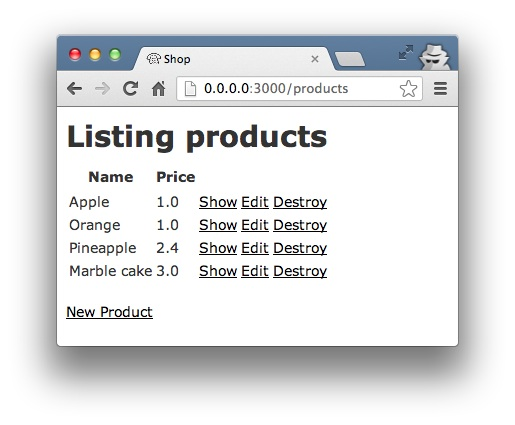
\includegraphics{screenshots/products_index.jpg}
\end{figure}

If you now click the link “New Product”, you will see an input form for a new record:

\begin{figure}[htbp]
\centering
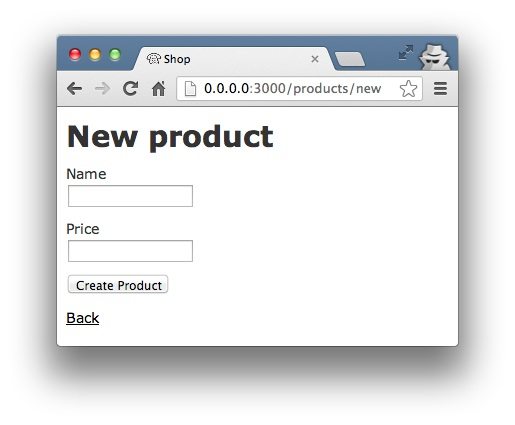
\includegraphics{screenshots/product_new.jpg}
\end{figure}

Use your browser's Back button to go back and click on the “Show” link in the first line. You will then see the following page:

\begin{figure}[htbp]
\centering
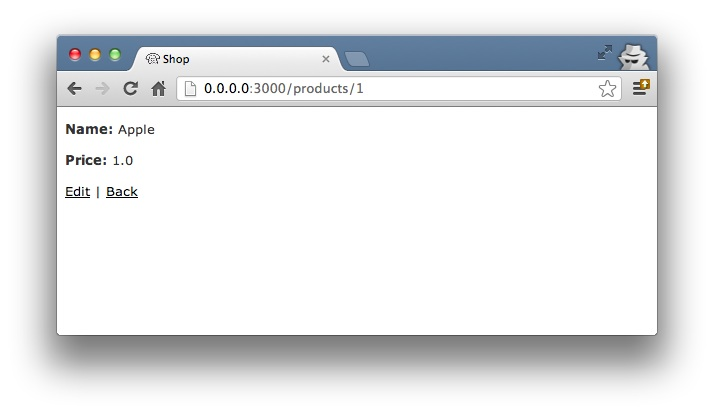
\includegraphics{screenshots/product_show_1.jpg}
\end{figure}

If you now click “Edit”, you will see the editing view for this record:

\begin{figure}[htbp]
\centering
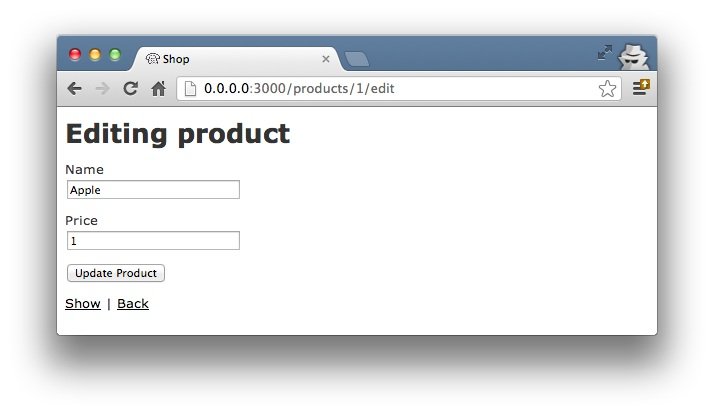
\includegraphics{screenshots/product_edit_1.jpg}
\end{figure}

And if you click “Destroy” on the Index page, you can delete a record after confirming the message that pops up. Isn't that cool?! Within less than 10 minutes, you have written a Web application that allows you to \textbf{c}reate, \textbf{r}ead/\textbf{r}etrieve, \textbf{u}pdate and \textbf{d}elete/\textbf{d}estroy records (CRUD). That is the scaffolding magic. You can save a lot of time.

\chap{Where Are the Views?}\label{where-are-the-views}

You can probably guess, but let's have a look at the directory \texttt{app/views/products} anyway:

\begin{shaded}\begin{verbatim}
$ tree app/views/products/
app/views/products/
├── _form.html.erb
├── edit.html.erb
├── index.html.erb
├── index.json.jbuilder
├── new.html.erb
├── show.html.erb
└── show.json.jbuilder
$
\end{verbatim}\end{shaded}

There are two different file extensions. The \texttt{html.erb} is for HTML requests and the \texttt{json.jbuilder} is for JSON requests.

For \texttt{index}, \texttt{edit}, \texttt{new} and \texttt{show} the corresponding views are located there. As \texttt{new} and \texttt{edit} both require a form for editing the data, this is stored in the partial \texttt{\_form.html.erb} (see \hyperref[partials]{the section called “Partials”}) in accordance with the principle of DRY (\textbf{D}on't \textbf{R}epeat \textbf{Y}ourself) and integrated in \texttt{new.html.erb} and \texttt{edit.html.erb} with a \texttt{\textless{}\%= render 'form'         \%\textgreater{}}.

Let's open the file \texttt{app/views/products/index.html.erb}:

\begin{shaded}\begin{verbatim}
<h1>Listing products</h1>

<table>
  <thead>
    <tr>
      <th>Name</th>
      <th>Price</th>
      <th></th>
      <th></th>
      <th></th>
    </tr>
  </thead>

  <tbody>
    <% @products.each do |product| %>
      <tr>
        <td><%= product.name %></td>
        <td><%= product.price %></td>
        <td><%= link_to 'Show', product %></td>
        <td><%= link_to 'Edit', edit_product_path(product) %></td>
        <td><%= link_to 'Destroy', product, method: :delete, data: { confirm: 'Are you sure?' } %></td>
      </tr>
    <% end %>
  </tbody>
</table>

<br>

<%= link_to 'New Product', new_product_path %>
\end{verbatim}\end{shaded}

You are now an old hand when it comes to ERB, so you'll be able to read and understand the code without any problems. If in doubt, have a quick look at \hyperref[erb-programmieren]{the section called “Programming in an erb File”}.

\chap{link\_to}\label{linkux5fto}

In the views generated by the scaffold generator, you first came across the helper \texttt{link\_to}. This creates \texttt{\textless{}a href         ...\textgreater{}} links. You can of course also enter a link manually via \texttt{\textless{}a href="..."\textgreater{}} in the erb, but for links within a Rails project, \texttt{link\_to} is more practical, because you can use the names of the routes as a target. The code becomes much easier to read. In the above example, there are the following routes:

\begin{shaded}\begin{verbatim}
$ rake routes
      Prefix Verb   URI Pattern                  Controller#Action
    products GET    /products(.:format)          products#index
             POST   /products(.:format)          products#create
 new_product GET    /products/new(.:format)      products#new
edit_product GET    /products/:id/edit(.:format) products#edit
     product GET    /products/:id(.:format)      products#show
             PATCH  /products/:id(.:format)      products#update
             PUT    /products/:id(.:format)      products#update
             DELETE /products/:id(.:format)      products#destroy
$
\end{verbatim}\end{shaded}

The first part of this route is the name of the route. With a new call, this is \texttt{new\_product}. A link to \texttt{new\_product} looks like this in the erb code (you can see it at the end of the file \texttt{app/views/products/index.html.erb}):

\begin{shaded}\begin{verbatim}
<%= link_to 'New Product', new_product_path %>
\end{verbatim}\end{shaded}

In the HTML code of the generated page (\texttt{http://0.0.0.0:3000/products}) you can see the result:

\begin{shaded}\begin{verbatim}
<a href="/products/new">New Product</a>
\end{verbatim}\end{shaded}

With \texttt{link\_to} you can also link to resources within a RESTful resource. Again, you can find examples for this in \texttt{app/views/products/index.html.erb}. In the table, a \texttt{show}, an \texttt{edit} and a \texttt{destroy} link is rendered for each \texttt{product}:

\begin{shaded}\begin{verbatim}
<tbody>
  <% @products.each do |product| %>
    <tr>
      <td><%= product.name %></td>
      <td><%= product.price %></td>
      <td><%= link_to 'Show', product %></td>
      <td><%= link_to 'Edit', edit_product_path(product) %></td>
      <td><%= link_to 'Destroy', product, method: :delete, data: { confirm: 'Are you sure?' } %></td>
    </tr>
  <% end %>
</tbody>
\end{verbatim}\end{shaded}

From the resource and the selected route, Rails automatically determines the required URL and the required HTTP verb (in other words, whether it is a POST, GET, PUT or DELETE). For index and show calls, you need to observe the difference between singular and plural. \texttt{link\_to 'Show', product} links to a single record and \texttt{link\_to 'Show', products\_path} links to the index view.

Whether the name of the route is used with or without the suffix \texttt{\_path} in \texttt{link\_to} depends on whether Rails can “derive” the route from the other specified information. If only one object is specified (in our example, the variable \texttt{product}), then Rails automatically assumes that it is a show route.

Examples:

\begin{longtable}[c]{@{}lp{10cm}@{}}
\caption{~}\\
\toprule\addlinespace
\texttt{link\_to 'Show', Product.first} & Link to the first product.
\\\addlinespace
\texttt{link\_to 'New Product',                 new\_product\_path} & Link to the Web interface where a new product can be created.
\\\addlinespace
\texttt{link\_to 'Edit',                 edit\_product\_path(Product.first)} & Link to the form where the first product can be edited.
\\\addlinespace
\texttt{link\_to 'Destroy', Product.first, method:                 :delete} & Link to deleting the first product.
\\\addlinespace
\bottomrule
\end{longtable}

\section{form\_for}\label{formux5ffor}

In the partial used by \texttt{new} and \texttt{edit}, \texttt{app/views/products/\_form.html.erb}, you will find the following code for the product form:

\begin{shaded}\begin{verbatim}
<%= form_for(@product) do |f| %>
  <% if @product.errors.any? %>
    <div id="error_explanation">
      <h2><%= pluralize(@product.errors.count, "error") %> prohibited this product from being saved:</h2>

      <ul>
      <% @product.errors.full_messages.each do |msg| %>
        <li><%= msg %></li>
      <% end %>
      </ul>
    </div>
  <% end %>

  <div class="field">
    <%= f.label :name %><br>
    <%= f.text_field :name %>
  </div>
  <div class="field">
    <%= f.label :price %><br>
    <%= f.text_field :price %>
  </div>
  <div class="actions">
    <%= f.submit %>
  </div>
<% end %>
\end{verbatim}\end{shaded}

In a block, the helper \texttt{form\_for} takes care of creating the HTML form via which the user can enter the data for the record or edit it. If you delete a complete \texttt{\textless{}div         class="field"\textgreater{}} element here, this can no longer be used for input in the web interface. I am not going to comment on all possible form field variations at this point. The most frequently used ones will appear in examples later on and be explained then (if they are not self-explanatory).

\subsection{Note}\label{note-34}

You can find an overview of all form helpers at \url{http://guides.rubyonrails.org/form_helpers.html}\{.uri\}

When using validations in the model, any validation errors that occur are displayed in the following code at the head of the form:

\begin{shaded}\begin{verbatim}
<% if @product.errors.any? %>
  <div id="error_explanation">
    <h2><%= pluralize(@product.errors.count, "error") %> prohibited this product from being saved:</h2>

    <ul>
    <% @product.errors.full_messages.each do |msg| %>
      <li><%= msg %></li>
    <% end %>
    </ul>
  </div>
<% end %>
\end{verbatim}\end{shaded}

Let's add a small validation to the \texttt{app/models/product.rb} model:

\begin{shaded}\begin{verbatim}
class Product < ActiveRecord::Base
  validates :name,
            presence: true
end
\end{verbatim}\end{shaded}

When ever somebody wants to save a product which doesn't have a name Rails will show this Flash Error:

\begin{figure}[htbp]
\centering
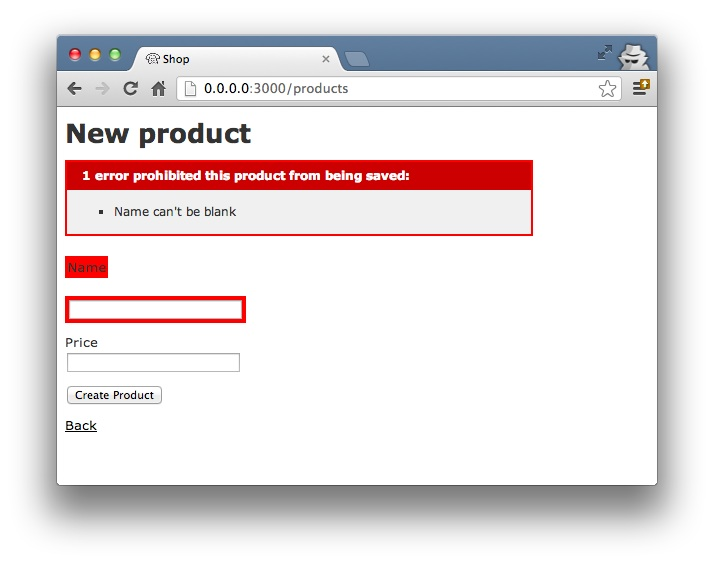
\includegraphics{screenshots/product_error_flash.jpg}
\end{figure}

\section{Access via JSON}\label{access-via-json}

By default, Rails' scaffolding generates not just access via HTML for “human” users, but also a direct interface for machines. The same methods \texttt{index}, \texttt{show}, \texttt{new}, \texttt{create}, \texttt{update} and \texttt{destroy} can be called via this interface, but in a format that is easier to read for machines. As an example, we will demonstrate the \texttt{index} action via which all data can be read in one go. With the same idea, data can be removed (\texttt{destroy}) or edited (\texttt{update}).

JSON (see \href{http://de.wikipedia.org/wiki/JavaScript_Object_Notation}{http://en.wikipedia.org/wiki/Json}) seems to be the new cool kid. So we use JSON.

If you do not require machine-readable access to data, you can skip these examples. But then you should also delete all lines with \texttt{format.json} in the \texttt{respond\_to} blocks of your controllers, to be on the safe side. Otherwise you still have an interface to the data that you may just forget and that constitutes a potential security gap.

\section{JSON as Default}\label{json-as-default}

Right at the beginning of \texttt{app/controllers/products\_controller.rb} you will find the entry for the \texttt{index} action:

\begin{shaded}\begin{verbatim}
## GET /products
## GET /products.json
def index
  @products = Product.all
end
\end{verbatim}\end{shaded}

The code is straightforward. In the instance variable \texttt{@products}, all products are saved. The view \texttt{app/views/products/index.json.jbuilder} contains the following code to render the JSON:

\begin{shaded}\begin{verbatim}
json.array!(@products) do |product|
  json.extract! product, :name, :price
  json.url product_url(product, format: :json)
end
\end{verbatim}\end{shaded}

You can use your browser to fetch the JSON output. Just open \texttt{http://0.0.0.0:3000/products.json} and view the result. I installed a JSON view extension in my Chrome browser to get a nicer format.

\begin{figure}[htbp]
\centering
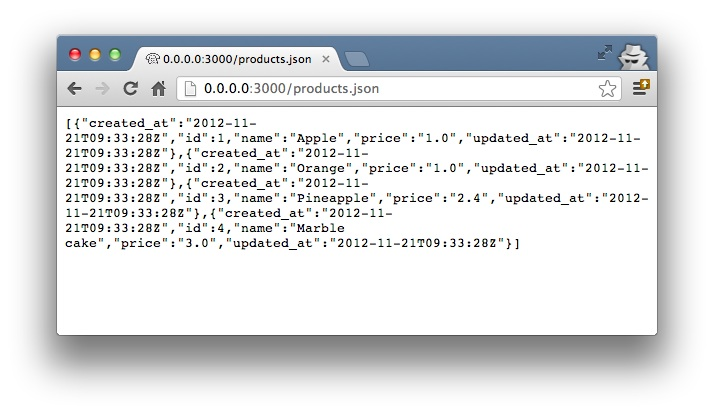
\includegraphics{screenshots/products_index_json.jpg}
\end{figure}

If you do not want the JSON output, you need to delete the \texttt{json.jbuilder} files.

\section{JSON and XML Together}\label{json-and-xml-together}

If you ever need a JSON and XML interface in a Rails application, you just need to specify both variants in the controller in the block \texttt{respond\_to}. Here is an example with the \texttt{app/controllers/products\_controller.rb} in the \texttt{index} action:

\begin{shaded}\begin{verbatim}
## GET /products
## GET /products.json
## GET /products.xml
def index
  @products = product.all

  respond_to do |format|
    format.html # index.html.erb
    format.json { render json: @products }
    format.xml { render xml: @products }
  end
end
\end{verbatim}\end{shaded}

\section{When Should You Use Scaffolding?}\label{when-should-you-use-scaffolding}

You should never use scaffolding just for the sake of it. There are Rails developers who never use scaffolding and always build everything manually. I find scaffolding quite useful for quickly getting into a new project. But it is always just the beginning.

\section{Example for a Minimal Project}\label{example-for-a-minimal-project}

Let's assume we need a web page quickly with which we can list products and represent them individually. But we do not require an editing or deleting function. In that case, a large part of the code created via scaffold would be useless and have to be deleted. Let's try it out as follows:

\begin{shaded}\begin{verbatim}
$ rails new read-only-shop
  [...]
$ cd read-only-shop
$ rails generate scaffold product name 'price:decimal{7,2}'
      invoke  active_record
      create    db/migrate/20130716202340_create_products.rb
      create    app/models/product.rb
      invoke    test_unit
      create      test/models/product_test.rb
      create      test/fixtures/products.yml
      invoke  resource_route
       route    resources :products
      invoke  scaffold_controller
      create    app/controllers/products_controller.rb
      invoke    erb
      create      app/views/products
      create      app/views/products/index.html.erb
      create      app/views/products/edit.html.erb
      create      app/views/products/show.html.erb
      create      app/views/products/new.html.erb
      create      app/views/products/_form.html.erb
      invoke    test_unit
      create      test/controllers/products_controller_test.rb
      invoke    helper
      create      app/helpers/products_helper.rb
      invoke      test_unit
      create        test/helpers/products_helper_test.rb
      invoke    jbuilder
      create      app/views/products/index.json.jbuilder
      create      app/views/products/show.json.jbuilder
      invoke  assets
      invoke    coffee
      create      app/assets/javascripts/products.js.coffee
      invoke    scss
      create      app/assets/stylesheets/products.css.scss
      invoke  scss
   identical    app/assets/stylesheets/scaffolds.css.scss
$ rake db:migrate
  [...]
$
\end{verbatim}\end{shaded}

Now create the \texttt{db/seeds.rb} with some demo products:

\begin{shaded}\begin{verbatim}
Product.create(name: 'Apple', price: 1)
Product.create(name: 'Orange', price: 1)
Product.create(name: 'Pineapple', price: 2.4)
Product.create(name: 'Marble cake', price: 3)
\end{verbatim}\end{shaded}

And populate it with this data:

\begin{shaded}\begin{verbatim}
$ rake db:seed
$
\end{verbatim}\end{shaded}

As we only need \texttt{index} and \texttt{show}, we should delete the not required views:

\begin{shaded}\begin{verbatim}
$ rm app/views/products/_form.html.erb
$ rm app/views/products/new.html.erb
$ rm app/views/products/edit.html.erb
$
\end{verbatim}\end{shaded}

The \texttt{json.jbuilder} views are not needed either:

\begin{shaded}\begin{verbatim}
$ rm app/views/products/*.json.jbuilder
$
\end{verbatim}\end{shaded}

The file \texttt{app/controllers/products\_controller.rb} can be simplified with an editor. It should look like this:

\begin{shaded}\begin{verbatim}
class ProductsController < ApplicationController
  # GET /products
  def index
    @products = Product.all
  end

  # GET /products/1
  def show
    @product = Product.find(params[:id])
  end
end
\end{verbatim}\end{shaded}

We only need the routes for \texttt{index} and \texttt{show}. Please open the file \texttt{config/routes.rb} and edit it as follows:

\begin{shaded}\begin{verbatim}
ReadOnlyShop::Application.routes.draw do
  resources :products, only: [:index, :show]
end
\end{verbatim}\end{shaded}

A \textbf{rake routes} shows us that really only \texttt{index} and \texttt{show} are routed now:

\begin{shaded}\begin{verbatim}
$ rake routes
  Prefix Verb URI Pattern             Controller#Action
products GET /products(.:format)     products#index
 product GET /products/:id(.:format) products#show
$
\end{verbatim}\end{shaded}

If we now start the server \textbf{rails server} and go to the URL \texttt{http://0.0.0.0:3000/products}, we get an error message.

\begin{figure}[htbp]
\centering
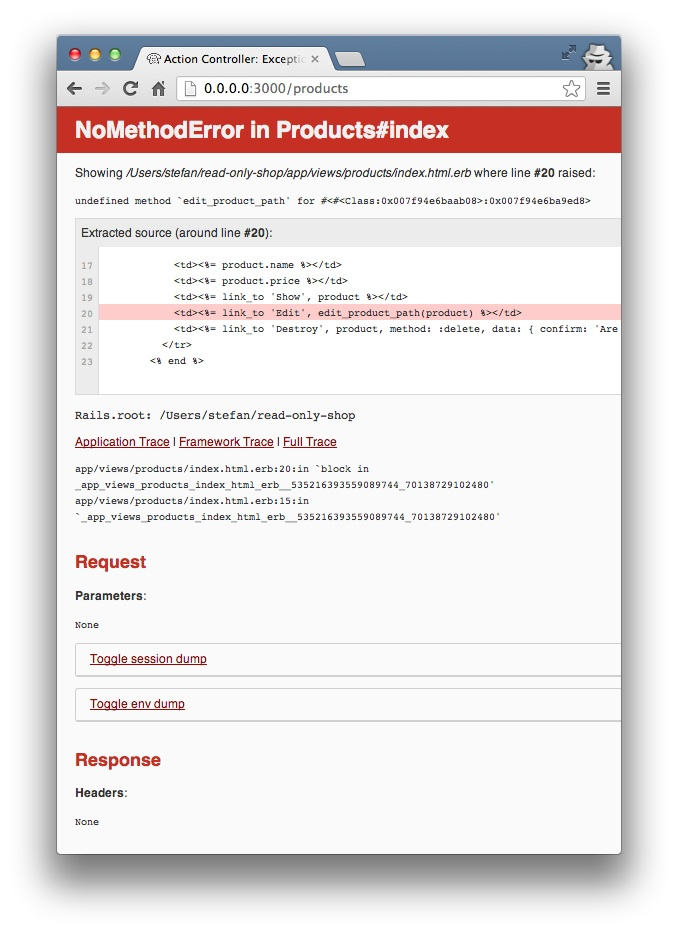
\includegraphics{screenshots/products_routes_error.jpg}
\end{figure}

The same message will be displayed in the log:

\begin{shaded}\begin{verbatim}
$ rails server
=> Booting WEBrick
=> Rails 4.0.0 application starting in development on http://0.0.0.0:3000
=> Run `rails server -h` for more startup options
=> Ctrl-C to shutdown server
[2013-07-16 22:29:42] INFO  WEBrick 1.3.1
[2013-07-16 22:29:42] INFO  ruby 2.0.0 (2013-06-27) [x86_64-darwin12.4.0]
[2013-07-16 22:29:42] INFO  WEBrick::HTTPServer#start: pid=10182 port=3000


Started GET "/products" for 127.0.0.1 at 2013-07-16 22:29:47 +0200
  ActiveRecord::SchemaMigration Load (0.1ms)  SELECT "schema_migrations".* FROM "schema_migrations"
Processing by ProductsController#index as HTML
  Product Load (0.1ms)  SELECT "products".* FROM "products"
  Rendered products/index.html.erb within layouts/application (21.7ms)
Completed 500 Internal Server Error in 61ms

ActionView::Template::Error (undefined method `edit_product_path' for #<#<Class:0x007f94e6baab08>:0x007f94e6ba9ed8>):
    17:         <td><%= product.name %></td>
    18:         <td><%= product.price %></td>
    19:         <td><%= link_to 'Show', product %></td>
    20:         <td><%= link_to 'Edit', edit_product_path(product) %></td>
    21:         <td><%= link_to 'Destroy', product, method: :delete, data: { confirm: 'Are you sure?' } %></td>
    22:       </tr>
    23:     <% end %>
  app/views/products/index.html.erb:20:in `block in _app_views_products_index_html_erb__535216393559089744_70138729102480'
  app/views/products/index.html.erb:15:in `_app_views_products_index_html_erb__535216393559089744_70138729102480'

[...]
\end{verbatim}\end{shaded}

The error message states that we call an undefined method \texttt{edit\_product\_path} in the view \texttt{app/views/products/index.html.erb}. As we only route \texttt{index} and \texttt{show} now, there are no more \texttt{edit}, \texttt{destroy} or \texttt{new} methods any more. So we need to adapt the file \texttt{app/views/products/index.html.erb} in the editor as follows:

\begin{shaded}\begin{verbatim}
<h1>Listing products</h1>

<table>
  <thead>
    <tr>
      <th>Name</th>
      <th>Price</th>
      <th></th>
    </tr>
  </thead>

  <tbody>
    <% @products.each do |product| %>
      <tr>
        <td><%= product.name %></td>
        <td><%= product.price %></td>
        <td><%= link_to 'Show', product %></td>
      </tr>
    <% end %>
  </tbody>
</table>
\end{verbatim}\end{shaded}

And while we are at it, we also edit the \texttt{app/views/products/show.html.erb} accordingly:

\begin{shaded}\begin{verbatim}
<p>
  <strong>Name:</strong>
  <%= @product.name %>
</p>

<p>
  <strong>Price:</strong>
  <%= @product.price %>
</p>

<%= link_to 'Back', products_path %>
\end{verbatim}\end{shaded}

Now our application is finished. Start the Rails server with \textbf{rails server} and open the URL \texttt{http://0.0.0.0:3000/products} in the browser.

\begin{figure}[htbp]
\centering
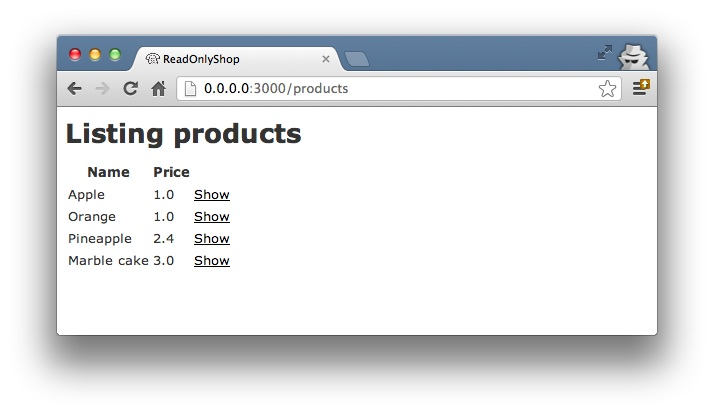
\includegraphics{screenshots/read-only-products-index.jpg}
\end{figure}

\subsection{Note}\label{note-35}

In this example, I am not commenting on the required changes in the tests, as this is not an exercise for test driven development but meant to demonstrate a way of working with scaffolding. TDD developers will quickly be able to adapt the tests.

\section{Conclusion}\label{conclusion}

Have a go and try it out. Try working with scaffolds one time and without them the next. Then you will soon get a feel for whether it fits into your working method or not. I find that scaffolding makes my work much easier for standard applications.

\hyperdef{}{routes}{\chap{Routes}\label{routes}}

\section{Introduction}\label{introduction-2}

In \hyperref[dynamischeux5fwebseiten]{the section called “Creating HTML Dynamically with erb”} and \hyperref[scaffolding]{Chapter~5, \emph{Scaffolding and REST}} we have already come across \emph{routes}. The routes contained in \texttt{config/routes.rb} define what happens in the Rails application when a user of a Rails application fetches a URL. A route can be static and dynamic and pass any dynamic values with variables to the controller. If several routes apply to a URL, the one that is listed at the top of \texttt{config/routes.rb} wins.

\subsection{Tip}\label{tip-14}

If you do not have much time, you can skip this chapter for now and get back to it later if you have any specific questions.

Let's first build a test Rails application so we can experiment:

\begin{shaded}\begin{verbatim}
$ rails new shop
  [...]
$ cd shop
$
\end{verbatim}\end{shaded}

With \textbf{rake routes} we can display the routes of a project. Let's try it straight away in the freshly created project:

\begin{shaded}\begin{verbatim}
$ rake routes
You don't have any routes defined!

Please add some routes in config/routes.rb.

For more information about routes, see the Rails guide: http://guides.rubyonrails.org/routing.html.
$
\end{verbatim}\end{shaded}

That's what I call a good error message. It's a new Rails project, there are no routes yet.

In case of a new Rails project, the file \texttt{config/routes.rb} has many commented out examples. For the rest of this chapter we pretend that these examples are not there and only display the newly entered routes.

\section{HTTP GET Requests for Singular Resources}\label{http-get-requests-for-singular-resources}

As you might know the HTTP protocol uses different so called verbs to access content on the webserver (e.g.~GET to request a page or POST to send a form to the server). First we'll have a look at GET requests.

Create a controller with three pages:

\begin{shaded}\begin{verbatim}
$ rails generate controller Home index ping pong
      create  app/controllers/home_controller.rb
       route  get "home/pong"
       route  get "home/ping"
       route  get "home/index"
       [...]
$
\end{verbatim}\end{shaded}

Now \textbf{rake routes} lists a route for these three pages:

\begin{shaded}\begin{verbatim}
$ rake routes
    Prefix Verb URI Pattern           Controller#Action
home_index GET /home/index(.:format) home#index
 home_ping GET /home/ping(.:format)  home#ping
 home_pong GET /home/pong(.:format)  home#pong
$
\end{verbatim}\end{shaded}

The pages can be accessed at the following URLs after starting the Rails server with \textbf{rails server}:

\begin{itemize}
\itemsep1pt\parskip0pt\parsep0pt
\item
  \texttt{http://0.0.0.0:300/home/index} for \texttt{home\_index GET /home/index(.:format)           home\#index}
\item
  \texttt{http://0.0.0.0:300/home/ping} for \texttt{home\_ping GET /home/ping(.:format)           home\#ping}
\item
  \texttt{http://0.0.0.0:300/home/pong} for \texttt{home\_pong GET /home/pong(.:format)           home\#pong}
\end{itemize}

\begin{figure}[htbp]
\centering
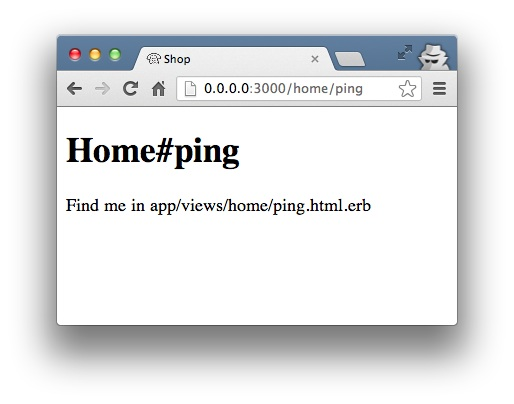
\includegraphics{screenshots/home_ping.jpg}
\end{figure}

With the output \texttt{home\#index}, Rails tells us that the route \texttt{/home/index} goes into the controller \texttt{home} and there to the action/method \texttt{index}. These routes are defined in the file \texttt{config/routes.rb}. \textbf{rails generate controller Home index ping pong} has automatically inserted the following lines there:

\begin{shaded}\begin{verbatim}
  get "home/index"

  get "home/ping"

  get "home/pong"
\end{verbatim}\end{shaded}

\chap{Naming a Route}\label{naming-a-route}

A route should also always have an internal name which doesn't change. In \hyperref[routesux5fget]{the section called “HTTP GET Requests for Singular Resources”} there is the following route:

\begin{shaded}\begin{verbatim}
home_pong GET /home/pong(.:format)  home#pong
\end{verbatim}\end{shaded}

This route has the automatically created name \texttt{home\_pong}. Generally, you should always try to work with the name of the route within a Rails application. So you would point a \texttt{link\_to} to \texttt{home\_pong} and not to \texttt{/home/pong}. This has the big advantage that you can later edit (in the best case, optimize) the routing for visitors externally and do not need to make any changes internally in the application. Of course, you need to enter the old names with \texttt{:as} in that case.

\chap{as}\label{as}

If you want to define the name of a route yourself, you can do so with \texttt{:as}. For example, the line

\begin{shaded}\begin{verbatim}
get "home/pong", as: 'different_name'
\end{verbatim}\end{shaded}

results in the route

\begin{shaded}\begin{verbatim}
different_name GET    /home/pong(.:format)      home#pong
\end{verbatim}\end{shaded}

\chap{to}\label{to}

With to you can define an other destination for a rout. For example, the line

\begin{shaded}\begin{verbatim}
get "home/applepie", to: "home#ping"
\end{verbatim}\end{shaded}

results in the route

\begin{shaded}\begin{verbatim}
home_applepie GET /home/applepie(.:format) home#ping
\end{verbatim}\end{shaded}

\chap{Parameters}\label{parameters}

The routing engine can not just assign fixed routes but also pass parameters which are part of the URL. A typical example would be date specifications (e.g. \url{http://example.com/2010/12/}\{.uri\} for all December postings).

To demonstrate this, let's create a mini blog application:

\begin{shaded}\begin{verbatim}
$ rails new blog
  [...]
$ cd blog
$ rails generate scaffold post subject content published_at:date
  [...]
$ rake db:migrate
  [...]
$
\end{verbatim}\end{shaded}

As example data in the \texttt{db/seeds.rb} we take:

\begin{shaded}\begin{verbatim}
Post.create(subject: 'A test', published_at: '01.10.2011')
Post.create(subject: 'Another test', published_at: '01.10.2011')
Post.create(subject: 'And yet one more test', published_at: '02.10.2011')
Post.create(subject: 'Last test', published_at: '01.11.2011')
Post.create(subject: 'Very final test', published_at: '01.11.2012')
\end{verbatim}\end{shaded}

With \textbf{rake db:seed} we populate the database with this data:

\begin{shaded}\begin{verbatim}
$ rake db:seed
$
\end{verbatim}\end{shaded}

If we now start the Rails server with \textbf{rails server} and go to the page \texttt{http://0.0.0.0:3000/posts} in the browser, we will see this:

\begin{figure}[htbp]
\centering
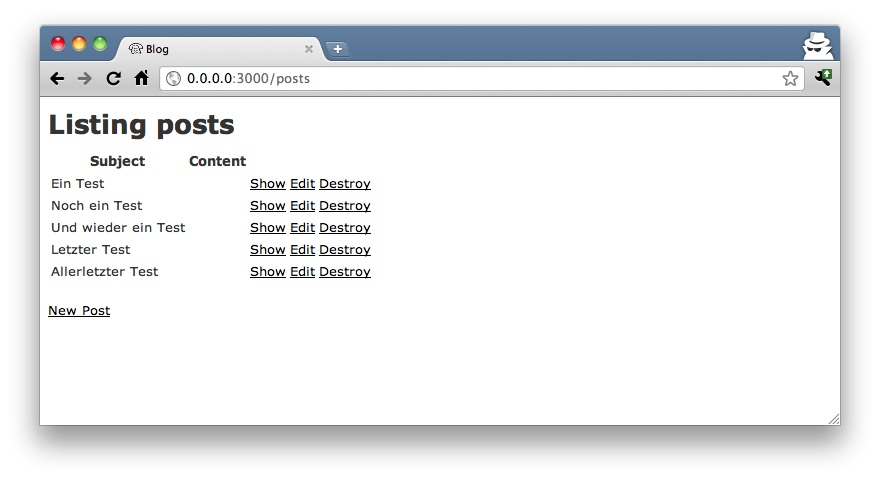
\includegraphics{screenshots/posts_index.jpg}
\end{figure}

For this kind of blog it would of course be very useful if you could render all entries for the year 2010 with the URL \texttt{http://0.0.0.0:3000/2010/} and all entries for October 1st 2010 with \texttt{http://0.0.0.0:3000/2010/10/01}. We can do this by using optional parameters. Please enter the following configuration in the \texttt{config/routes.rb}:

\begin{shaded}\begin{verbatim}
Blog::Application.routes.draw do
  resources :posts

  get ':year(/:month(/:day))', to: 'posts#index'
end
\end{verbatim}\end{shaded}

The round brackets represent optional parameters. In this case, you have to specify the year, but not necessarily the month or day. \textbf{rake routes} shows the new route at the last line:

\begin{shaded}\begin{verbatim}
$ rake routes
   Prefix Verb   URI Pattern                      Controller#Action
    posts GET    /posts(.:format)                 posts#index
          POST   /posts(.:format)                 posts#create
 new_post GET    /posts/new(.:format)             posts#new
edit_post GET    /posts/:id/edit(.:format)        posts#edit
     post GET    /posts/:id(.:format)             posts#show
          PATCH  /posts/:id(.:format)             posts#update
          PUT    /posts/:id(.:format)             posts#update
          DELETE /posts/:id(.:format)             posts#destroy
          GET    /:year(/:month(/:day))(.:format) posts#index
$
\end{verbatim}\end{shaded}

If we do not change anything else, we still get the same result when calling \texttt{http://0.0.0.0:3000/2011/} and \texttt{http://0.0.0.0:3000/2011/10/01} as we did with \texttt{http://0.0.0.0:3000/posts}. But have a look at the output of rails server for the request \texttt{http://0.0.0.0:3000/2011}

\begin{shaded}\begin{verbatim}
Started GET "/2011" for 127.0.0.1 at 2013-07-17 11:08:58 +0200
  ActiveRecord::SchemaMigration Load (0.1ms)  SELECT "schema_migrations".* FROM "schema_migrations"
Processing by PostsController#index as HTML
  Parameters: {"year"=>"2011"}
  Post Load (0.1ms)  SELECT "posts".* FROM "posts"
  Rendered posts/index.html.erb within layouts/application (21.3ms)
Completed 200 OK in 96ms (Views: 76.3ms | ActiveRecord: 0.5ms)
\end{verbatim}\end{shaded}

The route has been recognised and an \texttt{"year" =\textgreater{}       "2011"} has been assigned to the hash \texttt{params} (written misleadingly as \texttt{Parameters} in the output). Going to the URL \texttt{http://0.0.0.0:3000/2010/12/24} results in the following output, as expected:

\begin{shaded}\begin{verbatim}
Started GET "/2010/12/24" for 127.0.0.1 at 2013-07-17 11:11:21 +0200
Processing by PostsController#index as HTML
  Parameters: {"year"=>"2010", "month"=>"12", "day"=>"24"}
  Post Load (0.2ms)  SELECT "posts".* FROM "posts"
  Rendered posts/index.html.erb within layouts/application (3.4ms)
Completed 200 OK in 9ms (Views: 8.1ms | ActiveRecord: 0.2ms)
\end{verbatim}\end{shaded}

In case of the URL \texttt{http://0.0.0.0:3000/2010/12/24}, the following values have been saved in the hash \texttt{params}: \texttt{"year"=\textgreater{}"2010", "month"=\textgreater{}"12",       "day"=\textgreater{}"24".}

In the controller, we can access \texttt{params{[}{]}} to access the values defined in the URL. We simply need to adapt the \texttt{index} method in \texttt{app/controllers/posts\_controller.rb} to output the \texttt{posts} entered for the corresponding date, month or year:

\begin{shaded}\begin{verbatim}
## GET /posts
## GET /posts.json
def index
  # Check if the URL requests a date.
  if Date.valid_date? params[:year].to_i, params[:month].to_i, params[:day].to_i
    start_date = Date.parse("#{params[:day]}.#{params[:month]}.#{params[:year]}")
    end_date = start_date

  # Check if the URL requests a month
  elsif Date.valid_date? params[:year].to_i, params[:month].to_i, 1
    start_date = Date.parse("1.#{params[:month]}.#{params[:year]}")
    end_date = start_date.end_of_month

  # Check if the URL requests a year
  elsif params[:year] && Date.valid_date?(params[:year].to_i, 1, 1)
    start_date = Date.parse("1.1.#{params[:year]}")
    end_date = start_date.end_of_year
  end

  if start_date && end_date
    @posts = Post.where(published_at: start_date..end_date)
  else
    @posts = Post.all
  end
end
\end{verbatim}\end{shaded}

If we now go to \texttt{http://0.0.0.0:3000/2011/10/01} , we can see all \texttt{posts} of October 1st 2011.

\begin{figure}[htbp]
\centering
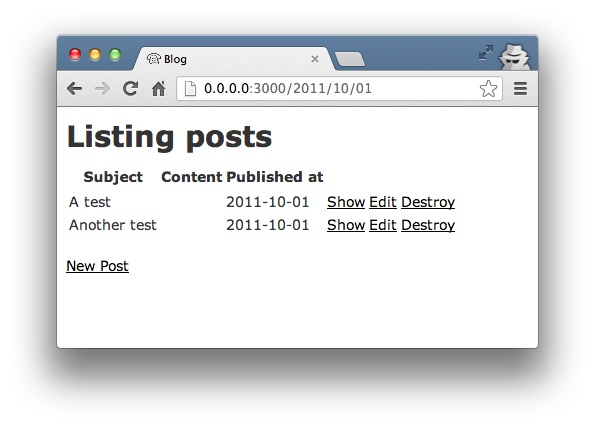
\includegraphics{screenshots/posts_2011_10_01.jpg}
\end{figure}

\chap{Constraints}\label{constraints}

In \hyperref[routesux5fmatchux5fparameter]{the section called “Parameters”} I showed you how you can read out parameters from the URL and pass them to the controller. Unfortunately, the entry defined there in the \texttt{config/routes.rb}

\begin{shaded}\begin{verbatim}
get ':year(/:month(/:day))', to: 'posts#index'
\end{verbatim}\end{shaded}

has one important disadvantage: it does not verify the individual elements. For example, the URL \texttt{http://0.0.0.0:3000/just/an/example} will be matched just the same and then of course results in an error:

\begin{figure}[htbp]
\centering
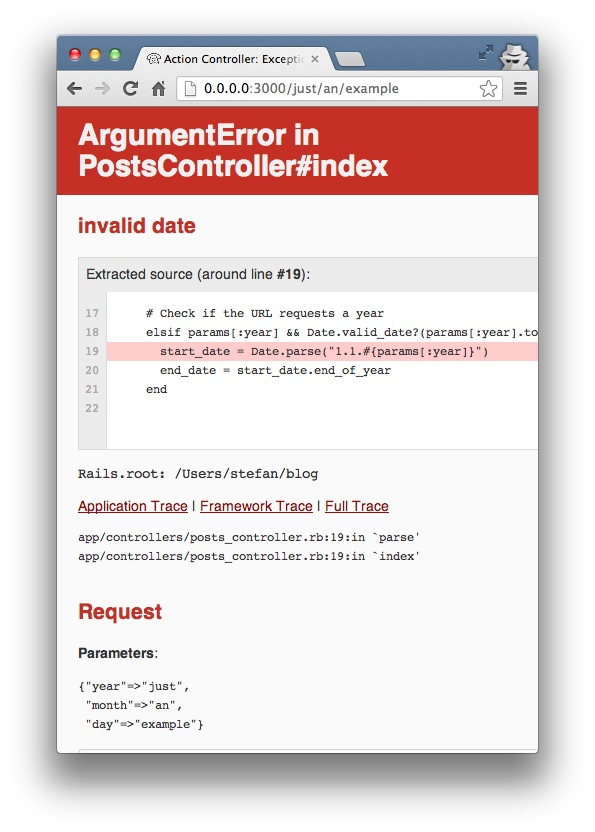
\includegraphics{screenshots/ein_beispiel_dafuer_fehler.jpg}
\end{figure}

In the log output in\texttt{log/development.log} we can see the following entry:

\begin{shaded}\begin{verbatim}
Started GET "/just/an/example" for 127.0.0.1 at 2013-07-17 12:04:01 +0200
Processing by PostsController#index as HTML
  Parameters: {"year"=>"just", "month"=>"an", "day"=>"example"}
Completed 500 Internal Server Error in 2ms

ArgumentError (invalid date):
  app/controllers/posts_controller.rb:19:in `parse'
  app/controllers/posts_controller.rb:19:in `index'
\end{verbatim}\end{shaded}

Obviously, \texttt{Date.parse( "example.an.just")} cannot work. A date is made up of numbers, not letters.

Constraints can define the content of the URL more precisely via regular expressions. In the case of our blog, the \texttt{config/routes.rb} with contraints would look like this:

\begin{shaded}\begin{verbatim}
Blog::Application.routes.draw do
  resources :posts

  get ':year(/:month(/:day))', to: 'posts#index', constraints: { year: /\d{4}/, month: /\d{2}/, day: /\d{2}/ }
end
\end{verbatim}\end{shaded}

\subsection{Warning}\label{warning-10}

Please note that you cannot use regex anchors such as “\^{}” in regular expressions in a constraint.

If we go to the URL again with this configuration, Rails gives us an error message “No route matches”:

\begin{figure}[htbp]
\centering
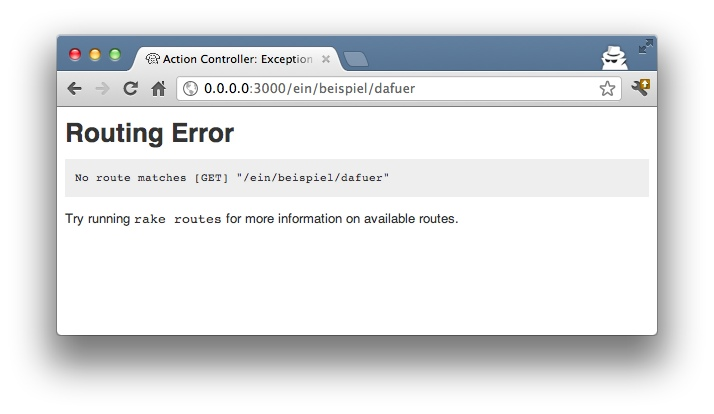
\includegraphics{screenshots/ein_beispiel_dafuer_no_route_matches.jpg}
\end{figure}

\section{Redirects}\label{redirects-1}

Our current application answers request in the format YYYY/MM/DD (4 digits for the year, 2 digits for the month and 2 digits for the day). That is ok for machines but maybe a human would request a single digit month (like January) and a single digit day without adding the extra 0 to make it two digits. We can fix that with a couple of redirect rules which catch these URLs and redirect them to the correct ones.

\begin{shaded}\begin{verbatim}
Blog::Application.routes.draw do
  resources :posts

  get ':year/:month/:day', to: redirect("/%{year}/0%{month}/0%{day}"), constraints: { year: /\d{4}/, month: /\d{1}/, day: /\d{1}/ }
  get ':year/:month/:day', to: redirect("/%{year}/0%{month}/%{day}"), constraints: { year: /\d{4}/, month: /\d{1}/, day: /\d{2}/ }
  get ':year/:month/:day', to: redirect("/%{year}/%{month}/0%{day}"), constraints: { year: /\d{4}/, month: /\d{2}/, day: /\d{1}/ }
  get ':year/:month', to: redirect("/%{year}/0%{month}"), constraints: { year: /\d{4}/, month: /\d{1}/ }

  get ':year(/:month(/:day))', to: 'posts#index', constraints: { year: /\d{4}/, month: /\d{2}/, day: /\d{2}/ }
end
\end{verbatim}\end{shaded}

With this set of redirect rules, we can ensure that a user of the page can also enter single-digit days and months and still ends up in the right place, or is redirected to the correct format.

\subsection{Note}\label{note-36}

Redirects in the \texttt{config/routes.rb} are by default http redirects with the code 301 (“Moved Permanently”). So even search engines will profit from this.

\section{root :to =\textgreater{} `welcome\#index'}\label{root-to-welcomeindex}

In the default \texttt{config/routes.rb} file you will find the following comment quite a long way down:

\begin{shaded}\begin{verbatim}
## You can have the root of your site routed with "root"
## root 'welcome#index'
\end{verbatim}\end{shaded}

If you comment out the last line there, you can define your \texttt{http://0.0.0.0:3000/} with it. Let's put it on \texttt{home\#index}:

\begin{shaded}\begin{verbatim}
Shop::Application.routes.draw do
  get "home/index"

  get "home/ping"

  get "home/pong"

  root 'home#index'
end
\end{verbatim}\end{shaded}

Our new routes:

\begin{shaded}\begin{verbatim}
$ rake routes
    Prefix Verb URI Pattern           Controller#Action
home_index GET /home/index(.:format) home#index
 home_ping GET /home/ping(.:format)  home#ping
 home_pong GET /home/pong(.:format)  home#pong
      root GET /                     home#index
$
\end{verbatim}\end{shaded}

If we go to the root URL \texttt{http://0.0.0.0:3000} we now see \texttt{home\#index}.

\begin{figure}[htbp]
\centering
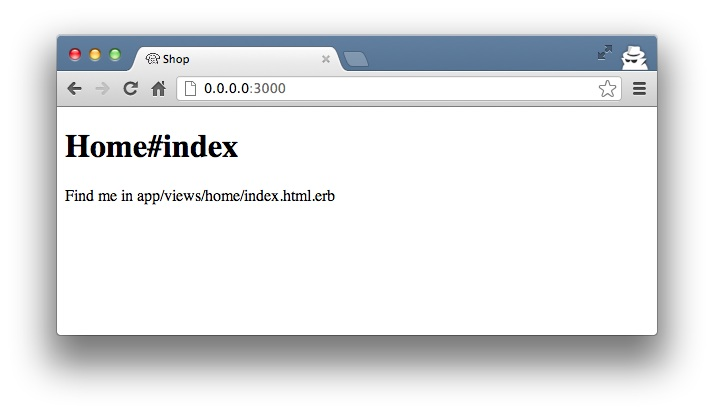
\includegraphics{screenshots/routes_root_url.jpg}
\end{figure}

\section{resources}\label{resources}

\texttt{resources} provides routes for a RESTful resource. Let's try it with the mini blog application:

\begin{shaded}\begin{verbatim}
$ rails new blog
  [...]
$ cd blog
$ rails generate scaffold post subject content published_at:date
  [...]
$ rake db:migrate
  [...]
$
\end{verbatim}\end{shaded}

The scaffold generator automatically creates a \texttt{resources} route in the \texttt{config/routes.rb}:

\begin{shaded}\begin{verbatim}
Blog::Application.routes.draw do
  resources :posts
end
\end{verbatim}\end{shaded}

\subsection{Note}\label{note-37}

New routes are always added at the beginning of \texttt{config/routes.rb} by rails generate scripts.

The resulting routes:

\begin{shaded}\begin{verbatim}
$ rake routes
   Prefix Verb   URI Pattern               Controller#Action
    posts GET    /posts(.:format)          posts#index
          POST   /posts(.:format)          posts#create
 new_post GET    /posts/new(.:format)      posts#new
edit_post GET    /posts/:id/edit(.:format) posts#edit
     post GET    /posts/:id(.:format)      posts#show
          PATCH  /posts/:id(.:format)      posts#update
          PUT    /posts/:id(.:format)      posts#update
          DELETE /posts/:id(.:format)      posts#destroy
$
\end{verbatim}\end{shaded}

You have already encountered these RESTful routes in \hyperref[scaffolding]{Chapter~5, \emph{Scaffolding and REST}}. They are required for displaying and editing records.

\chap{Selecting Specific Routes with only: or except:}\label{selecting-specific-routes-with-only-or-except}

If you only want to use specific routes from the finished set of RESTful routes, you can limit them with \texttt{:only} or \texttt{:except}.

The following \texttt{conf/routes.rb} defines only the routes for \texttt{index} and \texttt{show}:

\begin{shaded}\begin{verbatim}
Blog::Application.routes.draw do
  resources :posts, only: [:index, :show]
end
\end{verbatim}\end{shaded}

With \textbf{rake routes} we can check the result:

\begin{shaded}\begin{verbatim}
$ rake routes
Prefix Verb URI Pattern          Controller#Action
posts GET /posts(.:format)     posts#index
 post GET /posts/:id(.:format) posts#show
$
\end{verbatim}\end{shaded}

\texttt{except} works exactly the other way round:

\begin{shaded}\begin{verbatim}
Blog::Application.routes.draw do
  resources :posts, except: [:index, :show]
end
\end{verbatim}\end{shaded}

Now all routes except for \texttt{index} and \texttt{show} are possible:

\begin{shaded}\begin{verbatim}
$ rake routes
   Prefix Verb   URI Pattern               Controller#Action
    posts POST   /posts(.:format)          posts#create
 new_post GET    /posts/new(.:format)      posts#new
edit_post GET    /posts/:id/edit(.:format) posts#edit
     post PATCH  /posts/:id(.:format)      posts#update
          PUT    /posts/:id(.:format)      posts#update
          DELETE /posts/:id(.:format)      posts#destroy
$
\end{verbatim}\end{shaded}

\subsection{Warning}\label{warning-11}

When using \texttt{only} and \texttt{except}, please make sure you also adapt the views generated by the scaffold generator. For example, there is a link on the index page to the new view with \texttt{\textless{}\%= link\_to 'New Post', new\_post\_path \%\textgreater{}} but this view no longer exists in the above only example.

\section{Nested Resources}\label{nested-resources}

Nested resources refer to routes of resources that work with a association (see \hyperref[activerecordux5fhasux5fmany]{the section called “has\_many -- 1:n Association”}). These can be addressed precisely via routes. Let's create a second resource, \texttt{comment}:

\begin{shaded}\begin{verbatim}
$ rails generate scaffold comment post_id:integer content
  [...]
$ rake db:migrate
  [...]
$
\end{verbatim}\end{shaded}

Now we associate the two resources. In the file \texttt{app/models/post.rb}, we add a \texttt{has\_many}:

\begin{shaded}\begin{verbatim}
class Post < ActiveRecord::Base
  has_many :comments
end
\end{verbatim}\end{shaded}

And in the file \texttt{app/models/comment.rb}, its counterpart \texttt{belongs\_to}:

\begin{shaded}\begin{verbatim}
class Comment < ActiveRecord::Base
  belongs_to :post
end
\end{verbatim}\end{shaded}

The routes generated by the scaffold generator look like this:

\begin{shaded}\begin{verbatim}
$ rake routes
      Prefix Verb   URI Pattern                  Controller#Action
    comments GET    /comments(.:format)          comments#index
             POST   /comments(.:format)          comments#create
 new_comment GET    /comments/new(.:format)      comments#new
edit_comment GET    /comments/:id/edit(.:format) comments#edit
     comment GET    /comments/:id(.:format)      comments#show
             PATCH  /comments/:id(.:format)      comments#update
             PUT    /comments/:id(.:format)      comments#update
             DELETE /comments/:id(.:format)      comments#destroy
       posts GET    /posts(.:format)             posts#index
             POST   /posts(.:format)             posts#create
    new_post GET    /posts/new(.:format)         posts#new
   edit_post GET    /posts/:id/edit(.:format)    posts#edit
        post GET    /posts/:id(.:format)         posts#show
             PATCH  /posts/:id(.:format)         posts#update
             PUT    /posts/:id(.:format)         posts#update
             DELETE /posts/:id(.:format)         posts#destroy
$
\end{verbatim}\end{shaded}

So we can get the first post with \texttt{/posts/1} and all the comments with \texttt{/comments}. By using nesting, we can get all comments with the ID 1 via \texttt{/posts/1/}comments. We need to change the \texttt{config/routes.rb}:

\begin{shaded}\begin{verbatim}
Blog::Application.routes.draw do
  resources :posts do
    resources :comments
  end
end
\end{verbatim}\end{shaded}

This gives us the desired routes:

\begin{shaded}\begin{verbatim}
$ rake routes
           Prefix Verb   URI Pattern                                 Controller#Action
    post_comments GET    /posts/:post_id/comments(.:format)          comments#index
                  POST   /posts/:post_id/comments(.:format)          comments#create
 new_post_comment GET    /posts/:post_id/comments/new(.:format)      comments#new
edit_post_comment GET    /posts/:post_id/comments/:id/edit(.:format) comments#edit
     post_comment GET    /posts/:post_id/comments/:id(.:format)      comments#show
                  PATCH  /posts/:post_id/comments/:id(.:format)      comments#update
                  PUT    /posts/:post_id/comments/:id(.:format)      comments#update
                  DELETE /posts/:post_id/comments/:id(.:format)      comments#destroy
            posts GET    /posts(.:format)                            posts#index
                  POST   /posts(.:format)                            posts#create
         new_post GET    /posts/new(.:format)                        posts#new
        edit_post GET    /posts/:id/edit(.:format)                   posts#edit
             post GET    /posts/:id(.:format)                        posts#show
                  PATCH  /posts/:id(.:format)                        posts#update
                  PUT    /posts/:id(.:format)                        posts#update
                  DELETE /posts/:id(.:format)                        posts#destroy
$
\end{verbatim}\end{shaded}

But we still need to make some changes in the file \texttt{app/controllers/comments\_controller.rb}. This ensures that only the \texttt{Comments} of the specified \texttt{Post} can be displayed or changed:

\begin{shaded}\begin{verbatim}
class CommentsController < ApplicationController
  before_action :set_post
  before_action :set_comment, only: [:show, :edit, :update, :destroy]

  # GET /comments
  # GET /comments.json
  def index
    @comments = Comment.all
  end

  # GET /comments/1
  # GET /comments/1.json
  def show
  end

  # GET /comments/new
  def new
    @comment = @post.comments.build
  end

  # GET /comments/1/edit
  def edit
  end

  # POST /comments
  # POST /comments.json
  def create
    @comment = @post.comments.build(comment_params)

    respond_to do |format|
      if @comment.save
        format.html { redirect_to @comment, notice: 'Comment was successfully created.' }
        format.json { render action: 'show', status: :created, location: @comment }
      else
        format.html { render action: 'new' }
        format.json { render json: @comment.errors, status: :unprocessable_entity }
      end
    end
  end

  # PATCH/PUT /comments/1
  # PATCH/PUT /comments/1.json
  def update
    respond_to do |format|
      if @comment.update(comment_params)
        format.html { redirect_to @comment, notice: 'Comment was successfully updated.' }
        format.json { head :no_content }
      else
        format.html { render action: 'edit' }
        format.json { render json: @comment.errors, status: :unprocessable_entity }
      end
    end
  end

  # DELETE /comments/1
  # DELETE /comments/1.json
  def destroy
    @comment.destroy
    respond_to do |format|
      format.html { redirect_to comments_url }
      format.json { head :no_content }
    end
  end

  private
    def set_post
      @post = Post.find(params[:post_id])
    end

    # Use callbacks to share common setup or constraints between actions.
    def set_comment
      @comment = @post.comments.find(params[:id])
    end

    # Never trust parameters from the scary internet, only allow the white list through.
    def comment_params
      params.require(:comment).permit(:post_id, :content)
    end
end
\end{verbatim}\end{shaded}

Unfortunately, this is only half the story, because the views still link to the old routes. So we need to adapt each view in accordance with the nested route.

\texttt{app/views/comments/\_form.html.erb}

Please note that you need to change the \texttt{form\_for} call to \texttt{form\_for({[}@post, @comment{]})}.

\begin{shaded}\begin{verbatim}
<%= form_for([@post, @comment]) do |f| %>
  <% if @comment.errors.any? %>
    <div id="error_explanation">
      <h2><%= pluralize(@comment.errors.count, "error") %> prohibited this comment from being saved:</h2>

      <ul>
      <% @comment.errors.full_messages.each do |msg| %>
        <li><%= msg %></li>
      <% end %>
      </ul>
    </div>
  <% end %>

  <div class="field">
    <%= f.label :content %><br />
    <%= f.text_field :content %>
  </div>
  <div class="actions">
    <%= f.submit %>
  </div>
<% end %>
\end{verbatim}\end{shaded}

\texttt{app/views/comments/edit.html.erb}

\begin{shaded}\begin{verbatim}
<h1>Editing comment</h1>

<%= render 'form' %>

<%= link_to 'Show', [@post, @comment] %> |
<%= link_to 'Back', post_comments_path(@post) %>
\end{verbatim}\end{shaded}

\texttt{app/views/comments/index.html.erb}

\begin{shaded}\begin{verbatim}
<h1>Listing comments</h1>

<table>
  <thead>
    <tr>
      <th>Post</th>
      <th>Content</th>
      <th></th>
      <th></th>
      <th></th>
    </tr>
  </thead>

  <tbody>
    <% @comments.each do |comment| %>
      <tr>
        <td><%= comment.post_id %></td>
        <td><%= comment.content %></td>
        <td><%= link_to 'Show', [@post, comment] %></td>
        <td><%= link_to 'Edit', edit_post_comment_path(@post, comment) %></td>
        <td><%= link_to 'Destroy', [@post, comment], method: :delete, data: { confirm: 'Are you sure?' } %></td>
      </tr>
    <% end %>
  </tbody>
</table>

<br>

<%= link_to 'New Comment', new_post_comment_path(@post) %>
\end{verbatim}\end{shaded}

\texttt{app/views/comments/new.html.erb}

\begin{shaded}\begin{verbatim}
<h1>New comment</h1>

<%= render 'form' %>

<%= link_to 'Back', post_comments_path(@post) %>
\end{verbatim}\end{shaded}

\texttt{app/views/comments/show.html.erb}

\begin{shaded}\begin{verbatim}
<p id="notice"><%= notice %></p>

<p>
  <b>Post:</b>
  <%= @comment.post_id %>
</p>

<p>
  <b>Content:</b>
  <%= @comment.content %>
</p>


<%= link_to 'Edit', edit_post_comment_path(@post, @comment) %> |
<%= link_to 'Back', post_comments_path(@post) %>
\end{verbatim}\end{shaded}

Please go ahead and have a go at experimenting with the URLs listed under rake routes. You can now generate a new post with \texttt{/posts/new} and a new comment for this post with \texttt{/posts/:post\_id/comments/new}.

If you want to see all comments of the first post you can access that with the URL \texttt{http://0.0.0.0:3000/posts/1/comments}. It would look like this:

\begin{figure}[htbp]
\centering
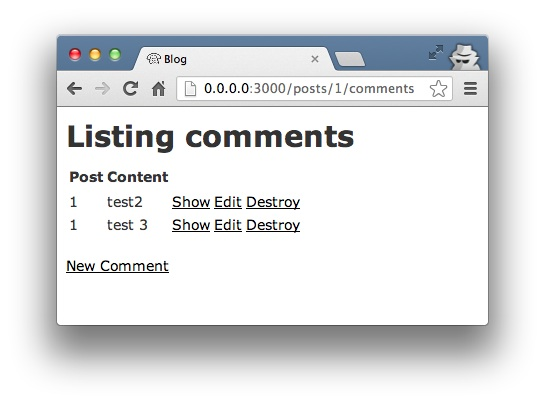
\includegraphics{screenshots/posts_1_comments.jpg}
\end{figure}

\chap{Shallow Nesting}\label{shallow-nesting}

Sometimes it is a better option to use shallow nesting. For our example the \texttt{config/routes.rb} would contain the following routes:

\begin{shaded}\begin{verbatim}
Blog::Application.routes.draw do
  resources :posts do
    resources :comments, only: [:index, :new, :create]
  end

  resources :comments, except: [:index, :new, :create]
end
\end{verbatim}\end{shaded}

That would lead to a less messy \textbf{rake routes} output:

\begin{shaded}\begin{verbatim}
$ rake routes
          Prefix Verb   URI Pattern                            Controller#Action
   post_comments GET    /posts/:post_id/comments(.:format)     comments#index
                 POST   /posts/:post_id/comments(.:format)     comments#create
new_post_comment GET    /posts/:post_id/comments/new(.:format) comments#new
           posts GET    /posts(.:format)                       posts#index
                 POST   /posts(.:format)                       posts#create
        new_post GET    /posts/new(.:format)                   posts#new
       edit_post GET    /posts/:id/edit(.:format)              posts#edit
            post GET    /posts/:id(.:format)                   posts#show
                 PATCH  /posts/:id(.:format)                   posts#update
                 PUT    /posts/:id(.:format)                   posts#update
                 DELETE /posts/:id(.:format)                   posts#destroy
    edit_comment GET    /comments/:id/edit(.:format)           comments#edit
         comment GET    /comments/:id(.:format)                comments#show
                 PATCH  /comments/:id(.:format)                comments#update
                 PUT    /comments/:id(.:format)                comments#update
                 DELETE /comments/:id(.:format)                comments#destroy
$
\end{verbatim}\end{shaded}

Shallow nesting trys to combine the best of two worlds. And because it is often used there is a shortcut. You can use the following \texttt{config/routes.rb} to achieve it:

\begin{shaded}\begin{verbatim}
Blog::Application.routes.draw do
  resources :posts do
    resources :comments, shallow: true
  end
end
\end{verbatim}\end{shaded}

\section{Comments on Nested Resources}\label{comments-on-nested-resources}

Generally, you should never nest more deeply than one level and nested resources should feel natural. After a while, you will get a feel for it. In my opinion, the most important point about RESTful routes is that they should feel logical. If you phone a fellow Rails programmer and say “I've got a resource post and a resource comment here”, then both parties should immediately be clear on how you address these resources via REST and how you can nest them.

\section{Further Information on Routes}\label{further-information-on-routes}

The topic routes is far more complex than we can address here. For example, you can also involve other HTTP methods/verbs. The official routing documentation \url{http://guides.rubyonrails.org/routing.html}\{.uri\} will give you a lot of information an examples for these features and edge cases.

\chap{Tests}\label{tests}

\section{Introduction}\label{introduction-3}

I have been programming for 30 years and most of the time I have managed quite well without test-driven development (TDD). I am not going to be mad at IT dinosaurs if they decide to just skip this chapter. You can create Rails applications without tests and are not likely to get any bad karma as a result (at least, I hope not - but you can never be entirely sure with the whole karma thing).

But if you should decide to go for TDD, then I can promise you that it is an enlightenment. The basic idea of TDD is that you write a test for each programming function to check this function. In the pure TDD teaching, this test is written before the actual programming. Yes, you will have a lot more to do initially. But later, you can run all the tests and see that the application works exactly as you wanted it to. The read advantage only becomes apparent after a few weeks or months, when you look at the project again and write an extension or new variation. Then you can safely change the code and check it still works properly by running the tests. This avoids a situation where you find yourself saying “oops, that went a bit wrong, I just didn't think of this particular problem”.

Often, the advantage of TDD already becomes evident when writing a program. Tests can reveal many careless mistakes that you would otherwise only have stumbled across much later on.

This chapter is a brief overview of the topic test-driven development with Rails. If you have tasted blood and want to find out more, you can dive into the official Rails documentation at \url{http://guides.rubyonrails.org/testing.html}\{.uri\}.

\subsection{Note}\label{note-38}

TDD is just like driving a car. The only way to learn it is by doing it.

\section{Example for a User in a Web Shop}\label{example-for-a-user-in-a-web-shop}

Let's start with a user scaffold in an imaginary web shop:

\begin{shaded}\begin{verbatim}
$ rails new webshop
  [...]
$ cd webshop
$ rails generate scaffold user login_name first_name last_name birthday:date
      [...]
      invoke    test_unit
      create      test/models/user_test.rb
      create      test/fixtures/users.yml
      [...]
      invoke    test_unit
      create      test/controllers/users_controller_test.rb
      invoke    helper
      [...]
      invoke      test_unit
      create        test/helpers/users_helper_test.rb
      [...]
$ rake db:migrate
      [...]
$
\end{verbatim}\end{shaded}

You already know all about scaffolds (if not, please go and read \hyperref[scaffolding]{Chapter~5, \emph{Scaffolding and REST}} first) so you know what the application we have just created does. The scaffold created a few tests (they are easy to recognise because the word \texttt{test} is in the file name).

The complete test suite of a Rails project is processed with the command \textbf{rake test}. Let's have a go and see what a test produces at this stage of development:

\begin{shaded}\begin{verbatim}
$ rake test
Run options: --seed 23117

# Running tests:

.......

Finished tests in 0.696922s, 10.0442 tests/s, 18.6535 assertions/s.

7 tests, 13 assertions, 0 failures, 0 errors, 0 skips
$
\end{verbatim}\end{shaded}

The output “\texttt{7 tests, 13 assertions, 0 failures, 0 errors, 0     skips}” looks good. By default, a test will run correctly in a standard scaffold.

Let's now edit the \texttt{app/models/user.rb} and insert a few validations (if these are not entirely clear to you, please read \hyperref[activerecordux5fvalidation]{the section called “Validation”}):

\begin{shaded}\begin{verbatim}
class User < ActiveRecord::Base
  validates :login_name,
            presence: true,
            length: { minimum: 10 }

  validates :last_name,
            presence: true
end
\end{verbatim}\end{shaded}

Then we execute \textbf{rake test} again:

\begin{shaded}\begin{verbatim}
$ rake test
Run options: --seed 51265

# Running tests:

F.....F

Finished tests in 0.178619s, 39.1896 tests/s, 55.9851 assertions/s.

  1) Failure:
UsersControllerTest#test_should_create_user [/Users/stefan/webshop/test/controllers/users_controller_test.rb:20]:
"User.count" didn't change by 1.
Expected: 3
  Actual: 2

  2) Failure:
UsersControllerTest#test_should_update_user [/Users/stefan/webshop/test/controllers/users_controller_test.rb:39]:
Expected response to be a <redirect>, but was <200>

7 tests, 10 assertions, 2 failures, 0 errors, 0 skips
$
\end{verbatim}\end{shaded}

Boom! This time we have “\texttt{2 failures}”. The error happens in the “\texttt{should create user}” and the “\texttt{should update user}”. The explanation for this is in our validation. The example data created by the scaffold generator went through in the first \textbf{rake test} (without validation). The errors only occurred the second time (with validation).

This example data is created as \emph{fixtures} in YAML format in the directory \texttt{test/fixtures/}. Let's have a look at the example data for \texttt{User} in the file \texttt{test/fixtures/users.yml}:

\begin{shaded}\begin{verbatim}
one:
  login_name: MyString
  first_name: MyString
  last_name: MyString
  birthday: 2013-07-17

two:
  login_name: MyString
  first_name: MyString
  last_name: MyString
  birthday: 2013-07-17
\end{verbatim}\end{shaded}

There are two example records there that do not fulfil the requirements of our validation. The \texttt{login\_name} should have a length of at least 10. Let's change the \texttt{login\_name} in \texttt{test/fixtures/users.yml} accordingly:

\begin{shaded}\begin{verbatim}
one:
  login_name: MyString12
  first_name: MyString
  last_name: MyString
  birthday: 2013-07-17

two:
  login_name: MyString12
  first_name: MyString
  last_name: MyString
  birthday: 2013-07-17
\end{verbatim}\end{shaded}

Now, a \textbf{rake test} completes without any errors again:

\begin{shaded}\begin{verbatim}
$ rake test
Run options: --seed 2058

## Running tests:

.......

Finished tests in 0.150927s, 46.3800 tests/s, 86.1344 assertions/s.

7 tests, 13 assertions, 0 failures, 0 errors, 0 skips
$
\end{verbatim}\end{shaded}

We now know that valid data has to be contained in the \texttt{test/fixtures/users.yml} so that the standard test created via scaffold will succeed. But nothing more. We now change the \texttt{test/fixtures/users.yml} to a minimum (for example, we do not need a \texttt{first\_name}):

\begin{shaded}\begin{verbatim}
one:
  login_name: MyString12
  last_name: Obama

two:
  login_name: MyString12
  last_name: Bush
\end{verbatim}\end{shaded}

To be on the safe side, let's do another \textbf{rake test} after making our changes (you really can't do that often enough):

\begin{shaded}\begin{verbatim}
$ rake test
Run options: --seed 1554

## Running tests:

.......

Finished tests in 0.141682s, 49.4064 tests/s, 91.7548 assertions/s.

7 tests, 13 assertions, 0 failures, 0 errors, 0 skips
$
\end{verbatim}\end{shaded}

\subsection{Important}\label{important-11}

All fixtures are loaded into the database when a test is started. You need to keep this in mind for your test, especially if you use \texttt{uniqueness} in your validation.

\section{Functional Tests}\label{functional-tests}

Let's take a closer look at the point where the original errors occurred:

\begin{shaded}\begin{verbatim}
  1) Failure:
UsersControllerTest#test_should_create_user [/Users/stefan/webshop/test/controllers/users_controller_test.rb:20]:
"User.count" didn't change by 1.
Expected: 3
  Actual: 2

  2) Failure:
UsersControllerTest#test_should_update_user [/Users/stefan/webshop/test/controllers/users_controller_test.rb:39]:
Expected response to be a <redirect>, but was <200>
\end{verbatim}\end{shaded}

In the \texttt{UsersControllerTest} the User could not be created nor changed. The controller tests are located in the directory \texttt{test/functional/}. Let's now take a good look at the file \texttt{test/controllers/users\_controller\_test.rb}

\begin{shaded}\begin{verbatim}
require 'test_helper'

class UsersControllerTest < ActionController::TestCase
  setup do
    @user = users(:one)
  end

  test "should get index" do
    get :index
    assert_response :success
    assert_not_nil assigns(:users)
  end

  test "should get new" do
    get :new
    assert_response :success
  end

  test "should create user" do
    assert_difference('User.count') do
      post :create, user: { birthday: @user.birthday, first_name: @user.first_name, last_name: @user.last_name, login_name: @user.login_name }
    end

    assert_redirected_to user_path(assigns(:user))
  end

  test "should show user" do
    get :show, id: @user
    assert_response :success
  end

  test "should get edit" do
    get :edit, id: @user
    assert_response :success
  end

  test "should update user" do
    patch :update, id: @user, user: { birthday: @user.birthday, first_name: @user.first_name, last_name: @user.last_name, login_name: @user.login_name }
    assert_redirected_to user_path(assigns(:user))
  end

  test "should destroy user" do
    assert_difference('User.count', -1) do
      delete :destroy, id: @user
    end

    assert_redirected_to users_path
  end
end
\end{verbatim}\end{shaded}

At the beginning, we find a \texttt{setup} instruction:

\begin{shaded}\begin{verbatim}
setup do
  @user = users(:one)
end
\end{verbatim}\end{shaded}

These three lines of code mean that for the start of each individual test, an instance \texttt{@user} with the data of the item \texttt{one} from the file \texttt{test/fixtures/users.yml} is created. \texttt{setup} is a predefined callback that - if present - is started by Rails before each test. The opposite of \texttt{setup} is \texttt{teardown}. A \texttt{teardown} - if present - is called automatically after each test.

\subsection{Note}\label{note-39}

For every test (in other words, at each run of \textbf{rake test}), a fresh and therefore empty test database is created automatically. This is a different database than the one that you access by default via \textbf{rails console} (that is the development database). The databases are defined in the configuration file \texttt{config/database.yml}. If you want to do debugging, you can access the test database with \textbf{rails console test}.

This functional test then tests various web page functions. First, accessing the index page:

\begin{shaded}\begin{verbatim}
test "should get index" do
  get :index
  assert_response :success
  assert_not_nil assigns(:users)
end
\end{verbatim}\end{shaded}

The command \texttt{get :index} accesses the page \texttt{/users}. \texttt{assert\_response :success} means that the page was delivered. The line \texttt{assert\_not\_nil assigns(:users)} ensures that the controller does not pass the instance variable \texttt{@users} to the view with the value \texttt{nil} (\texttt{setup} ensures that there is already an entry in the database).

\subsection{Note}\label{note-40}

The symbol \texttt{:users} is used here to make sure that \texttt{@users} in the controller class to be tested is used, not \texttt{@users} in the test class itself.

Let's look more closely at the two problems from earlier. First, \texttt{should create user}:

\begin{shaded}\begin{verbatim}
test "should create user" do
  assert_difference('User.count') do
    post :create, user: { birthday: @user.birthday, first_name: @user.first_name, last_name: @user.last_name, login_name: @user.login_name }
  end

  assert_redirected_to user_path(assigns(:user))
end
\end{verbatim}\end{shaded}

The block \texttt{assert\_difference('User.count') do ... end} expects a change by the code contained within it. \texttt{User.count} after should result in +1.

The last line \texttt{assert\_redirected\_to       user\_path(assigns(:user))} checks if after the newly created record the redirection to the corresponding view \texttt{show} occurs.

The second error occurred with \texttt{should update       user}:

\begin{shaded}\begin{verbatim}
test "should update user" do
  patch :update, id: @user, user: { birthday: @user.birthday, first_name: @user.first_name, last_name: @user.last_name, login_name: @user.login_name }
  assert_redirected_to user_path(assigns(:user))
end
\end{verbatim}\end{shaded}

Here, the record with the \texttt{id} of the \texttt{@user} record was supposed to be updated with the attributes of the \texttt{@user} record. Then, the \texttt{show} view for this record was again supposed to be displayed. Logically, this test could not work either, because a) the \texttt{@user} record did not exist in the database and b) it could not be updated as it was not valid.

Without commenting each individual functional test line by line, it is becoming clear what these tests do: they execute real queries to the Web interface (or actually to the controllers) and so they can be used for testing the controllers.

\subsection{Tip}\label{tip-15}

With \textbf{rake test:functionals} you can also run just the functional tests in the directory \texttt{test/functional/}.

\begin{shaded}\begin{verbatim}
$ rake test:functionals
Run options: --seed 59879

## Running tests:

.......

Finished tests in 0.152887s, 45.7854 tests/s, 85.0301 assertions/s.

7 tests, 13 assertions, 0 failures, 0 errors, 0 skips
$
\end{verbatim}\end{shaded}

\section{Unit Tests}\label{unit-tests}

For testing the validations that we have entered in \texttt{app/models/user.rb}, units tests are more suitable. Unlike the functional tests, these test only the model, not the controller's work.

\subsection{Tip}\label{tip-16}

With \textbf{rake test}, all tests present in the Rails project are executed. With \textbf{rake test:units}, only the unit tests in the directory \texttt{test/models/} are executed.

The unit tests are located in the directory \texttt{test/models/}. But a look into the file \texttt{test/models/user\_test.rb} is rather sobering:

\begin{shaded}\begin{verbatim}
require 'test_helper'

class UserTest < ActiveSupport::TestCase
  # test "the truth" do
  #   assert true
  # end
end
\end{verbatim}\end{shaded}

By default, scaffold only writes a commented-out dummy test. That is why \textbf{rake test:units} runs through without any content:

\begin{shaded}\begin{verbatim}
$ rake test:units
Run options: --seed 30150

## Running tests:



Finished tests in 0.002333s, 0.0000 tests/s, 0.0000 assertions/s.

0 tests, 0 assertions, 0 failures, 0 errors, 0 skips
$
\end{verbatim}\end{shaded}

A unit test always consists of the following structure:

\begin{shaded}\begin{verbatim}
test "an assertion" do
  assert something_is_true_or_false
end
\end{verbatim}\end{shaded}

The word \texttt{assert} already indicates that we are dealing with an assertion in this context. If this assertion is \texttt{true}, the test will complete and all is well. If this assertion is \texttt{false}, the test fails and we have an error in the program (you can specify the output of the error as string at the end of the assert line).

\subsection{Note}\label{note-41}

If you have a look around at \url{http://guides.rubyonrails.org/testing.html} then you will see that there are some other \texttt{assert} variations. Here are a few examples:

\begin{itemize}
\itemsep1pt\parskip0pt\parsep0pt
\item
  \texttt{assert( boolean}, \emph{\texttt{{[}msg{]}}} )
\item
  \texttt{assert\_equal( obj1}, \emph{\texttt{obj2}}, \emph{\texttt{{[}msg{]}}} )
\item
  \texttt{assert\_not\_equal( obj1}, \emph{\texttt{obj2}}, \emph{\texttt{{[}msg{]}}} )
\item
  \texttt{assert\_same( obj1}, \emph{\texttt{obj2}}, \emph{\texttt{{[}msg{]}}} )
\item
  \texttt{assert\_not\_same( obj1}, \emph{\texttt{obj2}}, \emph{\texttt{{[}msg{]}}} )
\item
  \texttt{assert\_nil( obj}, \emph{\texttt{{[}msg{]}}} )
\item
  \texttt{assert\_not\_nil( obj}, \emph{\texttt{{[}msg{]}}} )
\item
  \texttt{assert\_match( regexp}, \emph{\texttt{string}}, \emph{\texttt{{[}msg{]}}} )
\item
  \texttt{assert\_no\_match( regexp}, \emph{\texttt{string}}, \emph{\texttt{{[}msg{]}}} )
\end{itemize}

Let's breathe some life into the first test in the \texttt{test/unit/user\_test.rb}:

\begin{shaded}\begin{verbatim}
require 'test_helper'

class UserTest < ActiveSupport::TestCase
  test 'a user with no attributes is not valid' do
    user = User.new
    assert !user.save, 'Saved a user with no attributes.'
  end
end
\end{verbatim}\end{shaded}

This test checks if a newly created \texttt{User} that does not contain any data is valid (it should not). As \texttt{assert} only reacts to \texttt{true}, I placed a“\texttt{!}” before \texttt{User.new.valid?} to turn the \texttt{false} into a \texttt{true}, as an empty user cannot be valid.

So a \textbf{rake test:units} then completes immediately:

\begin{shaded}\begin{verbatim}
$ rake test:units
Run options: --seed 43622

## Running tests:

.

Finished tests in 0.051971s, 19.2415 tests/s, 19.2415 assertions/s.

1 tests, 1 assertions, 0 failures, 0 errors, 0 skips
$
\end{verbatim}\end{shaded}

Now we integrate two asserts in a test to check if the two fixture entries in the \texttt{test/fixtures/users.yml} are really valid:

\begin{shaded}\begin{verbatim}
require 'test_helper'

class UserTest < ActiveSupport::TestCase
  test 'an empty user is not valid' do
    assert !User.new.valid?, 'Saved an empty user.'
  end

  test "the two fixture users are valid" do
    assert User.new(last_name: users(:one).last_name, login_name: users(:one).login_name ).valid?, 'First fixture is not valid.'
    assert User.new(last_name: users(:two).last_name, login_name: users(:two).login_name ).valid?, 'Second fixture is not valid.'
  end
end
\end{verbatim}\end{shaded}

Then once more a \textbf{rake test:units}:

\begin{shaded}\begin{verbatim}
$ rake test:units
Run options: --seed 10228

## Running tests:

..

Finished tests in 0.054056s, 36.9987 tests/s, 55.4980 assertions/s.

2 tests, 3 assertions, 0 failures, 0 errors, 0 skips
$
\end{verbatim}\end{shaded}

\section{Fixtures}\label{fixtures}

With \emph{fixtures} you can generate example data for tests. The default format for this is YAML. The files for this can be found in the directory \texttt{test/fixtures/} and are automatically created with \textbf{rails generate scaffold}. But of course you can also define your own files. All fixtures are loaded anew into the test database by default with every test.

\subsection{Note}\label{note-42}

Examples for alternative formats (e.g.~CSV) can be found at \url{http://api.rubyonrails.org/classes/ActiveRecord/Fixtures.html}.

\chap{Static Fixtures}\label{static-fixtures}

The simplest variant for fixtures is static data. The fixture for \texttt{User} used in \hyperref[testingux5fbeispielux5fwebshop]{the section called “Example for a User in a Web Shop”} statically looks as follows:

\begin{shaded}\begin{verbatim}
one:
  login_name: barak.obama
  last_name: Obama

two:
  login_name: george.w.bush
  last_name: Bush
\end{verbatim}\end{shaded}

You simple write the data in YAML format into the corresponding file.

\chap{Fixtures with ERB}\label{fixtures-with-erb}

Static YAML fixtures are sometimes too unintelligent. In these cases, you can work with ERB (see \hyperref[erb-programmieren]{the section called “Programming in an erb File”}).

If we want to dynamically enter today's day 20 years ago for the birthdays, then we can simply do it with ERB in \texttt{test/fixtures/users.yml}

\begin{shaded}\begin{verbatim}
one:
  login_name: barak.obama
  last_name: Obama
  birthday: <%= 20.years.ago.to_s(:db) %>

two:
  login_name: george.w.bush
  last_name: Bush
  birthday: <%= 20.years.ago.to_s(:db) %>
\end{verbatim}\end{shaded}

\chap{Integration Tests}\label{integration-tests}

Integration tests are tests that work like functional tests but can go over several controllers and additionally analyze the content of a generated view. So you can use them to recreate complex workflows within the Rails application. As an example, we will write an integration test that tries to create a new user via the Web GUI, but omits the \texttt{login\_name} and consequently gets corresponding flash error messages.

A \textbf{rake generate scaffold} generates unit and functional tests, but not integration tests. You can either do this manually in the directory \texttt{test/integration/} or more comfortably with \textbf{rails generate integration\_test}. So let's create an integration test:

\begin{shaded}\begin{verbatim}
$ rails generate integration_test invalid_new_user_workflow
      invoke  test_unit
      create    test/integration/invalid_new_user_workflow_test.rb
$
\end{verbatim}\end{shaded}

We now populate this file \texttt{test/integration/invalid\_new\_user\_workflow\_test.rb} with the following test:

\begin{shaded}\begin{verbatim}
require 'test_helper'

class InvalidNewUserWorkflowTest < ActionDispatch::IntegrationTest
  fixtures :all

  test 'try to create a new empty user and check for flash error messages' do
    get '/users/new'
    assert_response :success

    post_via_redirect "/users", user: {:last_name => users(:one).last_name}
    assert_equal '/users', path
    assert_select 'li', "Login name can&#39;t be blank"
    assert_select 'li', "Login name is too short (minimum is 10 characters)"
  end
end
\end{verbatim}\end{shaded}

The magic of the integration test lies amongst others in the method \texttt{post\_via\_redirect,} with which you can carry on after a post in the test. This method is only available within an integration test.

All integration tests can be executed with \textbf{rake test:integration}. Let's have a go:

\begin{shaded}\begin{verbatim}
$ rake test:integration
Run options: --seed 61457

## Running tests:

.

Finished tests in 0.146213s, 6.8393 tests/s, 27.3573 assertions/s.

1 tests, 4 assertions, 0 failures, 0 errors, 0 skips
$
\end{verbatim}\end{shaded}

The example clearly shows that you can program much without manually using a web browser to try it out. Once you have written a test for the corresponding workflow, you can rely in future on the fact that it will run through and you don't have to try it out manually in the browser as well.

\section{rake stats}\label{rake-stats}

With \textbf{rake stats} you get an overview of your Rails project. For our example, it looks like this:

\begin{shaded}\begin{verbatim}
$ rake stats
+----------------------+-------+-------+---------+---------+-----+-------+
| Name                 | Lines |   LOC | Classes | Methods | M/C | LOC/M |
+----------------------+-------+-------+---------+---------+-----+-------+
| Controllers          |    79 |    53 |       2 |       9 |   4 |     3 |
| Helpers              |     4 |     4 |       0 |       0 |   0 |     0 |
| Models               |     8 |     7 |       1 |       0 |   0 |     0 |
| Mailers              |     0 |     0 |       0 |       0 |   0 |     0 |
| Javascripts          |    19 |     0 |       0 |       0 |   0 |     0 |
| Libraries            |     0 |     0 |       0 |       0 |   0 |     0 |
| Controller tests     |    49 |    39 |       1 |       0 |   0 |     0 |
| Helper tests         |     4 |     3 |       1 |       0 |   0 |     0 |
| Model tests          |    13 |    11 |       1 |       0 |   0 |     0 |
| Mailer tests         |     0 |     0 |       0 |       0 |   0 |     0 |
| Integration tests    |    15 |    12 |       1 |       0 |   0 |     0 |
+----------------------+-------+-------+---------+---------+-----+-------+
| Total                |   191 |   129 |       7 |       9 |   1 |    12 |
+----------------------+-------+-------+---------+---------+-----+-------+
  Code LOC: 64     Test LOC: 65     Code to Test Ratio: 1:1.0

$
\end{verbatim}\end{shaded}

In this project, we have a total of 64 LOC (Lines Of Code) in the controllers, helpers and models. Plus we have a total of 65 LOC for tests. This gives us a test relation of 1:1.0, which should be the principal objective. Logically, this does not say anything about the quality of tests.

\chap{More on Testing}\label{more-on-testing}

The most important link on the topic testing is surely the URL \url{http://guides.rubyonrails.org/testing.html}. There you will also find several good examples on this topic. Otherwise, Railscasts (\texttt{http://railscasts.com/episodes?utf8=\%E2\%9C\%93\&search=test}) offers a few good screencasts on this topic.

No other topic is the subject of much discussion in the Rails community as the topic testing. There are very many alternative test tools. One very popular one is RSpec (see \url{http://rspec.info/}). I am deliberately not going to discuss these alternatives here, because this book is mainly about helping you understand Rails, not the thousands of extra tools with which you can build your personal Rails development environment.

\chap{Cookies and Sessions}\label{cookies-and-sessions}

\hyperdef{}{cookies}{\section{Cookies}\label{cookies}}

With a cookie, you can store information on the web browser's system, in form of strings as key-value pairs that the web server has previously sent to this browser. The information is later sent back from the browser to the server in the HTTP header. A cookie (if configured accordingly) is deleted from the browser system neither by restarting the browser nor by restarting the whole system. Of course, the browser's user can manually delete the cookie.

\subsection{Note}\label{note-43}

A browser does not have to accept cookies and it does not have to save them either. But we live in a world where almost every page uses cookies. So most users will have enabled the cookie functionality. For more information on cookies, please visit Wikipedia at \url{http://en.wikipedia.org/wiki/Http_cookie.}\{.uri\}

\subsection{Tip}\label{tip-17}

A cookie can only have a limited size (the maximum is 4 kB). You should remember that the information of the saved cookies is sent from the browser to the server. So you should only use cookies for storing small amounts of data (for example, a customer number) to avoid the protocol overhead becoming too big.

Rails provides a hash with the name \texttt{cookies{[}{]}} that we can use transparently. Rails automatically takes care of the technological details in the background.

To demonstrate how cookies work, we are going to build a Rails application that places a cookie on a page, reads it out on another page and displays the content, and the cookie is deleted on a third page.

\begin{shaded}\begin{verbatim}
$ rails new cookie_jar
  [...]
$ cd cookie_jar
$ rails generate controller home set_cookies show_cookies delete_cookies
  [...]
$
\end{verbatim}\end{shaded}

We populate the controller file \texttt{app/controllers/home\_controller.rb} as follows:

\begin{shaded}\begin{verbatim}
class HomeController < ApplicationController
  def set_cookies
    cookies[:user_name]   = "Smith"
    cookies[:customer_number] = "1234567890"
  end

  def show_cookies
    @user_name    = cookies[:user_name]
    @customer_number = cookies[:customer_number]
  end

  def delete_cookies
    cookies.delete :user_name
    cookies.delete :customer_number
  end
end
\end{verbatim}\end{shaded}

And the view file \texttt{app/views/home/show\_cookies.html.erb} as follows:

\begin{shaded}\begin{verbatim}
<table>
  <tr>
    <td>User Name:</td>
    <td><%= @user_name %></td>
  </tr>
  <tr>
    <td>Customer Number:</td>
    <td><%= @customer_number %></td>
  </tr>
</table>
\end{verbatim}\end{shaded}

Start the Rails server with \textbf{rails server} and go to the URL \texttt{http://0.0.0.0:3000/home/show\_cookies} in your browser. You will not see any values.

\begin{figure}[htbp]
\centering
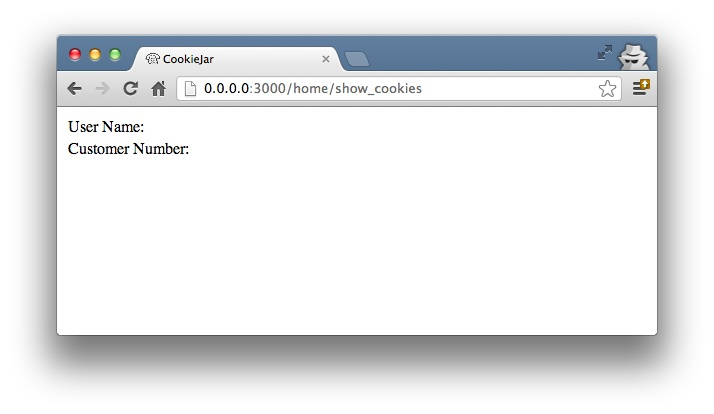
\includegraphics{screenshots/show_cookies_empty.jpg}
\end{figure}

Now go to the URL \texttt{http://0.0.0.0:3000/home/set\_cookies} and then back to \texttt{http://0.0.0.0:3000/home/show\_cookies}. Now you will see the values that we have set in the method \texttt{set\_cookies.}

\begin{figure}[htbp]
\centering
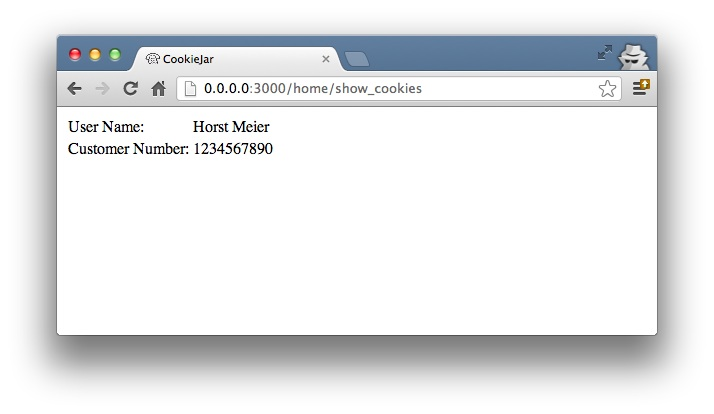
\includegraphics{screenshots/show_cookies_set.jpg}
\end{figure}

By requesting the page \texttt{http://0.0.0.0:3000/home/delete\_cookies} you can delete the cookies again.

\subsection{Note}\label{note-44}

The cookies you have placed in this way stay “alive” in the browser until you close the browser completely.

\subsection{Warning}\label{warning-12}

The content of a normally cookie in the browser is easy to read and to be manipulated by the user. It is not encrypted, so it should not contain any passwords or similar data. Nor is it advisable to save shopping baskets in an unsigned (see \hyperref[cookiesux5fsigned]{the section called “Signed Cookies)”}) cookie, otherwise the user could change the prices in this shopping basket himself.

\section{Permanent Cookies}\label{permanent-cookies}

Cookies are normally set to give the application a way of recognizing users when they visit again later. Between these visits to the website, much time can go by and the user may well close the browser in the meantime. To store cookies for longer than the current browser session, you can use the method \texttt{permanent}. Our above example can be expanded by adding this method in the \texttt{app/controllers/home\_controller.rb}:

\begin{shaded}\begin{verbatim}
class HomeController < ApplicationController
  def set_cookies
    cookies.permanent[:user_name]   = "Smith"
    cookies.permanent[:customer_number] = "1234567890"
  end

  def show_cookies
    @user_name    = cookies[:user_name]
    @customer_number = cookies[:customer_number]
  end

  def delete_cookies
    cookies.delete :user_name
    cookies.delete :customer_number
  end
end
\end{verbatim}\end{shaded}

\subsection{Important}\label{important-12}

“permanent” here does not really mean permanent. You cannot set a cookie permanently. When you set a cookie, it always needs a “valid until” stamp that the browser can use to automatically delete old cookies. With the method permanent this value is set to today's date in 20 years. This is practically the same as permanent.

\section{Signed Cookies)}\label{signed-cookies}

With normally placed cookies, you have no option on the application side to find out if the user of the application has changed the cookie. This can quickly lead to security problems, as changing the content of a cookie in the browser is no great mystery. The solution is signing the cookies with a key that is only known to us. This key is automatically created via a random generator with each \textbf{rails new} and is located in the file \texttt{config/initializers/secret\_token.rb}:

\begin{shaded}\begin{verbatim}
CookieJar::Application.config.secret_key_base = '85ec675d7702707667a25a'
\end{verbatim}\end{shaded}

\subsection{Warning}\label{warning-13}

If you want to set up your Rails application from scratch again one day and start over with a fresh Rails project, it can be helpful to transfer this key into the new Rails application. Otherwise you can no longer use the previously placed cookies!

To sign cookies, you can use the method \texttt{signed}. You have to use it for writing and reading the cookie. Our above example can be expanded by adding this method in the \texttt{app/controllers/home\_controller.rb}:

\begin{shaded}\begin{verbatim}
class HomeController < ApplicationController
  def set_cookies
    cookies.permanent.signed[:user_name]   = "Smith"
    cookies.permanent.signed[:customer_number] = "1234567890"
  end

  def show_cookies
    @user_name       = cookies.signed[:user_name]
    @customer_number = cookies.signed[:customer_number]
  end

  def delete_cookies
    cookies.delete :user_name
    cookies.delete :customer_number
  end
end
\end{verbatim}\end{shaded}

The content of the cookie is now saved in encrypted form every time you set the cookie. The name of the cookie can still be read by the user, but not the value.

\hyperdef{}{sessions}{\chap{Sessions}\label{sessions}}

As HTTP is a stateless protocol, we encounter special problems when developing applications. An individual web page has no connection to the next web page and they do not know of one another. But as you want to register only once on many websites, not over and over again on each individual page, this can pose a problem. The solution is called session and Rails offers it to the programmer transparently as a \texttt{session{[}{]}} hash. Rails automatically creates a new session for each new visitor of the web page. This session is saved by default as cookie (see \hyperref[cookies]{the section called “Cookies”}) and so it is subject to the 4 kB limit. But you can also store the sessions in the database (see \hyperref[sessionsux5fdatenbank]{the section called “Saving Sessions in the Database”}). An independent and unique session ID is created automatically and the cookie is deleted by default when the web browser is closed.

The beauty of a Rails session is that we can not just save strings there as with cookies, but also hashes and arrays. So you can for example use it to conveniently implement a shopping cart in an online shop.

\section{Breadcrumbs via Session}\label{breadcrumbs-via-session}

As an example, we create an application with a controller and three views. When a view is visited, the previously visited views are displayed in a little list.

The basic application:

\begin{shaded}\begin{verbatim}
$ rails new breadcrumbs
  [...]
$ cd breadcrumbs
$ rails generate controller Home ping pong index
  [...]
$
\end{verbatim}\end{shaded}

First we create a method with which we can save the last three URLs in the session and set an instance variable \texttt{@breadcrumbs,} to be able to neatly retrieve the values in the view. To that end, we set up a \texttt{before\_filter} in the \texttt{app/controllers/home\_controller.rb}:

\begin{shaded}\begin{verbatim}
class HomeController < ApplicationController
  before_filter :set_breadcrumbs

  def ping
  end

  def pong
  end

  def index
  end

  private
  def set_breadcrumbs
    if session[:breadcrumbs]
      @breadcrumbs = session[:breadcrumbs]
    else
      @breadcrumbs = Array.new
    end

    @breadcrumbs.push(request.url)

    if @breadcrumbs.count > 4
      ## shift removes the first element
      @breadcrumbs.shift
    end

    session[:breadcrumbs] = @breadcrumbs
  end
end
\end{verbatim}\end{shaded}

Now we use the \texttt{app/views/layouts/application.html.erb} to display these last entries at the top of each page:

\begin{shaded}\begin{verbatim}
<html>
<head>
  <title>Breadcrumbs</title>
  <%= stylesheet_link_tag    "application", media: "all", "data-turbolinks-track" => true %>
  <%= javascript_include_tag "application", "data-turbolinks-track" => true %>
  <%= csrf_meta_tags %>
</head>
<body>

<% if @breadcrumbs && @breadcrumbs.count > 1 %>
  <h3>Surf History</h3>
  <ul>
    <% @breadcrumbs[0..2].each do |breadcrumb| %>
      <li><%= link_to breadcrumb, breadcrumb %></li>
    <% end %>
  </ul>
<% end %>

<%= yield %>

</body>
</html>
\end{verbatim}\end{shaded}

Now you can start the Rails server with \textbf{rails server} and go to \texttt{http://0.0.0.0:3000/home/ping}, \texttt{http://0.0.0.0:3000/home/ping} or \texttt{http://0.0.0.0:3000/home/index} and at the top you will then always see the pages that you have visited before. Of course, this only works on the second page, because you do not yet have a history on the first page you visit.

\begin{figure}[htbp]
\centering
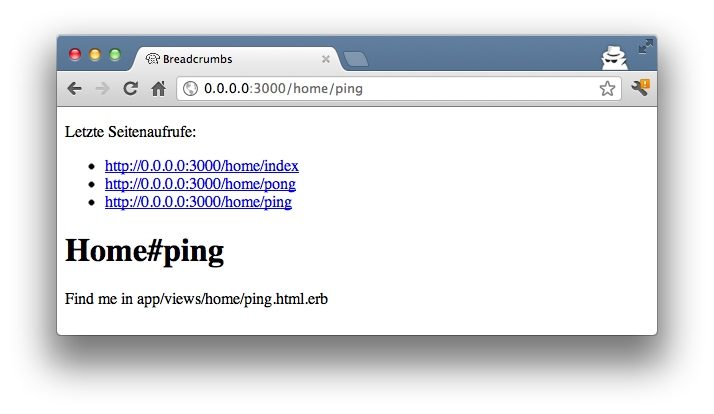
\includegraphics{screenshots/breadcrumbs_session_beispiel.jpg}
\end{figure}

\chap{reset\_session}\label{resetux5fsession}

Occasionally, there are situations where you want to reset a session (in other words, delete the current session and start again with a new, fresh session). For example, if you log out of a web application, the session will be reset. This is easily done and we can quickly integrate it into our breadcrumb application (see \hyperref[sessionux5fbreadcrumbs]{the section called “Breadcrumbs via Session”}):

\begin{shaded}\begin{verbatim}
$ rails generate controller Home reset -s
        skip  app/controllers/home_controller.rb
       route  get "home/reset"
      invoke  erb
       exist    app/views/home
      create    app/views/home/reset.html.erb
      invoke  test_unit
        skip    test/controllers/home_controller_test.rb
      invoke  helper
   identical    app/helpers/home_helper.rb
      invoke    test_unit
   identical      test/helpers/home_helper_test.rb
      invoke  assets
      invoke    coffee
   identical      app/assets/javascripts/home.js.coffee
      invoke    scss
   identical      app/assets/stylesheets/home.css.scss
$
\end{verbatim}\end{shaded}

The correspondingly expanded controller \texttt{app/controllers/home\_controller.rb} then looks like this:

\begin{shaded}\begin{verbatim}
class HomeController < ApplicationController
  before_filter :set_breadcrumbs

  def ping
  end

  def pong
  end

  def index
  end

  def reset
    reset_session
    @breadcrumbs = nil
  end

  private
  def set_breadcrumbs
    if session[:breadcrumbs]
      @breadcrumbs = session[:breadcrumbs]
    else
      @breadcrumbs = Array.new
    end

    @breadcrumbs.push(request.url)

    if @breadcrumbs.count > 4
      # shift removes the first element
      @breadcrumbs.shift
    end

    session[:breadcrumbs] = @breadcrumbs
  end
end
\end{verbatim}\end{shaded}

So you can delete the current session by going to the URL \texttt{http://0.0.0.0:3000/home/reset}.

\subsection{Note}\label{note-45}

It is not just important to invoke \texttt{reset\_session}, but you need to also set the instance variable \texttt{@breadcrumbs} to \texttt{nil}. Otherwise, the old breadcrumbs would still appear in the view..

\section{Saving Sessions in the Database}\label{saving-sessions-in-the-database}

Saving the entire session data in a cookie on the user's browser is not always the best solution. Amongst others, the limit of 4 kB can pose a problem. But it's no big obstacle, we can relocate the storing of the session from the cookie to the database with the Active Record Session Store gem (\texttt{https://github.com/rails/activerecord-session\_store}). Then the session ID is of course still saved in a cookie, but the whole other session data is stored in the database on the server.

To install the gem we have to add the following line at the end of the file \texttt{Gemfile}

\begin{shaded}\begin{verbatim}
gem 'activerecord-session_store', github: 'rails/activerecord-session_store'
\end{verbatim}\end{shaded}

After that we have to run \textbf{bundle install}

\begin{shaded}\begin{verbatim}
$ bundle install
Fetching git://github.com/rails/activerecord-session_store.git
remote: Counting objects: 134, done.
remote: Compressing objects: 100% (89/89), done.
remote: Total 134 (delta 48), reused 112 (delta 32)
Receiving objects: 100% (134/134), 24.33 KiB, done.
Resolving deltas: 100% (48/48), done.
Fetching gem metadata from https://rubygems.org/..........
Fetching gem metadata from https://rubygems.org/..
Resolving dependencies...
Using rake (10.1.0)
[...]
$
\end{verbatim}\end{shaded}

After that we have to run \textbf{rails generate active\_record:session\_migration} and \textbf{rake db:migrate} to create the needed table in the database.

\begin{shaded}\begin{verbatim}
$ rails generate active_record:session_migration
      create  db/migrate/20130717160101_add_sessions_table.rb
SW:breadcrumbs stefan$ rake db:migrate
==  AddSessionsTable: migrating ===============================================
-- create_table(:sessions)
   -> 0.0014s
-- add_index(:sessions, :session_id)
   -> 0.0003s
-- add_index(:sessions, :updated_at)
   -> 0.0004s
==  AddSessionsTable: migrated (0.0023s) ======================================

$
\end{verbatim}\end{shaded}

After that we'll have to change the \texttt{session\_store} in the file \texttt{config/initializers/session\_store.rb} to \texttt{:active\_record\_store}.

\begin{shaded}\begin{verbatim}
Breadcrumbs::Application.config.session_store :active_record_store
\end{verbatim}\end{shaded}

Job done. Now you need to start the server again with \textbf{rails server} and Rails saves all sessions in the database.

\chap{Action Mailer}\label{action-mailer}

Even if we mainly use Ruby on Rails to generate web pages, it sometimes is useful to be able to send an e-mail.

So let's go and build an example with minimal user management for a web shop that automatically sends an e-mail to the user when a new user is created:

\begin{shaded}\begin{verbatim}
$ rails new webshop
  [...]
$ cd webshop
$ rails generate scaffold User name email
  [...]
$ rake db:migrate
  [...]
$
\end{verbatim}\end{shaded}

For the user model we create a minimal validation in the \texttt{app/models/user.rb}, so that we can be sure that each user has a name and a syntactically correct e-mail address.

\begin{shaded}\begin{verbatim}
class User < ActiveRecord::Base
  validates :name,
            presence: true

  validates :email,
            presence: true,
            format: { with: /\A([^@\s]+)@((?:[-a-z0-9]+\.)+[a-z]{2,})\Z/i }
end
\end{verbatim}\end{shaded}

There is a generator with the name \texttt{mailer} that creates the files required for mailing. First, we have a look at the output of the \textbf{rails generate mailer}, without passing any further arguments:

\begin{shaded}\begin{verbatim}
$ rails generate mailer
Usage:
  rails generate mailer NAME [method method] [options]

Options:
      [--skip-namespace]        ## Skip namespace (affects only isolated applications)
  -e, [--template-engine=NAME]  # Template engine to be invoked
                                # Default: erb
  -t, [--test-framework=NAME]   # Test framework to be invoked
                                # Default: test_unit

Runtime options:
  -f, [--force]    # Overwrite files that already exist
  -p, [--pretend]  # Run but do not make any changes
  -q, [--quiet]    # Suppress status output
  -s, [--skip]     # Skip files that already exist

Description:
============
    Stubs out a new mailer and its views. Passes the mailer name, either
    CamelCased or under_scored, and an optional list of emails as arguments.

    This generates a mailer class in app/mailers and invokes your template
    engine and test framework generators.

Example:
========
    rails generate mailer Notifications signup forgot_password invoice

    creates a Notifications mailer class, views, and test:
        Mailer:     app/mailers/notifications.rb
        Views:      app/views/notifications/signup.text.erb [...]
        Test:       test/mailers/notifications_test.rb

$
\end{verbatim}\end{shaded}

That is just what we are expecting. So let's now create the mailer \texttt{notification}:

\begin{shaded}\begin{verbatim}
$ rails generate mailer Notification
      create  app/mailers/notification.rb
      invoke  erb
      create    app/views/notification
      invoke  test_unit
      create    test/mailers/notification_test.rb
$
\end{verbatim}\end{shaded}

In the file \texttt{app/mailers/notification.rb} you will find the controller:

\begin{shaded}\begin{verbatim}
class Notification < ActionMailer::Base
  default from: "from@example.com"
end
\end{verbatim}\end{shaded}

In it, we create a method \texttt{new\_account(user)}, with which we send the confirmation e-mail for a new account:

\begin{shaded}\begin{verbatim}
class Notification < ActionMailer::Base
  default from: "from@example.com"

  def new_account(user)
    @user = user
    mail(to: user.email,
         subject: "The account #{user.name} is active.")
  end
end
\end{verbatim}\end{shaded}

Now we create the view for this method. The file name \texttt{app/views/notification/new\_account.text.erb} is composed from the method name and the ending \texttt{text.erb}.

\begin{shaded}\begin{verbatim}
Hello <%= @user.name %>,

your new account is active.

Have a great day!
  A Robot
\end{verbatim}\end{shaded}

As we want to send this e-mail afer the create of a \texttt{User}, we still need add an \texttt{after\_create} callback which triggers the delivery. That is done in \texttt{app/models/user.rb}:

\begin{shaded}\begin{verbatim}
class User < ActiveRecord::Base
  validates :name,
            presence: true

  validates :email,
            presence: true,
            format: { with: /\A([^@\s]+)@((?:[-a-z0-9]+\.)+[a-z]{2,})\Z/i }

  after_create :send_welcome_email

  private

  def send_welcome_email
    Notification.new_account(self).deliver
  end
end
\end{verbatim}\end{shaded}

Let's create a new \texttt{User} in the console:

\begin{shaded}\begin{verbatim}
$ rails console
Loading development environment (Rails 4.0.0)
>> User.create(name: 'Wintermeyer', email: 'stefan.wintermeyer@amooma.de')
   (0.1ms)  begin transaction
  SQL (4.1ms)  INSERT INTO "users" ("created_at", "email", "name", "updated_at") VALUES (?, ?, ?, ?)  [["created_at", Wed, 17 Jul 2013 17:12:19 UTC +00:00], ["email", "stefan.wintermeyer@amooma.de"], ["name", "Wintermeyer"], ["updated_at", Wed, 17 Jul 2013 17:12:19 UTC +00:00]]
  Rendered notification/new_account.text.erb (0.8ms)

Sent mail to stefan.wintermeyer@amooma.de (11.1ms)
Date: Wed, 17 Jul 2013 19:12:20 +0200
From: from@example.com
To: stefan.wintermeyer@amooma.de
Message-ID: <51e6d07411000_a49d3fd87c8606d457513@SW.local.mail>
Subject: The account Wintermeyer is active.
Mime-Version: 1.0
Content-Type: text/plain;
 charset=UTF-8
Content-Transfer-Encoding: 7bit

Hello Wintermeyer,

your new account is active.

Have a great day!
  A Robot

   (2.9ms)  commit transaction
=> #<User id: 1, name: "Wintermeyer", email: "stefan.wintermeyer@amooma.de", created_at: "2013-07-17 17:12:19", updated_at: "2013-07-17 17:12:19">
>> exit
$
\end{verbatim}\end{shaded}

That was straightforward. In the development mode we see the e-mail in the log. In production mode it would be send to the configured SMTP gateway.

\section{Configuring the E-Mail Server}\label{configuring-the-e-mail-server}

Rails can use a local sendmail or an external SMTP server for delivering the e-mails.

\section{Sending via Local Sendmail}\label{sending-via-local-sendmail}

If you want to send the e-mails in the traditional way via local \texttt{sendmail}, then you need to insert the following lines into your configuration file \texttt{config/environments/development.rb} (for the development environment) or \texttt{config/environments/production.rb} (for your production environment):

\begin{shaded}\begin{verbatim}
config.action_mailer.delivery_method = :sendmail
config.action_mailer.perform_deliveries = true
config.action_mailer.raise_delivery_errors = true
\end{verbatim}\end{shaded}

\section{Sending via Direct SMTP}\label{sending-via-direct-smtp}

If you want to send the e-mail directly via a SMTP server (for example Google Mail), then you need to insert the following lines into your configuration file \texttt{config/environments/development.rb} (for the development environment) or \texttt{config/environments/production.rb} (for your production environment):

\begin{shaded}\begin{verbatim}
config.action_mailer.delivery_method = :smtp
config.action_mailer.smtp_settings = {
  address:              "smtp.gmail.com",
  port:                 587,
  domain:               'example.com',
  user_name:            '<username>',
  password:             '<password>',
  authentication:       'plain',
  enable_starttls_auto: true  }
\end{verbatim}\end{shaded}

Of course you need to adapt the values for \texttt{:domain}, \texttt{:user\_name} and \texttt{:password} in accordance with your configuration.

\section{Custom X-Header}\label{custom-x-header}

If you feel the urge to integrate an additional X-header then this is no problem. Here is an example for expanding the file \texttt{app/mailers/notification.rb}:

\begin{shaded}\begin{verbatim}
class Notification < ActionMailer::Base
  default from: "from@example.com"

  def new_account(user)
    @user = user
    headers["X-Priority"] = '3'
    mail(to: user.email,
         subject: "The new account #{user.name} is active.")
  end
end
\end{verbatim}\end{shaded}

This means the sent e-mail would look like this:

\begin{shaded}\begin{verbatim}
Sent mail to stefan.wintermeyer@amooma.de (50ms)
Date: Wed, 30 May 2012 17:35:21 +0200
From: from@example.com
To: stefan.wintermeyer@amooma.de
Message-ID: <4fc63e39e356a_aa083fe366028cd8803c7@MacBook.local.mail>
Subject: The new account Wintermeyer is active.
Mime-Version: 1.0
Content-Type: text/plain;
 charset=UTF-8
Content-Transfer-Encoding: 7bit
X-Priority: 3

Hello Wintermeyer,

your new account is active.

Have a great day!
  A Robot
\end{verbatim}\end{shaded}

\section{HTML E-Mails}\label{html-e-mails}

Creating HTML e-mails is really easy. Please create the file \texttt{app/views/user\_mailer/new\_account\_email.html.erb} with the following content:

\begin{shaded}\begin{verbatim}
<!DOCTYPE html>
<html>
  <head>
    <meta content="text/html; charset=UTF-8" http-equiv="Content-Type" />
  </head>
  <body>
    <p>Hello <%= @user.name %>,</p>

    <p>your new account is active.</p>

    <p><i>Have a great day!</i></p>
    <p>A Robot</p>
  </body>
</html>
\end{verbatim}\end{shaded}

If you now create a user, the log file \texttt{log/development.log} will show you what was rendered and the e-mail that was sent:

\begin{shaded}\begin{verbatim}
  Rendered notification/new_account.html.erb (2.0ms)
  Rendered notification/new_account.text.erb (0.4ms)

Sent mail to stefan.wintermeyer@amooma.de (69ms)
Date: Wed, 30 May 2012 17:46:49 +0200
From: from@example.com
To: stefan.wintermeyer@amooma.de
Message-ID: <4fc640e930bff_aa173fd61d828ce0501e4@MacBook.local.mail>
Subject: The new account Wintermeyer is active.
Mime-Version: 1.0
Content-Type: multipart/alternative;
 boundary="--==_mimepart_4fc640e921794_aa173fd61d828ce04987d";
 charset=UTF-8
Content-Transfer-Encoding: 7bit



----==_mimepart_4fc640e921794_aa173fd61d828ce04987d
Date: Wed, 30 May 2012 17:46:49 +0200
Mime-Version: 1.0
Content-Type: text/plain;
 charset=UTF-8
Content-Transfer-Encoding: 7bit
Content-ID: <4fc640e926312_aa173fd61d828ce04998e@MacBook.local.mail>

Hello Wintermeyer,

your new account is active.

Have a great day!
  A Robot

----==_mimepart_4fc640e921794_aa173fd61d828ce04987d
Date: Wed, 30 May 2012 17:46:49 +0200
Mime-Version: 1.0
Content-Type: text/html;
 charset=UTF-8
Content-Transfer-Encoding: 7bit
Content-ID: <4fc640e928055_aa173fd61d828ce0500ea@MacBook.local.mail>

<!DOCTYPE html>
<html>
  <head>
    <meta content="text/html; charset=UTF-8" http-equiv="Content-Type" />
  </head>
  <body>
    <p>Hello Wintermeyer,</p>

    <p>your new account is active.</p>

    <p><i>Have a great day!</i></p>
    <p>A Robot</p>
  </body>
</html>

----==_mimepart_4fc640e921794_aa173fd61d828ce04987d--
\end{verbatim}\end{shaded}

Rails has automatically generated an e-mail in the MIME format \texttt{multipart/alternative}, as the view was present both in the format \texttt{html.erb} and \texttt{text.erb}.

\section{Attachments}\label{attachments}

E-mail attachments are also defined in the controller.

As an example we add in \texttt{app/mailers/notification.rb} the Rails image \texttt{app/assets/images/rails.png} to an e-mail as attachment:

\begin{shaded}\begin{verbatim}
class Notification < ActionMailer::Base
  default from: "from@example.com"

  def new_account(user)
    @user = user
    attachments['rails.png'] = File.read("#{Rails.root}/app/assets/images/rails.png")
    mail(to: user.email,
         subject: "The new account #{user.name} is active.")
  end
end
\end{verbatim}\end{shaded}

\chap{Inline Attachments}\label{inline-attachments}

For \emph{inline attachments} in HTML e-mails, you need to use the method \texttt{inline} when calling \texttt{attachments}. In our example controller \texttt{app/mailers/notification.rb}:

\begin{shaded}\begin{verbatim}
class Notification < ActionMailer::Base
  default from: "from@example.com"

  def new_account(user)
    @user = user
    attachments.inline['rails.png'] = File.read("#{Rails.root}/app/assets/images/rails.png")
    mail(to: user.email,
         subject: "The new account #{user.name} is active.")
  end
end
\end{verbatim}\end{shaded}

In the HTML e-mail, you can access the hash \texttt{attachments{[}{]}} via \texttt{image\_tag}. In our example the \texttt{app/views/notification/new\_account.html.erb} would look like this:

\begin{shaded}\begin{verbatim}
<!DOCTYPE html>
<html>
  <head>
    <meta content="text/html; charset=UTF-8" http-equiv="Content-Type" />
  </head>
  <body>
    <%= image_tag attachments['rails.png'].url, :alt => 'Rails Logo' %>
    <p>Hello <%= @user.name %>,</p>

    <p>your new account is active.</p>

    <p><i>Have a great day!</i></p>
    <p>A Robot</p>
  </body>
</html>
\end{verbatim}\end{shaded}

\chap{Further Information}\label{further-information}

The Rails online documentation has a very extensive entry on ActionMailer at \url{http://guides.rubyonrails.org/action_mailer_basics.html}\{.uri\}.

Ryan Bates offers an excellent screencast about this topic at \url{http://railscasts.com/episodes/206-action-mailer-in-rails-3}\{.uri\}.

\chap{Internationalization}\label{internationalization}

\section{Introduction}\label{introduction-4}

If you are in the lucky situation of only creating web pages in English, then you can skip this chapter completely. For you, everything is set up correctly by default. But even if you want to create a web page that only uses one language (other than English), you will need to dive into this chapter. It is not enough to just translate the views. Because already if you use scaffolding, you will need to take care of the English and therefore not yet translated validation errors.

The class \texttt{I18n} is responsible for anything to do with translation in the Rails application. It offers two important methods for this purpose:

\begin{itemize}
\itemsep1pt\parskip0pt\parsep0pt
\item
  \texttt{I18n.translate} or \texttt{I18n.t} Takes care of inserting previously defined text blocks. These can contain variables.
\item
  \texttt{I18n.localize} or \texttt{I18n.l} Takes care of adapting time and date specifications to the local format.
\end{itemize}

With \texttt{I18n.locale} you define the language you want to use in the current call. In the configuration file \texttt{config/application.rb}, the entry \texttt{config.i18n.default\_locale} sets the default value for \texttt{I18n.locale}. If you do not make any changes there, this value is set by default to \texttt{:en} for English.

For special cases such as displaying numbers, currencies and times, there are special helpers available. For example, if you want to create a German web page, you can ensure that the number 1000.23 can be correctly displayed with a decimal comma as “1.000,23” on the German page and with a decimal point on an English web page as “1,000.23”.

Let's create an example application which includes the rails-i18n gem by Sven Fuchs (\texttt{https://github.com/svenfuchs/i18n}). The gem provides a couple of language files with translations and format info.

\begin{shaded}\begin{verbatim}
$ rails new webshop
  [...]
$ cd webshop
$ echo "gem 'rails-i18n'" >> Gemfile
$ bundle install
  [...]
$
\end{verbatim}\end{shaded}

In the console we can see the different output of a number depending on the language setting:

\begin{shaded}\begin{verbatim}
$ rails console
Loading development environment (Rails 4.0.0)
>> price = 1000.23
=> 1000.23
>> helper.number_to_currency(price, locale: :de)
=> "1.000,23 €"
>> helper.number_to_currency(price, locale: :en)
=> "$1,000.23"
>> helper.number_to_currency(price, locale: :fr)
=> "1 000,23 €"
>> exit
$
\end{verbatim}\end{shaded}

You see it is not just about translating some views.

\chap{I18n.t}\label{i18n.t}

With \texttt{I18n.t} you can retrieve previously defined translations. The translations are saved by default in YAML format in the directory \texttt{config/locales/}. Technically, you do not have to use YAML as format.

In \texttt{config/locales/} you can find an example file \texttt{config/locales/en.yml} with the following content:

\begin{shaded}\begin{verbatim}
en:
  hello: "Hello world"
\end{verbatim}\end{shaded}

In the Rails console we can try out how \texttt{I18n.t} works:

\begin{shaded}\begin{verbatim}
$ rails console
Loading development environment (Rails 4.0.0)
>> I18n.t :hello
=> "Hello world"
>> I18n.locale
=> :en
>> exit
$
\end{verbatim}\end{shaded}

Let's first create a \texttt{config/locales/de.yml} with the following content:

\begin{shaded}\begin{verbatim}
de:
  hello: "Hallo Welt"
\end{verbatim}\end{shaded}

In the console we can set the system language with \texttt{I18n.locale = :de} to German.

\begin{shaded}\begin{verbatim}
$ rails console
Loading development environment (Rails 4.0.0)
>> I18n.locale
=> :en
>> I18n.locale = :de
=> :de
>> I18n.t :hello
=> "Hallo Welt"
>>
\end{verbatim}\end{shaded}

\texttt{I18n.t} looks by default for the entry in the language defined in \texttt{I18n.locale}. It does not matter if you are working with \texttt{I18n.t} or \texttt{I18n.translate}. Nor does it matter if you are searching for a symbol or a string:

\begin{shaded}\begin{verbatim}
>> I18n.locale = :en
=> :en
>> I18n.t :hello
=> "Hello world"
>> I18n.t 'hello'
=> "Hello world"
>> I18n.translate 'hello'
=> "Hello world"
>>
\end{verbatim}\end{shaded}

If a translation does not exist, you get an error message that says “\texttt{translation missing:}”. This also applies if a translation is only missing in one language (then all other languages will work, but for the missing translation you will get the error message). In that case, you can define a default with \texttt{:default       =\textgreater{} 'any default value'}:

\begin{shaded}\begin{verbatim}
>> I18n.t 'asdfasdfasdf'
=> "translation missing: en.asdfasdfasdf"
>> I18n.t 'asdfasdfasdf', :default => 'asdfasdfasdf'
=> "asdfasdfasdf"
>> exit
$
\end{verbatim}\end{shaded}

In the YAML structure you can also specify several levels. Please amend the \texttt{config/locale/en.yml} as follows:

\begin{shaded}\begin{verbatim}
en:
  hello: "Hello world"
  example:
    test: "A test"
  aaa:
    bbb:
      test: "An other test"
\end{verbatim}\end{shaded}

You can display the different levels within the string with dots or with a \texttt{:scope} for the symbols. You can also mix both options.

\begin{shaded}\begin{verbatim}
$ rails console
Loading development environment (Rails 4.0.0)
>> I18n.t 'example.test'
=> "A test"
>> I18n.t 'aaa.bbb.test'
=> "An other test"
>> I18n.t :test, scope: [:aaa, :bbb]
=> "An other test"
>> I18n.t :test, scope: 'aaa.bbb'
=> "An other test"
>> exit
$
\end{verbatim}\end{shaded}

It is up to you which structure you choose to save your translations in the YAML files. But the structure described in \hyperref[i18nux5feinsprachigux5fdeutsch]{the section called “A Rails Application in Only One Language: German”} does make some things easier and that's why we are going to use it for this application as well.

\section{Using I18n.t in the View}\label{using-i18n.t-in-the-view}

In the view, you can use \texttt{I18n.t} as follows:

\begin{shaded}\begin{verbatim}
<%= t :hello-world %>

<%= I18n.t :hello-world %>

<%= I18n.translate :hello-world %>

<%= I18n.t 'hello-world' %>

<%= I18n.t 'aaa.bbb.test' %>

<%= link_to I18n.t('views.destroy'), book, confirm: I18n.t('views.are_you_sure'), method: :delete %>
\end{verbatim}\end{shaded}

\section{Localized Views}\label{localized-views}

In Rails, there is a useful option of saving several variations of a view as “localized views”, each of which represents a different language. This technique is independent of the potential use of \texttt{I18n.t} in these views. The file name results from the view name, the language code (for example, \texttt{de} for German) and \texttt{html.erb} for ERB pages. Each of these are separated by a dot. So the German variation of the \texttt{index.html.erb} page would get the file name \texttt{index.de.html.erb}.

Your views directory could then look like this:

\begin{shaded}\begin{verbatim}
|-app
|---views
|-----products
|-------_form.html.erb
|-------_form.de.html.erb
|-------edit.html.erb
|-------edit.de.html.erb
|-------index.html.erb
|-------index.de.html.erb
|-------new.html.erb
|-------new.de.html.erb
|-------show.html.erb
|-------show.de.html.erb
|-------
|-----page
|-------index.html.erb
|-------index.de.html.erb
\end{verbatim}\end{shaded}

The language set with \texttt{config.i18n.default\_locale} is used automatically if no language was encoded in the file name. In a new and not yet configured Rails project, this will be English. You can configure it in the file \texttt{config/application.rb}.

\chap{A Rails Application in Only One Language: German}\label{a-rails-application-in-only-one-language-german}

In a Rails application aimed only at German users, it is unfortunately not enough to just translate all the views into German. The approach is in many respects similar to a multi-lingual Rails application (see \hyperref[i18nux5fmehrsprachigeux5frailsux5fapplikation]{the section called “Multilingual Rails Application”}). Correspondingly, there will be a certain amount of repetition. I am going to show you the steps you need to watch out for by using a simple application as example.

Let's go through all the changes using the example of this bibliography application:

\begin{shaded}\begin{verbatim}
$ rails new bibliography
  [...]
$ cd bibliography
$ rails generate scaffold book title number_of_pages:integer 'price:decimal{7,2}'
  [...]
$ rake db:migrate
  [...]
$
\end{verbatim}\end{shaded}

To get examples for validation errors, please insert the following validations in the \texttt{app/models/book.rb}:

\begin{shaded}\begin{verbatim}
class Book < ActiveRecord::Base
  validates :title,
            presence: true,
            uniqueness: true,
            length: { within: 2..255 }

  validates :price,
            presence: true,
            numericality: { greater_than: 0 }
end
\end{verbatim}\end{shaded}

Please search the configuration file \texttt{config/application.rb} for the value \texttt{config.i18n.default\_locale} and set it to \texttt{:de} for German. In the same context, we then also insert two directories in the line above for the translations of the models and the views. This directory structure is not a technical requirement, but makes it easier to keep track of things if your application becomes big:

\begin{shaded}\begin{verbatim}
config.i18n.load_path += Dir[Rails.root.join('config', 'locales', 'models', '*', '*.yml').to_s]
config.i18n.load_path += Dir[Rails.root.join('config', 'locales', 'views', '*', '*.yml').to_s]
config.i18n.default_locale = :de
\end{verbatim}\end{shaded}

You then still need to create the corresponding directories:

\begin{shaded}\begin{verbatim}
$ mkdir -p config/locales/models/book
$ mkdir -p config/locales/views/book
$
\end{verbatim}\end{shaded}

Now you need to generate a language configuration file for German or simply download a ready-made one by Sven Fuchs from his Github repository at \texttt{https://github.com/svenfuchs/rails-i18n}:

\begin{shaded}\begin{verbatim}
$ cd config/locales
$ curl -O https://raw.github.com/svenfuchs/rails-i18n/master/rails/locale/de.yml
  % Total    % Received % Xferd  Average Speed   Time    Time     Time  Current
                                 Dload  Upload   Total   Spent    Left  Speed
100  4940  100  4940    0     0   4296      0  0:00:01  0:00:01 --:--:--  4862
$
\end{verbatim}\end{shaded}

\section{Note}\label{note-46}

If you know how Bundler works, you can also insert the line \texttt{gem 'rails-i18n'} into the file \texttt{Gemfile} and then execute \textbf{bundle install}. This gives you all language files from the repository.

In the file \texttt{config/locales/de.yml}, you have all required formats and generic wordings for German that you need for a normal Rails application (for example, days of the week, currency symbols, etc). Have a look at it with your favorite editor to get a first impression.

Next, we need to tell Rails that a model `book' is not called `book' in German, but `Buch'. The same applies to all attributes. So we create the file \texttt{config/locales/models/book/de.yml} with the following structure. As side effect, we get the methods \texttt{Model.model\_name.human} and \texttt{Model.human\_attribute\_name(attribute)}, with which we can insert the model and attribute names in the view.

\begin{shaded}\begin{verbatim}
de:
  activerecord:
    models:
      book: 'Buch'
    attributes:
      book:
        title: 'Titel'
        number_of_pages: 'Seitenanzahl'
        price: 'Preis'
\end{verbatim}\end{shaded}

In the file \texttt{config/locales/views/book/de.yml} we insert a few values for the scaffold views:

\begin{shaded}\begin{verbatim}
de:
  views:
    show: Anzeigen
    edit: Editieren
    destroy: Löschen
    are_you_sure: Sind Sie sicher?
    back: Zurück
    edit: Editieren
    book:
      index:
        title: Bücherliste
        new: Neues Buch
      edit:
        title: Buch editieren
      new:
        title: Neues Buch
      flash_messages:
        book_was_successfully_created: 'Das Buch wurde erfolgreich angelegt.'
        book_was_successfully_updated: 'Das Buch wurde erfolgreich aktualisiert.'
\end{verbatim}\end{shaded}

Now we still need to integrate a “few” changes into the views. We use the \texttt{I18n.t} helper that can also be abbreviated with \texttt{t} in the view. \texttt{I18n.t} reads out the corresponding item from the YAML file. In the case of a purely monolingual German application, we could also write the German text directly into the view, but with this method we can more easily switch to multilingual use if required. You can find more information on I18n.t in \hyperref[i18nux5fi18nux5ft]{the section called “I18n.t”}.

\texttt{app/views/books/\_form.html.erb}

\begin{shaded}\begin{verbatim}
<%= form_for(@book) do |f| %>
  <% if @book.errors.any? %>
    <div id="error_explanation">
      <h2><%= t 'activerecord.errors.template.header', :model => Book.model_name.human, :count => @book.errors.count %></h2>
      <ul>
      <% @book.errors.full_messages.each do |msg| %>
        <li><%= msg %></li>
      <% end %>
      </ul>
    </div>
  <% end %>

  <div class="field">
    <%= f.label :title %><br>
    <%= f.text_field :title %>
  </div>
  <div class="field">
    <%= f.label :number_of_pages %><br>
    <%= f.number_field :number_of_pages %>
  </div>
  <div class="field">
    <%= f.label :price %><br>
    <%= f.text_field :price %>
  </div>
  <div class="actions">
    <%= f.submit %>
  </div>
<% end %>
\end{verbatim}\end{shaded}

\texttt{app/views/books/edit.html.erb}

\begin{shaded}\begin{verbatim}
<h1><%= t 'views.book.edit.title' %></h1>

<%= render 'form' %>

<%= link_to I18n.t('views.show'), @book %> |
<%= link_to I18n.t('views.back'), books_path %>
\end{verbatim}\end{shaded}

\texttt{app/views/books/index.html.erb}

\begin{shaded}\begin{verbatim}
<h1><%= t 'views.book.index.title' %></h1>

<table>
  <thead>
    <tr>
      <th><%= Book.human_attribute_name(:title) %></th>
      <th><%= Book.human_attribute_name(:number_of_pages) %></th>
      <th><%= Book.human_attribute_name(:price) %></th>
      <th></th>
      <th></th>
      <th></th>
    </tr>
  </thead>

  <tbody>
    <% @books.each do |book| %>
      <tr>
        <td><%= book.title %></td>
        <td><%= number_with_delimiter(book.number_of_pages) %></td>
        <td><%= number_to_currency(book.price) %></td>
        <td><%= link_to I18n.t('views.show'), book %></td>
        <td><%= link_to I18n.t('views.edit'), edit_book_path(book) %></td>
        <td><%= link_to I18n.t('views.destroy'), book, method: :delete, data: { confirm: I18n.t('views.are_you_sure')} %></td>
      </tr>
    <% end %>
  </tbody>
</table>

<br>

<%= link_to I18n.t('views.book.index.new'), new_book_path %>
\end{verbatim}\end{shaded}

\texttt{app/views/books/new.html.erb}

\begin{shaded}\begin{verbatim}
<h1><%= t 'views.book.new.title' %></h1>

<%= render 'form' %>

<%= link_to I18n.t('views.back'), books_path %>
\end{verbatim}\end{shaded}

\texttt{app/views/books/show.html.erb}

\begin{shaded}\begin{verbatim}
<p id="notice"><%= notice %></p>

<p>
  <strong><%= Book.human_attribute_name(:title) %>:</strong>
  <%= @book.title %>
</p>

<p>
  <strong><%= Book.human_attribute_name(:number_of_pages) %>:</strong>
  <%= number_with_delimiter(@book.number_of_pages) %>
</p>

<p>
  <strong><%= Book.human_attribute_name(:price) %>:</strong>
  <%= number_to_currency(@book.price) %>
</p>

<%= link_to I18n.t('views.edit'), edit_book_path(@book) %> |
<%= link_to I18n.t('views.back'), books_path %>
\end{verbatim}\end{shaded}

\subsection{Note}\label{note-47}

In the show and index view, I have integrated the helpers \texttt{number\_with\_delimiter} and \texttt{number\_to\_currency} so the numbers are represented more attractively for the user.

Right at the end, we still need to adapt a few flash messages in the controller \texttt{app/controllers/books\_controller.rb}:

\begin{shaded}\begin{verbatim}
class BooksController < ApplicationController
  before_action :set_book, only: [:show, :edit, :update, :destroy]

  ## GET /books
  # GET /books.json
  def index
    @books = Book.all
  end

  # GET /books/1
  # GET /books/1.json
  def show
  end

  # GET /books/new
  def new
    @book = Book.new
  end

  # GET /books/1/edit
  def edit
  end

  # POST /books
  # POST /books.json
  def create
    @book = Book.new(book_params)

    respond_to do |format|
      if @book.save
        format.html { redirect_to @book, notice: I18n.t('views.book.flash_messages.book_was_successfully_created') }
        format.json { render action: 'show', status: :created, location: @book }
      else
        format.html { render action: 'new' }
        format.json { render json: @book.errors, status: :unprocessable_entity }
      end
    end
  end

  # PATCH/PUT /books/1
  # PATCH/PUT /books/1.json
  def update
    respond_to do |format|
      if @book.update(book_params)
        format.html { redirect_to @book, notice: I18n.t('views.book.flash_messages.book_was_successfully_updated') }
        format.json { head :no_content }
      else
        format.html { render action: 'edit' }
        format.json { render json: @book.errors, status: :unprocessable_entity }
      end
    end
  end

  # DELETE /books/1
  # DELETE /books/1.json
  def destroy
    @book.destroy
    respond_to do |format|
      format.html { redirect_to books_url }
      format.json { head :no_content }
    end
  end

  private
    # Use callbacks to share common setup or constraints between actions.
    def set_book
      @book = Book.find(params[:id])
    end

    # Never trust parameters from the scary internet, only allow the white list through.
    def book_params
      params.require(:book).permit(:title, :number_of_pages, :price)
    end
end
\end{verbatim}\end{shaded}

Now you can use the views generated by the scaffold generator entirely in German. The structure of the YAML files shown here can of course be adapted to your own preferences. The texts in the views and the controller are displayed with \texttt{I18n.t}. At this point you could of course also integrate the German text directly if the application is purely in German.

\chap{Paths in German}\label{paths-in-german}

Our bibliography is completely in German, but the URLs are still in English. If we want to make all books available at the URL \texttt{http://0.0.0.0:3000/buecher} instead of the URL \texttt{http://0.0.0.0:3000/books} then we need to add the following entry to the \texttt{config/routes.rb}:

\begin{shaded}\begin{verbatim}
Bibliography::Application.routes.draw do
  resources :books, path: 'buecher', path_names: { new: 'neu', edit: 'editieren' }
end
\end{verbatim}\end{shaded}

As a result, we then have the following new paths:

\begin{shaded}\begin{verbatim}
$ rake routes
   Prefix Verb   URI Pattern                      Controller#Action
    books GET    /buecher(.:format)               books#index
          POST   /buecher(.:format)               books#create
 new_book GET    /buecher/neu(.:format)           books#new
edit_book GET    /buecher/:id/editieren(.:format) books#edit
     book GET    /buecher/:id(.:format)           books#show
          PATCH  /buecher/:id(.:format)           books#update
          PUT    /buecher/:id(.:format)           books#update
          DELETE /buecher/:id(.:format)           books#destroy
$
\end{verbatim}\end{shaded}

The brilliant thing with Rails routes is that you do not need to do anything else. The rest is managed transparently by the routing engine.

\chap{Multilingual Rails Application}\label{multilingual-rails-application}

The approach for multilingual Rails applications is very similar to the monoligual, all-German Rails application described in \hyperref[i18nux5feinsprachigux5fdeutsch]{the section called “A Rails Application in Only One Language: German”}. But we need to define YAML language files for all required languages and tell the Rails application which language it should currently use. We do this via \texttt{I18n.locale}.

\chap{Using I18n.locale for Defining the Default Language}\label{using-i18n.locale-for-defining-the-default-language}

Of course, a Rails application has to know in which language a web page should be represented. \texttt{I18n.locale} saves the current language and can be read by the application. I am going to show you this with a mini web shop example:

\begin{shaded}\begin{verbatim}
$ rails new webshop
  [...]
$ cd webshop
$
\end{verbatim}\end{shaded}

This web shop gets a homepage:

\begin{shaded}\begin{verbatim}
$ rails generate controller Page index
  [...]
$
\end{verbatim}\end{shaded}

We still need to enter it as root page in the \texttt{config/routes.rb}:

\begin{shaded}\begin{verbatim}
Webshop::Application.routes.draw do
  get "page/index"
  root 'page#index'
end
\end{verbatim}\end{shaded}

We populate the \texttt{app/views/page/index.html.erb} with the following example:

\begin{shaded}\begin{verbatim}
<h1>Example Webshop</h1>
<p>Welcome to this webshop.</p>

<p>
<strong>I18n.locale:</strong>
<%= I18n.locale %>
</p>
\end{verbatim}\end{shaded}

If we start the Rails server with \textbf{rails server} and go to \texttt{http://0.0.0.0:3000/} in the browser, then we see the following web page:

\begin{figure}[htbp]
\centering
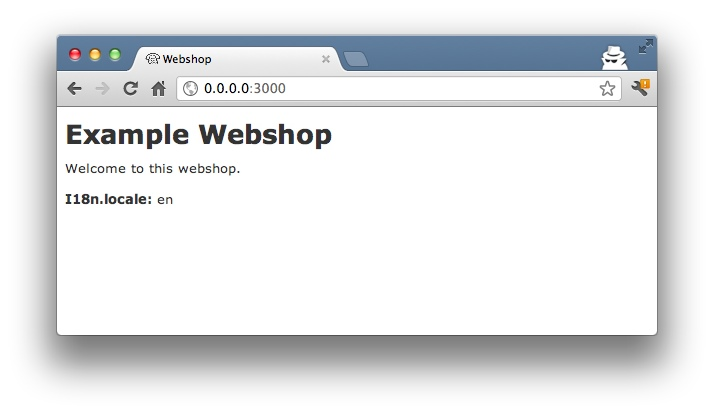
\includegraphics{screenshots/i18n_ganze_seite_page_index.jpg}
\end{figure}

As you can see, the default is set to “en” for English. Stop the Rails server with \textbf{CTRL-C} and change the setting for the default language to German in the file \texttt{config/application.rb}:

\begin{shaded}\begin{verbatim}
config.i18n.default_locale = :de
\end{verbatim}\end{shaded}

If you then start the Rails server and again go to \texttt{http://0.0.0.0:3000/} in the web browser, you will see the following web page:

\begin{figure}[htbp]
\centering
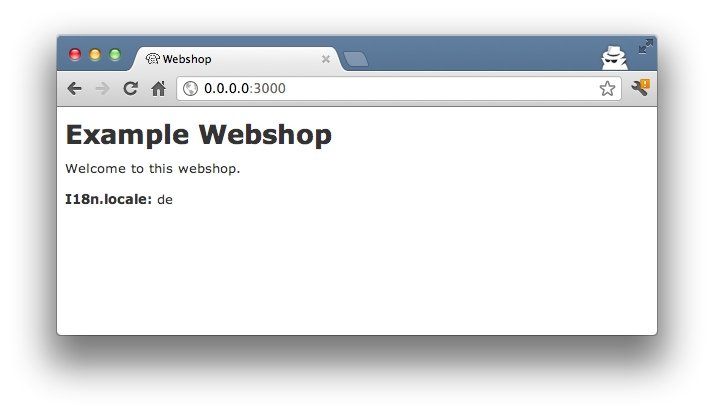
\includegraphics{screenshots/i18n_ganze_seite_page_index_default_locale_de.jpg}
\end{figure}

The web page has not changed, but as output of \texttt{\textless{}\%=       I18n.locale \%\textgreater{}} you now get `\texttt{de}' for German (Deutsch), not `\texttt{en}' for English as before.

Please stop the Rails server with \textbf{CTRL-C} and change the setting for the default language to \texttt{en} for English in the file \texttt{config/application.rb}:

\begin{shaded}\begin{verbatim}
## The default locale is :en and all translations from config/locales/*.rb,yml are auto loaded.
## config.i18n.load_path += Dir[Rails.root.join('my', 'locales', '*.{rb,yml}').to_s]

config.i18n.default_locale = :en
\end{verbatim}\end{shaded}

We now know how to set the default for \texttt{I18n.locale} in the entire application, but that only gets half the job done. A user wants to be able to choose his own language. There are various ways of achieving this. To make things clearer, we need a second page that displays a German text.

Please create the file \texttt{app/views/page/index.de.html.erb} with the following content:

\begin{shaded}\begin{verbatim}
<h1>Beispiel Webshop</h1>
<p>Willkommen in diesem Webshop.</p>

<p>
<strong>I18n.locale:</strong>
<%= I18n.locale %>
</p>
\end{verbatim}\end{shaded}

\chap{Setting I18n.locale via URL Path Prefix}\label{setting-i18n.locale-via-url-path-prefix}

The more stylish way of setting the language is to add it as prefix to the URL. This enables search engines to manage different language versions better. We want \texttt{http://0.0.0.0:3000/de} to display the German version of our homepage and \texttt{http://0.0.0.0:3000/en} the English version. The first step is adapting the \texttt{config/routes.rb}

\begin{shaded}\begin{verbatim}
Webshop::Application.routes.draw do
  scope ':locale', locale: /en|de/ do
    get "page/index"
    get '/', to: 'page#index'
  end

  root 'page#index'
end
\end{verbatim}\end{shaded}

Next, we need to set a \texttt{before\_filter} in the \texttt{app/controllers/application\_controller.rb}. This filter sets the parameter locale set by the route as \texttt{I18n.locale}:

\begin{shaded}\begin{verbatim}
class ApplicationController < ActionController::Base
  # Prevent CSRF attacks by raising an exception.
  # For APIs, you may want to use :null_session instead.
  protect_from_forgery with: :exception

  before_filter :set_locale

  private
  def set_locale
    I18n.locale = params[:locale] || I18n.default_locale
  end
end
\end{verbatim}\end{shaded}

To test it, start Rails with \textbf{rails server} and go to the URL \texttt{http://0.0.0.0:3000/de}.

\begin{figure}[htbp]
\centering
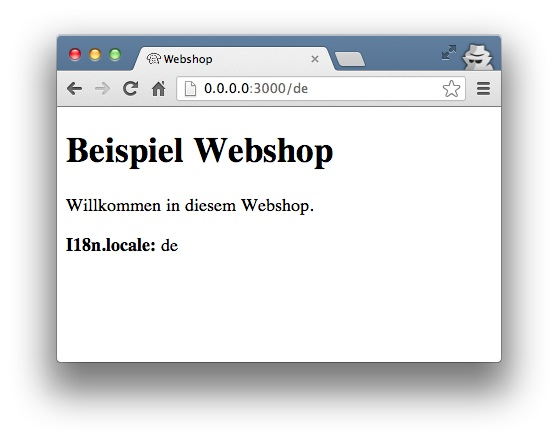
\includegraphics{screenshots/i18n_path_prefix_de_root.jpg}
\end{figure}

Of course we can also go to \texttt{http://0.0.0.0:3000/de/page/index}:

\begin{figure}[htbp]
\centering
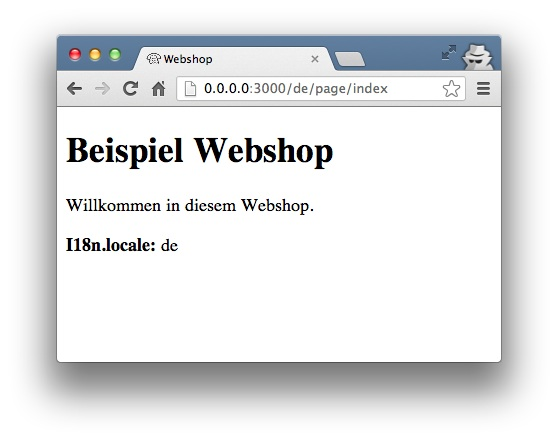
\includegraphics{screenshots/i18n_path_prefix_de_page_index.jpg}
\end{figure}

If we go to \texttt{http://0.0.0.0:3000/en} and \texttt{http://0.0.0.0:3000/en/page/index} we get the English version of each page.

But now we have a problem: by using the prefix, we initially get to a page with the correct language, but what if we want to link from that page to another page in our Rails project? Then we would need to manually insert the prefix into the link. Who wants that? Obviously there is a clever solution for this problem. We can set global default parameters for URL generation by defining a method called \texttt{default\_url\_options} in our controller.

So we just need to add this method in \texttt{app/controllers/application\_controller.rb}:

\begin{shaded}\begin{verbatim}
class ApplicationController < ActionController::Base
  # Prevent CSRF attacks by raising an exception.
  # For APIs, you may want to use :null_session instead.
  protect_from_forgery with: :exception

  before_filter :set_locale

  def default_url_options
    { locale: I18n.locale }
  end

  private
  def set_locale
    I18n.locale = params[:locale] || I18n.default_locale
  end
end
\end{verbatim}\end{shaded}

As a result, all links created with \texttt{link\_to} and \texttt{url\_for} (on which \texttt{link\_to} is based) are automatically expanded by the parameter \texttt{locale}. You do not need to do anything else. All links generated via the scaffold generator are automatically changed accordingly.

\section{Navigation Example}\label{navigation-example}

To give the user the option of switching easily between the different language versions, it makes sense to offer two links at the top of the web page. We don't want the current language to be displayed as active link. This can be achieved as follows for all views in the file \texttt{app/views/layouts/application.html.erb}:

\begin{shaded}\begin{verbatim}
<!DOCTYPE html>
<html>
<head>
  <title>Webshop</title>
  <%= stylesheet_link_tag    "application", media: "all", "data-turbolinks-track" => true %>
  <%= javascript_include_tag "application", "data-turbolinks-track" => true %>
  <%= csrf_meta_tags %>
</head>
<body>

<p>
<%= link_to_unless I18n.locale == :en, "English", locale: :en %>
|
<%= link_to_unless I18n.locale == :de, "Deutsch", locale: :de %>
</p>

<%= yield %>

</body>
</html>
\end{verbatim}\end{shaded}

The navigation is then displayed at the top of the page.

\begin{figure}[htbp]
\centering
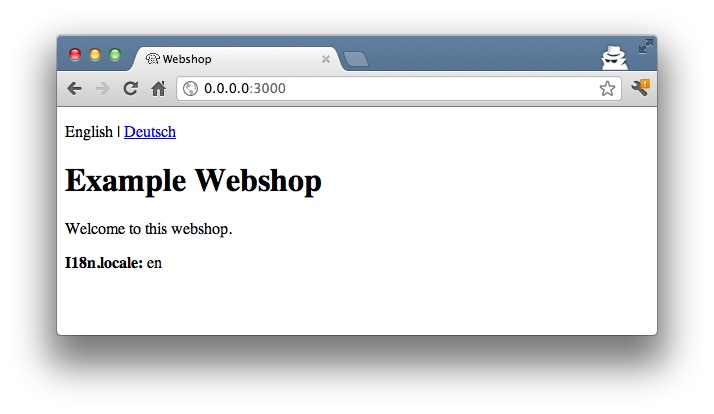
\includegraphics{screenshots/I18n_locale_url_prefix_navigation.jpg}
\end{figure}

\section{Setting I18n.locale via Accept Language HTTP Header of Browser}\label{setting-i18n.locale-via-accept-language-http-header-of-browser}

When a user goes to your web page for the first time, you ideally want to immediately display the web page in the correct language for that user. To do this, you can read out the accept language field in the HTTP header. In every web browser, the user can set his preferred language (see \url{http://www.w3.org/International/questions/qa-lang-priorities}\{.uri\}). The browser automatically informs the web server and consequently Ruby on Rails of this value.

Please edit the \texttt{app/controllers/application\_controller.rb} as follows:

\begin{shaded}\begin{verbatim}
class ApplicationController < ActionController::Base
  # Prevent CSRF attacks by raising an exception.
  # For APIs, you may want to use :null_session instead.
  protect_from_forgery with: :exception

  before_filter :set_locale

  private
  def extract_locale_from_accept_language_header
    http_accept_language = request.env['HTTP_ACCEPT_LANGUAGE'].scan(/^[a-z]{2}/).first
    if ['de', 'en'].include? http_accept_language
      http_accept_language
    else
      'en'
    end
  end

  def set_locale
    I18n.locale = extract_locale_from_accept_language_header || I18n.default_locale
  end
end
\end{verbatim}\end{shaded}

And please do not forget to clean the settings in \hyperref[i18nux5furlux5fpathux5fprefix]{the section called “Setting I18n.locale via URL Path Prefix”} out of the \texttt{config/routes.rb}:

\begin{shaded}\begin{verbatim}
Webshop::Application.routes.draw do
  get "page/index"
  root 'page#index'
end
\end{verbatim}\end{shaded}

Now you always get the output in the language defined in the web browser. Please note that \texttt{request.env{[}'HTTP\_ACCEPT\_LANGUAGE'{]}.scan(/\^{}{[}a-z{]}\{2\}/).first} does not catch all cases. For example, you should make sure that you support the specified language in your Rails application in the first place. There are some ready-made gems that can easily do this job for you. Have a look at \texttt{https://www.ruby-toolbox.com/categories/i18n\#http\_accept\_language} to find them.

\chap{Saving I18n.locale in a Session}\label{saving-i18n.locale-in-a-session}

Often you want to save the value of \texttt{I18n.locale} in a session (see \hyperref[sessions]{the section called “Sessions”}).

\section{Note}\label{note-48}

The approach described here for sessions will of course work just the same with cookies. See \hyperref[cookies]{the section called “Cookies”}.

To set the value, let's create a controller in our web shop as example: the controller \texttt{SetLanguage} with the two actions \texttt{english} and \texttt{german}:

\begin{shaded}\begin{verbatim}
$ rails generate controller SetLanguage english german
  [...]
$
\end{verbatim}\end{shaded}

In the file \texttt{app/controllers/set\_language\_controller.rb} we populate the two actions as follows:

\begin{shaded}\begin{verbatim}
class SetLanguageController < ApplicationController
  def english
    I18n.locale = :en
    set_session_and_redirect
  end

  def german
    I18n.locale = :de
    set_session_and_redirect
  end

  private
  def set_session_and_redirect
    session[:locale] = I18n.locale
    redirect_to :back
    rescue ActionController::RedirectBackError
      redirect_to :root
  end
end
\end{verbatim}\end{shaded}

Finally, we also want to adapt the \texttt{set\_locale} methods in the file \texttt{app/controllers/application\_controller.rb}:

\begin{shaded}\begin{verbatim}
class ApplicationController < ActionController::Base
  # Prevent CSRF attacks by raising an exception.
  # For APIs, you may want to use :null_session instead.
  protect_from_forgery with: :exception

  before_filter :set_locale

  private
  def set_locale
    I18n.locale = session[:locale] || I18n.default_locale
    session[:locale] = I18n.locale
  end
end
\end{verbatim}\end{shaded}

After starting Rails with \textbf{rails server}, you can now set the language to German by going to the URL \texttt{http://0.0.0.0:3000/set\_language/german} and to English by going to \texttt{http://0.0.0.0:3000/set\_language/english}.

\section{Navigation Example}\label{navigation-example-1}

To give the user the option of switching easily between the different language versions, it makes sense to offer two links at the top of the web page. We don't want the current language to be displayed as active link. This can be achieved as follows for all views in the file \texttt{app/views/layouts/application.html.erb}:

\begin{shaded}\begin{verbatim}
<!DOCTYPE html>
<html>
<head>
  <title>Webshop</title>
  <%= stylesheet_link_tag    "application", media: "all", "data-turbolinks-track" => true %>
  <%= javascript_include_tag "application", "data-turbolinks-track" => true %>
  <%= csrf_meta_tags %>
</head>
<body>

<p>
<%= link_to_unless I18n.locale == :en, "English", set_language_english_path %>
|
<%= link_to_unless I18n.locale == :de, "Deutsch", set_language_german_path %>
</p>

<%= yield %>

</body>
</html>
\end{verbatim}\end{shaded}

The navigation is then displayed at the top of the page.

\begin{figure}[htbp]
\centering
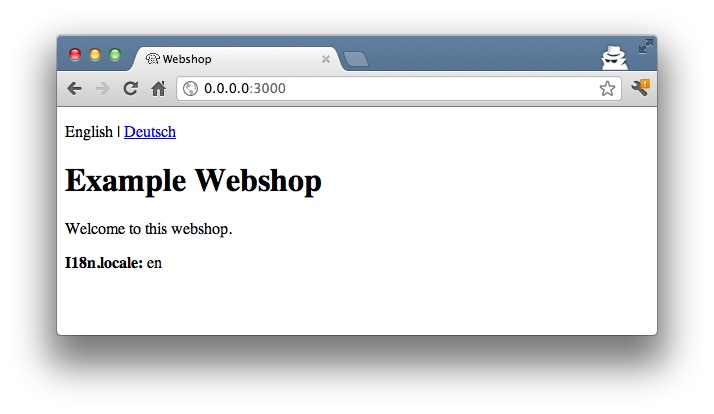
\includegraphics{screenshots/I18n_locale_url_prefix_navigation.jpg}
\end{figure}

\section{Setting I18n.locale via Domain Extension}\label{setting-i18n.locale-via-domain-extension}

If you have several domains with the extensions typical for the corresponding languages, you can of course also use these extensions to set the language. For example, if a user visits the page \url{http://www.example.com}\{.uri\} he would see the English version, if he goes to \url{http://www.example.de}\{.uri\} then the German version would be displayed.

To achieve this, we would need to go into the \texttt{app/controllers/application\_controller.rb} and insert a \texttt{before\_filter} that analyses the accessed domain and sets the \texttt{I18n.locale} :

\begin{shaded}\begin{verbatim}
class ApplicationController < ActionController::Base
  # Prevent CSRF attacks by raising an exception.
  # For APIs, you may want to use :null_session instead.
  protect_from_forgery with: :exception

  before_filter :set_locale

  private
  def set_locale
    case request.host.split('.').last
    when 'de'
      I18n.locale = :de
    when 'com'
      I18n.locale = :en
    else
      I18n.locale = I18n.default_locale
    end
  end
end
\end{verbatim}\end{shaded}

\subsection{Tip}\label{tip-18}

To test this functionality, you can add the following items on your Linux or Mac OS X development system in the file \texttt{/etc/hosts}:

\begin{shaded}\begin{verbatim}
0.0.0.0 www.example.com
0.0.0.0 www.example.de
\end{verbatim}\end{shaded}

Then you can go to the URL \texttt{http://www.example.com:3000} and \texttt{http://www.example.de:3000} and you will see the corresponding language versions.

\section{Which Approach is the Best?}\label{which-approach-is-the-best}

I believe that a combination of the approaches described above will lead to the best result. When I first visit a web page I am happy if I find that the accept language HTTP header of my browser is read and implemented correctly. But it is also nice to be able to change the language later on in the user configuration (in particular for badly translated pages, English language is often better). And ultimately it has to be said that a page that is easy to represent is worth a lot for a search engine, and this also goes for the languages. Rails gives you the option of easily using all variations and even enables you to combine them together.

\chap{Multilingual Scaffolds}\label{multilingual-scaffolds}

As an example, we use a mini webshop in which we translate a product scaffold. The aim is to make the application available in German and English.

The Rails application:

\begin{shaded}\begin{verbatim}
$ rails new webshop
  [...]
$ cd webshop
$ rails generate scaffold Product name description 'price:decimal{7,2}'
  [...]
$ rake db:migrate
  [...]
$
\end{verbatim}\end{shaded}

We define the product model in the \texttt{app/models/product.rb}

\begin{shaded}\begin{verbatim}
class Product < ActiveRecord::Base
  validates :name,
            presence: true,
            uniqueness: true,
            length: { within: 2..255 }

  validates :price,
            presence: true,
            numericality: { greater_than: 0 }
end
\end{verbatim}\end{shaded}

When selecting the language for the user, we use the URL prefix variation described in \hyperref[i18nux5furlux5fpathux5fprefix]{the section called “Setting I18n.locale via URL Path Prefix”}. We use the following \texttt{app/controllers/application\_controller.rb}

\begin{shaded}\begin{verbatim}
class ApplicationController < ActionController::Base
  # Prevent CSRF attacks by raising an exception.
  # For APIs, you may want to use :null_session instead.
  protect_from_forgery with: :exception

  before_filter :set_locale

  def default_url_options
    { locale: I18n.locale }
  end

  private
  def set_locale
    I18n.locale = params[:locale] || I18n.default_locale
  end
end
\end{verbatim}\end{shaded}

This is the \texttt{config/routes.rb}

\begin{shaded}\begin{verbatim}
Webshop::Application.routes.draw do
  scope ':locale', locale: /en|de/ do
    resources :products
    get '/', to: 'products#index'
  end

  root 'products#index'
end
\end{verbatim}\end{shaded}

Then we insert the links for the navigation in the \texttt{app/views/layouts/application.html.erb}:

\begin{shaded}\begin{verbatim}
<!DOCTYPE html>
<html>
<head>
  <title>Webshop</title>
  <%= stylesheet_link_tag    "application", media: "all", "data-turbolinks-track" => true %>
  <%= javascript_include_tag "application", "data-turbolinks-track" => true %>
  <%= csrf_meta_tags %>
</head>
<body>

<p>
<%= link_to_unless I18n.locale == :en, "English", locale: :en %>
|
<%= link_to_unless I18n.locale == :de, "Deutsch", locale: :de %>
</p>

<%= yield %>

</body>
</html>
\end{verbatim}\end{shaded}

Start the Rails server with \textbf{rails server.}

\begin{shaded}\begin{verbatim}
$ rails server
=> Booting WEBrick
=> Rails 4.0.0 application starting in development on http://0.0.0.0:3000
=> Run `rails server -h` for more startup options
=> Ctrl-C to shutdown server
[2013-07-17 22:16:19] INFO  WEBrick 1.3.1
[2013-07-17 22:16:19] INFO  ruby 2.0.0 (2013-06-27) [x86_64-darwin12.4.0]
[2013-07-17 22:16:19] INFO  WEBrick::HTTPServer#start: pid=42806 port=3000
\end{verbatim}\end{shaded}

If we go to \texttt{http://0.0.0.0:3000} we see the normal English page.

\begin{figure}[htbp]
\centering
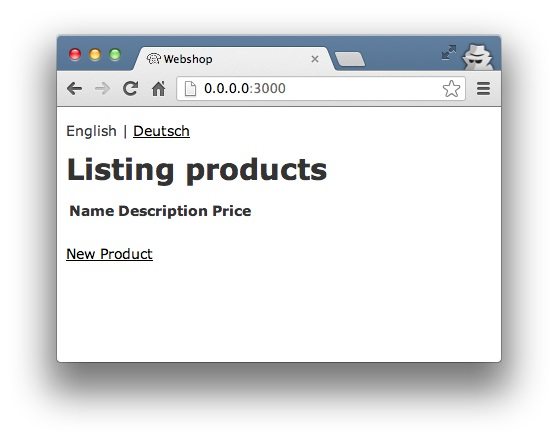
\includegraphics{screenshots/i18n_webshop_base_version.jpg}
\end{figure}

If we click the option German, nothing changes on the page, apart from the language navigation right at the top.

\begin{figure}[htbp]
\centering
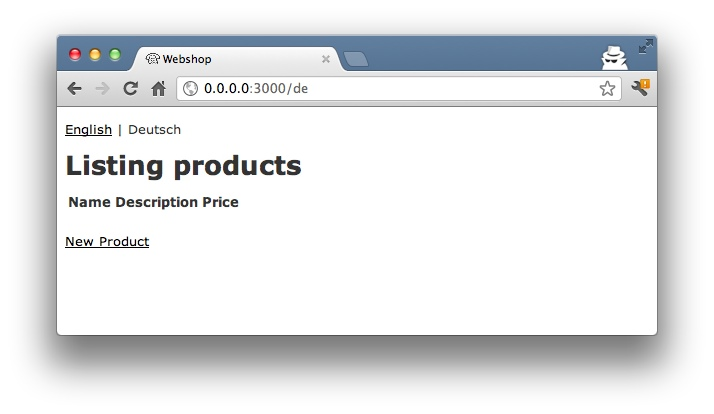
\includegraphics{screenshots/i18n_webshop_base_version_de.jpg}
\end{figure}

Now we still need to find a way of translating the individual elements of this page appropriately and as generically as possible.

\section{Text Blocks in YAML Format}\label{text-blocks-in-yaml-format}

Now we need to define the individual text blocks for \texttt{I18n.t}. The corresponding directories still have to be created first:

\begin{shaded}\begin{verbatim}
$ mkdir -p config/locales/models/product
$ mkdir -p config/locales/views/product
$
\end{verbatim}\end{shaded}

To make sure that the YAML files created there are indeed read in automatically, you need to insert the following lines in the file \texttt{config/application.rb}:

\begin{shaded}\begin{verbatim}
## The default locale is :en and all translations from config/locales/*.rb,yml are auto loaded.
config.i18n.load_path += Dir[Rails.root.join('config', 'locales', 'models', '*', '*.yml').to_s]
config.i18n.load_path += Dir[Rails.root.join('config', 'locales', 'views', '*', '*.yml').to_s]
config.i18n.default_locale = :en
\end{verbatim}\end{shaded}

\section{German}\label{german}

Please create the file \texttt{config/locales/models/product/de.yml} with the following content.

\begin{shaded}\begin{verbatim}
de:
  activerecord:
    models:
      product: 'Produkt'
    attributes:
      product:
        name: 'Name'
        description: 'Beschreibung'
        price: 'Preis'
\end{verbatim}\end{shaded}

In the file \texttt{config/locales/views/product/de.yml} we insert a few values for the scaffold views:

\begin{shaded}\begin{verbatim}
de:
  views:
    show: Anzeigen
    edit: Editieren
    destroy: Löschen
    are_you_sure: Sind Sie sicher?
    back: Zurück
    edit: Editieren
    product:
      index:
        title: Liste aller Produkte
        new_product: Neues Produkt
      edit:
        title: Produkt editieren
      new:
        title: Neues Produkt
      flash_messages:
        product_was_successfully_created: 'Das Produkt wurde erfolgreich angelegt.'
        product_was_successfully_updated: 'Das Produkt wurde erfolgreich aktualisiert.'
\end{verbatim}\end{shaded}

Finally, we copy a ready-made default translation by Sven Fuchs from his github repository \texttt{https://github.com/svenfuchs/rails-i18n}:

\begin{shaded}\begin{verbatim}
$ cd config/locales
$ curl -O https://raw.github.com/svenfuchs/rails-i18n/master/rails/locale/de.yml
  % Total    % Received % Xferd  Average Speed   Time    Time     Time  Current
                                 Dload  Upload   Total   Spent    Left  Speed
100  4940  100  4940    0     0   9574      0 --:--:-- --:--:-- --:--:-- 11932
$ cd ../..
$
\end{verbatim}\end{shaded}

\subsection{Note}\label{note-49}

If you know how Bundler works you can also insert the line \texttt{gem 'rails-i18n'} into the file \texttt{Gemfile} and then execute \textbf{bundle install}. This gives you all language files from the repository.

The file \texttt{config/locales/de.yml} contains all required formats and generic phrases for German that we need for a normal Rails application (for example days of the week, currency symbols, etc). Use your favorite editor to have a look in there to get an impression.

\section{English}\label{english}

As most things are already present in the system for English, we just need to insert a few values for the scaffold views in the file \texttt{config/locales/views/product/en.yml}:

\begin{shaded}\begin{verbatim}
en:
  views:
    show: Show
    edit: Edit
    destroy: Delete
    are_you_sure: Are you sure?
    back: Back
    edit: Edit
    product:
      index:
        title: List of all products
        new_product: New product
      edit:
        title: Edit Product
      new:
        title: New product
      flash_messages:
        product_was_successfully_created: 'Product was successfully created.'
        product_was_successfully_updated: 'Product was successfully updated.'
\end{verbatim}\end{shaded}

\section{Equipping Views with I18n.t}\label{equipping-views-with-i18n.t}

Please edit the listed view files as specified.

\section{\_form.html.erb}\label{form.html.erb}

In the file \texttt{app/views/products/\_form.html.erb} we need to change the display of the validation errors in the top section to \texttt{I18n.t}. The names of form errors are automatically read in from \texttt{activerecord.attributes.product}:

\begin{shaded}\begin{verbatim}
<%= form_for(@product) do |f| %>
  <% if @product.errors.any? %>
    <div id="error_explanation">
      <h2><%= t 'activerecord.errors.template.header', model: Product.model_name.human, count: @product.errors.count %></h2>

      <ul>
      <% @product.errors.full_messages.each do |msg| %>
        <li><%= msg %></li>
      <% end %>
      </ul>
    </div>
  <% end %>

  <div class="field">
    <%= f.label :name %><br>
    <%= f.text_field :name %>
  </div>
  <div class="field">
    <%= f.label :description %><br>
    <%= f.text_field :description %>
  </div>
  <div class="field">
    <%= f.label :price %><br>
    <%= f.text_field :price %>
  </div>
  <div class="actions">
    <%= f.submit %>
  </div>
<% end %>
\end{verbatim}\end{shaded}

\section{edit.html.erb}\label{edit.html.erb}

In the file \texttt{app/views/products/edit.html.erb} we need to integrate the heading and the links at the bottom of the page with \texttt{I18n.t}:

\begin{shaded}\begin{verbatim}
<h1><%= t 'views.product.edit.title' %></h1>

<%= render 'form' %>

<%= link_to I18n.t('views.show'), @product %> |
<%= link_to I18n.t('views.back'), products_path %>
\end{verbatim}\end{shaded}

\section{index.html.erb}\label{index.html.erb}

In the file \texttt{app/views/products/index.html.erb} we need to change practically every line. In the table header I use \texttt{human\_attribute\_name()}, but you could also do it directly with \texttt{I18n.t}. The price of the product is specified with the helper number\_to\_currency. In a real application, we would have to specify a defined currency at this point as well.

\begin{shaded}\begin{verbatim}
<h1><%= t 'views.product.index.listing_products' %></h1>

<table>
  <thead>
    <tr>
      <th><%= Product.human_attribute_name(:name) %></th>
      <th><%= Product.human_attribute_name(:description) %></th>
      <th><%= Product.human_attribute_name(:price) %></th>
      <th></th>
      <th></th>
      <th></th>
    </tr>
  </thead>

  <tbody>
    <% @products.each do |product| %>
      <tr>
        <td><%= product.name %></td>
        <td><%= product.description %></td>
        <td><%= number_to_currency(product.price) %></td>
        <td><%= link_to I18n.t('views.show'), product %></td>
        <td><%= link_to I18n.t('views.edit'), edit_product_path(product) %></td>
        <td><%= link_to I18n.t('views.destroy'), product, method: :delete, data: { confirm: I18n.t('views.are_you_sure')} %></td>
      </tr>
    <% end %>
  </tbody>
</table>

<br>

<%= link_to I18n.t('views.product.index.new_product'), new_product_path %>
\end{verbatim}\end{shaded}

\section{new.html.erb}\label{new.html.erb}

In the \texttt{app/views/products/new.html.erb} we need to adapt the heading and the link:

\begin{shaded}\begin{verbatim}
<h1><%= t 'views.product.new.title' %></h1>

<%= render 'form' %>

<%= link_to I18n.t('views.back'), products_path %>
\end{verbatim}\end{shaded}

\section{show.html.erb}\label{show.html.erb}

In the \texttt{app/views/products/show.html.erb} we again use \texttt{human\_attribute\_name()} for the attributes. Plus the links need to be translated with \texttt{I18n.t}. As with the index view, we again use \texttt{number\_to\_currency()} to show the price in formatted form:

\begin{shaded}\begin{verbatim}
<p id="notice"><%= notice %></p>

<p>
  <strong><%= Product.human_attribute_name(:name) %>:</strong>
  <%= @product.name %>
</p>

<p>
  <strong><%= Product.human_attribute_name(:description) %>:</strong>
  <%= @product.description %>
</p>

<p>
  <strong><%= Product.human_attribute_name(:price) %>:</strong>
  <%= number_to_currency(@product.price) %>
</p>

<%= link_to I18n.t('views.edit'), edit_product_path(@product) %> |
<%= link_to I18n.t('views.back'), products_path %>
\end{verbatim}\end{shaded}

\section{Translating Flash Messages in the Controller}\label{translating-flash-messages-in-the-controller}

Finally, we need to translate the two flash messages in the \texttt{app/controllers/products\_controller.rb} for creating (create) and updating (update) records, again via \texttt{I18n.t}:

\begin{shaded}\begin{verbatim}
class ProductsController < ApplicationController
  before_action :set_product, only: [:show, :edit, :update, :destroy]

  # GET /products
  # GET /products.json
  def index
    @products = Product.all
  end

  # GET /products/1
  # GET /products/1.json
  def show
  end

  # GET /products/new
  def new
    @product = Product.new
  end

  # GET /products/1/edit
  def edit
  end

  # POST /products
  # POST /products.json
  def create
    @product = Product.new(product_params)

    respond_to do |format|
      if @product.save
        format.html { redirect_to @product, notice: I18n.t('views.product.flash_messages.product_was_successfully_created') }
        format.json { render action: 'show', status: :created, location: @product }
      else
        format.html { render action: 'new' }
        format.json { render json: @product.errors, status: :unprocessable_entity }
      end
    end
  end

  # PATCH/PUT /products/1
  # PATCH/PUT /products/1.json
  def update
    respond_to do |format|
      if @product.update(product_params)
        format.html { redirect_to @product, notice: I18n.t('views.product.flash_messages.product_was_successfully_updated') }
        format.json { head :no_content }
      else
        format.html { render action: 'edit' }
        format.json { render json: @product.errors, status: :unprocessable_entity }
      end
    end
  end

  # DELETE /products/1
  # DELETE /products/1.json
  def destroy
    @product.destroy
    respond_to do |format|
      format.html { redirect_to products_url }
      format.json { head :no_content }
    end
  end

  private
    # Use callbacks to share common setup or constraints between actions.
    def set_product
      @product = Product.find(params[:id])
    end

    # Never trust parameters from the scary internet, only allow the white list through.
    def product_params
      params.require(:product).permit(:name, :description, :price)
    end
end
\end{verbatim}\end{shaded}

\section{The Result}\label{the-result}

Now you can use the scaffold products both in German and in English. You can switch the language via the link at the top of the page.

\section{Further Information}\label{further-information-1}

The best source of information on this topic can be found in the Rails documentation at \url{http://guides.rubyonrails.org/i18n.html}\{.uri\}. This also shows how you can operate other backends for defining the translations.

As so often, \texttt{Railscasts.com} offers a whole range of Railscasts on the topic I18n: \texttt{http://railscasts.com/episodes?utf8=\%E2\%9C\%93\&search=i18n}

\chap{Bundler and Gems}\label{bundler-and-gems}

\hyperdef{}{gems}{\section{Gems}\label{gems}}

Gems constitute the package management in the world of Ruby. If a Ruby developer wants to offer a specific feature or a certain program or collection of programs to other Ruby developers, he can create a “gem” from these. This gem can then be installed via \textbf{gem install}. How to create a gem and where it can be hosted goes beyond the scope of this introduction chapter. The important thing for our purposes is that for example Rails in itself is also available as gem.

\chap{Bundler}\label{bundler}

In a Rails project, different gems are used (see \hyperref[gems]{the section called “Gems”}) and a developer can also add further gems. Bundler helps the developer to install all these gems in the right version and to take into account important dependencies. In previous Rails versions, you as developer had to always call a \textbf{bundle install} after a \textbf{rails new}. Now, this is done automatically within \textbf{rails new}. In the output you can see which gems are installed by \textbf{bundle install}:

\begin{shaded}\begin{verbatim}
$ rails new webshop
  [...]
       run  bundle install
Fetching gem metadata from https://rubygems.org/..........
Fetching gem metadata from https://rubygems.org/..
Resolving dependencies...
Using rake (10.1.0)
Using i18n (0.6.4)
Using minitest (4.7.5)
Using multi_json (1.7.7)
Using atomic (1.1.10)
Using thread_safe (0.1.0)
Using tzinfo (0.3.37)
Using activesupport (4.0.0)
Using builder (3.1.4)
Using erubis (2.7.0)
Using rack (1.5.2)
Using rack-test (0.6.2)
Using actionpack (4.0.0)
Using mime-types (1.23)
Using polyglot (0.3.3)
Using treetop (1.4.14)
Using mail (2.5.4)
Using actionmailer (4.0.0)
Using activemodel (4.0.0)
Using activerecord-deprecated_finders (1.0.3)
Using arel (4.0.0)
Using activerecord (4.0.0)
Using bundler (1.3.5)
Using coffee-script-source (1.6.3)
Using execjs (1.4.0)
Using coffee-script (2.2.0)
Using thor (0.18.1)
Using railties (4.0.0)
Using coffee-rails (4.0.0)
Using hike (1.2.3)
Using jbuilder (1.4.2)
Using jquery-rails (3.0.4)
Using json (1.8.0)
Using tilt (1.4.1)
Using sprockets (2.10.0)
Using sprockets-rails (2.0.0)
Using rails (4.0.0)
Using rdoc (3.12.2)
Using sass (3.2.9)
Using sass-rails (4.0.0)
Using sdoc (0.3.20)
Using sqlite3 (1.3.7)
Using turbolinks (1.3.0)
Using uglifier (2.1.2)
Your bundle is complete!
Use `bundle show [gemname]` to see where a bundled gem is installed.
$ cd webshop
$
\end{verbatim}\end{shaded}

The file \texttt{Gemfile} generated by \textbf{rails new} indicates which gems are to be installed by Bundler:

\begin{shaded}\begin{verbatim}
source 'https://rubygems.org'

## Bundle edge Rails instead: gem 'rails', github: 'rails/rails'
gem 'rails', '4.0.0'

## Use sqlite3 as the database for Active Record
gem 'sqlite3'

## Use SCSS for stylesheets
gem 'sass-rails', '~> 4.0.0'

## Use Uglifier as compressor for JavaScript assets
gem 'uglifier', '>= 1.3.0'

## Use CoffeeScript for .js.coffee assets and views
gem 'coffee-rails', '~> 4.0.0'

## See https://github.com/sstephenson/execjs#readme for more supported runtimes
## gem 'therubyracer', platforms: :ruby

## Use jquery as the JavaScript library
gem 'jquery-rails'

## Turbolinks makes following links in your web application faster. Read more: https://github.com/rails/turbolinks
gem 'turbolinks'

## Build JSON APIs with ease. Read more: https://github.com/rails/jbuilder
gem 'jbuilder', '~> 1.2'

group :doc do
  # bundle exec rake doc:rails generates the API under doc/api.
  gem 'sdoc', require: false
end

## Use ActiveModel has_secure_password
## gem 'bcrypt-ruby', '~> 3.0.0'

## Use unicorn as the app server
## gem 'unicorn'

## Use Capistrano for deployment
## gem 'capistrano', group: :development

## Use debugger
## gem 'debugger', group: [:development, :test]
\end{verbatim}\end{shaded}

The format used is easy to explain: the word \texttt{gem} is followed by the name of the gem and then, if required, a specification of the version of the gem.

For example, the line \texttt{gem 'rails', '4.0.0'} stands for “install the gem with the name \texttt{rails} in the version 4.0.0”.

With \texttt{\textasciitilde{}\textgreater{}} before the version number you can determine that the newest version after this version number should be installed. As a result, the last digit is incremented, so for example \texttt{gem 'rails',     '\textasciitilde{}\textgreater{} 4.0.0'} would correspondingly install a Rails 4.0.1, but not a 4.1 (for the latter, you would need to specify \texttt{gem 'rails', '\textasciitilde{}\textgreater{}     4.0'}).

\subsection{Important}\label{important-13}

You have the option of installing certain gems only in certain environments. To do so, you need to enclose the corresponding lines in a \texttt{group :name do} loop.

Apart from the file \texttt{Gemfile} there is also the file \texttt{Gemfile.lock} and the exact versions of the installed gems are listed there. In the above example, it looks like this:

\begin{shaded}\begin{verbatim}
GEM
  remote: https://rubygems.org/
  specs:
    actionmailer (4.0.0)
      actionpack (= 4.0.0)
      mail (~> 2.5.3)
    actionpack (4.0.0)
      activesupport (= 4.0.0)
      builder (~> 3.1.0)
      erubis (~> 2.7.0)
      rack (~> 1.5.2)
      rack-test (~> 0.6.2)
    activemodel (4.0.0)
      activesupport (= 4.0.0)
      builder (~> 3.1.0)
    activerecord (4.0.0)
      activemodel (= 4.0.0)
      activerecord-deprecated_finders (~> 1.0.2)
      activesupport (= 4.0.0)
      arel (~> 4.0.0)
    activerecord-deprecated_finders (1.0.3)
    activesupport (4.0.0)
      i18n (~> 0.6, >= 0.6.4)
      minitest (~> 4.2)
      multi_json (~> 1.3)
      thread_safe (~> 0.1)
      tzinfo (~> 0.3.37)
    arel (4.0.0)
    atomic (1.1.10)
    builder (3.1.4)
    coffee-rails (4.0.0)
      coffee-script (>= 2.2.0)
      railties (>= 4.0.0.beta, < 5.0)
    coffee-script (2.2.0)
      coffee-script-source
      execjs
    coffee-script-source (1.6.3)
    erubis (2.7.0)
    execjs (1.4.0)
      multi_json (~> 1.0)
    hike (1.2.3)
    i18n (0.6.4)
    jbuilder (1.4.2)
      activesupport (>= 3.0.0)
      multi_json (>= 1.2.0)
    jquery-rails (3.0.4)
      railties (>= 3.0, < 5.0)
      thor (>= 0.14, < 2.0)
    json (1.8.0)
    mail (2.5.4)
      mime-types (~> 1.16)
      treetop (~> 1.4.8)
    mime-types (1.23)
    minitest (4.7.5)
    multi_json (1.7.7)
    polyglot (0.3.3)
    rack (1.5.2)
    rack-test (0.6.2)
      rack (>= 1.0)
    rails (4.0.0)
      actionmailer (= 4.0.0)
      actionpack (= 4.0.0)
      activerecord (= 4.0.0)
      activesupport (= 4.0.0)
      bundler (>= 1.3.0, < 2.0)
      railties (= 4.0.0)
      sprockets-rails (~> 2.0.0)
    railties (4.0.0)
      actionpack (= 4.0.0)
      activesupport (= 4.0.0)
      rake (>= 0.8.7)
      thor (>= 0.18.1, < 2.0)
    rake (10.1.0)
    rdoc (3.12.2)
      json (~> 1.4)
    sass (3.2.9)
    sass-rails (4.0.0)
      railties (>= 4.0.0.beta, < 5.0)
      sass (>= 3.1.10)
      sprockets-rails (~> 2.0.0)
    sdoc (0.3.20)
      json (>= 1.1.3)
      rdoc (~> 3.10)
    sprockets (2.10.0)
      hike (~> 1.2)
      multi_json (~> 1.0)
      rack (~> 1.0)
      tilt (~> 1.1, != 1.3.0)
    sprockets-rails (2.0.0)
      actionpack (>= 3.0)
      activesupport (>= 3.0)
      sprockets (~> 2.8)
    sqlite3 (1.3.7)
    thor (0.18.1)
    thread_safe (0.1.0)
      atomic
    tilt (1.4.1)
    treetop (1.4.14)
      polyglot
      polyglot (>= 0.3.1)
    turbolinks (1.3.0)
      coffee-rails
    tzinfo (0.3.37)
    uglifier (2.1.2)
      execjs (>= 0.3.0)
      multi_json (~> 1.0, >= 1.0.2)

PLATFORMS
  ruby

DEPENDENCIES
  coffee-rails (~> 4.0.0)
  jbuilder (~> 1.2)
  jquery-rails
  rails (= 4.0.0)
  sass-rails (~> 4.0.0)
  sdoc
  sqlite3
  turbolinks
  uglifier (>= 1.3.0)
\end{verbatim}\end{shaded}

The advantage of \texttt{Gemfile.lock} is that it makes it possible for several developers to work on the same Rails project independently from one another and to still be sure that they are all working with the same gem versions. If a file is \texttt{Gemfile.lock}, this will be used by the Bundler. This is also useful for deploying the Rails project later on a web server.

Thanks to this mechanism you can use and develop several Rails projects with different gem version numbers in parallel.

\section{bundle update}\label{bundle-update}

With \textbf{bundle update} you can update gems to new versions. As an example, I have a Rails project with the Rails version 4.0.0:

\begin{shaded}\begin{verbatim}
$ rails -v
Rails 4.0.0
$
\end{verbatim}\end{shaded}

In the file \texttt{Gemfile}, this version is listed:

\begin{shaded}\begin{verbatim}
$ head -n 4 Gemfile
source 'https://rubygems.org'

## Bundle edge Rails instead: gem 'rails', github: 'rails/rails'
gem 'rails', '4.0.0'
$
\end{verbatim}\end{shaded}

And also in the \texttt{Gemfile.lock}:

\begin{shaded}\begin{verbatim}
$ grep 'rails' Gemfile.lock
    coffee-rails (4.0.0)
    jquery-rails (3.0.4)
    rails (4.0.0)
      sprockets-rails (~> 2.0.0)
    sass-rails (4.0.0)
      sprockets-rails (~> 2.0.0)
    sprockets-rails (2.0.0)
      coffee-rails
  coffee-rails (~> 4.0.0)
  jquery-rails
  rails (= 4.0.0)
  sass-rails (~> 4.0.0)
$
\end{verbatim}\end{shaded}

If we want to update this Rails project to the Rails version 4.0.1, we need to change the entry in the \texttt{Gemfile} as follows:

\begin{shaded}\begin{verbatim}
source 'https://rubygems.org'

## Bundle edge Rails instead: gem 'rails', github: 'rails/rails'
gem 'rails', '4.0.1'

## Use sqlite3 as the database for Active Record
gem 'sqlite3'

## Use SCSS for stylesheets
gem 'sass-rails', '~> 4.0.0'

## Use Uglifier as compressor for JavaScript assets
gem 'uglifier', '>= 1.3.0'

## Use CoffeeScript for .js.coffee assets and views
gem 'coffee-rails', '~> 4.0.0'

# See https://github.com/sstephenson/execjs#readme for more supported runtimes
## gem 'therubyracer', platforms: :ruby

## Use jquery as the JavaScript library
gem 'jquery-rails'

## Turbolinks makes following links in your web application faster. Read more: https://github.com/rails/turbolinks
gem 'turbolinks'

## Build JSON APIs with ease. Read more: https://github.com/rails/jbuilder
gem 'jbuilder', '~> 1.2'

group :doc do
  # bundle exec rake doc:rails generates the API under doc/api.
  gem 'sdoc', require: false
end

## Use ActiveModel has_secure_password
## gem 'bcrypt-ruby', '~> 3.0.0'

## Use unicorn as the app server
## gem 'unicorn'

## Use Capistrano for deployment
## gem 'capistrano', group: :development

## Use debugger
## gem 'debugger', group: [:development, :test]
\end{verbatim}\end{shaded}

After this change, you can use \textbf{bundle update rails} to install the new Rails version (required dependencies are automatically taken into account by Bundler):

\begin{shaded}\begin{verbatim}
$ bundle update rails
  [...]
$ rails -v
Rails 4.0.1
$
\end{verbatim}\end{shaded}

\subsection{Important}\label{important-14}

After every gem update, you should first run \textbf{rake test} to make sure that a new gem version does not add any unwanted side effects.

\section{bundle outdated}\label{bundle-outdated}

If you want to know which of the gems used by your Rails project are now available in a new version, you can do this via the command \textbf{bundle outdated}. Example:

\begin{shaded}\begin{verbatim}
$ bundle outdated
Fetching gem metadata from https://rubygems.org/..........
Fetching gem metadata from https://rubygems.org/..
Resolving dependencies...

Outdated gems included in the bundle:
  * builder (3.2.2 > 3.1.4)
  * minitest (5.0.6 > 4.7.5)
  * rdoc (4.0.1 > 3.12.2)
  * tzinfo (1.0.1 > 0.3.37)
$
\end{verbatim}\end{shaded}

\section{bundle exec}\label{bundle-exec}

\textbf{bundle exec} is probably one of the commands Rails developers hate the most. It is required whenever a program such as \textbf{rake} is used in a Rails project and is present in a different version than the rest of the system. The resulting error message is always easy to implement:

\begin{shaded}\begin{verbatim}
You have already activated rake 0.10, but your Gemfile requires rake 0.9.2.2. Using bundle exec may solve this.
\end{verbatim}\end{shaded}

In this case, it helps to invoke the command with a preceding \textbf{bundle exec}:

\begin{shaded}\begin{verbatim}
$ bundle exec rake db:migrate
\end{verbatim}\end{shaded}

\section{binstubs}\label{binstubs}

In some environments, using \textbf{bundle exec} is too complicated. In that case, you can install programs with the correct version via \textbf{bundle install --binstubs} in the directory bin:

\begin{shaded}\begin{verbatim}
$ bundle install --binstubs
Using rake (10.1.0)
Using i18n (0.6.4)
Using minitest (4.7.5)
Using multi_json (1.7.7)
Using atomic (1.1.10)
Using thread_safe (0.1.0)
Using tzinfo (0.3.37)
Using activesupport (4.0.0)
Using builder (3.1.4)
Using erubis (2.7.0)
Using rack (1.5.2)
Using rack-test (0.6.2)
Using actionpack (4.0.0)
Using mime-types (1.23)
Using polyglot (0.3.3)
Using treetop (1.4.14)
Using mail (2.5.4)
Using actionmailer (4.0.0)
Using activemodel (4.0.0)
Using activerecord-deprecated_finders (1.0.3)
Using arel (4.0.0)
Using activerecord (4.0.0)
Using coffee-script-source (1.6.3)
Using execjs (1.4.0)
Using coffee-script (2.2.0)
Using thor (0.18.1)
Using railties (4.0.0)
Using coffee-rails (4.0.0)
Using hike (1.2.3)
Using jbuilder (1.4.2)
Using jquery-rails (3.0.4)
Using json (1.8.0)
Using bundler (1.3.5)
Using tilt (1.4.1)
Using sprockets (2.10.0)
Using sprockets-rails (2.0.0)
Using rails (4.0.0)
Using rdoc (3.12.2)
Using sass (3.2.9)
Using sass-rails (4.0.0)
Using sdoc (0.3.20)
Using sqlite3 (1.3.7)
Using turbolinks (1.3.0)
Using uglifier (2.1.2)
Your bundle is complete!
Use `bundle show [gemname]` to see where a bundled gem is installed.
SW:webshop stefan$ ls bin
bundle  rake  sass-convert  sprockets
erubis  rdoc  scss          thor
rackup  ri    sdoc          tilt
rails   sass  sdoc-merge    tt
$
\end{verbatim}\end{shaded}

Afterwards, you can always use these programs. Example:

\begin{shaded}\begin{verbatim}
$ bin/rake db:migrate
==  CreateUsers: migrating ====================================================
-- create_table(:users)
   -> 0.0018s
==  CreateUsers: migrated (0.0019s) ===========================================

$
\end{verbatim}\end{shaded}

\chap{Further Information on Bundler}\label{further-information-on-bundler}

The topic Bundler is far more complex than can be described here. If you want to find out more on Bundler, please visit the following websites to find further information:

\begin{itemize}
\itemsep1pt\parskip0pt\parsep0pt
\item
  \url{http://railscasts.com/episodes/201-bundler-revised}
\item
  \url{http://gembundler.com/}
\end{itemize}

\chap{Asset Pipeline}\label{asset-pipeline}

\section{Introduction}\label{introduction-5}

The asset pipeline offers the Rails developer the opportunity of delivering CSS, JavaScript and image files to the browser more optimally - in other words, in a more compressed form and therefore more quickly. Different CSS files are combined into one big file and delivered to the browser with a fingerprint in the file name. This fingerprinting enables the browser and any proxy in between to optimally cache the data, so the browser can load these files more quickly.

Within the asset pipeline, you can program CSS, SASS, JavaScript and CoffeeScript extensively and clearly, in order to let them be delivered later as automatically compressed CSS and JavaScript files.

As an example we use once more our web shop with a product scaffold:

\begin{shaded}\begin{verbatim}
$ rails new webshop
  [...]
$ cd webshop
$ rails generate scaffold product name 'price:decimal{7,2}'
  [...]
$ rake db:migrate
  [...]
$
\end{verbatim}\end{shaded}

In the directory \texttt{app/assets} you will then find the following files:

\begin{shaded}\begin{verbatim}
app/assets
├── images
├── javascripts
│   ├── application.js
│   └── products.js.coffee
└── stylesheets
    ├── application.css
    ├── products.css.scss
    └── scaffolds.css.scss
\end{verbatim}\end{shaded}

The files \texttt{app/assets/javascripts/application.js} and \texttt{app/assets/stylesheets/application.css} are what is referred to as manifest files. They automatically include the other files in the relevant directory.

\section{Manifest Files}\label{manifest-files}

In \texttt{app/assets/javascripts} and \texttt{app/assets/stylesheets} there are always manifest files that contain instructions to the asset pipeline. They define everything that is to be integrated.

\section{application.js}\label{application.js}

The file \texttt{app/assets/javascripts/application.js} has the following content:

\begin{shaded}\begin{verbatim}
// This is a manifest file that'll be compiled into application.js, which will include all the files
// listed below.
//
// Any JavaScript/Coffee file within this directory, lib/assets/javascripts, vendor/assets/javascripts,
// or vendor/assets/javascripts of plugins, if any, can be referenced here using a relative path.
//
// It's not advisable to add code directly here, but if you do, it'll appear at the bottom of the
// compiled file.
//
// Read Sprockets README (https://github.com/sstephenson/sprockets#sprockets-directives) for details
// about supported directives.
//
//= require jquery
//= require jquery_ujs
//= require turbolinks
//= require_tree .
\end{verbatim}\end{shaded}

In the \texttt{application.js}, the jQuery files defined in the \texttt{jquery-rails} gem are automatically integrated (for further information on jQuery, please visit \url{http://jquery.com/}\{.uri\}). Plus all other files in this directory are integrated via \texttt{require\_tree         .} as shown above.

The not yet optimized result can be viewed in the development environment at the URL \texttt{http://0.0.0.0:3000/assets/application.js}.

\section{application.css}\label{application.css}

The file \texttt{app/assets/stylesheets/application.css} has the following content:

\begin{shaded}\begin{verbatim}
/*
 * This is a manifest file that'll be compiled into application.css, which will include all the files
 * listed below.
 *
 * Any CSS and SCSS file within this directory, lib/assets/stylesheets, vendor/assets/stylesheets,
 * or vendor/assets/stylesheets of plugins, if any, can be referenced here using a relative path.
 *
 * You're free to add application-wide styles to this file and they'll appear at the top of the
 * compiled file, but it's generally better to create a new file per style scope.
 *
 *= require_self
 *= require_tree .
 */
\end{verbatim}\end{shaded}

With the command \texttt{require\_tree .} all files in this directory are automatically integrated.

\section{rake assets:precompile}\label{rake-assetsprecompile}

When using the asset pipeline, you need to remember that you have to precompile the assets before starting the Rails server in the production environment. This happens via the command \textbf{rake assets:precompile:}

\begin{shaded}\begin{verbatim}
$ rake assets:precompile
I, [2013-07-17T22:58:32.807148 #42981]  INFO -- : Writing /Users/xyz/webshop/public/assets/application-723d1be6cc741a3aabb1cec24276d681.js
I, [2013-07-17T22:58:32.880512 #42981]  INFO -- : Writing /Users/xyz/webshop/public/assets/application-12b3c7dd74d2e9df37e7cbb1efa76a6d.css
$
\end{verbatim}\end{shaded}

\subsection{Note}\label{note-50}

If you forget to do this, you will find the following error message in the log:

\begin{shaded}\begin{verbatim}
ActionView::Template::Error (application.css isn't precompiled)
\end{verbatim}\end{shaded}

The files created by \textbf{rake assets:precompile} appear in the directory \texttt{public/assets}

\begin{shaded}\begin{verbatim}
public/assets/
├── application-12b3c7dd74d2e9df37e7cbb1efa76a6d.css
├── application-12b3c7dd74d2e9df37e7cbb1efa76a6d.css.gz
├── application-723d1be6cc741a3aabb1cec24276d681.js
├── application-723d1be6cc741a3aabb1cec24276d681.js.gz
└── manifest-720d2116dee3d83d194ffd9d0957c21c.json
\end{verbatim}\end{shaded}

Go ahead and use your favorite editor to have a look at the created \texttt{css} and \texttt{js} files. You will find optimized code. If the web server supports it, the zipped \texttt{gz} files are delivered directly, which speeds things up a bit more.

\subsection{Note}\label{note-51}

The difference in file size is enormous. The file \texttt{application.js} created in the development environment has a file size of 296 KB. The file \texttt{js.gz} created by \textbf{rake assets:precompile} is only 88 KB. Users of cellphones in particular will be grateful for smaller file sizes.

The speed advantage incidentally lies not just in the file size, but also in the fact that only one file is downloaded, not several. The HTTP overhead for loading a file is time-consuming.

\section{The Fingerprint}\label{the-fingerprint}

The fingerprint in the file name consists of a hash sum generated from the content of the relevant file. This fingerprint ensures optimal caching and prevents an old cache being used if any changes are made to the content. A simple but very effective method.

\section{Coding Links to an Asset}\label{coding-links-to-an-asset}

All files below the directory \texttt{app/assets} are delivered in normal form by the Rails server. For example, you can go to the URL \texttt{http://0.0.0.0:3000/assets/rails.png} to view the Rails logo saved under \texttt{app/assets/images/rails.png} and to \texttt{http://0.0.0.0:3000/assets/application.js} to view the content of \texttt{app/assets/javascripts/application.js}. The Rails image \texttt{rails.png} is delivered 1:1 and the file \texttt{application.js} is first created by the asset pipeline.

But you should never enter these files as hard-wired in a view. To make the most of the asset pipeline, you must use the helpers described here.

\section{Coding Link to an Image}\label{coding-link-to-an-image}

You can retrieve an image via the helper \texttt{image\_tag}. This is what it would look like in the view for the file \texttt{app/assets/images/rails.png}:

\begin{shaded}\begin{verbatim}
<%= image_tag "rails.png" %>
\end{verbatim}\end{shaded}

In development mode, the following HTML code results from this:

\begin{shaded}\begin{verbatim}
<img alt="Rails" src="/assets/rails.png" />
\end{verbatim}\end{shaded}

In production mode, you get an HTML code that points to a precompiled file with fingerprint:

\begin{shaded}\begin{verbatim}
<img alt="Rails" src="/assets/rails-be8732dac73d845ac5b142c8fb5f9fb0.png" />
\end{verbatim}\end{shaded}

\section{Coding Link to a JavaScript File}\label{coding-link-to-a-javascript-file}

You can use the helper \texttt{javascript\_include\_tag} to retrieve a JavaScript file compiled by the asset pipeline. This is what it would look like in the view for the file \texttt{app/assets/javascripts/application.js}:

\begin{shaded}\begin{verbatim}
%= javascript_include_tag "application" %>
\end{verbatim}\end{shaded}

In development mode, the following HTML code results from this:

\begin{shaded}\begin{verbatim}
<link href="/assets/application.css?body=1" media="all" rel="stylesheet" type="text/css" />
<link href="/assets/products.css?body=1" media="all" rel="stylesheet" type="text/css" />
<link href="/assets/scaffolds.css?body=1" media="all" rel="stylesheet" type="text/css" />
\end{verbatim}\end{shaded}

In production mode, you get an HTML code that points to a precompiled file with fingerprint:

\begin{shaded}\begin{verbatim}
<link href="/assets/application-0149f820dbdd285aa65e241569d8c256.css" media="all" rel="stylesheet" type="text/css" />
\end{verbatim}\end{shaded}

\section{Coding Link to a CSS File}\label{coding-link-to-a-css-file}

A stylesheet compiled by the asset pipeline can be retrieved via the helper \texttt{stylesheet\_link\_tag}. In the view, it would look like this for the file \texttt{app/assets/stylesheets/application.css}:

\begin{shaded}\begin{verbatim}
<%= stylesheet_link_tag "application" %>
\end{verbatim}\end{shaded}

In development mode, the following HTML code results from this:

\begin{shaded}\begin{verbatim}
<script src="/assets/jquery.js?body=1" type="text/javascript"></script>
<script src="/assets/jquery_ujs.js?body=1" type="text/javascript"></script>
<script src="/assets/products.js?body=1" type="text/javascript"></script>
<script src="/assets/application.js?body=1" type="text/javascript"></script>
\end{verbatim}\end{shaded}

In production mode, you get an HTML code that points to a precompiled file with fingerprint:

\begin{shaded}\begin{verbatim}
<script src="/assets/application-f8ca698e63b86d217c88772a65d2d20e.js" type="text/javascript"></script>
\end{verbatim}\end{shaded}

\section{Defaults in the application.html.erb}\label{defaults-in-the-application.html.erb}

Incidentally, the file \texttt{app/views/layouts/application.html.erb} that the scaffold generator creates by default already contains the coding links for these JavaScript and stylesheet files:

\begin{shaded}\begin{verbatim}
<!DOCTYPE html>
<html>
<head>
  <title>Webshop</title>
  <%= stylesheet_link_tag    "application", media: "all", "data-turbolinks-track" => true %>
  <%= javascript_include_tag "application", "data-turbolinks-track" => true %>
  <%= csrf_meta_tags %>
</head>
<body>

<%= yield %>

</body>
</html>
\end{verbatim}\end{shaded}

\chap{JavaScript}\label{javascript}

\section{Introduction}\label{introduction-6}

The focus of this chapter is not on explaining JavaScript. The aim is to show you as a Rails programmer how you can integrate JavaScript in a Rails application. Correspondingly, the chapters do not explain JavaScript in detail. I am assuming that you can read and understand JavaScript. If not, it may be better to skip this chapter. You can happily get by without JavaScript.

\chap{jQuery}\label{jquery}

By default, Rails 4 uses the jQuery Javascript library (\url{http://jquery.com/}\{.uri\}). If you do not require this library, you should delete the following items from the file \texttt{app/assets/javascripts/application.js} within the asset pipeline (see \hyperref[assetux5fpipeline]{Chapter~12, \emph{Asset Pipeline}}):

\begin{shaded}\begin{verbatim}
//= require jquery
//= require jquery_ujs
\end{verbatim}\end{shaded}

With jQuery, you can implement animations and Ajax interactions on your web page relatively easily.

You will find a good introduction to this topic in the jQuery documentation at \url{http://learn.jquery.com/}\{.uri\}

\section{CoffeeScript}\label{coffeescript}

For many Rails developers, CoffeeScript is the best thing invented since the introduction of sliced bread. CoffeeScript is a simple programming language that is converted to JavaScript via the asset pipeline. I am going to use JavaScript and CoffeeScript in this chapter. If you would like to know more about CoffeeScript, please look at the CoffeeScript documentation at \url{http://coffeescript.org/}\{.uri\} and as so often there is also an excellent Railscast on CoffeeScript available at \url{http://railscasts.com/episodes/267-coffeescript-basics.}\{.uri\}

\section{JavaScript Helpers}\label{javascript-helpers}

For using JavaScript in the view, there are some useful helpers available.

\section{javascript\_tag}\label{javascriptux5ftag}

The easiest way of using JavaScript in a view is via\texttt{javascript\_tag}.

With the following line in the view, you can execute an alert when the page is accessed:

\begin{shaded}\begin{verbatim}
<%= javascript_tag "alert('Just an example.')" %>
\end{verbatim}\end{shaded}

The HTML code generated is this:

\begin{shaded}\begin{verbatim}
<script type="text/javascript">
//<![CDATA[
alert('Just an example.')
//]]>
</script>
\end{verbatim}\end{shaded}

\section{link\_to\_function}\label{linkux5ftoux5ffunction}

The helper \texttt{link\_to\_function} creates a link whose \texttt{onclick} handler executes a JavaScript.

Again, here is a example for an alert. The ERB code in the view looks like this:

\begin{shaded}\begin{verbatim}
<%= link_to_function "trigger alert", "alert('Just an example.')" %>
\end{verbatim}\end{shaded}

The generated HTML code:

\begin{shaded}\begin{verbatim}
<a href="#" onclick="alert('Just an example.'); return false;">trigger alert</a>
\end{verbatim}\end{shaded}

\section{button\_to\_function}\label{buttonux5ftoux5ffunction}

The helper \texttt{button\_to\_function} creates a button whose \texttt{onclick} handler executes a JavaScript.

Once more the example with the alert. The ERB code in the view looks like this:

\begin{shaded}\begin{verbatim}
<%= button_to_function "trigger alert", "alert('Just an example.')" %>
\end{verbatim}\end{shaded}

The generated HTML code:

\begin{shaded}\begin{verbatim}
<input onclick="alert('Just an example.');" type="button" value="trigger alert" />
\end{verbatim}\end{shaded}

\section{Example}\label{example}

The easiest way of explaining how you go about programming with JavaScript and the asset pipeline in a Rails project is by using a little example. As always, the main focus is not on creating an amazingly meaningful application. ;-)

\chap{Changing Form Depending on Input}\label{changing-form-depending-on-input}

Let's build a room reservation where you can book a single or double room and then have to enter either one or two guest names in the same form. The basic structure:

\begin{shaded}\begin{verbatim}
$ rails new hotel
  [...]
$ cd hotel
$ rails generate scaffold reservation start:date end:date room_type:string guest_name1 guest_name2
  [...]
$ rake db:migrate
  [...]
$ rails server
  [...]
\end{verbatim}\end{shaded}

With this setup we will get a very spartanic \texttt{http://0.0.0.0:3000/reservations/new}

\begin{figure}[htbp]
\centering
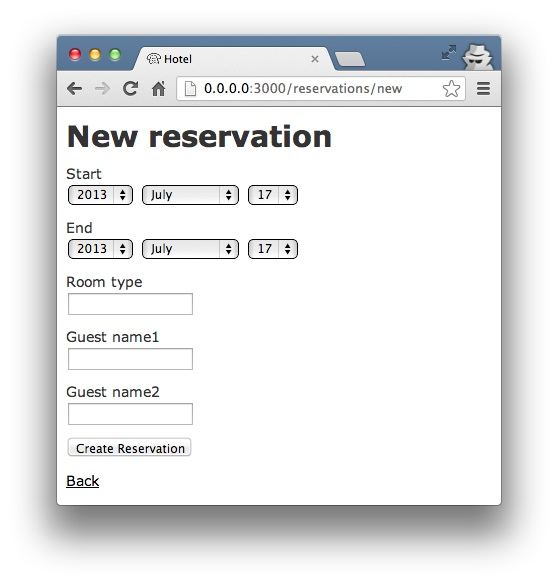
\includegraphics{screenshots/hotel_zimmer_basic_form.jpg}
\end{figure}

That is not userfriendly. The aim is to display the following page when you go to \texttt{http://0.0.0.0:3000/reservations/new}:

\begin{figure}[htbp]
\centering
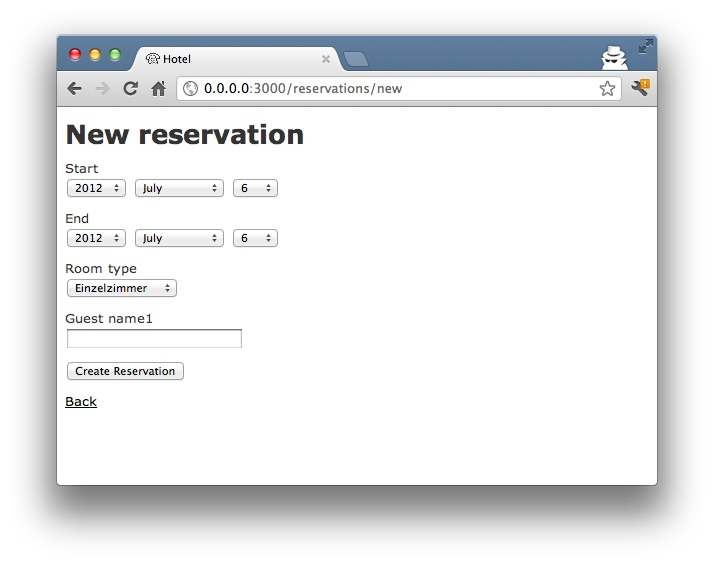
\includegraphics{screenshots/hotel_einzelzimmer_form.jpg}
\end{figure}

As soon as the user selects a double room instead of a single, we want a second name field to appear:

\begin{figure}[htbp]
\centering
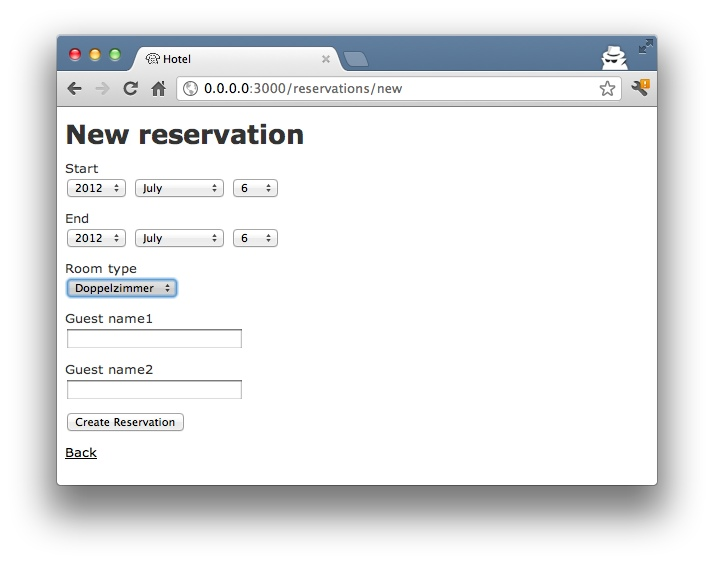
\includegraphics{screenshots/hotel_doppelzimmer_form.jpg}
\end{figure}

So I am changing two things in the \texttt{app/views/reservations/\_form.html.erb}:

\begin{itemize}
\itemsep1pt\parskip0pt\parsep0pt
\item
  Set the \texttt{room\_type} via a dropdown box. \texttt{\textless{}\%= f.select :room\_type,             options\_for\_select({[}'single room', 'double room'{]})             \%\textgreater{}}
\item
  In the div element around the second name, I set an ID `second\_name'. \texttt{\textless{}div class="field"             id='second\_name'\textgreater{}}
\end{itemize}

Here is the whole new code for \texttt{app/views/reservations/\_form.html.erb}

\begin{shaded}\begin{verbatim}
<%= form_for(@reservation) do |f| %>
  <% if @reservation.errors.any? %>
    <div id="error_explanation">
      <h2><%= pluralize(@reservation.errors.count, "error") %> prohibited this reservation from being saved:</h2>

      <ul>
      <% @reservation.errors.full_messages.each do |msg| %>
        <li><%= msg %></li>
      <% end %>
      </ul>
    </div>
  <% end %>

  <div class="field">
    <%= f.label :start %><br>
    <%= f.date_select :start %>
  </div>
  <div class="field">
    <%= f.label :end %><br>
    <%= f.date_select :end %>
  </div>
  <div class="field">
    <%= f.label :room_type %><br>
    <%= f.select :room_type, options_for_select(['single room', 'double room']) %>
  </div>
  <div class="field">
    <%= f.label :guest_name1 %><br>
    <%= f.text_field :guest_name1 %>
  </div>
  <div class="field" id='second_name'>
    <%= f.label :guest_name2 %><br>
    <%= f.text_field :guest_name2 %>
  </div>
  <div class="actions">
    <%= f.submit %>
  </div>
<% end %>
\end{verbatim}\end{shaded}

In the file \texttt{app/assets/javascripts/reservations.js.coffee} I define the CoffeeScript code that toggles the element with the ID \texttt{second\_name} between visible (\texttt{show}) or invisible (\texttt{hide}) depending on the content of \texttt{reservation\_room\_type}:

\begin{shaded}\begin{verbatim}
ready = ->
  $('#second_name').hide()
  $('#reservation_room_type').change ->
    room_type = $('#reservation_room_type :selected').text()
    if room_type == 'single room'
      $('#second_name').hide()
    else
      $('#second_name').show()

$(document).ready(ready)
$(document).on('page:load', ready)
\end{verbatim}\end{shaded}

\section{Note}\label{note-52}

In reality, you would surely integrate the guest names in a 1:n has\_many association, but in this example we just want to demonstrate how you can change the content of a form via JavaScript.

\chap{Forms}\label{forms}

\section{The Data-Input Workflow}\label{the-data-input-workflow}

To understand forms we take a look at the data workflow. Understanding it better will help to understand the work of forms.

Example application:

\begin{shaded}\begin{verbatim}
$ rails new testapp
[...]
$ cd testapp
$ rails generate scaffold Person first_name last_name
[...]
$ rake db:migrate
[...]
$ rails s
=> Booting WEBrick
=> Rails 4.0.0 application starting in development on http://0.0.0.0:3000
=> Run `rails server -h` for more startup options
=> Ctrl-C to shutdown server
[2013-07-20 09:48:23] INFO  WEBrick 1.3.1
[2013-07-20 09:48:23] INFO  ruby 2.0.0 (2013-06-27) [x86_64-darwin12.4.0]
[2013-07-20 09:48:23] INFO  WEBrick::HTTPServer#start: pid=72655 port=3000
\end{verbatim}\end{shaded}

Most times we create forms by using the Scaffold. Let's go through the flow the data

\chap{Request the people\#new form}\label{request-the-peoplenew-form}

Wenn we request the \texttt{http://0.0.0.0:3000/people/new} URL the router answers the following route:

\begin{shaded}\begin{verbatim}
new_person GET    /people/new(.:format)      people#new
\end{verbatim}\end{shaded}

The controller \texttt{app/controllers/people\_controller.rb} runs this code:

\begin{shaded}\begin{verbatim}
## GET /people/new
def new
  @person = Person.new
end
\end{verbatim}\end{shaded}

So a new Instance of Person is created and stored in the instance variable \texttt{@person}.

Rails takes \texttt{@person} and starts processing the view file \texttt{app/views/people/new.html.erb}

\begin{shaded}\begin{verbatim}
<h1>New person</h1>

<%= render 'form' %>

<%= link_to 'Back', people_path %>
\end{verbatim}\end{shaded}

\texttt{render 'form'} renders the file \texttt{app/views/people/\_form.html.erb}

\begin{shaded}\begin{verbatim}
<%= form_for(@person) do |f| %>
  [...]
    <%= f.text_field :first_name %>
  [...]
    <%= f.text_field :last_name %>
  [...]
    <%= f.submit %>
  [...]
<% end %>
\end{verbatim}\end{shaded}

\texttt{form\_for(@person)} embeddeds the two text\_fields \texttt{:first\_name} and \texttt{:last\_name} plus a \texttt{submit} Button.

The resulting HTML:

\begin{shaded}\begin{verbatim}
[...]
<form accept-charset="UTF-8" action="/people" class="new_person" id="new_person" method="post">
  [...]
    <input id="person_first_name" name="person[first_name]" type="text" />
  [...]
    <input id="person_last_name" name="person[last_name]" type="text" />
  [...]
    <input name="commit" type="submit" value="Create Person" />
  [...]
</form>
[...]
\end{verbatim}\end{shaded}

This form uses the \texttt{post} method to upload the data to the server.

\section{Push the Data to the Server}\label{push-the-data-to-the-server}

We enter `Stefan' in the \texttt{first\_name} field and `Wintermeyer' in the \texttt{last\_name} field and click the submit button. The browser uses the post method to uploads the data to the URL \texttt{/people}. The log shows:

\begin{shaded}\begin{verbatim}
Started POST "/people" for 127.0.0.1 at 2013-07-20 10:14:02 +0200
Processing by PeopleController#create as HTML
  Parameters: {"utf8"=>"✓", "authenticity_token"=>"cIZ+XFBx75mnXb6WiVv4xj6S88ahPjwVedDg1YgGuJs=", "person"=>{"first_name"=>"Stefan", "last_name"=>"Wintermeyer"}, "commit"=>"Create Person"}
   (0.1ms)  begin transaction
  SQL (4.6ms)  INSERT INTO "people" ("created_at", "first_name", "last_name", "updated_at") VALUES (?, ?, ?, ?)  [["created_at", Sat, 20 Jul 2013 08:14:02 UTC +00:00], ["first_name", "Stefan"], ["last_name", "Wintermeyer"], ["updated_at", Sat, 20 Jul 2013 08:14:02 UTC +00:00]]
   (0.9ms)  commit transaction
Redirected to http://0.0.0.0:3000/people/1
Completed 302 Found in 10ms (ActiveRecord: 5.5ms)
\end{verbatim}\end{shaded}

What happend in Rails?

The router answers the request with this route

\begin{shaded}\begin{verbatim}
POST   /people(.:format)          people#create
\end{verbatim}\end{shaded}

The controller \texttt{app/controllers/people\_controller.rb} runs this code

\begin{shaded}\begin{verbatim}
## POST /people
## POST /people.json
def create
  @person = Person.new(person_params)
  [...]
    if @person.save
      format.html { redirect_to @person, notice: 'Person was successfully created.' }
    [...]
    end
  end
end
[...]

## Never trust parameters from the scary internet, only allow the white list through.
def person_params
  params.require(:person).permit(:first_name, :last_name)
end
\end{verbatim}\end{shaded}

A new instance variable \texttt{@person} is created. It represense a new Person which was created with the params that were send from the browser to the Rails application. The params are checked in the person\_params method which is a whitelist. That is done so the user can not just inject params which we don't want to be injected.

Once \texttt{@person} is saved a \texttt{redirect\_to       @person} is triggered. That would be \texttt{http://0.0.0.0:3000/people/1} in this example.

\section{Present the new Data}\label{present-the-new-data}

The redirect to \texttt{http://0.0.0.0:3000/people/1} is traceable in the log file

\begin{shaded}\begin{verbatim}
Started GET "/people/1" for 127.0.0.1 at 2013-07-20 10:14:02 +0200
Processing by PeopleController#show as HTML
  Parameters: {"id"=>"1"}
  Person Load (0.2ms)  SELECT "people".* FROM "people" WHERE "people"."id" = ? LIMIT 1  [["id", "1"]]
  Rendered people/show.html.erb within layouts/application (1.1ms)
Completed 200 OK in 9ms (Views: 5.3ms | ActiveRecord: 0.2ms)
\end{verbatim}\end{shaded}

The router answers to this request with

\begin{shaded}\begin{verbatim}
person GET    /people/:id(.:format)      people#show
\end{verbatim}\end{shaded}

Which gets handled be the show method in \texttt{app/controllers/people\_controller.rb}

\section{Generic Forms}\label{generic-forms}

A form doesn't have to be hardwired to an ActiveRecord object. You can use the \texttt{form\_tag} helper to create a form by youself. I use the example of \url{http://guides.rubyonrails.org/form_helpers.html}\{.uri\}(which is the official Rails guide about forms) to show how to create a search form which is not connected to a model:

\begin{shaded}\begin{verbatim}
<%= form_tag("/search", method: "get") do %>
  <%= label_tag(:q, "Search for:") %>
  <%= text_field_tag(:q) %>
  <%= submit_tag("Search") %>
<% end %>
\end{verbatim}\end{shaded}

It results in this HTML code:

\begin{shaded}\begin{verbatim}
<form accept-charset="UTF-8" action="/search" method="get">
  <label for="q">Search for:</label>
  <input id="q" name="q" type="text" />
  <input name="commit" type="submit" value="Search" />
</form>
\end{verbatim}\end{shaded}

To handle this you'd have to create a new route in \texttt{config/routes.rb} and write a method in a controller to handle it.

\section{FormTagHelper}\label{formtaghelper}

There is not just a helper for text fields. Have a look at the offical API documentation for all FormTagHelpers at \url{http://api.rubyonrails.org/classes/ActionView/Helpers/FormTagHelper.html}\{.uri\} to get an overview. Because normaly we use Scaffold to create a form there is no need to memorize them. It is just important to know where to look in case you need something else.

\chap{Alternatives}\label{alternatives}

Many Rails developer use Simple Form as an alternative to the standard way of defining forms. It is worth a try because you can really safe time and most of the times it is just easier. Simple Form is available as a Gem at \texttt{https://github.com/plataformatec/simple\_form}

\chap{Caching}\label{caching}

\section{Introduction}\label{introduction-7}

Where caching of web applications is concerned, most people tend to wait until they encounter performance problems. Then the admin first looks at the database and adds an index here and there. If that does not help, he has a look at the views and adds fragment caching. But this is not the best approach for working with caches. The aim of this chapter is to help you understand how key based cache expiration works. You can then use this approach to plan new applications already on the database structure level in such a way that you can cache optimally during development.

There are two main arguments for using caching:

\begin{itemize}
\itemsep1pt\parskip0pt\parsep0pt
\item
  The application becomes faster for the user. A faster web page results in happier users.
\item
  You need less hardware for the web server, because you require less resources for processing the queries. On average, a well cached system only needs a fifth of the processing power of a non-cached system. Quite often, it is even less.
\end{itemize}

If these two arguments are irrelevant for you, then you do not need to read this chapter.

We are going to look at three different caching methods:

\begin{itemize}
\itemsep1pt\parskip0pt\parsep0pt
\item
  HTTP caching This is the sledge hammer among the caching methods and the ultimate performance weapon. In particular, web pages that are intended for mobile devices (for example iPhone) should try to make the most of HTTP caching. If you use a combination of key based cache expiration and HTTP caching, you save a huge amount of processing time on the server and also bandwidth.
\item
  Page caching This is the screwdriver among the caching methods. You can get a lot of performance out of the system, but it is not as good as HTTP caching.
\item
  Fragment caching The tweezers among the caching methods, so to speak. But don't underestimate it. Every little helps.
\end{itemize}

\subsection{Tip}\label{tip-19}

The aim is to optimally combine all three methods.

\section{A Simple Example Application}\label{a-simple-example-application}

To try out the caching methods, we need an example application. We are going to use a simple phone book with a model for the company and a model for the employees of the company.

\subsection{Important}\label{important-15}

Please consider: if the processing power you save (shown later) is already so significant in such a simple application, it will be even more significant in a more complex application with more complex views.

We create the new Rails app:

\begin{shaded}\begin{verbatim}
$ rails new phone_book
  [...]
$ cd phone_book
$ rails generate scaffold company name
  [...]
$ rails generate scaffold employee company_id:integer last_name first_name phone_number
  [...]
$ rake db:migrate
  [...]
$
\end{verbatim}\end{shaded}

\section{Models}\label{models}

We insert a few rudimentary rules in the two models.

\texttt{app/models/company.rb}

\begin{shaded}\begin{verbatim}
class Company < ActiveRecord::Base
  validates :name,
            presence: true,
            uniqueness: true

  has_many :employees, dependent: :destroy

  def to_s
    name
  end
end
\end{verbatim}\end{shaded}

\texttt{app/models/employee.rb}

\begin{shaded}\begin{verbatim}
class Employee < ActiveRecord::Base
  belongs_to :company, touch: true

  validates :first_name,
            presence: true

  validates :last_name,
            presence: true

  validates :company,
            presence: true

  def to_s
    "#{first_name} #{last_name}"
  end
end
\end{verbatim}\end{shaded}

\section{Views}\label{views}

We change the following two company views to list the number of employees in the Index view and all the employees in the Show view.

\texttt{app/views/companies/index.html.erb}

\begin{shaded}\begin{verbatim}
<h1>Listing companies</h1>

<table>
  <thead>
    <tr>
      <th>Name</th>
      <th>Number of employees</th>
      <th></th>
      <th></th>
      <th></th>
    </tr>
  </thead>

  <tbody>
    <% @companies.each do |company| %>
      <tr>
        <td><%= company.name %></td>
        <td><%= company.employees.count %></td>
        <td><%= link_to 'Show', company %></td>
        <td><%= link_to 'Edit', edit_company_path(company) %></td>
        <td><%= link_to 'Destroy', company, method: :delete, data: { confirm: 'Are you sure?' } %></td>
      </tr>
    <% end %>
  </tbody>
</table>

<br>

<%= link_to 'New Company', new_company_path %>
\end{verbatim}\end{shaded}

\texttt{app/views/companies/show.html.erb}

\begin{shaded}\begin{verbatim}
<p id="notice"><%= notice %></p>

<p>
  <strong>Name:</strong>
  <%= @company.name %>
</p>

<%= link_to 'Edit', edit_company_path(@company) %> |
<%= link_to 'Back', companies_path %>

<h1>Listing employees</h1>

<table>
  <thead>
    <tr>
      <th>Last name</th>
      <th>First name</th>
      <th>Phone number</th>
    </tr>
  </thead>

  <tbody>
    <% @company.employees.each do |employee| %>
      <tr>
        <td><%= employee.last_name %></td>
        <td><%= employee.first_name %></td>
        <td><%= employee.phone_number %></td>
      </tr>
    <% end %>
  </tbody>
</table>
\end{verbatim}\end{shaded}

\section{Example Data}\label{example-data}

To easily populate the database, we use the Faker gem (see \url{http://faker.rubyforge.org/}\{.uri\}). With Faker, you can generate random names and phone numbers. Please add the following line in the \texttt{Gemfile}:

\begin{shaded}\begin{verbatim}
gem 'faker'
\end{verbatim}\end{shaded}

Then start a \textbf{bundle install}:

\begin{shaded}\begin{verbatim}
$ bundle install
[...]
$
\end{verbatim}\end{shaded}

In the \texttt{db/seeds.rb} we create 30 companies with a random number of employees in each case:

\begin{shaded}\begin{verbatim}
30.times do
  company = Company.new(:name => Faker::Company.name)
  if company.save
    SecureRandom.random_number(100).times do
      company.employees.create(
                               first_name:   Faker::Name.first_name,
                               last_name:    Faker::Name.last_name,
                               phone_number: Faker::PhoneNumber.phone_number
                              )
    end
  end
end
\end{verbatim}\end{shaded}

We populate it via \textbf{rake db:seed}

\begin{shaded}\begin{verbatim}
$ rake db:seed
$
\end{verbatim}\end{shaded}

You can start the application with \textbf{rails server} and retrieve the example data with a web browser by going to the URLs \texttt{http://0.0.0.0:3000/companies} and \texttt{http://0.0.0.0:3000/companies/1}.

\chap{Normal Speed of the Pages to Optimize}\label{normal-speed-of-the-pages-to-optimize}

In this chapter, we optimize the following web pages. Start the Rails application in development mode with \textbf{rails server}. The relevant numbers of course depend on the hardware you are using.

\begin{shaded}\begin{verbatim}
$ rails server
=> Booting WEBrick
=> Rails 4.0.0 application starting in development on http://0.0.0.0:3000
=> Run `rails server -h` for more startup options
=> Ctrl-C to shutdown server
[2013-07-17 23:50:11] INFO  WEBrick 1.3.1
[2013-07-17 23:50:11] INFO  ruby 2.0.0 (2013-06-27) [x86_64-darwin12.4.0]
[2013-07-17 23:50:11] INFO  WEBrick::HTTPServer#start: pid=43210 port=3000
\end{verbatim}\end{shaded}

To access the web pages, we use the command line tool curl (\url{http://curl.haxx.se/}\{.uri\}). Of course you can also access the web pages with other web browsers. We look at the time shown in the Rails log for creating the page. In reality, you need to add the time it takes for the page to be delivered to the web browser.

\section{List of All Companies (Index View)}\label{list-of-all-companies-index-view}

At the URL \texttt{http://0.0.0.0:3000/companies} the user can see a list of all saved companies with the relevant number of employees.

Generating the page takes 48ms.

\begin{shaded}\begin{verbatim}
Completed 200 OK in 48ms (Views: 38.9ms | ActiveRecord: 8.3ms)
\end{verbatim}\end{shaded}

\section{Detailled View of a Single Company (Show View)}\label{detailled-view-of-a-single-company-show-view}

At the URL \texttt{http://0.0.0.0:3000/companies/1} the user can see the details of the first company with all employees.

Generating the page takes 11ms.

\begin{shaded}\begin{verbatim}
Completed 200 OK in 11ms (Views: 8.6ms | ActiveRecord: 0.8ms)
\end{verbatim}\end{shaded}

\section{HTTP Caching}\label{http-caching}

HTTP caching attempts to reuse already loaded web pages or files. For example, if you visit a web page such as \url{http://www.heise.de}\{.uri\} or \url{http://www.spiegel.de}\{.uri\} several times a day to read the latest news, then certain elements of that page (for example, the logo image at the top of the page) will not be loaded again on your second visit. Your browser already has these files in the cache, which saves loading time and bandwidth.

Within the Rails framework, our aim is answering the question “Has a page changed?” already in the controller. Because normally, most of the time is spent on rendering the page in the view. I'd like to repeat that: Most of the time is spent on rendering the page in the view!

\section{Last-Modified}\label{last-modified}

\subsection{Important}\label{important-16}

Please modify the times used in the examples in accordance with your own local circumstances.

The web browser knows when it has downloaded a web page and then placed it into the cache. It can pass this information to the web server in an \texttt{If-Modified-Since:} header. The web server can then compare this information to the corresponding file and either deliver a newer version or return an HTTP 304 Not Modified code as response. In case of a 304, the web server delivers the cached version. Now you are going to say, “That's all very well for images, but it won't help me at all for dynamically generated web pages such as the Index view of the companies.” Ah, but you are underestimating what Rails can do. ;-)

Please edit the \texttt{show} method in the controller file \texttt{app/controllers/companies\_controller.rb} as follows :

\begin{shaded}\begin{verbatim}
## GET /companies/1
# GET /companies/1.json
def show
  fresh_when last_modified: @company.updated_at
end
\end{verbatim}\end{shaded}

After restarting the Rails application, we have a look at the HTTP header of \texttt{http://0.0.0.0:3000/companies/1}:

\begin{shaded}\begin{verbatim}
$ curl -I http://0.0.0.0:3000/companies/1
HTTP/1.1 200 OK
X-Frame-Options: SAMEORIGIN
X-Xss-Protection: 1; mode=block
X-Content-Type-Options: nosniff
X-Ua-Compatible: chrome=1
Last-Modified: Wed, 17 Jul 2013 21:50:01 GMT
[...]
$
\end{verbatim}\end{shaded}

The \texttt{Last-Modified} entry in the HTTP header was generated by \texttt{fresh\_when} in the controller. If we later go to the same web page and specify this time as well, then we do not get the web page back, but a \texttt{304 Not Modified} message:

\begin{shaded}\begin{verbatim}
$ curl -I http://0.0.0.0:3000/companies/1 --header 'If-Modified-Since: Wed, 17 Jul 2013 21:50:01 GMT'
HTTP/1.1 304 Not Modified
[...]
$
\end{verbatim}\end{shaded}

In the Rails log, we find this:

\begin{shaded}\begin{verbatim}
Started HEAD "/companies/1" for 127.0.0.1 at 2013-07-18 08:27:10 +0200
Processing by CompaniesController#show as */*
  Parameters: {"id"=>"1"}
  Company Load (0.1ms)  SELECT "companies".* FROM "companies" WHERE "companies"."id" = ? LIMIT 1  [["id", "1"]]
Completed 304 Not Modified in 2ms (ActiveRecord: 0.1ms)
\end{verbatim}\end{shaded}

Rails took 2ms to answer this request, compared to the 11ms of the standard variation. This is way faster! So you have used less resources on the server. And saved a massive amount of bandwidth. The user will be able to see the page much more quickly.

\chap{Etag}\label{etag}

Sometimes the \texttt{update\_at} field of a particular object is not meaningful on its own. For example, if you have a web page where users can log in and this page then generates web page contents based on a role model, it can happen that user A as admin is able to see an Edit link that is not displayed to user B as normal user. In such a scenario, the Last-Modified header explained in \hyperref[httpux5fcachingux5flastux5fmodified]{the section called “Last-Modified”} does not help.

In these cases, we can use the etag header. The etag is generated by the web server and delivered when the web page is first visited. If the user visits the same URL again, the browser can then check if the corresponding web page has changed by sending a \texttt{If-None-Match:} query to the web server.

Please edit the \texttt{index} and \texttt{show} methods in the controller file \texttt{app/controllers/companies\_controller.rb} as follows:

\begin{shaded}\begin{verbatim}
## GET /companies
## GET /companies.json
def index
  @companies = Company.all
  fresh_when etag: @companies
end

## GET /companies/1
## GET /companies/1.json
def show
  fresh_when etag: @company
end
\end{verbatim}\end{shaded}

A special Rails feature comes into play for the etag: Rails automatically sets a new CSRF token for each new visitor of the website. This prevents cross-site request forgery attacks (see \url{http://en.wikipedia.org/wiki/Cross_site_request_forgery}\{.uri\}). But it also means that each new user of a web page gets a new etag for the same page. To ensure that the same users also get identical CSRF tokens, these are stored in a cookie by the web browser and consequently sent back to the web server every time the web page is visited. The curl we used for developing does not do this by default. But we can tell curl that we want to save all cookies in a file and transmit these cookies later if a request is received.

For saving, we use the \texttt{-c cookies.txt} parameter.

\begin{shaded}\begin{verbatim}
$ curl -I http://0.0.0.0:3000/companies -c cookies.txt
HTTP/1.1 200 OK
X-Frame-Options: SAMEORIGIN
X-Xss-Protection: 1; mode=block
X-Content-Type-Options: nosniff
X-Ua-Compatible: chrome=1
Etag: "e57e45d14a0afc4377c81fc5ecc951b0"
[...]

$
\end{verbatim}\end{shaded}

With the parameter \texttt{-b cookies.txt}, curl sends these cookies to the web server when a request arrives. Now we get the same etag for two subsequent requests:

\begin{shaded}\begin{verbatim}
$ curl -I http://0.0.0.0:3000/companies -b cookies.txt
HTTP/1.1 200 OK
X-Frame-Options: SAMEORIGIN
X-Xss-Protection: 1; mode=block
X-Content-Type-Options: nosniff
X-Ua-Compatible: chrome=1
Etag: "e57e45d14a0afc4377c81fc5ecc951b0"
[...]

$ curl -I http://0.0.0.0:3000/companies -b cookies.txt
HTTP/1.1 200 OK
X-Frame-Options: SAMEORIGIN
X-Xss-Protection: 1; mode=block
X-Content-Type-Options: nosniff
X-Ua-Compatible: chrome=1
Etag: "e57e45d14a0afc4377c81fc5ecc951b0"
[...]

$
\end{verbatim}\end{shaded}

We now use this etag to find out in the request with \texttt{If-None-Match} if the version we have cached is still up to date:

\begin{shaded}\begin{verbatim}
$ curl -I http://0.0.0.0:3000/companies -b cookies.txt --header 'If-None-Match: "e57e45d14a0afc4377c81fc5ecc951b0"'
HTTP/1.1 304 Not Modified
X-Frame-Options: SAMEORIGIN
X-Xss-Protection: 1; mode=block
X-Content-Type-Options: nosniff
X-Ua-Compatible: chrome=1
Etag: "e57e45d14a0afc4377c81fc5ecc951b0"
[...]

$
\end{verbatim}\end{shaded}

We get a \texttt{304 Not Modified} in response. Let's look at the Rails log:

\begin{shaded}\begin{verbatim}
Started HEAD "/companies" for 127.0.0.1 at 2013-07-18 08:32:43 +0200
Processing by CompaniesController#index as */*
  Company Load (0.3ms)  SELECT "companies".* FROM "companies"
Completed 304 Not Modified in 4ms (ActiveRecord: 0.3ms)
\end{verbatim}\end{shaded}

Rails only took 4ms to process the request. Almost 10 times as fast as the variation without cache! Plus we have saved bandwidth again. The user will be happy with the speedy web application.

\section{current\_user and Other Potential Parameters}\label{currentux5fuser-and-other-potential-parameters}

As basis for generating an etag, we can not just pass an object, but also an array of objects. This way, we can solve the problem with the logged-in user. Let's assume that a logged-in user is output with the method \texttt{current\_user}.

We only have to add \texttt{etag \{ current\_user.try :id \}} in the \texttt{app/controllers/application\_controller.rb} to make sure that all etags in the application include the current\_user.id which is nil in case nobody is logged in.

\begin{shaded}\begin{verbatim}
class ApplicationController < ActionController::Base
  ## Prevent CSRF attacks by raising an exception.
  # For APIs, you may want to use :null_session instead.
  protect_from_forgery with: :exception

  etag { current_user.try :id }
end
\end{verbatim}\end{shaded}

You can chain other objects in this array too and use this approach to define when a page has not changed.

\section{The Magic of touch}\label{the-magic-of-touch}

What happens if an \texttt{Employee} is edited or deleted? Then the show view and potentially also the index view would have to change as well. That is the reason for the line

\begin{shaded}\begin{verbatim}
belongs_to :company, touch: true
\end{verbatim}\end{shaded}

in the employee model. Every time an object of the class \texttt{Employee} is saved in edited form, and if \texttt{touch: true} is used, ActiveRecord updates the superordinate \texttt{Company} element in the database. The \texttt{updated\_at} field is set to the current time. It is “touched”.

This approach ensures that a correct content is delivered.

\section{stale?}\label{stale}

Up to now, we have always assumed that only HTML pages are deliverd. So we were able to use \texttt{fresh\_when} and then do without the \texttt{respond\_to do \textbar{}format\textbar{}} block. But HTTP caching is not limited to HTML pages. Yet if we render JSON (for example) as well and want to deliver it via HTTP caching, we need to use the method \texttt{stale?}. Using \texttt{stale?} resembles using the method \texttt{fresh\_when}. Example:

\begin{shaded}\begin{verbatim}
def show
  @company = Company.find(params[:id])

  if stale? @company
    respond_to do |format|
      format.html
      format.json { render json: @company }
    end
  end
end
\end{verbatim}\end{shaded}

\section{Using Proxies (public)}\label{using-proxies-public}

Up to now, we always assumed that we are using a cache on the web browser. But on the Internet, there are many proxies that are often closer to the user and can therefore useful for caching in case of non-personalized pages. If our example was a publicly accessible phone book, then we could activate the free services of the proxies with the parameter \texttt{public: true} in \texttt{fresh\_when} or \texttt{stale?}.

Example:

\begin{shaded}\begin{verbatim}
## GET /companies/1
## GET /companies/1.json
def show
  @company = Company.find(params[:id])

  fresh_when @company, public: true
end
\end{verbatim}\end{shaded}

We go to the web page and get the output:

\begin{shaded}\begin{verbatim}
$ curl -I http://0.0.0.0:3000/companies/1
HTTP/1.1 200 OK
X-Frame-Options: SAMEORIGIN
X-Xss-Protection: 1; mode=block
X-Content-Type-Options: nosniff
X-Ua-Compatible: chrome=1
Etag: "81cfb867cac24fad7ff1a7721bfb529a"
Last-Modified: Wed, 17 Jul 2013 21:50:01 GMT
Content-Type: text/html; charset=utf-8
Cache-Control: public
[...]
\end{verbatim}\end{shaded}

The header \texttt{Cache-Control: public} tells all proxies that they can also cache this web page.

\subsection{Warning}\label{warning-14}

Using proxies always has to be done with great caution. On the one hand, they are brilliantly suited for delivering your own web page quickly to more users, but on the other, you have to be absolutely sure that no personalized pages are cached on public proxies. For example, CSRF tags and Flash messages should never end up in a public proxy. To be sure with the CSRF tags, it is a good idea to make the output of \texttt{csrf\_meta\_tag} in the default \texttt{app/views/layouts/application.html.erb} layout dependent on the question whether the page may be cached publicly or not:

\begin{shaded}\begin{verbatim}
<%= csrf_meta_tag unless response.cache_control[:public] %>
\end{verbatim}\end{shaded}

\chap{Cache-Control With Time Limit}\label{cache-control-with-time-limit}

When using \texttt{Etag} and \texttt{Last-Modified} we assume in \hyperref[httpux5fcachingux5fetag]{the section called “Etag”} and \hyperref[httpux5fcachingux5flastux5fmodified]{the section called “Last-Modified”} that the web browser definitely checks once more with the web server if the cached version of a web page is still current. This is a very safe approach.

But you can take the optimization one step further by predicting the future: if I am already sure when delivering the web page that this web page is not going to change in the next two minutes, hours or days, then I can tell the web browser this directly. It then does not need to check back again within this specified period of time. This overhead saving has advantages, especially with mobile web browsers with relatively high latency. Plus you also save server load on the web server.

In the output of the HTTP header, you may already have noticed the corresponding line in the \texttt{Etag} and \texttt{Last-Modified} examples:

\begin{shaded}\begin{verbatim}
Cache-Control: max-age=0, private, must-revalidate
\end{verbatim}\end{shaded}

The item \texttt{must-revalidate} tells the web browser that it should definitely check back with the web server to see if a web page has changed in the meantime. The second parameter \texttt{private} means that only the web browser is allowed to cache this page. Any proxies on the way are not permitted to cache this page.

If we decide for our phone book that the web page is going to stay unchanged for at least 2 minutes, then we can expand the code example by adding the method \texttt{expires\_in}. The controller \texttt{app/controllers/companies.rb} would then contain the following code for the method \texttt{show}:

\begin{shaded}\begin{verbatim}
## GET /companies/1
## GET /companies/1.json
def show
  expires_in 2.minutes
  fresh_when @company, public: true
end
\end{verbatim}\end{shaded}

Now we get a different cache control information in response to a request:

\begin{shaded}\begin{verbatim}
$ curl -I http://0.0.0.0:3000/companies/1
HTTP/1.1 200 OK
X-Frame-Options: SAMEORIGIN
X-Xss-Protection: 1; mode=block
X-Content-Type-Options: nosniff
X-Ua-Compatible: chrome=1
Date: Thu, 18 Jul 2013 06:55:30 GMT
Etag: "81cfb867cac24fad7ff1a7721bfb529a"
Last-Modified: Wed, 17 Jul 2013 21:50:01 GMT
Content-Type: text/html; charset=utf-8
Cache-Control: max-age=120, public
[...]
\end{verbatim}\end{shaded}

The two minutes are specified in seconds (\texttt{max-age=120}) and we no longer need \texttt{must-revalidate}. So in the next 120 seconds, the web browser does not need to check back with the web server to see if the content of this page has changed.

\section{Note}\label{note-53}

This mechanism is also used by the asset pipeline. Assets created there in the production environment can be identified clearly by the checksum in the file name and can be cached for a very long time both in the web browser and in public proxies. That's why we have the following section in the nginx configuration file in \hyperref[railsux5fproductionux5fwebserver]{Chapter~16, \emph{Web Server in Production Mode}}:

\begin{shaded}\begin{verbatim}
location ^~ /assets/ {
  gzip_static on;
  expires max;
  add_header Cache-Control public;
}
\end{verbatim}\end{shaded}

\chap{Fragment Caching}\label{fragment-caching}

With fragment caching you can cache individual parts of a view. You can safely use it in combination with \hyperref[httpux5fcaching]{the section called “HTTP Caching”} and \hyperref[pageux5fcaching]{the section called “Page Caching”}. The advantages once again are a reduction of server load and faster web page generation, which means increased usability.

Please install a new example application (see \hyperref[cachingux5fbeispielapplikation]{the section called “A Simple Example Application”}).

\section{Enabling Fragment Caching in Development Mode}\label{enabling-fragment-caching-in-development-mode}

First, we need to go to the file \texttt{config/environments/development.rb} and set the item \texttt{config.action\_controller.perform\_caching} to \texttt{true}:

\begin{shaded}\begin{verbatim}
config.action_controller.perform_caching = true
\end{verbatim}\end{shaded}

Otherwise, we cannot try out the fragment caching in development mode. In production mode, fragment caching is enabled by default.

\section{Caching Table of Index View}\label{caching-table-of-index-view}

On the page \texttt{http://0.0.0.0:3000/companies}, a very computationally intensive table with all companies is rendered. We can cache this table as a whole. To do so, we need to enclose the table in a \texttt{\textless{}\% cache('name\_of\_cache') do \%\textgreater{} ... \textless{}\% end       \%\textgreater{}} block:

\begin{shaded}\begin{verbatim}
<% cache('name_of_cache') do %>

[...]

<% end %>
\end{verbatim}\end{shaded}

Please edit the file \texttt{app/views/companies/index.html.erb} as follows:

\begin{shaded}\begin{verbatim}
<h1>Listing companies</h1>

<% cache('table_of_all_companies') do %>
<table>
  <thead>
    <tr>
      <th>Name</th>
      <th>Number of employees</th>
      <th></th>
      <th></th>
      <th></th>
    </tr>
  </thead>

  <tbody>
    <% @companies.each do |company| %>
      <tr>
        <td><%= company.name %></td>
        <td><%= company.employees.count %></td>
        <td><%= link_to 'Show', company %></td>
        <td><%= link_to 'Edit', edit_company_path(company) %></td>
        <td><%= link_to 'Destroy', company, method: :delete, data: { confirm: 'Are you sure?' } %></td>
      </tr>
    <% end %>
  </tbody>
</table>
<% end %>

<br />

<%= link_to 'New Company', new_company_path %>
\end{verbatim}\end{shaded}

Then you can start the Rails server with \textbf{rails server} and go to the URL \texttt{http://0.0.0.0:3000/companies}. In the development log, you will now see the following entry:

\begin{shaded}\begin{verbatim}
Write fragment views/table_of_all_companies (2.9ms)
  Rendered companies/index.html.erb within layouts/application (119.8ms)
Completed 200 OK in 209ms (Views: 143.1ms | ActiveRecord: 15.0ms)
\end{verbatim}\end{shaded}

Writing the cache took 2.9 ms. In total, rendering the page took 209 ms.

If you repeatedly go to the same page, you will get a different result in the log:

\begin{shaded}\begin{verbatim}
Read fragment views/table_of_all_companies (0.2ms)
  Rendered companies/index.html.erb within layouts/application (0.8ms)
Completed 200 OK in 37ms (Views: 34.6ms | ActiveRecord: 0.3ms)
\end{verbatim}\end{shaded}

Reading the cache took 0.2 ms and rendering the page in total 37ms. Only a fifth of the processing time!

\chap{Deleting Fragment Cache}\label{deleting-fragment-cache}

With the method \texttt{expire\_fragment} you can clear specific fragment caches. Basically, we can build this idea into the model in the same way as shown in \hyperref[pageux5fcachesux5fautomatischux5floeschen]{the section called “Deleting Page Caches Automatically”}.

The model file \texttt{app/models/company.rb} would then look like this:

\begin{shaded}\begin{verbatim}
class Company < ActiveRecord::Base
  validates :name,
            presence: true,
            uniqueness: true

  has_many :employees, dependent: :destroy

  after_create   :expire_cache
  after_update   :expire_cache
  before_destroy :expire_cache

  def to_s
    name
  end

  def expire_cache
    ActionController::Base.new.expire_fragment('table_of_all_companies')
  end
end
\end{verbatim}\end{shaded}

As the number of employees also has an effect on this table, we would also have to expand the file \texttt{app/models/employees.rb} accordingly:

\begin{shaded}\begin{verbatim}
class Employee < ActiveRecord::Base
  belongs_to :company, touch: true

  validates :first_name,
            presence: true

  validates :last_name,
            presence: true

  validates :company,
            presence: true

  after_create   :expire_cache
  after_update   :expire_cache
  before_destroy :expire_cache

  def to_s
    "#{first_name} #{last_name}"
  end

  def expire_cache
    ActionController::Base.new.expire_fragment('table_of_all_companies')
  end  
end
\end{verbatim}\end{shaded}

Deleting specific fragment caches often involves a lot of effort in terms of programming. One, you often miss things and two, in big projects it's not easy to keep track of all the different cache names. Often it is easier to automatically create names via the method \texttt{cache\_key}. These then expire automatically in the cache (see \hyperref[fragmentux5fautoux5fexpiring]{the section called “Auto-Expiring Caches”}).

\chap{Auto-Expiring Caches}\label{auto-expiring-caches}

Managing fragment caching is rather complex with the naming convention used in \hyperref[fragmentux5fcachingux5ftabelleux5fcachen]{the section called “Caching Table of Index View”}. On the one hand, you can be sure that the cache does not have any superfluous ballast if you have programmed neatly, but on the other, it does not really matter. A cache is structured in such a way that it deletes old and no longer required elements on its own. If we use a mechanism that gives a fragment cache a unique name, as in the asset pipeline (see \hyperref[assetux5fpipeline]{Chapter~12, \emph{Asset Pipeline}}), then we would not need to go to all the trouble of deleting fragment caches.

That is precisely what the method \texttt{cache\_key} is for. \texttt{cache\_key} gives you a unique name for an element. Let's try it in the console. First, we get the always identical \texttt{cache\_key} of the first company item two times in a row (“companies/1-20130717215001729269000”), then we touch the item (a \texttt{touch} sets the attribute \texttt{updated\_at} to the current time) and finally we output the new \texttt{cache\_key} (“companies/1-20130718081128853737000”):

\begin{shaded}\begin{verbatim}
$ rails console
Loading development environment (Rails 4.0.0)
>> Company.first.cache_key
  Company Load (0.1ms)  SELECT "companies".* FROM "companies" ORDER BY "companies"."id" ASC LIMIT 1
=> "companies/1-20130717215001729269000"
>> Company.first.cache_key
  Company Load (0.3ms)  SELECT "companies".* FROM "companies" ORDER BY "companies"."id" ASC LIMIT 1
=> "companies/1-20130717215001729269000"
>> Company.first.touch
  Company Load (0.2ms)  SELECT "companies".* FROM "companies" ORDER BY "companies"."id" ASC LIMIT 1
  SQL (4.2ms)  UPDATE "companies" SET "updated_at" = '2013-07-18 08:11:28.853737' WHERE "companies"."id" = 1
=> true
>> Company.first.cache_key
  Company Load (0.4ms)  SELECT "companies".* FROM "companies" ORDER BY "companies"."id" ASC LIMIT 1
=> "companies/1-20130718081128853737000"
>> exit
$
\end{verbatim}\end{shaded}

Let's use this knowledge to edit the index view in the file \texttt{app/views/companies/index.html.erb}:

\begin{shaded}\begin{verbatim}
<h1>Listing companies</h1>

<% cache(@companies) do %>
<table>
  <thead>
    <tr>
      <th>Name</th>
      <th>Number of employees</th>
      <th></th>
      <th></th>
      <th></th>
    </tr>
  </thead>

  <tbody>
    <% @companies.each do |company| %>
      <tr>
        <td><%= company.name %></td>
        <td><%= company.employees.count %></td>
        <td><%= link_to 'Show', company %></td>
        <td><%= link_to 'Edit', edit_company_path(company) %></td>
        <td><%= link_to 'Destroy', company, method: :delete, data: { confirm: 'Are you sure?' } %></td>
      </tr>
    <% end %>
  </tbody>
</table>
<% end %>

<br />

<%= link_to 'New Company', new_company_path %>
\end{verbatim}\end{shaded}

Here, we not only use a fragment cache for the whole table, but also one for each line. So the initial call will take longer than before. But if any individual companies change, only one line has to be re-rendered in each case.

\subsection{Note}\label{note-54}

There is no general answer to the question in how much detail you should use fragment caching. Just go ahead and experiment with it, then look in the log to see how long things take.

\section{Change Code in the View results in an expired Cache}\label{change-code-in-the-view-results-in-an-expired-cache}

Rails tracks an MD5 sum of the view you use. So if you change the file (e.g. \texttt{app/views/companies/index.html.erb}) the MD5 changes and all old caches will expire.

\section{Cache Store}\label{cache-store}

The cache store manages the stored fragment caches. If not configured otherwise, this is the Rails MemoryStore. This cache store is good for developing, but less suitable for a production system because it acts independently for each Ruby on Rails process. So if you have several Ruby on Rails processes running in parallel in the production system, each process holds its own MemoryStore.

\section{MemCacheStore}\label{memcachestore}

Most production systems use memcached (\url{http://memcached.org/}\{.uri\}) as cache store. To enable memcached as cache store in the production system, you need to add the following line in the file \texttt{config/environments/production.rb}:

\begin{shaded}\begin{verbatim}
config.cache_store = :mem_cache_store
\end{verbatim}\end{shaded}

The combination of appropriately used auto-expiring caches and memcached is an excellent recipe for a successful web page.

For a description of how to install a Rails production system with memcached, please read \hyperref[railsux5fproductionux5fwebserver]{Chapter~16, \emph{Web Server in Production Mode}}.

\chap{Other Cache Stores}\label{other-cache-stores}

In the official Rails documentation you will find a list of other cache stores at \url{http://guides.rubyonrails.org/caching_with_rails.html\#cache-stores}\{.uri\}.

\section{Page Caching}\label{page-caching}

Page Caching is extrem and was removed from the core of Rails 4.0. But it is still available as a gem.

\subsection{Important}\label{important-17}

You need quite a bit of knowledge to configure your Webserver (e.g.~Nginx or Apache).

With page caching, it's all about placing a complete HTML page (in other words, the render result of a view) into a subdirectory of the \texttt{public} directory and to have it delivered directly from there by the web server (for example Nginx) whenever the web page is visited next. Additionally, you can also save a compressed gz version of the HTML page there. A production web server will automatically deliver files below \texttt{public} itself and can also be configured so that any gz files present are delivered directly.

In complex views that may take 500ms or even more for rendering, the amount of time you save is of course considerable. As web page operator, you once more save valuable server resources and can service more visitors with the same hardware. The web page user profits from a faster delivery of the web page.

\section{Warning}\label{warning-15}

When programming your Rails application, please ensure that you also update this page itself, or delete it! You will find a description in \hyperref[pageux5fcachesux5fautomatischux5floeschen]{the section called “Deleting Page Caches Automatically”}. Otherwise, you end up with an outdated cache later.

Please also ensure that page caching rejects all URL parameters by default. For example, if you try to go to \texttt{http://0.0.0.0:3000/companies?search=abc} this automatically becomes \texttt{http://0.0.0.0:3000/companies}. But that can easily be fixed with a better route logic.

Please install a fresh example application (see \hyperref[cachingux5fbeispielapplikation]{the section called “A Simple Example Application”}) and add the gem with the following line in Gemfile.

\begin{shaded}\begin{verbatim}
gem 'actionpack-page_caching'
\end{verbatim}\end{shaded}

Now install it with the command \textbf{bundle install}.

\begin{shaded}\begin{verbatim}
$ bundle install
[...]
$
\end{verbatim}\end{shaded}

Lastly you have to tell Rails where to store the cache files. Please add the following line in your \texttt{config/application.rb} file:

\begin{shaded}\begin{verbatim}
config.action_controller.page_cache_directory = "#{Rails.root.to_s}/public/deploy"
\end{verbatim}\end{shaded}

\section{Activating Page Caching in Development Mode}\label{activating-page-caching-in-development-mode}

First we need to go to the file \texttt{config/environments/development.rb} and set the item \texttt{config.action\_controller.perform\_caching} to \texttt{true}:

\begin{shaded}\begin{verbatim}
config.action_controller.perform_caching = true
\end{verbatim}\end{shaded}

Otherwise, we cannot try the page caching in development mode. In production mode, page caching is enabled by default.

\section{Configure our Webserver}\label{configure-our-webserver}

Know you have to tell your webserver (e.g.~Nginx or Apache) that it should check the \texttt{/public/deploy} directory first before hitting the Rails application. You have to configure too, that it will deliver a gz file if one is available.

There is no one perfect way of doing it. You have to find the best way of doing it in your environment by youself.

\section{Tip}\label{tip-20}

As a quick and dirty hack for development you can set the \texttt{page\_cache\_directory} to public. Than your development system will deliver the cached page.

\begin{shaded}\begin{verbatim}
config.action_controller.page_cache_directory = "#{Rails.root.to_s}/public"
\end{verbatim}\end{shaded}

\section{Caching Company Index and Show View}\label{caching-company-index-and-show-view}

Enabling page caching happens in the controller. If we want to cache the show view for Company, we need to go to the controller \texttt{app/controllers/companies\_controller.rb} and enter the command \texttt{caches\_page :show} at the top:

\begin{shaded}\begin{verbatim}
class CompaniesController < ApplicationController
  caches_page :show

[...]
\end{verbatim}\end{shaded}

Before starting the application, the \texttt{public} directory looks like this:

\begin{shaded}\begin{verbatim}
public/
├── 404.html
├── 422.html
├── 500.html
├── favicon.ico
└── robots.txt
\end{verbatim}\end{shaded}

After starting the appliation with \textbf{rails server} and going to the URLs \texttt{http://0.0.0.0:3000/companies} and \texttt{http://0.0.0.0:3000/companies/1} via a web browser, it looks like this:

\begin{shaded}\begin{verbatim}
public
├── 404.html
├── 422.html
├── 500.html
├── deploy
│   └── companies
│       └── 1.html
├── favicon.ico
└── robots.txt
\end{verbatim}\end{shaded}

The file \texttt{public/deploy/companies/1.html} has been created by page caching.

From now on, the web server will only deliver the cached versions when these pages are accessed.

\section{gz Versions}\label{gz-versions}

If you use page cache, you should also cache directly zipped gz files. You can do this via the option \texttt{:gzip =\textgreater{} true} or use a specific compression parameter as symbol instead of \texttt{true} (for example \texttt{:best\_compression}).

The controller \texttt{app/controllers/companies\_controller.rb} would then look like this at the beginning:

\begin{shaded}\begin{verbatim}
class CompaniesController < ApplicationController
  caches_page :show, gzip: true

[...]
\end{verbatim}\end{shaded}

This automatically saves a compressed and an uncompressed version of each page cache:

\begin{shaded}\begin{verbatim}
public
├── 404.html
├── 422.html
├── 500.html
├── deploy
│   └── companies
│       ├── 1.html
│       └── 1.html.gz
├── favicon.ico
└── robots.txt
\end{verbatim}\end{shaded}

\chap{The File Extension .html}\label{the-file-extension-.html}

Rails saves the page accessed at \texttt{http://0.0.0.0:3000/companies} under the file name \texttt{companies.html}. So the upstream web server will find and deliver this file if you go to \texttt{http://0.0.0.0:3000/companies.html}, but not if you try to go to \texttt{http://0.0.0.0:3000/companies}, because the extension \texttt{.html} at the end of the URI is missing.

If you are using the Nginx server as described in \hyperref[railsux5fproductionux5fwebserver]{Chapter~16, \emph{Web Server in Production Mode}}, the easiest way is adapting the \texttt{try\_files} instruction in the Nginx configuration file as follows:

\begin{shaded}\begin{verbatim}
try_files $uri/index.html $uri $uri.html @unicorn;
\end{verbatim}\end{shaded}

Nginx then checks if a file with the extension \texttt{.html} of the currently accessed URI exists.

\chap{Deleting Page Caches Automatically}\label{deleting-page-caches-automatically}

As soon as the data used in the view changes, the saved cache files have to be deleted. Otherwise, the cache would no longer be up to date.

According to the official Rails documentation, the solution for this problem is the class \texttt{ActionController::Caching::Sweeper}. But this approach, described at \url{http://guides.rubyonrails.org/caching_with_rails.html\#sweepers}\{.uri\}, has a big disadvantage: it is limited to actions that happen within the controller. So if an action is triggered via URL by the web browser, the corresponding cache is also changed or deleted. But if an object is deleted in the console, for example, the sweeper would not realize this. For that reason, I am going to show you an approach that does not use a sweeper, but works directly in the model with ActiveRecord callbacks.

In our phone book application, we always need to delete the cache for \texttt{http://0.0.0.0:3000/companies} and \texttt{http://0.0.0.0:3000/companies/company\_id} when editing a company. When editing an employee, we also have to delete the corresponding cache for the relevant employee.

\chap{Models}\label{models-1}

Now we still need to fix the models so that the corresponding caches are deleted automatically as soon as an object is created, edited or deleted.

\texttt{app/models/company.rb}

\begin{shaded}\begin{verbatim}
class Company < ActiveRecord::Base
  validates :name,
            presence: true,
            uniqueness: true

  has_many :employees, dependent: :destroy

  after_create   :expire_cache
  after_update   :expire_cache
  before_destroy :expire_cache

  def to_s
    name
  end

  def expire_cache
    ActionController::Base.expire_page(Rails.application.routes.url_helpers.company_path(self))
    ActionController::Base.expire_page(Rails.application.routes.url_helpers.companies_path)
  end

end
\end{verbatim}\end{shaded}

\texttt{app/models/employee.rb}

\begin{shaded}\begin{verbatim}
class Employee < ActiveRecord::Base
  belongs_to :company, touch: true

  validates :first_name,
            presence: true

  validates :last_name,
            presence: true

  validates :company,
            presence: true

  after_create   :expire_cache
  after_update   :expire_cache
  before_destroy :expire_cache

  def to_s
    "#{first_name} #{last_name}"
  end

  def expire_cache
    ActionController::Base.expire_page(Rails.application.routes.url_helpers.employee_path(self))
    ActionController::Base.expire_page(Rails.application.routes.url_helpers.employees_path)
    self.company.expire_cache
  end

end
\end{verbatim}\end{shaded}

\chap{Preheating}\label{preheating}

Now that you have read your way through the caching chapter, here is a final tip: preheat your cache!

For example, if you have a web application in a company and you know that at 9 o'clock in the morning, all employees are going to log in and then access this web application, then it's a good idea to let your web server go through all those views a few hours in advance with cron-job. At night, your server is probably bored anyway.

Check out the behavior patterns of your users. With public web pages, this can be done for example via Google Analytics (\url{http://www.google.com/analytics/}\{.uri\}). You will find that at certain times of the day, there is a lot more traffic going in. If you have a quiet phase prior to this, you can use it to warm up your cache.

The purpose of preheating is once more saving server ressources and achieving better quality for the user, as the web page is displayed more quickly.

\chap{Web Server in Production Mode}\label{web-server-in-production-mode}

\section{Introduction}\label{introduction-8}

Until now we were working with the development system. Let's have another close look at the output of that development system:

\begin{shaded}\begin{verbatim}
$ rails server
=> Booting WEBrick
=> Rails 4.0.0 application starting in development on http://0.0.0.0:3000
=> Run `rails server -h` for more startup options
=> Ctrl-C to shutdown server
[2013-07-18 10:20:30] INFO  WEBrick 1.3.1
[2013-07-18 10:20:30] INFO  ruby 2.0.0 (2013-06-27) [x86_64-darwin12.4.0]
[2013-07-18 10:20:30] INFO  WEBrick::HTTPServer#start: pid=43853 port=3000
\end{verbatim}\end{shaded}

The second line tells us that we are in “development” mode and that the application can be accessed at the URL \texttt{http://0.0.0.0:3000}. The web server used here is WEBrick (see \url{http://en.wikipedia.org/wiki/Webrick}\{.uri\}). WEBrick is a very simple HTTP web server and component of the Ruby standard library. But WEBrick is only suitable for development.

For a production system, you would normally use a standard web server such as Apache, lighttpd or Nginx, to serve as reverse proxy and load balancer for the Rails system. The Rails system is then not run by the slow WEBrick, but by more powerful solutions such as Unicorn (\url{http://unicorn.bogomips.org/}\{.uri\}), Mongrel (\url{http://en.wikipedia.org/wiki/Mongrel_(web_server)}\{.uri\}), Thin (\url{http://code.macournoyer.com/thin/}\{.uri\}) or Puma (\url{http://puma.io/}\{.uri\}).

This chapter walks you through the setup process of a production server which runs Nginx as a reverse proxy webserver and unicorn as the Ruby on Rails webserver behind the Nginx. We start with a fresh Debian system and install all the software we need. The Rails project will be run with Ruby 2.0.0 which gets installed with RVM and runs for the user deployer. Feel free to customize the directorystructure once everything is up and running.

The example Rails application we use is called \texttt{blog}.

\subsection{Warning}\label{warning-16}

If you have never set up a Nginx or Apache webserver by yourself before you will get lost somewhere in this chapter. You probably get it up and running but without understanding how things work.

\section{Debian 7.1}\label{debian-7.1}

We build our production web server on a minimal Debian 7.1 system. To carry out this installation, you need to have root rights on the web server!

This description assumes that you have a freshly installed Debian GNU/Linux 7.1 (“Wheeze”). You will find an ISO image for the installation at \url{http://www.debian.org}\{.uri\}. I recommend the approximately 250 MB net installation CD image. For instructions on how to install Debian-GNU/Linux, please go to \url{http://www.debian.org/distrib/netinst}\{.uri\}.

\subsection{Note}\label{note-55}

VMware or any other virtual PC system is a nice playground to get a feeling how this works.

\section{Buildsystem}\label{buildsystem}

First, we install a few debian packages we are going to need.

\begin{shaded}\begin{verbatim}
root@debian:~# apt-get -y install gawk libgdbm-dev pkg-config libffi-dev build-essential openssl libreadline6 libreadline6-dev curl git-core zlib1g zlib1g-dev libssl-dev libyaml-dev libsqlite3-dev sqlite3 libxml2-dev libxslt-dev autoconf libc6-dev ncurses-dev automake libtool bison subversion python
[...]
root@debian:~#
\end{verbatim}\end{shaded}

\section{Node.js}\label{node.js}

To make the most of the asset pipeline, we install Node.js. Please go to the homepage of Node.js (\url{http://nodejs.org/}\{.uri\}), search for the current stable release and adapt the version numbers in the commands listed here accordingly.

\begin{shaded}\begin{verbatim}
root@debian:~## cd /usr/src
root@debian:/usr/src# wget http://nodejs.org/dist/v0.10.13/node-v0.10.13.tar.gz
[...]
root@debian:/usr/src# tar xzf node-v0.10.13.tar.gz
root@debian:/usr/src# cd node-v0.10.13
root@debian:/usr/src/node-v0.10.13# ./configure
[...]
root@debian:/usr/src/node-v0.10.13# make
[...]
root@debian:/usr/src/node-v0.10.13# make install
[...]
root@debian:/usr/src/node-v0.10.13# cd
[...]
root@debian:~#
\end{verbatim}\end{shaded}

\section{nginx}\label{nginx}

Nginx will be our web server to the outside world.

\begin{shaded}\begin{verbatim}
root@debian:~## apt-get -y install nginx
[...]
root@debian:~#
\end{verbatim}\end{shaded}

\section{User Deployer}\label{user-deployer}

Our Rails project is going to run within a Ruby and Rails installed via RVM in the user space. So we create a new user with the name \texttt{deployer}:

\begin{shaded}\begin{verbatim}
root@debian:~## adduser deployer
Lege Benutzer »deployer« an ...
Lege neue Gruppe »deployer« (1002) an ...
Lege neuen Benutzer »deployer« (1002) mit Gruppe »deployer« an ...
Erstelle Home-Verzeichnis »/home/deployer« ...
Kopiere Dateien aus »/etc/skel« ...
Geben Sie ein neues UNIX-Passwort ein:
Geben Sie das neue UNIX-Passwort erneut ein:
passwd: Passwort erfolgreich geändert
Benutzerinformationen für deployer werden geändert.
Geben Sie einen neuen Wert an oder drücken Sie ENTER für den Standardwert
 Vollständiger Name []: Deployer
 Raumnummer []:
 Telefon geschäftlich []:
 Telefon privat []:
 Sonstiges []:
Sind die Informationen korrekt? [J/n] J
root@debian:~#
\end{verbatim}\end{shaded}

\section{Setting up Rails Environment for User Deployer}\label{setting-up-rails-environment-for-user-deployer}

With \textbf{su - deployer} we'll become the user deployer:

\begin{shaded}\begin{verbatim}
root@debian:~## su - deployer
deployer@debian:~$
\end{verbatim}\end{shaded}

As user \texttt{deployer}, please carry out the steps for installing Ruby 2.0.0 and Rails 4.0 via RVM.

\begin{shaded}\begin{verbatim}
deployer@debian:~$ curl -L https://get.rvm.io | bash -s stable --rails
[...]
deployer@debian:~$ source /home/deployer/.rvm/scripts/rvm
[...]
deployer@debian:~$
\end{verbatim}\end{shaded}

To be able to start Unicorn with the RVM environment from within an Init.d script, we now need to generate a corresponding wrapper:

\begin{shaded}\begin{verbatim}
deployer@debian:~$ gem install unicorn
[...]
deployer@debian:~$ rvm wrapper 2.0.0 bootup unicorn
deployer@debian:~$ exit
root@debian:~$
\end{verbatim}\end{shaded}

\section{Database}\label{database}

Usually, you want to use a “big” database in a production system, such as PostgreSQL or MySQL. So here is how to install a MySQL database on this system and what you need to adapt in the Rails project.

\section{MySQL Installation}\label{mysql-installation}

Next, we install the database MySQL. You will be asked for a database password. Please remember this password. Later, \texttt{root} can use it to log in to the database.

\begin{shaded}\begin{verbatim}
root@debian:~# apt-get -y install mysql-server libmysql-ruby libmysqlclient-dev
[...]
root@debian:~#
\end{verbatim}\end{shaded}

\section{Creating Database with Rights}\label{creating-database-with-rights}

In the MySQL database, we need to create the database \texttt{blog} with access rights for the user \texttt{deployer}:

\begin{shaded}\begin{verbatim}
deployer@debian:~$ mysql -u root -p
Enter password:
Welcome to the MySQL monitor.  Commands end with ; or \g.
Your MySQL connection id is 40
Server version: 5.1.63-0+squeeze1 (Debian)

Copyright (c) 2000, 2011, Oracle and/or its affiliates. All rights reserved.

Oracle is a registered trademark of Oracle Corporation and/or its
affiliates. Other names may be trademarks of their respective
owners.

Type 'help;' or '\h' for help. Type '\c' to clear the current input statement.

mysql> CREATE DATABASE blog;
Query OK, 1 row affected (0.00 sec)

mysql> GRANT USAGE ON *.* TO deployer@localhost IDENTIFIED BY 'IhrLieblingsPasswort';
Query OK, 0 rows affected (0.00 sec)

mysql> GRANT ALL PRIVILEGES ON blog.* TO deployer@localhost;
Query OK, 0 rows affected (0.00 sec)

mysql> exit;
Bye
deployer@debian:~$
\end{verbatim}\end{shaded}

\subsection{Warning}\label{warning-17}

Please DO CHANGE THE PASSWORD! Otherwise it will be the same password for everybody who read this book.

\section{Memcache}\label{memcache}

If you are working with a cache server (highly recommended), you of course have to install the appropriate software. For memcached (\url{http://memcached.org/}\{.uri\}) you would enter this:

\begin{shaded}\begin{verbatim}
root@debian:~## apt-get -y install memcached
[...]
root@debian:~#
\end{verbatim}\end{shaded}

\section{Setting Up a New Rails Project}\label{setting-up-a-new-rails-project}

To keep this guide as simple as possible, we create a simple blog in the homedirectory of the user \texttt{deployer}.

\begin{shaded}\begin{verbatim}
root@debian:~## su - deployer
deployer@debian:~$ rails new blog
[...]
deployer@debian:~$ cd blog
deployer@debian:~/blog$ rails generate scaffold post subject content:text
[...]
deployer@debian:~/blog$
\end{verbatim}\end{shaded}

\chap{Adapting Gemfile}\label{adapting-gemfile}

Please add the following content into the file \texttt{Gemfile}:

\begin{shaded}\begin{verbatim}
gem 'mysql', group: :production
gem 'unicorn', group: :production
\end{verbatim}\end{shaded}

Then install all gems with \textbf{bundle install}:

\begin{shaded}\begin{verbatim}
deployer@debian:~/blog$ bundle install
[...]
deployer@debian:~/blog$
\end{verbatim}\end{shaded}

To get a root URL we'll change to \texttt{config/routes.rb} file to this:

\begin{shaded}\begin{verbatim}
Blog::Application.routes.draw do
  resources :posts
  root 'posts#index'
end
\end{verbatim}\end{shaded}

\section{Production Database Configuration}\label{production-database-configuration}

In the file\texttt{config/database.yml} you need to enter the database configuration for the MySQL database for the production system. Please make sure you enter the correct password.

\begin{shaded}\begin{verbatim}
## SQLite version 3.x
#   gem install sqlite3
##
##   Ensure the SQLite 3 gem is defined in your Gemfile
##   gem 'sqlite3'
development:
  adapter: sqlite3
  database: db/development.sqlite3
  pool: 5
  timeout: 5000

## Warning: The database defined as "test" will be erased and
## re-generated from your development database when you run "rake".
## Do not set this db to the same as development or production.
test:
  adapter: sqlite3
  database: db/test.sqlite3
  pool: 5
  timeout: 5000

production:
  adapter: mysql
  encoding: utf8
  database: blog
  username: deployer
  password: YourFavoritePassword
\end{verbatim}\end{shaded}

\subsection{Warning}\label{warning-18}

Again: Please change the password!

\section{Unicorn Configuration}\label{unicorn-configuration}

For the Unicorn configuration, we use the file \texttt{https://raw.github.com/defunkt/unicorn/master/examples/unicorn.conf.rb} as basis and save it as follows in the file \texttt{config/unicorn.rb} after we adapt it to our server:

\begin{shaded}\begin{verbatim}
# Sample verbose configuration file for Unicorn (not Rack)
##
## This configuration file documents many features of Unicorn
## that may not be needed for some applications. See
## http://unicorn.bogomips.org/examples/unicorn.conf.minimal.rb
# for a much simpler configuration file.
##
## See http://unicorn.bogomips.org/Unicorn/Configurator.html for complete
## documentation.

## Use at least one worker per core if you're on a dedicated server,
## more will usually help for _short_ waits on databases/caches.
worker_processes 4

## Since Unicorn is never exposed to outside clients, it does not need to
## run on the standard HTTP port (80), there is no reason to start Unicorn
## as root unless it's from system init scripts.
## If running the master process as root and the workers as an unprivileged
## user, do this to switch euid/egid in the workers (also chowns logs):
user "deployer", "www-data"

## Help ensure your application will always spawn in the symlinked
## "current" directory that Capistrano sets up.
APP_PATH = "/home/deployer/blog"
working_directory APP_PATH # available in 0.94.0+

## listen on both a Unix domain socket and a TCP port,
## we use a shorter backlog for quicker failover when busy
listen "/tmp/.unicorn_blog.sock", :backlog => 64
listen 8080, :tcp_nopush => true

## nuke workers after 30 seconds instead of 60 seconds (the default)
timeout 30

## feel free to point this anywhere accessible on the filesystem
pid "/var/run/unicorn_blog.pid"

## By default, the Unicorn logger will write to stderr.
## Additionally, ome applications/frameworks log to stderr or stdout,
## so prevent them from going to /dev/null when daemonized here:
stderr_path APP_PATH + "/log/unicorn_blog.stderr.log"
stdout_path APP_PATH + "/log/unicorn_blog.stdout.log"

## combine Ruby 2.0.0dev or REE with "preload_app true" for memory savings
# http://rubyenterpriseedition.com/faq.html#adapt_apps_for_cow
preload_app true
GC.respond_to?(:copy_on_write_friendly=) and
  GC.copy_on_write_friendly = true

## Enable this flag to have unicorn test client connections by writing the
## beginning of the HTTP headers before calling the application.  This
## prevents calling the application for connections that have disconnected
## while queued.  This is only guaranteed to detect clients on the same
## host unicorn runs on, and unlikely to detect disconnects even on a
## fast LAN.
check_client_connection false

before_fork do |server, worker|
  # the following is highly recomended for Rails + "preload_app true"
  # as there's no need for the master process to hold a connection
  defined?(ActiveRecord::Base) and
    ActiveRecord::Base.connection.disconnect!

  # The following is only recommended for memory/DB-constrained
  # installations.  It is not needed if your system can house
  # twice as many worker_processes as you have configured.
  #
  # # This allows a new master process to incrementally
  # # phase out the old master process with SIGTTOU to avoid a
  # # thundering herd (especially in the "preload_app false" case)
  # # when doing a transparent upgrade.  The last worker spawned
  # # will then kill off the old master process with a SIGQUIT.
  # old_pid = "#{server.config[:pid]}.oldbin"
  # if old_pid != server.pid
  #   begin
  #     sig = (worker.nr + 1) >= server.worker_processes ? :QUIT : :TTOU
  #     Process.kill(sig, File.read(old_pid).to_i)
  #   rescue Errno::ENOENT, Errno::ESRCH
  #   end
  # end
  #
  # Throttle the master from forking too quickly by sleeping.  Due
  # to the implementation of standard Unix signal handlers, this
  # helps (but does not completely) prevent identical, repeated signals
  # from being lost when the receiving process is busy.
  # sleep 1
end

after_fork do |server, worker|
  # per-process listener ports for debugging/admin/migrations
  # addr = "127.0.0.1:#{9293 + worker.nr}"
  # server.listen(addr, :tries => -1, :delay => 5, :tcp_nopush => true)

  # the following is *required* for Rails + "preload_app true",
  defined?(ActiveRecord::Base) and
    ActiveRecord::Base.establish_connection

  # if preload_app is true, then you may also want to check and
  # restart any other shared sockets/descriptors such as Memcached,
  # and Redis.  TokyoCabinet file handles are safe to reuse
  # between any number of forked children (assuming your kernel
  # correctly implements pread()/pwrite() system calls)
end
\end{verbatim}\end{shaded}

\section{rake db:migration}\label{rake-dbmigration}

We still need to create the database:

\begin{shaded}\begin{verbatim}
deployer@debian:~/blog$ rake db:migrate RAILS_ENV=production
[...]
deployer@debian:~/blog$
\end{verbatim}\end{shaded}

\subsection{Important}\label{important-18}

Please ensure that the \textbf{rake db:migrate} concludes with a \textbf{RAILS\_ENV=production}. This is to migrate the production database.

\chap{rake assets:precompile}\label{rake-assetsprecompile-1}

\textbf{rake assets:precompile} ensures that all assets in the asset pipeline are made available for the production environment (see \hyperref[assetux5fpipeline]{Chapter~12, \emph{Asset Pipeline}}).

\begin{shaded}\begin{verbatim}
deployer@debian:~/blog$ rake assets:precompile
[...]
deployer@debian:~/blog$
\end{verbatim}\end{shaded}

\chap{Unicorn Init Script}\label{unicorn-init-script}

Now you need to continue working as user \texttt{root}:

\begin{shaded}\begin{verbatim}
deployer@debian:~$ exit
Abgemeldet
root@debian:~#
\end{verbatim}\end{shaded}

Create the init script \texttt{/etc/init.d/unicorn\_blog} with the following content:

\begin{shaded}\begin{verbatim}
##!/bin/bash

#### BEGIN INIT INFO
## Provides:          unicorn
## Required-Start:    $remote_fs $syslog
## Required-Stop:     $remote_fs $syslog
## Default-Start:     2 3 4 5
## Default-Stop:      0 1 6
## Short-Description: Unicorn webserver
## Description:       Unicorn webserver for the blog
#### END INIT INFO

UNICORN=/home/deployer/.rvm/bin/bootup_unicorn
UNICORN_ARGS="-D -c /home/deployer/blog/config/unicorn.rb -E production"
KILL=/bin/kill
PID=/var/run/unicorn_blog.pid

sig () {
  test -s "$PID" && kill -$1 `cat $PID`
}

case "$1" in
        start)
                echo "Starting unicorn..."
                $UNICORN $UNICORN_ARGS
                ;;
        stop)
                sig QUIT && exit 0
                echo >&2 "Not running"
                ;;
        restart)
                $0 stop
                $0 start
                ;;
        status)
                ;;
        *)
                echo "Usage: $0 {start|stop|restart|status}"
                ;;
esac
\end{verbatim}\end{shaded}

You still have to activate the init script and start Unicorn:

\begin{shaded}\begin{verbatim}
root@debian:~# chmod +x /etc/init.d/unicorn_blog
root@debian:~# update-rc.d -f unicorn_blog defaults
update-rc.d: using dependency based boot sequencing
root@debian:~# /etc/init.d/unicorn_blog start
root@debian:~#
\end{verbatim}\end{shaded}

Your Rails project is now accessible via the IP address of the web server.

\section{nginx Configuration}\label{nginx-configuration}

For the Rails project, we add a new configuration file \texttt{/etc/nginx/sites-available/blog.conf} with the following content:

\begin{shaded}\begin{verbatim}
upstream unicorn {
  server unix:/tmp/.unicorn_blog.sock fail_timeout=0;
}

server {
  listen 80 default deferred;
  ## server_name example.com;
  root /home/deployer/blog/public;

  location / {
    gzip_static on;
  }

  location ^~ /assets/ {
    gzip_static on;
    expires max;
    add_header Cache-Control public;
  }

  try_files $uri/index.html $uri @unicorn;
  location @unicorn {
    proxy_set_header X-Forwarded-For $proxy_add_x_forwarded_for;
    proxy_set_header Host $http_host;
    proxy_redirect off;
    proxy_pass http://unicorn;
  }

  error_page 500 502 503 504 /500.html;
  client_max_body_size 4G;
  keepalive_timeout 10;
}
\end{verbatim}\end{shaded}

We link this configuration file into the /etc/nginx/sites-enabled directory to have it loaded by Nginx. The default file can be deleted. After that we restart Nginx and are all set. You can access the Rails application through the IP address of this server.

\begin{shaded}\begin{verbatim}
root@debian:~# ln -s /etc/nginx/sites-available/blog /etc/nginx/sites-enabled/
root@debian:~# rm /etc/nginx/sites-enabled/default
root@debian:~# /etc/init.d/nginx restart
Restarting nginx: nginx.
root@debian:~#
\end{verbatim}\end{shaded}

\chap{Loading Updated Versions of the Rails Project}\label{loading-updated-versions-of-the-rails-project}

If you want to activate Updates to the Rails project, you need to copy them into the directory \texttt{/home/deployer/blog} and log in as user \texttt{deployer} to run \textbf{rake assets:precompile} (see \hyperref[assetux5fpipeline]{Chapter~12, \emph{Asset Pipeline}}).

\begin{shaded}\begin{verbatim}
deployer@debian:~/blog$ rake assets:precompile
[...]
deployer@debian:~/blog$
\end{verbatim}\end{shaded}

If you bring in new migrations, you of course also need to do a \textbf{rake db:migrate RAILS\_ENV=production}:

\begin{shaded}\begin{verbatim}
deployer@debian:~/blog$ rake db:migrate RAILS_ENV=production
[...]
deployer@debian:~/blog$
\end{verbatim}\end{shaded}

Then you need to restart Unicorn as user \texttt{root}:

\begin{shaded}\begin{verbatim}
root@debian:~# /etc/init.d/unicorn_blog restart
root@debian:~#
\end{verbatim}\end{shaded}

\section{Misc}\label{misc-1}

\section{Alternative Setups}\label{alternative-setups}

The RVM, unicorn and Nginx way is fast and makes it possible to setup different Ruby versions on one server. But many admins prefer an easier installation process which is promised by Phusion Passenger. Have a look at \texttt{https://www.phusionpassenger.com} for more information about Passenger. It is a very good and reliable solution.

\section{What Else There Is To Do}\label{what-else-there-is-to-do}

Please always consider the following points - every admin has to decide these for him- or herself and implement them accordingly:

\begin{itemize}
\itemsep1pt\parskip0pt\parsep0pt
\item
  Automatic and regular backup of database and Rails project.
\item
  Set up log rotations of log files.
\item
  Set up monitoring for system load and hard drive space.
\item
  Regularly install Debian security updates as soon as they become available.
\end{itemize}

\section{404 and Co.}\label{and-co.}

Finally, please look into the \texttt{public} directory in your Rails project and adapt the HTML pages saved there to your own requirements. Primarily, this is about the design of the pages. In the default setting, these are somewhat sparse and do not have any relation to the rest of your website. If you decide to update your web page and shut down your Unicorn server to do so, nginx will deliver the web page \texttt{public/500.html} in the meantime.

You will find a list of HTTP error codes at \url{http://en.wikipedia.org/wiki/List_of_HTTP_status_codes}\{.uri\}

\section{Multiple Rails Servers on One System}\label{multiple-rails-servers-on-one-system}

You can runs several Rails servers on one system without any problems. You need to set up a separate Unicorn for each Rails server. You can then distribute to it from nginx. With nginx you can also define on which IP address a Rails server is accessible from the outside.

\section{Cloud Platform as Service Provider}\label{cloud-platform-as-service-provider}

If you do not have a web server available on the internet or want to deploy to a PaaS (Platform as a Service) system right from the start, you should have a look at what the various providers have to offer. The two US market leaders are currently Heroku (\url{http://www.heroku.com/}\{.uri\}) and Engine Yard (\url{http://www.engineyard.com/}\{.uri\}).

PaaS as platform usually offers less options than your own server. But you have 7x24 support for this platform if anything does not work properly.

\chap{Tips and Tricks}\label{tips-and-tricks}

\section{Abbreviations}\label{abbreviations}

There are a handful of abbreviations that make your life as a developer much easier. In the rest of this book, I have always used the full version of these commands, to make it clearer for beginners, but in practice, you will soon find that the abbreviations are easier to use.

\begin{itemize}
\itemsep1pt\parskip0pt\parsep0pt
\item
  \textbf{rails console} Shorthand notation: \textbf{rails c}
\item
  \textbf{rails server} Shorthand notation: \textbf{rails s}
\item
  \textbf{rails generate scaffold} Shorthand notation: \textbf{rails g scaffold}
\end{itemize}

\section{Templates}\label{templates}

Once you have been working with Rails for a while, you will always make the same changes after calling \textbf{rails generate scaffold} or \textbf{rails generate model}. You are going to adapt the scaffold to your requirements. Fortunately, you can replace the Rails templates for creating the controller or model files with your own custom templates. This saves a lot of time.

I am going to show you the basic principle by using the controller and model template as an example.

\subsection{Tip}\label{tip-21}

15 minutes spent optimizing a template in accordance with your requirements will save you many hours of work later in every Rails project!

\section{Scaffold Controller Template}\label{scaffold-controller-template}

Let's assume you want to create a scaffold User:

\begin{shaded}\begin{verbatim}
$ rails generate scaffold User first_name last_name login
      [...]
      invoke  scaffold_controller
      create    app/controllers/users_controller.rb
      [...]
$
\end{verbatim}\end{shaded}

The controller \texttt{app/controllers/users\_controller.rb} generated by default then looks like this in Rails 4.0:

\begin{shaded}\begin{verbatim}
class UsersController < ApplicationController
  before_action :set_user, only: [:show, :edit, :update, :destroy]

  ## GET /users
  # GET /users.json
  def index
    @users = User.all
  end

  # GET /users/1
  # GET /users/1.json
  def show
  end

  # GET /users/new
  def new
    @user = User.new
  end

  # GET /users/1/edit
  def edit
  end

  # POST /users
  # POST /users.json
  def create
    @user = User.new(user_params)

    respond_to do |format|
      if @user.save
        format.html { redirect_to @user, notice: 'User was successfully created.' }
        format.json { render action: 'show', status: :created, location: @user }
      else
        format.html { render action: 'new' }
        format.json { render json: @user.errors, status: :unprocessable_entity }
      end
    end
  end

  # PATCH/PUT /users/1
  # PATCH/PUT /users/1.json
  def update
    respond_to do |format|
      if @user.update(user_params)
        format.html { redirect_to @user, notice: 'User was successfully updated.' }
        format.json { head :no_content }
      else
        format.html { render action: 'edit' }
        format.json { render json: @user.errors, status: :unprocessable_entity }
      end
    end
  end

  # DELETE /users/1
  # DELETE /users/1.json
  def destroy
    @user.destroy
    respond_to do |format|
      format.html { redirect_to users_url }
      format.json { head :no_content }
    end
  end

  private
    # Use callbacks to share common setup or constraints between actions.
    def set_user
      @user = User.find(params[:id])
    end

    # Never trust parameters from the scary internet, only allow the white list through.
    def user_params
      params.require(:user).permit(:first_name, :last_name, :login)
    end
end
\end{verbatim}\end{shaded}

But if we only need HTML, no JSON and no comments then the file could also look like this:

\begin{shaded}\begin{verbatim}
class UsersController < ApplicationController
  before_action :set_user, only: [:show, :edit, :update, :destroy]

  def index
    @users = User.all
  end

  def show
  end

  def new
    @user = User.new
  end

  def edit
  end

  def create
    @user = User.new(user_params)

    if @user.save
      format.html { redirect_to @user, notice: 'User was successfully created.' }
    else
      format.html { render action: 'new' }
    end
  end

  def update
    if @user.update(user_params)
      format.html { redirect_to @user, notice: 'User was successfully updated.' }
    else
      format.html { render action: 'edit' }
    end
  end

  def destroy
    @user.destroy
    format.html { redirect_to users_url }
  end

  private
    def set_user
      @user = User.find(params[:id])
    end

    def user_params
      params.require(:user).permit(:first_name, :last_name, :login)
    end
end
\end{verbatim}\end{shaded}

The original template used by \textbf{rails generate scaffold} for generating the controller can be found in the Rails Github repository at \texttt{https://github.com/rails/rails/blob/4-0-stable/railties/lib/rails/generators/rails/scaffold\_controller/templates/controller.rb}

It is a normal ERB file that you can download and then save as new file \texttt{lib/templates/rails/scaffold\_controller/controller.rb} (you may need to create the corresponding directories manually). To get the above desired result, you need to change the template as follows:

\begin{shaded}\begin{verbatim}
<% if namespaced? -%>
require_dependency "<%= namespaced_file_path %>/application_controller"

<% end -%>
<% module_namespacing do -%>
class <%= controller_class_name %>Controller < ApplicationController
  before_action :set_<%= singular_table_name %>, only: [:show, :edit, :update, :destroy]

  def index
    @<%= plural_table_name %> = <%= orm_class.all(class_name) %>
  end

  def show
  end

  def new
    @<%= singular_table_name %> = <%= orm_class.build(class_name) %>
  end

  def edit
  end

  def create
    @<%= singular_table_name %> = <%= orm_class.build(class_name, "#{singular_table_name}_params") %>

    if @<%= orm_instance.save %>
      redirect_to @<%= singular_table_name %>, notice: <%= "'#{human_name} was successfully created.'" %>
    else
      render action: 'new'
    end
  end

  def update
    if @<%= orm_instance.update("#{singular_table_name}_params") %>
      redirect_to @<%= singular_table_name %>, notice: <%= "'#{human_name} was successfully updated.'" %>
    else
      render action: 'edit'
    end
  end

  def destroy
    @<%= orm_instance.destroy %>
    redirect_to <%= index_helper %>_url, notice: <%= "'#{human_name} was successfully destroyed.'" %>
  end

  private
    def set_<%= singular_table_name %>
      @<%= singular_table_name %> = <%= orm_class.find(class_name, "params[:id]") %>
    end

    def <%= "#{singular_table_name}_params" %>
      <%- if attributes_names.empty? -%>
      params[<%= ":#{singular_table_name}" %>]
      <%- else -%>
      params.require(<%= ":#{singular_table_name}" %>).permit(<%= attributes_names.map { |name| ":#{name}" }.join(', ') %>)
      <%- end -%>
    end
end
<% end -%>
\end{verbatim}\end{shaded}

Each time you now use \textbf{rails generate scaffold}, you get the controller in the variation you want.

\chap{Model Template}\label{model-template}

The basic idea is the same as with the controller in \hyperref[scaffoldux5fcontrollerux5ftemplate]{the section called “Scaffold Controller Template”}: it's all about adapting the model created by the Rails generator to your own needs.

The model template used by \textbf{rails generate model} and therefore also by \textbf{rails generate scaffold} can be found in the Rails Github repository at \texttt{https://github.com/rails/rails/blob/4-0-stable/activerecord/lib/rails/generators/active\_record/model/templates/model.rb?source=cc}

Save this file in your Rails project under \texttt{lib/templates/active\_record/model/model.rb}. If you want to edit the method \texttt{to\_s} per default, your \texttt{model.rb} could for example look like this:

\begin{shaded}\begin{verbatim}
<% module_namespacing do -%>
class <%= class_name %> < <%= parent_class_name.classify %>
<% attributes.select(&:reference?).each do |attribute| -%>
  belongs_to :<%= attribute.name %><%= ', polymorphic: true' if attribute.polymorphic? %>
<% end -%>
<% if attributes.any?(&:password_digest?) -%>
  has_secure_password
<% end -%>
end

  def to_s
    <%- if attributes.map{ |a| a.name }.include?('name') -%>
    name
    <%- else -%>
    "<%= class_name %> #{id}"
    <%- end -%>
  end

<% end -%>
\end{verbatim}\end{shaded}

If you now create a new model with \textbf{rails generate model Book name number\_of\_pages:integer}, the file \texttt{app/models/book.rb} will look like this:

\begin{shaded}\begin{verbatim}
class Book < ActiveRecord::Base
  def to_s
    name
  end
end
\end{verbatim}\end{shaded}

\end{document}
